% !TeX spellcheck = de_DE
% E = mc^2
%_______________________________________________________________________________
%class
%_______________________________________________________________________________

%\documentclass[a4paper,11pt,onecolumn,final,german,openbib]{scrbook}
\documentclass[a4paper,11pt,oneside,final,german,openbib,pdftex]{scrbook}
%_______________________________________________________________________________
% page borders
%_______________________________________________________________________________
\addtolength{\headheight}{2cm}
%\addtolength{\topmargin}{2cm}
\setlength{\oddsidemargin}{1.0cm}
\setlength{\evensidemargin}{0.5cm}
\setlength{\textwidth}{14.3cm}
\setlength{\parindent}{0mm}

%_______________________________________________________________________________
% packages
%_______________________________________________________________________________
\usepackage{german}
\usepackage{amsmath, amssymb}
\usepackage[utf8]{inputenc}
\usepackage{graphicx}
\usepackage{enumerate}
\usepackage{multirow}
\usepackage{subfigure}
\usepackage{dsfont}
\usepackage{slashed}
\usepackage{textcomp}
\usepackage{url}
\usepackage{hyperref}
\usepackage{endnotes}
\usepackage{amsmath}
\usepackage{color, colortbl}
\usepackage{epigraph}
%\usepackage{microtype}
\usepackage{nicefrac}
%\usepackage{wasysym,pifont}
%\usepackage{wrapfig}
%\usepackage{tikz}
%\usepackage{textcomp}
\usepackage{relsize}
\usepackage{siunitx}
\usepackage{bm}
\usepackage{mathtools}
\usepackage{caption}
%\usepackage{subfig}
\usepackage{mwe}
\usepackage{verbatim}
\usepackage{siunitx}
\usepackage{cleveref}
\definecolor{LightCyan}{rgb}{0.88,1,1}


%\usepackage{pxfonts}
%\usepackage{textgreek}


%_______________________________________________________________________________
% bold fonts for headings
%_______________________________________________________________________________
\font\afont=cmssbx10 scaled \magstep5     % for the title
\font\bfont=cmssbx10 scaled \magstep4     % for chapter headings
\font\cfont=cmssbx10 scaled \magstep3
\font\dfont=cmssbx10 scaled \magstep2     % for section headings and author name
\font\efont=cmssbx10 scaled \magstephalf

\renewcommand{\epigraphflush}{center}
\renewcommand{\epigraphsize}{\normalsize}
\setlength{\epigraphwidth}{.75\textwidth}
\setlength{\epigraphrule}{0pt}

%_______________________________________________________________________________
% index depth
%_______________________________________________________________________________
\setcounter{secnumdepth}{3}
\setcounter{tocdepth}{3}

%_______________________________________________________________________________
% new commands
%_______________________________________________________________________________
\newcommand{\demi}{\frac{1}{2}}

%_______________________________________________________________________________
% renewed commands
%_______________________________________________________________________________
% \renewcommand{\topfraction}{1.}       % this is important for figure placement
% \renewcommand{\bottomfraction}{1.}
\makeatletter
\renewcommand\paragraph{\@startsection{paragraph}{4}{\z@}%
  {-3.25ex\@plus -1ex \@minus -.2ex}%
  {1.5ex \@plus .2ex}%
  {\normalfont\normalsize\bfseries}
}
\makeatother

%_______________________________________________________________________________
% special words, hyphenation
%_______________________________________________________________________________
\hyphenation{Ba-che-lor-ar-beit}
\hyphenation{Crys-tal}
\pagestyle{empty}
\pagestyle{headings}
%for changing the style on a specific page use \thispagestyle{e.g., empty}

%_______________________________________________________________________________
\bibliographystyle{natbib}
%_______________________________________________________________________________
\begin{document}
\pagenumbering{roman}

%_______________________________________________________________________________
\begin{titlepage}
  \vspace*{6mm}
  \begin{center}
     {\huge \bfseries Systematische Studien zur 
     	$
     	%\mathlarger{\mathlarger{\mathlarger{\mathlarger{\mathlarger{\mathlarger{\boldsymbol{
     										\bm{\pi}^0
     	%								}}}}}}}
     	$ 
     	Kalibrierung des Crystal-Ball Detektors}
     \\[3.5cm]
     {\large von}
     \\[3.5cm]
     {\dfont Martin Sobotzik}
     \\[2cm]
     {\large Bachelorarbeit in Physik \\
        vorgelegt dem Fachbereich Physik, Mathematik und Informatik (FB 08) \/\\
        der Johannes Gutenberg-Universit\"at Mainz \/\\
        am 10. Mai 2017}
   \end{center}
   \vfill
   1. Gutachter: Prof. Dr. Wolfgang Gradl\\	
   2. Gutachter: Prof. Dr. Achim Denig \\
   \vfill
\end{titlepage}

\thispagestyle{empty}
Ich versichere, dass ich die Arbeit selbstst\"andig verfasst und keine 
anderen als die angegebenen Quellen und Hilfsmittel benutzt sowie 
Zitate kenntlich gemacht habe.
\\
\\[3.5cm] 
Mainz, den [Datum] [Unterschrift]
\vfill
\noindent 
Martin Sobotzik\\
A2-Kollaboration\\
Institut f\"ur Kernphysik\\
Johannes-Joachim-Becher-Weg 45\\
Johannes Gutenberg-Universit\"at
D-55128 Mainz\\
{\url{ msobotzi@students.uni-mainz.de}}

%_______________________________________________________________________________
%\newpage \epigraph{Everything in this world is magic, except to the magician.}{\footnotesize\textsc{Westworld. J. J. Abrams US 2016.}}
%\newpage \epigraph{Frag uns nicht nach einer Erklärung. Das ist Wissenschaft.}{\glqq Komplette Verblödung\grqq,  Biber Brüder. Staffel 3, Folge31b Nickelodeon. USA, 2000}

\renewcommand\contentsname{Inhaltsverzeichnis}
\renewcommand\figurename{Abbildung}
\renewcommand\tablename{Tabelle}
\tableofcontents
\clearpage

\mainmatter
\sloppy

%_______________________________________________________________________________
\chapter{Einleitung}

\section{Motivation}
{
	Diese Bachelorarbeit beschäftigt sich mit Studien zur Kalibrierung des Crystal-Ball Detektors der A2-Kollaboration am Institut für Kernphysik an der Johannes Gutenberg-Universität Mainz.
	Die A2-Kollaboration untersucht unter anderem die innere Struktur von Nukleonen mit Hilfe eines, durch Bremsstrahlung erzeugten, reellen Photonenstrahls. 
	
	Wird ein hochenergetisches Photon durch ein Proton absorbiert, werden unter anderem stark wechselwirkende Teilchen erzeugt. 
	Die A2-Kollaboration ist auf die Teilchen spezialisiert, die \"uberwiegend in Photonen zerfallen, welche schließlich mit dem Crystal-Ball Detektor nachgewiesen werden können. 
	
	Der Crystal-Ball besteht aus 672 Natriumiodid Kristallen, die als Detektoren dienen. Damit wird ein Raumwinkel von ca. 94\% abgedeckt.
	Er besitzt zwei gegen\"uberliegende Bereiche ohne Detektoren, die als Strahlenein- und -ausgang fungieren.
	
	Um die durch die Detektoren gemessene Energie nun zu kalibrieren, betrachtet man folgenden Prozess:
	
\begin{equation}
	\gamma + p \rightarrow p + \pi^0 \,.
	\label{eq.gammascattering}
\end{equation} 
Bei diesem Prozess absorbiert ein Proton $p$ ein hochenergetisches Photon $\gamma$. Dabei wird ein $\pi^0$-Meson erzeugt:

	\begin{equation}
		\pi^0\rightarrow \gamma \gamma \,.
		\label{eq.pi0decay}
	\end{equation}
Das $\pi^0$-Meson zerfällt direkt zu 98,8\% in zwei Photonen und zu ca. 1,2\% in $e^+e^- \gamma$. Andere Modi können vernachlässigt werden, da sie nur Verzweigungsverh\"altnisse von unter $10^{-5}$\ aufweisen. Im Crystal-Ball werden sowohl die Energie der Photonen, als auch ihr Polar- und Azimutwinkel bestimmt, woraus sich die invariante Masse des $\pi^0$ berechnen lässt (Siehe dazu: Abschnitt \ref{sec:Herleitung-der-Formel-zur-Berechnung-der-invarianten-Masse}).
Laut Literatur betr\"agt diese Masse ca. $135\,\text{MeV}$\footnote{Es werden in der ganzen Arbeit nat\"urliche Einheiten verwendet: $\hbar=c=1$}\cite{PDG16}, folglich werden die Detektoren so eingestellt, dass sich der errechnete $\pi^0$-Peak bei dieser Masse befindet. 

Das Hauptaugenmerk dieser Arbeit liegt bei der Untersuchung der Energieabh\"angigkeit der Kalibration des Crystal-Ball-Detektors. Es wird untersucht, wie sich die Kalibrierung des Detektors f\"ur verschiedene Photonenenergien verh\"alt und es wird nach der Ursache f\"ur diese Abweichungen gesucht. 
%Eine Problematik ergab sich allerdings dadurch, dass zum Beispiel, ein Photon nicht seine gesamte Energie an einen Detektorkristall überträgt, sondern auch an die umliegenden. Nun hat aber nicht jeder Detektor gleich viele Nachbarn. Die Detektoren am Rand des Strahlenein- und ausgangs haben weniger Nachbarn, als die restlichen Detektoren. Folglich konnten sie nicht sehr gut kalibriert werden, da die Energie des Photons, welches diese Detektoren traf nicht vollständig bekannt war.
 
	
	
%In der Einleitung Ihrer Bachelorarbeit sollte das Thema der Arbeit 
%m\"oglichst allgemeinverst\"andlich eingef\"uhrt werden. Gehen Sie 
%dabei auch auf das weitere Umfeld der Arbeit ein und erl\"autern Sie, 
%warum Aufgabenstellung und Herangehensweise interessant sind. Auch 
%die weitere Gliederung kann angesprochen werden, um dem Leser einen 
%ersten \"Uberblick \"uber den nachfolgenden Text zu geben.
\section{Gliederung}

In Kapitel \ref{chap:Exp-Aufbau} wird zunächst auf den experimentellen Aufbau am MAMI eingegangen. Dabei wird als erstes der Aufbau des Beschleunigers beschrieben. Anschließend wird kurz die Funktionsweise der Detektorkomponenten (Photonenmarkierungsanlage, Crystal-Ball, TAPS und Teilchenidentifikationsdetektor) erl\"autert. Auch wird kurz die Funktionsweise von den im Crystal-Ball verwendeten Szintillatoren beschrieben.

In Kapitel \ref{chap:Wergzeuge} und \ref{chap:Vorbereitung} werden die verwendeten Programme beschrieben und die Funktionsweise des Algorithmus zur Clusterbildung. Außerdem wird auf die Vorbereitungen eingegangen, die nötig sind, um die Studien in dieser Arbeit durchzuführen. Hier wird unter anderem die Umstellung auf eine neue Funktion zum Peak fitten beschrieben. Außerdem werden Bedingungen gestellt, um den Einfluss des Untergrunds zu reduzieren. Schließlich wird noch die Funktionsweise eines neuen Ereignisgenerators beschrieben.

In Kapitel \ref{chap:Studien} werden schließlich verschiedene Studien durchgeführt, um die Ursache einer energieabhängigen Abweichung der rekonstruierten $\pi^0$-Masse von der tatsächlichen $\pi^0$-Masse zu erklären. Dabei ist dieses Kapitel in zwei große Abschnitte unterteilt. Im ersten wird versucht mit Daten aus der Strahlzeit 2014 die Ursache zu bestimmen und im zweiten Abschnitt wird auf durch eine Simulation generierte Daten zur\"uckgegriffen.

In Kapitel \ref{sec:Weitere-Beobachtungen} werden weitere Phänomene beschrieben, die während den Studien aufgetreten sind und noch genauer betrachtet werden müssen, da die Bestimmung der Ursache für diese Phänomene nicht im Rahmen dieser Bachelorarbeit möglich ist. 

In Kapitel \ref{chap:Zusammenfassung} werden schließlich die wichtigsten Ergebnisse dieser Arbeit zusammengefasst.


%_______________________________________________________________________________




\chapter{Experimenteller Aufbau am MAMI}
\label{chap:Exp-Aufbau}



%_______________________________________________________________________________

Der Mainzer Mikrotron (MAMI) ist ein mehrstufiger Rennbahn-Teilchenbeschleuniger (RTM: Race-Track-Microtron) für Elektronenstrahlen und steht verschiedenen Arbeitsgruppen für Experimente zur Verfügung. Die Anlage befindet sich auf dem Gelände des Instituts für Kernphysik (KPh) der Johannes Gutenberg-Universität.

Die A2-Kollaboration untersucht vor allem die Struktur von Nukleonen mit Hilfe von reellen Photonen, welche durch Bremsstrahlung des MAMI-Elektronenstrahls erzeugt werden. Die Photonenenergie wird durch eine Photonenmarkierungsanlage (Tagger: to tag = markieren) bestimmt. Nach der Reaktion mit dem Target werden die Teilchen durch ein System von verschiedenen Teilchendetektoren nachgewiesen.

\begin{figure}[h!]
	
	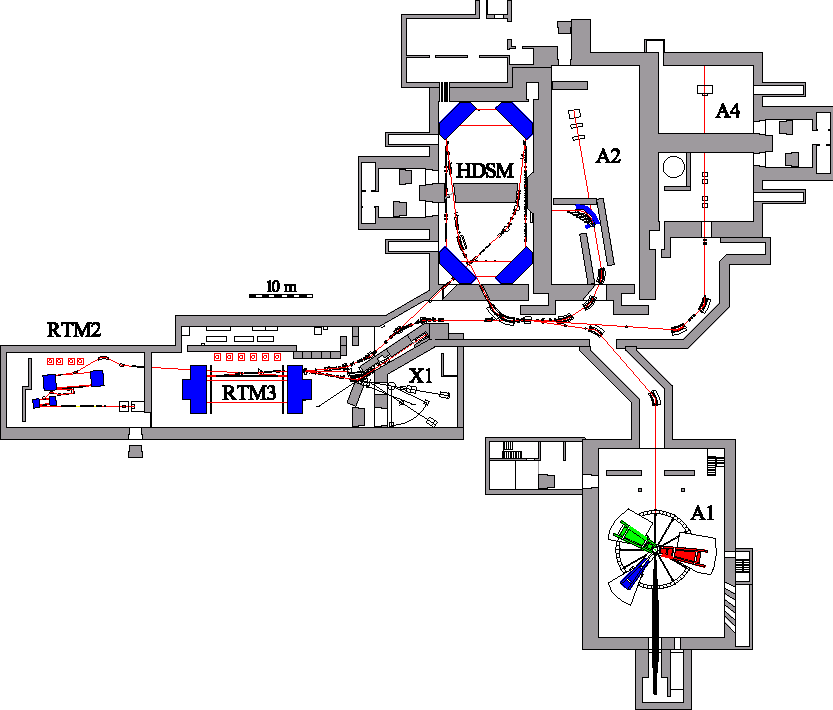
\includegraphics{grundriss}
	\caption[Grundriss der MAMI-Anlage]{Grundriss der Beschleunigeranlage MAMI. Zu sehen sind die drei RTMs, der HDSM der Tagger und die verschiedenen Experimentierhallen: A1 (Elektronenstreuung), A2 (Strukturanalyse von Nukleonen), A4 (Parit\"atsverletzung) und X1 (R\"ontgenstrahlung) \cite{KPh07}.}
	\label{fig.grundriss_anlage}
\end{figure}


\section{Der MAMI-Beschleuniger}
1979 wurde das MAMI erstmals in Betrieb genommen und bestand damals nur aus einem einzelnen RTM, womit eine maximale Elektronenenergie von $14\, \text{MeV}$ erreicht werden konnte. 
Im Laufe der Jahre wurde das MAMI um zwei weitere RTMs und einem HDSM (Harmonic Double Sided Microtron) erweitert, wodurch heutzutage eine Elektronenenergie von ca. $1,6\, \text{GeV}$ erreicht werden kann \cite{KPh11G}. 
\newline


Um unpolarisierte Elektronen zu erzeugen, wird eine Glühkathode auf 1000$^{\circ}$C erhitzt. Dadurch können Elektronen den Heizdraht aufgrund ihrer thermischen Bewegung verlassen. Diese Elektronen werden dann durch ein elektrisches Feld, welches zwischen einer heißen Kathode und einer Anode, erzeugt wird, zur Anode beschleunigt und treten dann durch ein Loch in der Anode aus und werden weiter durch einen Linearbeschleuniger mit einer Frequenz von $2,45\, \text{GHz}$ auf ca. $3,5\, \text{MeV}$ beschleunigt. Diese Frequenz ist für das MAMI typisch und macht es zu einem Dauerstrich-Elektronen-Beschleuniger. Das heißt die Frequenz, mit der die Elektronen-Pakete auftreten, ist größer, als die Frequenz, mit der die Detektoren einzelne Events auflösen können und somit wirkt der Strahl für die Detektoren kontinuierlich.
Am MAMI ist es auch m\"oglich einen spinpolarisierten Elektronenstrahl zu erzeugen, dazu wird ein GaAs Kristall mit polarisiertem Laserlicht bestrahlt. 
In der Strahlzeit, die in dieser Arbeit betrachtet wird, wurde ein unpolarisierter Strahl verwendet.
\newline
Da die Elektronen mit einem Linearbeschleuniger nur einige MeV pro Meter beschleunigt werden k\"onnen, und man keine kilometerlangen Strecke bauen kann, entschied man sich daf\"ur, die Elektronen mehrmals durch den gleichen Beschleunigerabschnitt zu beschleunigen. Dazu werden sie nachdem sie beschleunigt wurden, durch zwei 180$^{\circ}$ Dipole so umgeleitet, dass sie sich wieder am Anfang des Beschleunigerabschnitts befinden und diese Bahn abermals durchlaufen können. Nun besitzen die Elektronen allerdings einen gr\"o{\ss}eren Impuls und werden in einer Bahn mit gr\"o{\ss}erem Radius durch die Dipole geleitet bis die gew\"unschte Energie erreicht wird und der Strahl in den n\"achsten Abschnitt umgeleitet wird. Die Struktur eines RTM erinnert an eine antike Pferderennbahn, daher hat es auch seinen Namen.

 Eine phasengerichtete R\"uckkopplung ist allerdings nur m\"oglich, wenn die statische und die dynamische Koh\"arenzbedingung erf\"ullt sind. Um die statische Koh\"arenzbedingung zu erf\"ullen, muss die L\"ange der ersten vollst\"andigen Bahn ein ganzzahliges Vielfaches der Wellenl\"ange der beschleunigten Hochfrequenz sein. F\"ur die dynamische Koh\"arenzbedingung muss die L\"angendifferenz von zwei aufeinander folgenden Uml\"aufen ebenfalls ein ganzzahliges Vielfaches der Wellenl\"ange sein\cite{Un08}. 
 
 Diese Bedingungen geben ebenfalls die Grenzen f\"ur den maximal m\"oglichen Energiegewinn jeder Stufe an. 
\newline
Wie bereits erw\"ahnt besitzt MAMI drei dieser RTMs. Die erste Stufe MAMI A besteht aus zwei RTMs mit 18 bzw. 51 Uml\"aufen. Die zweite Stufe MAMI B besteht aus dem gr\"o{\ss}ten RTM der Welt mit 90 Uml\"aufen und Dipolen mit einer Breite von jeweils $5\, \text{m}$, wodurch sie $450\, \text{t}$ schwer sind. Damit sind auch die technischen Grenzen erreicht \cite{KPh11F}.


\begin{figure}[h!]
	\begin{center}
	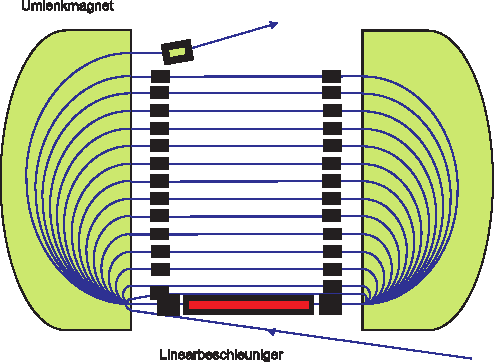
\includegraphics{RTM}	
	\caption[Prinzip eines RTM]{Prinzip eines RTM: Der Elektronenstrahl wird immer wieder durch den Linearbeschleuniger geschickt, bis die gew\"unschte Energie erreicht wird und der Strahl mittels einem sogenannten Kicker-Magnet zum nächsten Abschnitt weiter geleitet wird \cite{KPh07}. }
	\label{fig.RTM}
\end{center}
\end{figure}

Um dennoch höhere Energien zu erreichen, ist ein anderes Konzept erforderlich. MAMI C ist folglich kein reiner RTM mehr, sondern ein HDSM. Das hei{\ss}t, es besteht aus vier 90$^{\circ}$ Dipolen, welche jeweils $250\, \text{t}$ schwer sind und einem zus\"atzlichen Linearbeschleuniger. 
Das bedeutet, dass die Elektronen im HDSM zweimal pro Umlauf beschleunigt werden.

Zwar wird der Rest von MAMI mit einer Hochfrequenz von $2,45\, \text{GHz}$ betrieben, allerdings muss der erste Beschleuniger von MAMI-C aufgrund der Hallenl\"ange mit einer Hochfrequenz von $4,90\, \text{GHz}$ laufen, w\"ahrend der zweite f\"ur eine bessere longitudinale Strahlstabilit\"at mit $2,45 \, \text{GHz}$ betrieben wird \cite{Ca10}.
%F\"ur dieses HDSM wurde der erste Linearbeschleuniger der Welt entwickelt, der mit einer Fequenz von 4,9 GHz laufen kann, betrieben wird er allerdings, wie die beiden voherigen RTMs mit einer Frequenz von 2,45 GHz.
%\newline

\begin{table}[h!]
\centering


		\begin{tabular}{p{3cm}cccc}
		
			& RTM1 & RTM2 & RTM3 & HDSM \\

			\hline
			Eingangsenergie &$3,455\, \text{MeV}$  &  $14,35\, \text{MeV}$& $179,5\, \text{MeV}$  &$854,6\, \text{MeV}$ \\
			Ausgangsenergie &$14,35 \,\text{MeV}$  &  $179,5\, \text{MeV} $&$854,6\,\text{MeV}$  & $1,6\,\text{GeV}$ \\ 
			Anzahl Uml\"aufe&18  &51  &90  &43 \\ 
			Energiegewinn  
			pro Umlauf &$0,559\, \text{MeV}$  & $3,24\, \text{MeV}$ &$7,5 \,\text{MeV}$  & $13,93$ - $16,63 \,\text{MeV}$ \\ 
			
	
		\end{tabular}

		\caption[Technische Daten der Mamibeschleunigerstufen]{Technische Daten der MAMI-Beschleunigerstufen \cite{Un08}.}
		\label{tab.MAMIstufen}

\end{table}

 Am Ende der Beschleunigung besitzt der Elektronenstrahl eine Energie von ca. $1,6 \,\text{GeV}$. Diese kann in Schritten von etwa $15\,\text{MeV}$ eingestellt werden. Sein Durchmesser liegt im Mikrometerbereich, was sehr gute Voraussetzungen f\"ur Pr\"azisionsexperimente sind \cite{KPh07}. 
 
 Das MAMI ist mit \"uber 7000 Stunden im Jahr ca. 81\% des Jahres in Betrieb. Fast 6000 Stunden der Betriebszeit werden f\"ur Experimente genutzt. Wegen technischer Ausf\"alle ist MAMI ca. 200 Stunden pro Jahr au{\ss}er Betrieb. Die restliche Zeit wird zur Vorbereitung und Weiterentwicklung der Beschleunigeranlage genutzt \cite{KPh11B}.
 
 
 \section{Die Photonenmarkierungsanlage}
 
 In der A2-Experimentierhalle wird schlie{\ss}lich der reelle Photonenstrahl mittels Bremsstrahlung erzeugt. Dazu trifft der MAMI-Elektronenstrahl auf einen Radiator, typischerweise eine d\"unne Metallfolie oder ein Diamant mit einer Dicke von 10 bis $100\, \mu\text{m}$. Die Elektronen werden im Coloumbfeld eines Kerns des Radiators beschleunigt und k\"onnen dann, aufgrund der Impulserhaltung ein Photon in Vorw\"artsrichtung ausstrahlen.
 
 \begin{equation}
 e^{-}+N\rightarrow N + e^{-}+\gamma
 \label{eq.Streuung}
 \end{equation}
  Der R\"ucksto{\ss} des Kerns kann aufgrund seiner gro{\ss}en Masse relativ zu der des Elektrons vernachl\"assigt werden und die Energie der Photonen kann anschlie{\ss}end mit folgender Formel berechnet werden:
  
  \begin{equation}
  E_{\gamma}= E_{e^{}}-E'_{e}
  \label{eq.Photonenenergie}
  \end{equation}
 Dabei ist $E_e$ die Energie des einfallenden Elektronenstrahls und $E'_{e}$ die Energie der gestreuten Elektronen, welche durch den Glasgow-Mainz-Tagger (siehe Abbildung \ref{fig.TAGGER}) bestimmt wird.
 % dieser trennt zus\"atzlich den Photonen- von dem Elektronenstrahl. Durch einen Dipol wurden die Elektronen ohne Bremsstrahlung, das hei{\ss}t ohne Energieverlust, abgelenkt und, je nach Energie, auf einen bestimmten Abschnitt des Tagger-Elektronenleiters fokussiert.  
 Dieser ist ein impulsselektierendes, magnetisches Spektrometer, in dem ein homogenes magnetisches Feld angelegt ist, welches die Elektronen auf eine Fokalebene lenkt, hinter der sich die Tagger-Elektronenleiter befindet. Dadurch wird zus\"atzlich der Elektronenstrahl von dem Photonenstrahl getrennt. Dieses Magnetfeld ist außerdem so eingestellt, dass Elektronen, welche keine Energie durch Bremsstrahlung verloren haben, direkt in den Strahlenfang (Beam-Dump) abgelenkt werden. Die restlichen Elektronen werden dann, je nach Impuls, auf einen anderen Abschnitt der Tagger-Leiter fokussiert.
 
 Diese Tagger-Elektronenleiter besteht aus 353 Szintillatoren, welche sich jeweils zur H\"alfte \"uberlappen.
 Dadurch ergeben sich 352 Kan\"ale mit einer Energieaufl\"osung von $\Delta E \approx$  $2\,\text{MeV}$ bzw. $4\,\text{MeV}$ bei einer Strahlenenergie von $E_e=$ $800 \,\text{MeV}$ bzw. $1,6\,\text{GeV}$. 
 
 F\"ur die Daten, welche in dieser Arbeit analysiert werden, wird der EPT (End-Point-Tagger) benutzt. Das Funktionsprinzip des EPT ist \"ahnlich zu dem des Glasgow-Mainz-Taggers, allerdings besitzt der EPT nur 47 Kan\"ale, welche sich im Gegensatz zum Glasgow-Mainz-Tagger nicht \"uberlappen und im oberen Photonenenergieende angebracht sind. Das heißt, bei einer Strahlenergie von $1604\,\text{MeV}$ haben die im End-Point-Tagger registrieren Elektronen durch Bremstrahlung Photonen mit einer Energie von $1420 \,\text{MeV}$ bis $1580\,\text{MeV}$ ausgesandt. Um den End-Point-Tagger zu verwenden, muss die Strahlf\"uhrung leicht ge\"andert werden.
 
 %Folglich lässt sich der Impuls, durch Kenntnis des Auftrefforts des Elektron auf der Tagger-Leiter bzw. im EPT und der St\"arke des Magnetfeldes, bestimmen und dadurch auch die Energie der Elektronen. 

Der Impuls der gestreuten Elektronen l\"asst sich folglich durch die Auftreffposition der Elektronen auf der Tagger-Leiter bzw. im EPT und der St\"arke des Magnetfeldes bestimmen. 
 
 Nun ist die Energie des Elektronenstrahls und die der gestreuten Elektronen bekannt und damit kann schlie{\ss}lich die Energie der Photonen mit Gleichung \ref{eq.Photonenenergie} berechnet werden.
\newline 
\begin{figure}[h!]
	\begin{center}
	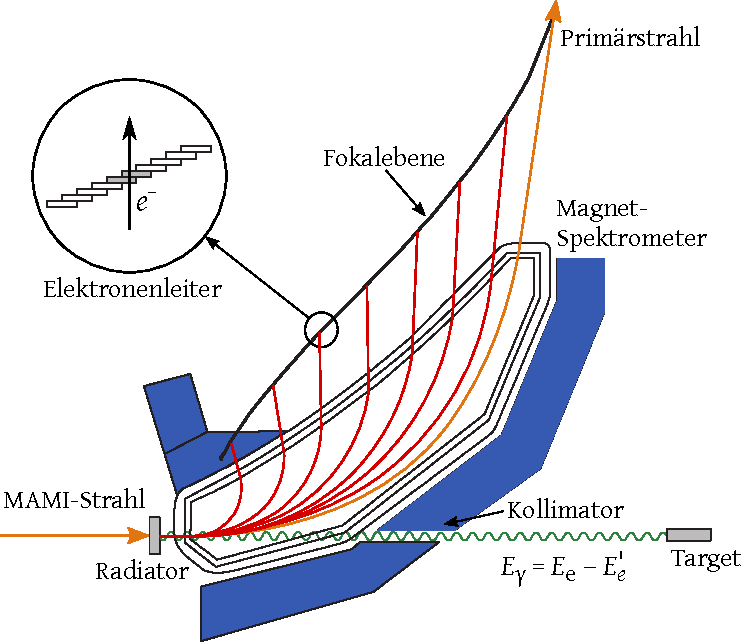
\includegraphics{TAGGER-New}
	
	\caption[Prinzip des Glasgow-Mainz-Taggers]{Der Glasgow-Mainz-Tagger: Am Radiator entstehen durch Bremsstrahlung Photonen, welche den Kollimator passieren und auf das Target treffen. Die Elektronen werden durch den Dipol auf die Elektronenleiter abgelenkt, wodurch sich ihre Energie bestimmen lässt \cite{Un08}.}
\label{fig.TAGGER}	
\end{center}
\end{figure}
 
\section{Das Detektorsystem}
\label{sec:Das-Detektorsystem}
Nach seiner Erzeugung trifft der Photonenstrahl auf ein ca. $10\,\text{cm}$ langes Flüssig-Wasserstoff-Target, welches sich im Zentrum des Crystal-Balls (CB) befindet. Die Reaktionsprodukte können dann durch ein System von Detektoren, bestehend aus dem Crystal-Ball Detektor, einem Teilchenidentifikationsdetektor (PID: Particle Identification Detector), zwei Vieldrahtproportionalkammern (MWPC: Multi-Wire Proportional Chamber) und einem Photonenspektrometer (TAPS: Two Arm Photon Spectrometer) nachgewiesen werden. Der PID und die MWPC sind im Inneren des CB angebracht. Das TAPS wurde am Ausgang des CB platziert, um einen fast vollständig abgedeckten Raumwinkel zu erreichen.
\begin{figure}[h!]
	\begin{center}
		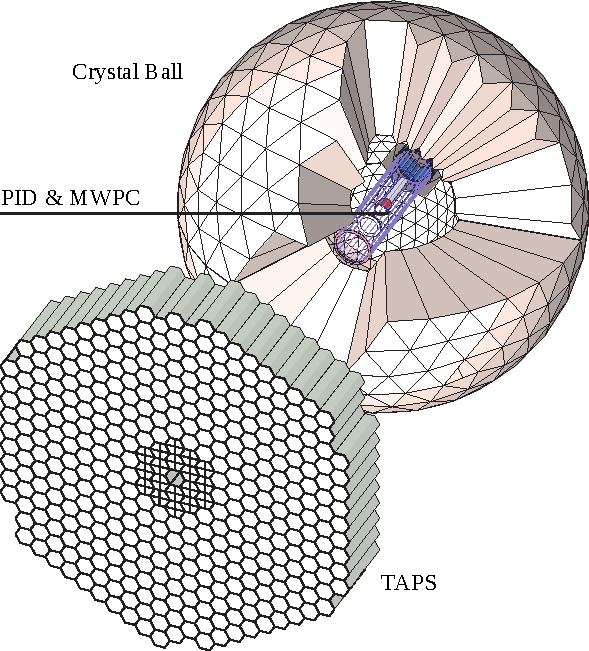
\includegraphics{crystal_ball}
	
		\caption[Anordnung des Detektorsystems] {Anordnung des Detektorsystems: Im Zentrum des sph\"arischen Kalorimeters (CB) befinden sich der Detektor zur Teilchenidentifikation (PID) und zwei zur Bestimmung der Teilchen-Trajektorie (MWPC). Die TAPS-Wand befindet sich am Ausgang des CB und sorgt daf\"ur, dass der CB einen Raumwinkel von fast 4$\pi$ abdeckt \cite{We13}.}
		\label{[fig.crystal_ball]}	
\end{center}
\end{figure}

\subsection{Der Crystal-Ball-Detektor}
Ursprünglich wurde der Crystal-Ball Detektor Anfang der 70er Jahre am SLAC (Stanford Linear Accelerator Center) entwickelt und zur Untersuchung des $J/\Psi$-Mesons am SPEAR (Stanford Positron Electron Asymmetric Ring) eingesetzt. Später wurde mit seiner Hilfe das Bottom-Quark am DESY (Deutsches Elektronen-Synchrotron) und die Baryonenresonanzen am BNL (Brookhaven National Laboratory) untersucht.
Seit November 2002 steht der Crystal-Ball Detektor der A2-Kollaboration am MAMI für Experimente mit reellen Photonen zur Verfügung.
\newline
Der Crystal-Ball ist ein Kalorimeter, bestehend aus 672 Natriumiodid (NaI) Szintillatoren, welche so angeordnet sind, dass ca. 94\% des Raumwinkels abgedeckt werden. Die Geometrie basiert auf der Form eines Ikosaeders, ein Polyeder bestehend aus 20 gleichgro{\ss}en gleichseitigen Dreiecken. Jedes dieser Dreiecke ist weiter aufgeteilt in vier kleinere gleichseitige Dreiecke, welche wiederum jeweils in neun gleichseitige Dreiecke unterteilt sind. Somit ergeben sich 720 gleichseitige Fl\"achen. Aufgrund der hohen Anzahl der Fl\"achen erinnert der Crystal-Ball an eine Hohlkugel mit einem Au{\ss}enradius von ca. $66\,\text{cm}$ und einen Innenradius von ca. $25\,\text{cm}$. 

Da der Crystal-Ball Detektor urspr\"unglich in $e^+e^-$ Streuexperimenten verwendet wurde, mussten sowohl f\"ur den Strahlenein-, als auch -ausgang 24 dieser Fl\"achen entfernt werden, wodurch insgesamt 672 Detektoren angebracht werden k\"onnen. Diese Detektoren bestehen aus NaI-Szintillatorkristallen und sind ca. $40\,\text{cm}$ ($\sim$15,7 Strahlungsl\"angen) lang und haben die Form eines Pyramidenstumpfes mit dreieckiger Grundfl\"ache und einer Seitenl\"ange von etwa $5\,\text{cm}$ am schmalen und ca. $13\,\text{cm}$ am dicken Ende. Jeder dieser Kristalle ist optisch durch reflektierendes Papier und aluminisierten Mylar durch seine umliegenden Nachbarn isoliert. Ein einzelner Kristall deckt etwa 0,14 \% des Raumwinkels ab und wird durch einen eigenen Photoelektronenvervielfacher (PMT: PhotoMultiplier-Tube) ausgelesen. 



\subsection{TAPS, PID \& MWPC}
\label{sec:TAPS-PID-MWPC}
Der PID besitzt eine zylindrische Form mit einem Durchmesser von $116,5\,\text{mm}$ und besteht aus 24 einzelnen Szintillatoren, welche jeweils $500 \,\text{mm}$ lang, $15,3\,\text{mm}$ breit und $4 \,\text{mm}$ dick sind. Da die Szintillatoren nur eine geringe Dicke im Verhältnis zu ihrer Strahlungslänge aufweisen, verlieren Photonen beim durchfliegen weniger als 1\% ihrer Energie. Geladene Teilchen auf der anderen Seite erfahren einen Energieverlust $\Delta E$. Ihre restliche Energie wird dann an den Crystal-Ball abgegeben. Folglich kann man durch den PID zwischen geladenen und ungeladenen Teilchen unterscheiden. 

Au{\ss}erhalb des PIDs sind die MWPCs angebracht. Dabei handelt es sich um zwei, aus Anodendr\"ahten aufgebauten, Protortionalz\"ahler in Form von Hohlzylindern. Die Anodendr\"ahte sind parallel zur Strahlenachse ausgerichtet und befinden sich zwischen zwei Lagen von spiralf\"ormigen Kathodenstreifen. 

Da der Crystal-Ball zwei \"Offnungen f\"ur den Strahlenein- und -ausgang besitzt, wird f\"ur die Fixed-Target Experimente die TAPS-Wand verwendet.
%Da die A2-Kollaboraions Experimente mit einem Fixed-Target untersucht und der Crystal-Ball zwei \textit{L\"ocher} f\"ur einen Strahleneingang und -ausgang besitzt, wurde die TAPS-Wand entwickelt. 
Diese deckt einen Polarwinkel zur Strahlenachse von 1,2$^{\circ}$ bis 20$^{\circ}$ ab. Sie wurde etwa $1,5\,\text{m}$ vom Mittelpunkt des CB entfernt positioniert und besteht aus 72 PbWO$_4$ und 366 BaF$_2$ Szintillatorkristallen. 
 Somit wird mit diesem Detektorsystem ein Raumwinkel von fast 97\% abgedeckt.

\section{Szintillatoren}
\label{sec:Szintillatoren}
Dringen hochenergetische Photonen und Elektronen in Materie ein, so entstehen elektromagnetische Schauer
%In Materie entstehen elektromagnetische Schauer durch hochenergetische Elektronen und Photonen 
\cite{Leo87}.
Gelangt ein hochenergetisches Photon in Materie so entsteht durch Paarbildung ein Positron-Elektron-Paar. Dafür muss das Photon eine Energie von mindestens $2\cdot m_{e^-} = 1,022\,\text{MeV}$ besitzen. Diese Energie verteilt sich dann gleichmäßig auf das Elektron und das Positron. Da diese beiden Teilchen geladen sind und sich ihre Geschwindigkeit im elektromagnetischen Feld eines Atomkerns ändert, erzeugen sie durch Bremsstrahlung wieder Photonen. Diese Prozesse wiederholen sich, sodass ein Schauer entsteht, welcher sich kaskadenartig ausbreitet. Die Energien der Teilchen nehmen dabei immer weiter ab, bis die kritische Energie $E_c$ erreicht wird. Bei dieser Energie entspricht der Energieverlust durch Bremsstrahlung dem Energieverlust, der durch Ionisation entsteht.

Fällt die durchschnittliche Energie eines Elektron auf $E_0/e$, so wird die dafür benötigte Strecke $X_0$ Strahlungslänge genannt.
\newline

Nimmt man an, dass die Elektronen und die Photonen nach etwa einer Strahlungslänge wechselwirken, und dass die Teilchen jeweils die Hälfte ihrer Energie abgeben, so lässt sich die Gesamtzahl der Teilchen und die Energie eines einzelnen Teilchen nach $t$ Kaskaden berechnen durch\cite{Leo87}:

\begin{equation}
N\approxeq 2^t
\end{equation}
\begin{equation}
E(t) \approxeq \frac{E_0}{2^t}
\end{equation}

Dieser Schauer breitet sich, sowohl in longitudinaler als auch transversaler Richtung aus. Diese transversale Ausbreitung kann durch den Moli\'ere-Radius beschrieben werden. 
Dieser wird berechnet durch \cite{Leo87}:

\begin{equation}
R_M = 21\, \textnormal{MeV}\cdot \frac{X_0}{E_c}
\end{equation}

95\% aller im Schauer entstanden Teilchen, befinden sich innerhalb von zwei Moli\'ere-Radien. 

















\chapter{Werkzeuge}
\label{chap:Wergzeuge}
\section{Verwendete Programme}

Die physikalische Analyse wird mit Ant (Analysis Toolkit) durchgef\"uhrt. Mit Ant ist es m\"oglich, verschiedene Informationen aus dem Detektorsystem zu erhalten und damit können verschiedene Bedingungen zur Auswertung der Daten festzulegen werden. Ant benutzt dazu ROOT. Mit Ant ist es m\"oglich sowohl Daten aus einer Strahlzeit, als auch Daten, welche in einer Simulation erzeugt wurden, zu analysieren \cite{Ant17}.

ROOT ist ein wissenschaftliches Software Framework, welches zur Verwaltung, Analyse, Visualisierung und Lagerung von gro{\ss}en Datens\"atzen eingesetzt wird \cite{Ce97}.

Als Ereignisgenerator wird zun\"achst auf Pluto zur\"uckgegriffen. Pluto ist ein auf Monte-Carlo Methoden basierendes Simulation Framework f\"ur Reaktionen mit schweren Ionen und f\"ur Hadronen-Physik. Der Vorteil von Pluto ist, dass Reaktionen bereits mit wenigen Befehlen in ROOT aufgesetzt werden k\"onnen \cite{Pl07}. 

Mit einem Ereignisgenerator ist es allerdings nur m\"oglich den Zerfall und die Reaktionsprodukte zu erzeugen. Das Verhalten des Detektorsystems wird dadurch nicht simuliert. Dazu wird auf Geant4 zur\"uckgegriffen. Geant4 ist ein Toolkit f\"ur Simulationen, welches das Durchdringen von Teilchen durch Materie mit Hilfe von Monte-Carlo-Methoden beschreibt \cite{Ge04}.

Alle diese Programme basieren auf der Programmiersprache C++.

\section{Algorithmus zur Clusterbildung}
\label{sec:Clustering-Algorithmus}

Wie bereits in Abschnitt \ref{sec:Szintillatoren} erw\"ahnt wurde, wird ein elektromagnetischer Schauer aus Elektronen, Positronen und Photonen erzeugt, wenn ein hochenergetisches Photon einen Detektorkristall trifft. Dieser Schauer breitete sich aus und dringt in benachbarte Kristalle ein. Folglich wird nicht die gesamte Energie eines Photons an einen Kristall abgegeben, sondern immer auch an seine Nachbarn. Würde man größere Kristalle verwenden, um diesen Effekt zu vermeiden, dann könnte man die Position des Auftreffortes nicht mehr so genau bestimmen.

Damit ein Kristall als ausgel\"ost eingestuft wird, m\"ussen zwei Bedingungen erf\"ullt werden.
Das Analogsignal des Photomultipliers muss die eingestellte Diskriminatorschwelle von jeweils $1,1 \,\text{MeV}$ und eine Energieschwelle, welche in der Analyse gesetzt wird, \"uberschreiten.
Sind diese beiden Bedingungen erf\"ullt, wird der Kristall in der weiteren Analyse mit einbezogen.
 
 Der Cluster Algorithmus wird angewandt, um sowohl die Energie des detektierten Photons, als auch seinen genauen Auftreffort im Crystal-Ball zu bestimmen.
 Dieser Algorithmus ist in drei Phasen aufgeteilt.
 
 In der ersten Phase werden alle Kristalle die ausgel\"ost wurden und sich an mindestens einer Ecke ber\"uhren zu einem Cluster zusammengefasst. Folglich kann es auch mehrere Cluster geben.
 
 In der zweiten Phase werden lokale Maxima in jedem Cluster gesucht. Dazu wird in jedem Kristall ein Vote gesetzt. Besitzt einer seiner Nachbarn mehr Energie, so wird sein Vote zu diesem Kristall verschoben. Besitzt ein einzelner Kristall alle Votes, so bleibt der Cluster unver\"andert. Andernfalls wird an jedem dieser Maxima nummeriert mit $k$ ein sogenannter Bump mit der Position $\vec{b}_k$ definiert. Von diesem kann die Energie mit einer Gewichtung berechnet werden, die von der Energie der einzelnen Kristalle und dem Moli\'ere Radius abh\"angt. Mit dieser Gewichtung und einer zus\"atzlichen Gewichtung, welche logarithmisch von der gewichteten Energie der Kristalle und der Gesamtenergie des Bumps anh\"angt, kann die Position des Bumps neu berechnet werden. Von diesem wird erneut die Energie berechnet und die Schritte wiederholen sich, bis die Bump Position stabil ist, dabei kann es auch passieren, dass sich zwei Bumps vereinen, wenn sie zu dicht aneinander liegen, oder eine Maximale Anzahl an Iterationen erreicht wird.
 
 In der letzten Phase werden die Bumps benutzt, um die Cluster aufzuteilen. Dazu l\"ost jeder Bump einen Grass-Fire Algorithmus aus, um partielle Cluster mit einer Energie $E^k_{\text{split}}$ zu bilden. Gestartet wird hier beim Kristall mit dem gr\"o{\ss}ten Gewicht innerhalb eines Bumps. Mit jeder Grass-Fire Iteration wird die Energie seiner Nachbarn zu $E^k_\text{{split}}$ aufaddiert. Sobald ein Kristall durch zwei oder mehr Bumps in der Grass-Fire Iterationsschritt angesprochen wird, wird seine Energie auf die jeweiligen partiellen Cluster verteilt. 
 F\"ur mehr Details siehe \cite{Ne17}.
 

\begin{comment}

Wie bereits in Abschnitt \ref{sec:Szintillatoren} erw\"ahnt wurde, breitet sich ein elektromagnetischer Schauer aus Elektronen, Positronen und Photonen aus, wenn ein Photonen einen Detektorkristall trifft. Dieser Schauer breitet sich aus und dringt in benachbarte Kristalle ein. Folglich wird nicht die gesamte Energie eines Photons an einen Kristall abgegeben, sondern immer auch an seine Nachbarn. 

Damit ein Kristall als ausgel\"ost eingestuft wird, m\"ussen zwei Bedingungen erf\"ullt werden.

Das Analogsignal des Photomultipliers muss die eingestelle Diskriminatorschwelle von jeweils 1,1 MeV und eine Energieschwelle, welche in der Analyse gesetzt wird, \"uberschreiten.

Sind diese beiden Bedingungen erf\"ullt, wird der Kristall in der weiteren Analyse mit einbezogen.

\begin{figure}[h!]
	\begin{center}
		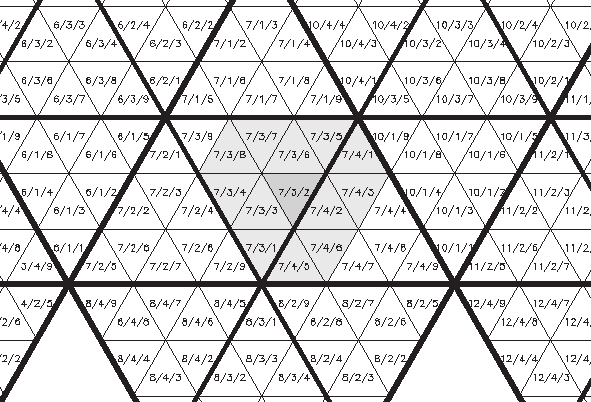
\includegraphics[width=100mm]{ClusterBeispiel}
		\caption[Clusterbildung]{Kristall 7/3/2 (dunkelgrau) stellt beispielhaft einen Zentralkristall dar. Seine n\"achsten Nachbarn sind hellgrau unterlegt. Sie liegen ringf\"ormig um den zentralen Kristall \cite{Un08}.}
		\label{fig:Cluster-Bildung}	
	\end{center}
\end{figure}

Zun\"achst wird der Kristall gesucht, der den h\"ochsten Energiebetrag hat. Dieser wird als Zentralkristall im Cluster gesetzt. In Abbildung \ref{fig:Cluster-Bildung} ist dieser dunkelgrau unterlegt. Zu dieser Energie wird die Energie seiner n\"achsten (maximal 12) Nachbarn aufaddiert. Diese n\"achsten Nachbarn sind hellgrau unterlegt. Als n\"achster Kristall ist ein Kristall definiert, wenn er den zentralen Kristall mit mindestens einer Ecke ber\"uhrt. Folglich besitzen Detektoren am Rand des Strahlenein- bzw. -ausgangs weniger n\"achste Nachbarn. 

Innerhalb dieser 13 Kristalle wird 98\% der Energie deponiert \cite{Un08}. Um den genauen Auftreffort $\vec{r}_{Cl}$ zu bestimmen, benutzt man nicht nur die Lage des zentralen Kristalls. Stattdessen werden alle im Cluster miteinbezogene Kristalle ber\"ucksichtigt.

\begin{equation}
\vec{r}_{Cl}=\frac{\sum_{i}^{}\vec{r}_i\sqrt{E_i}}{\sum_{i}^{}\sqrt{E_i}}
\end{equation}

Dabei ist $\vec{r}_i$ eines Kristalls im Cluster und $E_i$ die von diesem Kristall gemessene Energie. Au{\ss}erdem wird mit der Wurzel der Energie der einzelnen Kristalle gewichtet.

\end{comment}















\chapter{Vorbereitungen}
\label{chap:Vorbereitung}


\section{Umstellung auf die Crystal-Ball-Fitfunktion}
\label{sec:CB-Funktion}

Um die Masse des $\pi^0$ zu bestimmen, werden Histogramme mit der errechneten invarianten Masse erzeugt. Ein $\pi^0$ zerf\"allt gr\"o{\ss}tenteils in zwei Photonen. Bereits bei diesen Histogrammen werden nur Photonenpaare ber\"ucksichtigt, wenn sich die Energien bei beiden Photonen um maximal $25 \,\text{MeV}$ unterscheiden. Durch diese Bedingung k\"onnen Aussagen \"uber das Verhalten des Crystal-Balls bei verschiedenen Energien getroffen werden.
 Anschlie{\ss}end wird \"uber diese Histogramme mit einer Funktion gefittet, um die Position des Peaks zu bestimmen.

Zum Fitten wurde zun\"anchst auf ein bereits existierendes Fitmodul zur\"uckgegriffen. Dieses ist eine Summe aus einer Gau{\ss}funktion und einem Polynom vierten Grades. Allerdings entspricht die Form des $\pi^0$-Peaks nicht der einer Gau{\ss}verteilung, weswegen nach einer alternativen Fitfunktion gesucht werden muss. 

Bei dieser neuen Funktion handelt es sich um die Crystal-Ball Funktion, welche nach der Crystal-Ball Kollaboration benannt ist. Diese Funktion ist eine Dichtefunktion einer asymmetrischen Wahrscheinlichkeitsverteilung und ist in zwei Bereiche aufgeteilt. Im zentralen Bereich entspricht sie einer Gau{\ss}form, diese geht f\"ur kleine Werte in eine Potenzreihe \"uber.

\begin{equation}
f(x|\alpha,n,\bar{x},\sigma)=N\begin{cases}e^{-\frac{(x-\bar{x})^2}{2\sigma^2}}, \,\textnormal{falls $\frac{x-\bar{x}}{\sigma}> -\alpha$} \\
A(B-\frac{x-\bar{x}}{\sigma})^{-n},\, \textnormal{falls $\frac{x-\bar{x}}{\sigma}\leqslant -\alpha$} 
\end{cases}
\label{eq:Crystal-Ball-Funktion}
\end{equation}

Dabei ist $N$ der Normierungsfaktor, $\bar{x}$ der Erwartungswert und $\sigma$ die Standardabweichung der Gau{\ss}funktion. Der Parameter $\alpha$ gibt die Position an, an dem die Gau{\ss}verteilung in das Potenzgesetz mit dem freien Parameter $n$, \"ubergeht\cite{Ce15}.



Diese ist bereits gr\"{\ss}tenteils in Ant implementiert, lediglich die Normierung muss noch nachtr\"aglich hinzugef\"ugt werden.
Der Untergrund wird weiterhin mit einem Polynom vierten Grades angen\"ahert.

\begin{figure}[h!]
	\begin{center}
		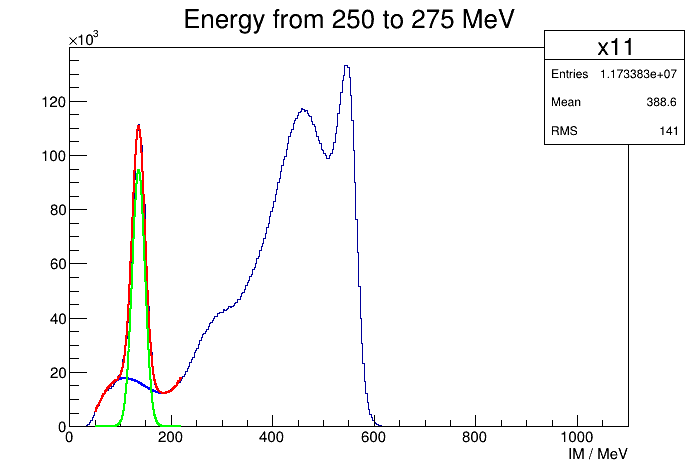
\includegraphics[width=100mm]{NewCalib/Strahlzeit2014/20171904RealIntervalFitExample}
		
		\caption[Strahlzeit: Beispielfit f\"ur die Crystal-Ball-Fitfunktion]{Beispiel eines Fits. Es handelt sich dabei um das Photonenenergieintervall von $250 \,\text{MeV}$ bis $275\,\text{MeV}$.
			Zu erkennen ist der Untergrundfit (Blau), der Crystal-Ball-Fit (Gr\"un) und die Addition der beiden Fits (Rot). %Alle weiteren Fits mit dieser Bedingung sind in Abbildung \ref{fig:similarenergyallfits} zu sehen.
		}
		\label{fig:fitexampleenergyinterval0903}	
	\end{center}
\end{figure}

In Abbildung \ref{fig:fitexampleenergyinterval0903} ist ein Beispiel f\"ur einen Fit mit der Crystal-Ball Funktion abgebildet. Das Polynom ist hier Blau dargestellt. Die Crystal-Ball Funktion ist hier in Gr\"un zu sehen. Damit leichter \"uberpr\"uft werden kann, ob der Fit sinnvoll ist, werden beide Fits addiert und zus\"atzlich in den Graphen gezeichnet (Rot). Der in der Crystal-Ball Funktion bestimmte Wert von $\bar{x}$ gibt dann die errechnete invariante Masse des $\pi^0$ an.


\section{Reduzierung des Untergrunds}

Im Crystal-Ball Detektor werden nicht nur Photonen, sondern alle m\"oglichen Teilchen detektiert. Folglich werden auch viele Teilchen registriert, die man nicht betrachten will. Diese erzeugen zus\"atzlich einen Untergrund, der die Genauigkeit des Fits verschlechtert.

Zu erahnen ist dies bereits in Abbildung \ref{fig:fitexampleenergyinterval0903}. Hier ist der $\pi^0$-Peak bei einer invarianten Masse von $135\,\text{MeV}$ und der $\eta$-Peak bei ca. $550\,\text{MeV}$ zu sehen. Beide Peaks werden allerdings durch den Untergrund gest\"ort. %Der Fokus dieser Arbeit lag zwar bei der Betrachtung des $\pi^0$, allerdings war es auch interessant die Position des $\eta$-Peaks zu betrachten,
 Daher wird nach einem Weg gesucht, den Untergrund m\"oglichst stark zu reduzieren. 

Deswegen wird nun auch \"uberpr\"uft, ob die detektierten Teilchen eine Ladung besitzen. M\"oglich ist dies durch den PID-Detektor. Sind die detektierten Teilchen geladen, dann handelt es sich nicht um Photonen und sie werden verworfen. Dies f\"uhrt zu einer Reduzierung des Untergrunds. Zu sehen ist das in Abbildung \ref{fig:Reduzierter-Untergrund-Fit}.


\begin{figure}[h!]
	\begin{center}
		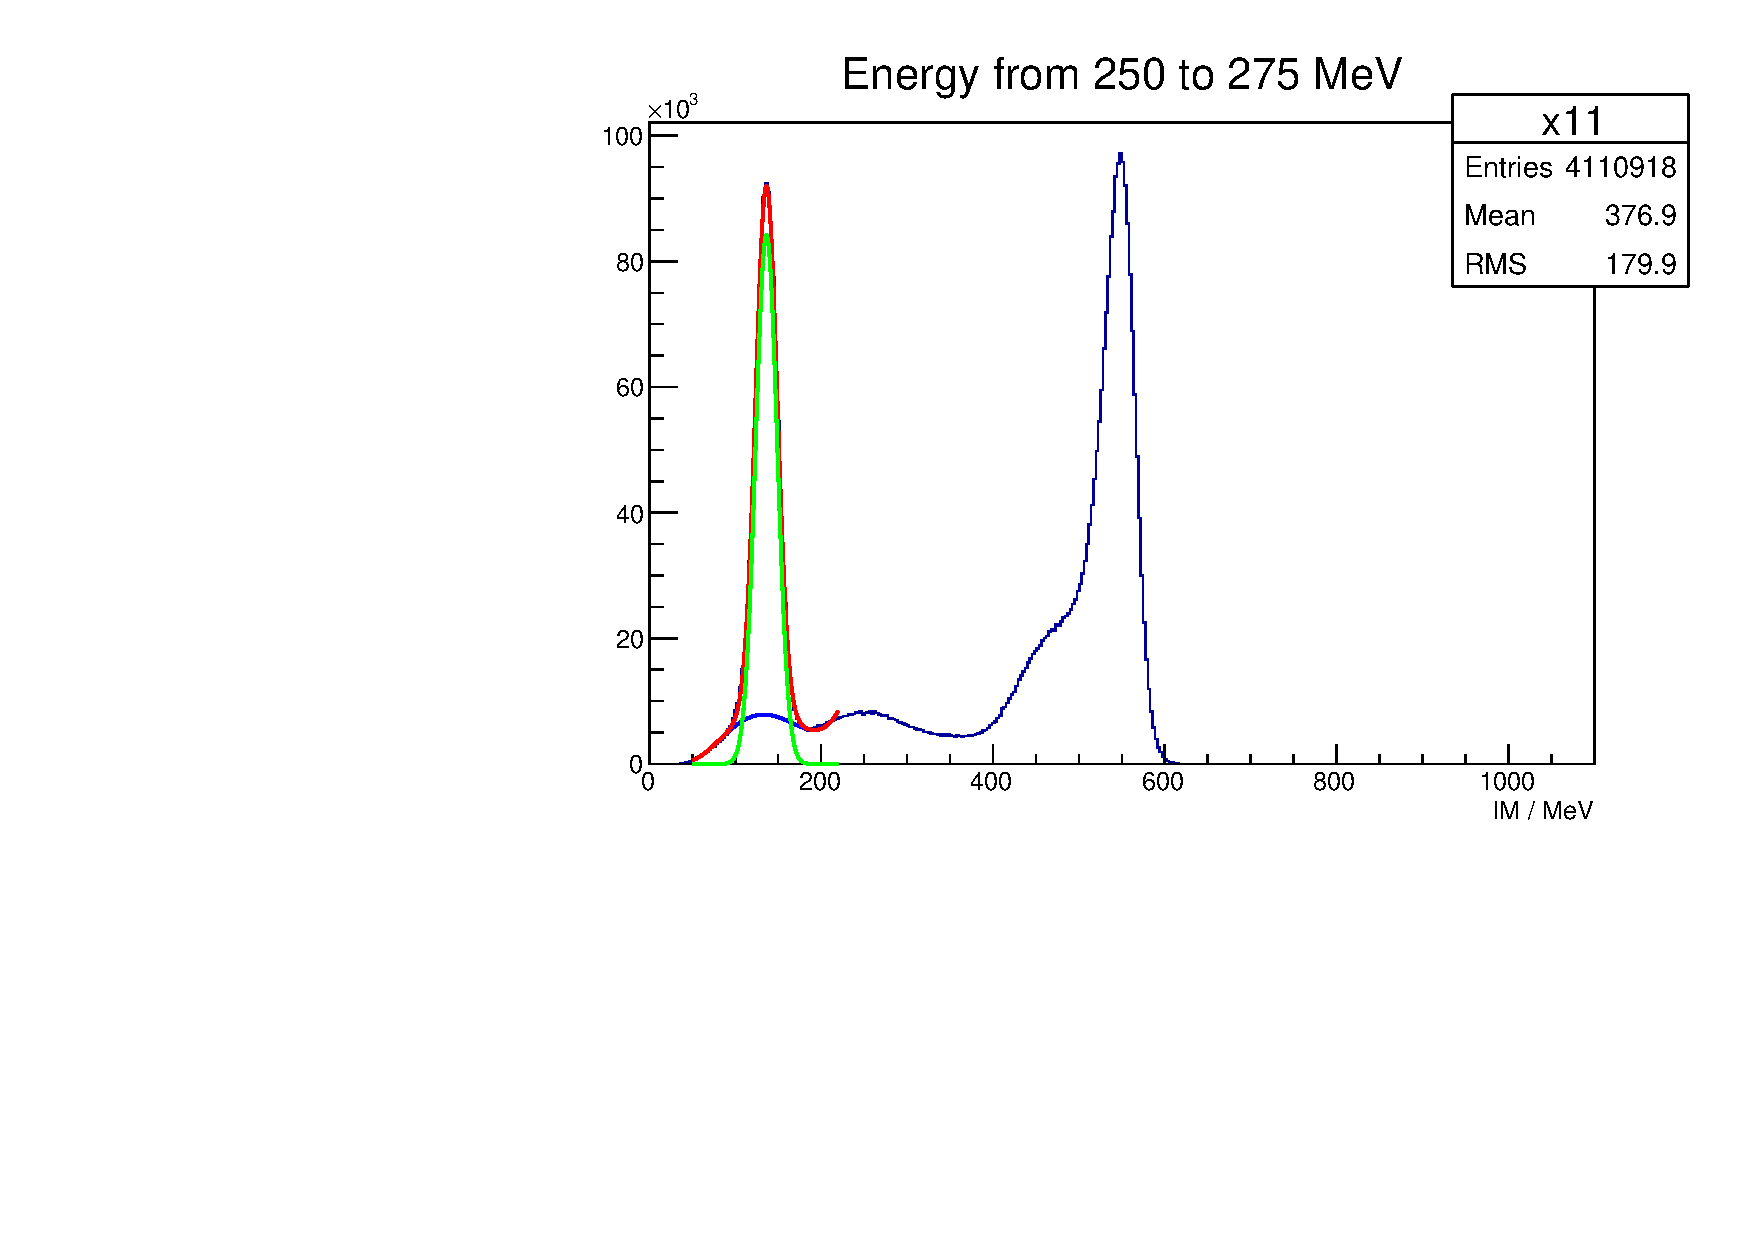
\includegraphics[width=100mm]{NewCalib/Strahlzeit2014/20171904RealUnchargedFitExample}
	\end{center}
\caption[Strahlzeit: Beispiel eines Fits mit reduziertem Untergrund]{Beispiel eines Fits mit reduziertem Untergrund. Es handelt sich dabei um das Photonenenergieintervall von $250\,\text{MeV}$ bis $275\,\text{MeV}$. Sowohl der $\pi^0$-Peak bei $135 \,\text{MeV}$, auch als der $\eta$-Peak bei $550\,\text{MeV}$ sind deutlich zu erkennen. Alle Fits zur dieser Bedingung sind in \ref{fig:similarenergyallfitsuncharged} zu sehen.}
\label{fig:Reduzierter-Untergrund-Fit}
\end{figure}

 Hier erkennt man direkt, dass sich der Untergrund vermindert hat, sodass die beiden Peaks deutlich zu erkennen sind. Daraus folgt, dass auch besser \"uber diese Peaks gefittet werden kann, was zur Folge hat, dass die Position des Peaks der invarianten Masse besser bestimmt werden kann.


\section{Umstellung auf einen neuen Ereignisgenerator}
\label{sec:Vorbereitung-der-Simulation}

Da viele Informationen \"uber die Prozesse im Experiment nicht durch die Detektoren bestimmt werden k\"onnen, ist es hilfreich, auf Simulationen zur\"uckzugreifen. Daf\"ur stehen verschiedene Softwarepakete zur Verf\"ugung, in denen unterschiedliche Prozesse simuliert wurden.

So gibt es bereits vorgefertigte Pakete, wie den Cocktail.
Im diesem sind ca. 250 Millionen Prozesse aus Photoproduktion für EPT Photonenenergien zwischen $1420\,\text{MeV}$ bis $1580\,\text{MeV}$ enthalten. Allerdings sind im Cocktail nicht nur $\pi^0 \rightarrow \gamma \gamma$ Prozesse enthalten, sondern auch viele andere.

Die Zerf\"alle im Cocktail sind bereits komplett durchsimuliert. Das hei{\ss}t, sowohl der Zerfall der Teilchen, als auch das Verhalten der Detektoren wurde simuliert, wodurch der Cocktail wie eine reale Strahlzeit mit prompt-random Subtraktion behandelt werden kann. Das hei{\ss}t, es werden nur Prozesse betrachtet, die ein Photon mit einer Energie von $1420\,\text{MeV}$ bis $1580\,\text{MeV}$ als Eingangsteilchen besitzen. Diese Bedingung wird gesetzt, um die Simulaiton so klein wie m\"oglich zu halten, da man sonst auch sehr viele Prozesse mit kleinen Photonenstrahlenergien simulieren muss.

Da in dieser Arbeit das Hauptaugenmerk auf Photonen liegt, welche durch den Prozess $\pi^0 \rightarrow \gamma \gamma$ entstehen und eine \"ahnliche Energie besitzen, stellte sich relativ schnell heraus, dass der Cocktail nicht genug relevante Prozesse enth\"alt, nachdem alle unerw\"unschten heraus gefiltert wurden. 

Deshalb wurde zun\"achst ein neues Paket mit mehr Prozessen erstellt. 
Dieses Paket beinhaltet $10^7$ $\pi^0 \rightarrow \gamma \gamma$ Prozesse, welche durch Pluto mit einer Photonenstrahlenergie zwischen $1420\,\text{MeV}$ und $1580\,\text{MeV}$ generiert wurden. Das Verhalten des Crystal-Ball Detektors wurde anschlie{\ss}end mit Geant4 simuliert.

Das Erstellen dieses neuen Paketes nahm sehr viel Zeit in Anspruch, da das Simulieren der Detektoren sehr aufw\"andig ist. So dauert das Erstellen eines Paketes mit $10^5$ Prozessen etwa zwei Stunden. 

Da nur Photonen mit einer \"ahnlichen Energie betrachtet werden, m\"ussen auch von diesem Paket die meisten Zerf\"alle verworfen werden. So kommt es, dass selbst das Paket mit $10^7$ Prozessen nicht genug Photonenpaare mit \"ahnlicher Energie enth\"alt, da vor allem in den Kapitel \ref{sec:Z-Vertex-Abhaengigkeit} und \ref{sec:Unterschied-Oeffnungswinkel-ZVertex} sehr viele Prozesse ben\"otigt werden.

Um nun aber eine noch größere Simulation zu vermeiden, wurde ein neuer Ereignisgenerator geschrieben, bei dem die gew\"unschten Bedingungen bereits im Eventgenerator eingebaut werden k\"onnen, sodass die Teilchen, welche sowieso verworfen w\"aren, gar nicht erst durch Geant simuliert wurden. 
Damit der neue Ereignisgenerator auch alle relevanten Informationen beinhaltet, muss folgender Prozess betrachtet werden:
%Da man aber trotzdem keine Informationen \"uber die Prozesse verlieren wollte, mussten alle Schritte des folgendes Zerfalls einzeln untersucht und anschließend in die Gun eingebaut werden. 

\begin{equation}
\gamma + p \rightarrow p + \pi^0 \rightarrow p + \gamma \gamma 
\end{equation}

Da die einfallenden Photonen durch Bremsstrahlung erzeugt werden, sind ihre Energien nicht eindeutig, sondern liegen in einem gewissen Intervall. Also muss als erstes die Energie der eingehenden Photonen gew\"urfelt werden.

Dann begibt man sich ins Schwerpunktsystem des einfallenden Photons und des ruhenden Protons $p$. 
Von diesem System kann dann die Schwerpunktsenergie $\sqrt{s}$ ausgerechnet werden:

\begin{equation}
\sqrt{s}= \sqrt{2E_{\gamma}m_p+2m_p^2}
\end{equation}

Anschlie{\ss}end wird angenommen, dass die Reaktion des Protons mit dem Photon ein $\pi^0$ aussendet. Die Richtung in der dieses $\pi^0$ ausgesandt wird, wird auch wieder mit einem Zufallsgenerator bestimmt. Die Richtung ist also im Raum gleich verteilt.

Da wir uns im Schwerpunktssystem des Protons und des $\pi^0$ befinden, muss aufgrund der Impulserhaltung gelten, dass der Impuls des Protons in die entgegengesetzte Richtung zum $\pi^0$ zeigt, und dass der Betrag der beiden Impulse gleich sein muss. Auch muss aufgrund der Energieerhaltung gelten, dass die Energie der beiden Teilchen addiert gleich der Schwerpunktsenergie ist. Es liegen also die folgenden Formeln vor:


\begin{equation}
|\vec{p}_{\pi^0}|=|\vec{p}_p| = |\vec{p}| 
\end{equation}

\begin{equation}
 \sqrt{s}=\sqrt{m_{\pi^0}^2+\vec{p}^{\,2}} + \sqrt{m_{p}^2+\vec{p}^{\,2}}
\label{eq:Impuls}
\end{equation}


Gleichung \ref{eq:Impuls} kann nach dem Impuls $|\vec{p}|$ aufgel\"ost werden, da die Masse der beiden Teilchen und die Schwerpunktsenergie bekannt ist. Damit kann ihr Impuls und damit auch ihre Energie über $E=\sqrt{m^2+\vec{p}^{\,2}}$ ausgerechnet werden. 
Nun verl\"asst man das Schwerpunktssystem. Dazu werden beide Teilchen wieder in das Laborsystem geboostet.

Weiter muss angenommen werden, dass das $\pi^0$ instantan in zwei Photonen zerf\"allt. Diese Annahme ist nicht abwegig, da die Lebenszeit eines $\pi^0$ nur ca. $8,5\cdot10^{-17}$ Sekunden betr\"agt. Somit zerf\"allt es bereits nach wenigen Nanometern.

Um die aus dem Zerfall entstandenen Photonen zu erzeugen, begibt man sich nun in das Ruhesystem des $\pi^0$. Dann wird eine zuf\"allige Richtung bestimmt, in dem ein Photon ausgestrahlt wird. Das andere Photon wird in die genau entgegengesetzte Richtung ausgestrahlt. Diese beiden Photonen besitzen hier eine Energie von $\nicefrac{m_{\pi^0}}{2} \approx 67,5 \, \text{MeV}$. Anschlie{\ss}end verl\"asst man wieder das Ruhesystem, dazu erhalten die beiden Photonen den Boost des $\pi^0$. 
\newline


In diesem Generator wird die Energie des Strahls in einem homogenen Intervall gew\"urfelt. Dies entspricht nicht der Realit\"at, da die Energieverteilung von Photonen, welche durch Bremsstrahlung erzeugt werden, nicht gleichm\"a{\ss}ig ist, sondern in dem im Experiment betrachtetem Intervall eher mit einer $1/E_{\gamma}$-Verteilung angen\"ahert werden kann. Folglich werden mit diesem neuen Tool deutlich mehr hochenergetische Bremsstrahlphotonen erzeugt. Dies st\"ort allerdings nicht weiter, da in diesen Untersuchungen nur sichergestellt werden muss, das alle im Experiment auftretenden Photonen auch in der Simulation auftreten.

Da in vielen Schritten eine Raumrichtung oder ein Energieintervall gew\"urfelt werden muss und der neue Ereignisgenerator auf einem alten basiert, wurde zun\"achst auf den bereits benutzten Zufallsgenerator aus ROOT namens TRandom zur\"uckgegriffen. Dieser besitzt eine Periodizit\"at von $10^9$ und ben\"otigt zum Generieren einer Zahl $34 \,\text{ns}$. Allerdings stellte sich heraus, dass dieser Zufallsgenerator nicht gut f\"ur viele gr\"o{\ss}ere Pakete geeignet ist, da durch ihn keine gleichm\"a{\ss}ige Verteilung, sondern Nadeln entstehen, was darauf hindeutet, dass der Generator immer wieder die gleichen Prozesse w\"urfelt (vgl. dazu das linke Bild von Abb. \ref{fig:Random-Verteilung}). 



\begin{figure}[h!]
	\begin{center}$
\begin{array}{cc}


		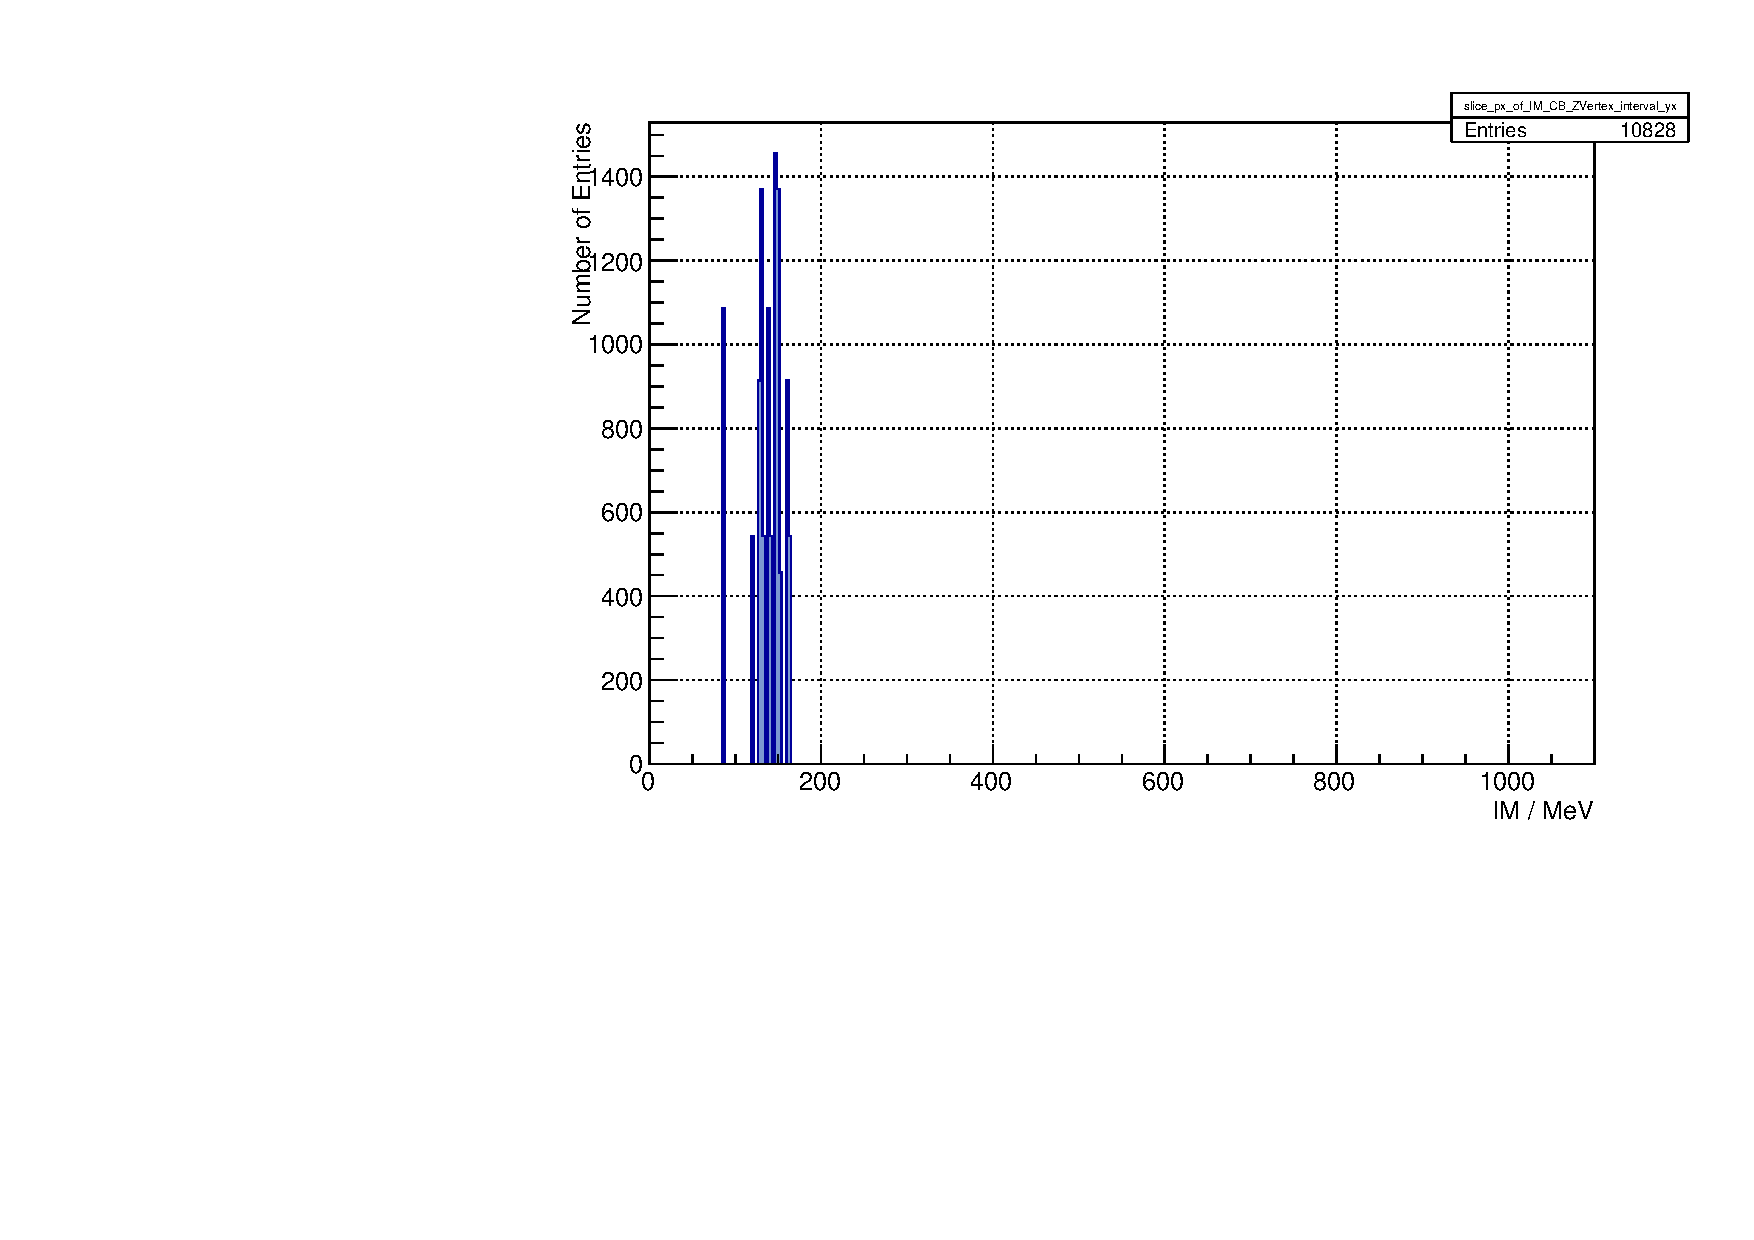
\includegraphics[width=74mm]{20171104BadRandomGenerator}


		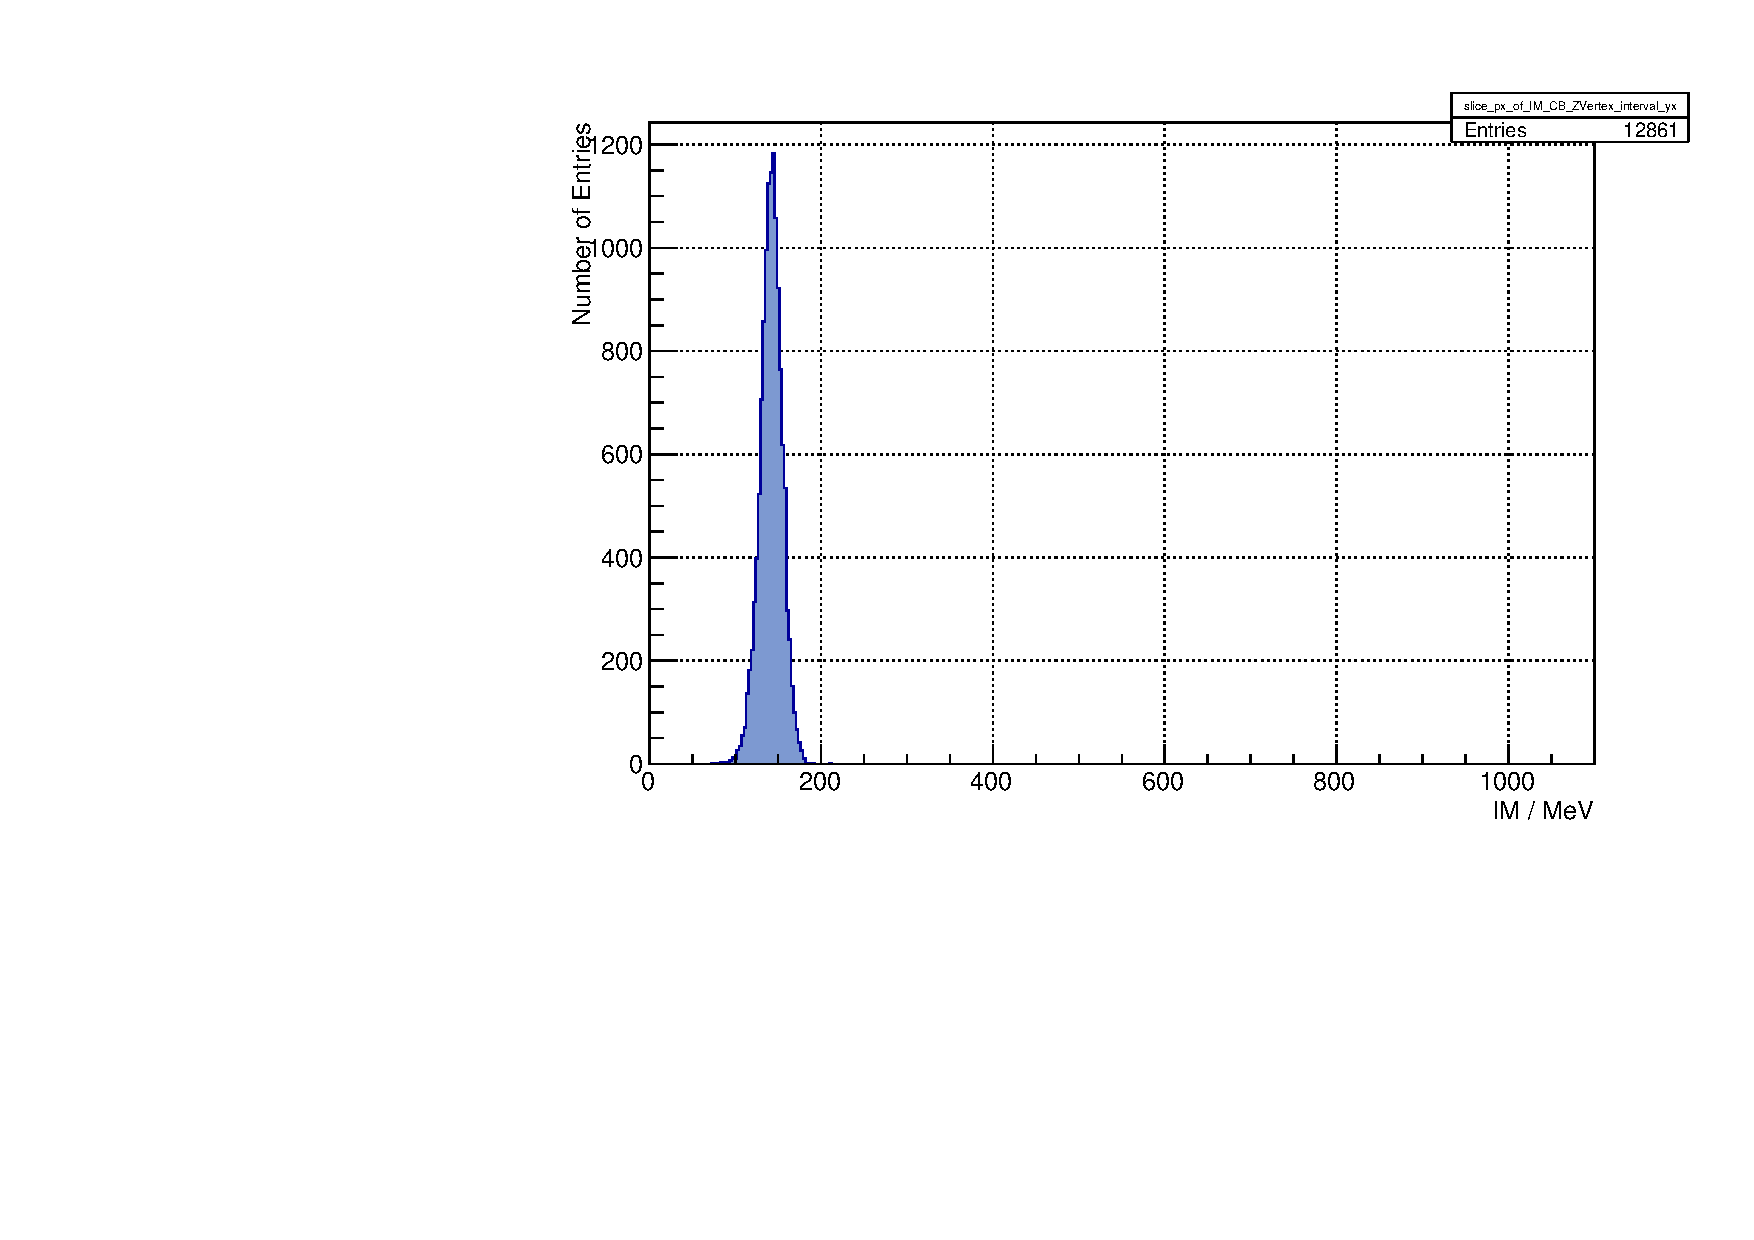
\includegraphics[width=74mm]{20171204GoodRandomGenerator}
	\end{array}$
\end{center}
	\caption[Simulation: Beispiel f\"ur die Verteilung durch Zufallsgeneratoren]{Daten aus der Simulation: Beispiele f\"ur durch den Ereignisgenerator generierte Verteilungen. Links wird das Paket TRandom und rechts TRandom3 benutzt. Man erkennt direkt eine deutliche Verbesserung der Verteilung von TRandom auf TRandom3. Es handelt sich dabei jeweils um das Histogramm f\"ur Photonen mit einer Energie von $375\, \text{MeV}$ bis $400\,\text{MeV}$. Die Energie der beiden Photonen musste \"ahnlich sein.}
	\label{fig:Random-Verteilung}
\end{figure}



Folglich musste er ausgetauscht und durch den ebenfalls von ROOT bereitgestellten Zufallsgenerator namens TRandom3 ersetzt werden. Dieser besitzt mit $10^{6000}$ eine deutlich höhere Periodizität als TRandom. Zwar ben\"otigt er mit $45 \,\text{ns}$ pro gew\"urfelter Zahl etwas mehr Zeit, daf\"ur entspricht die Verteilung mehr der erwarteten. Zu sehen ist dies rechts in der Abbildung.

Schlie{\ss}lich muss noch überprüft werden, ob der neue Ereignisgenerator so wie der alte funktioniert. Dazu wird auch der alte Ereignisgenerator so eingestellt, dass die Energieverteilung des eintreffenden Photonenstrahls homogen im Interval von $1580\,\text{MeV}$ bis $1604\,\text{MeV}$ verteilt ist. Dadurch ist ein einfacherer Vergleich m\"oglich. 
%die Form der Verteilung der neuen $\pi^0$-Gun, der alten entsprach. Dazu wird die alte Gun ebenfalls so eingestellt, dass die Energieverteilung des eintreffenden Photonenstrahls homogen verteilt ist, dadurch ist ein einfacherer Vergleich möglich. 

\begin{figure}[h!]
\begin{center}
	
$\begin{array}{cc}

		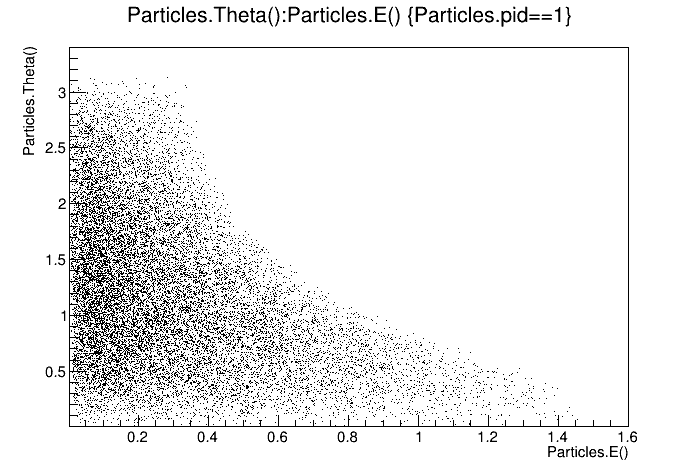
\includegraphics[width=74mm]{New_MC_Pi0_Gun/20170704Pi0_Gun_New}


		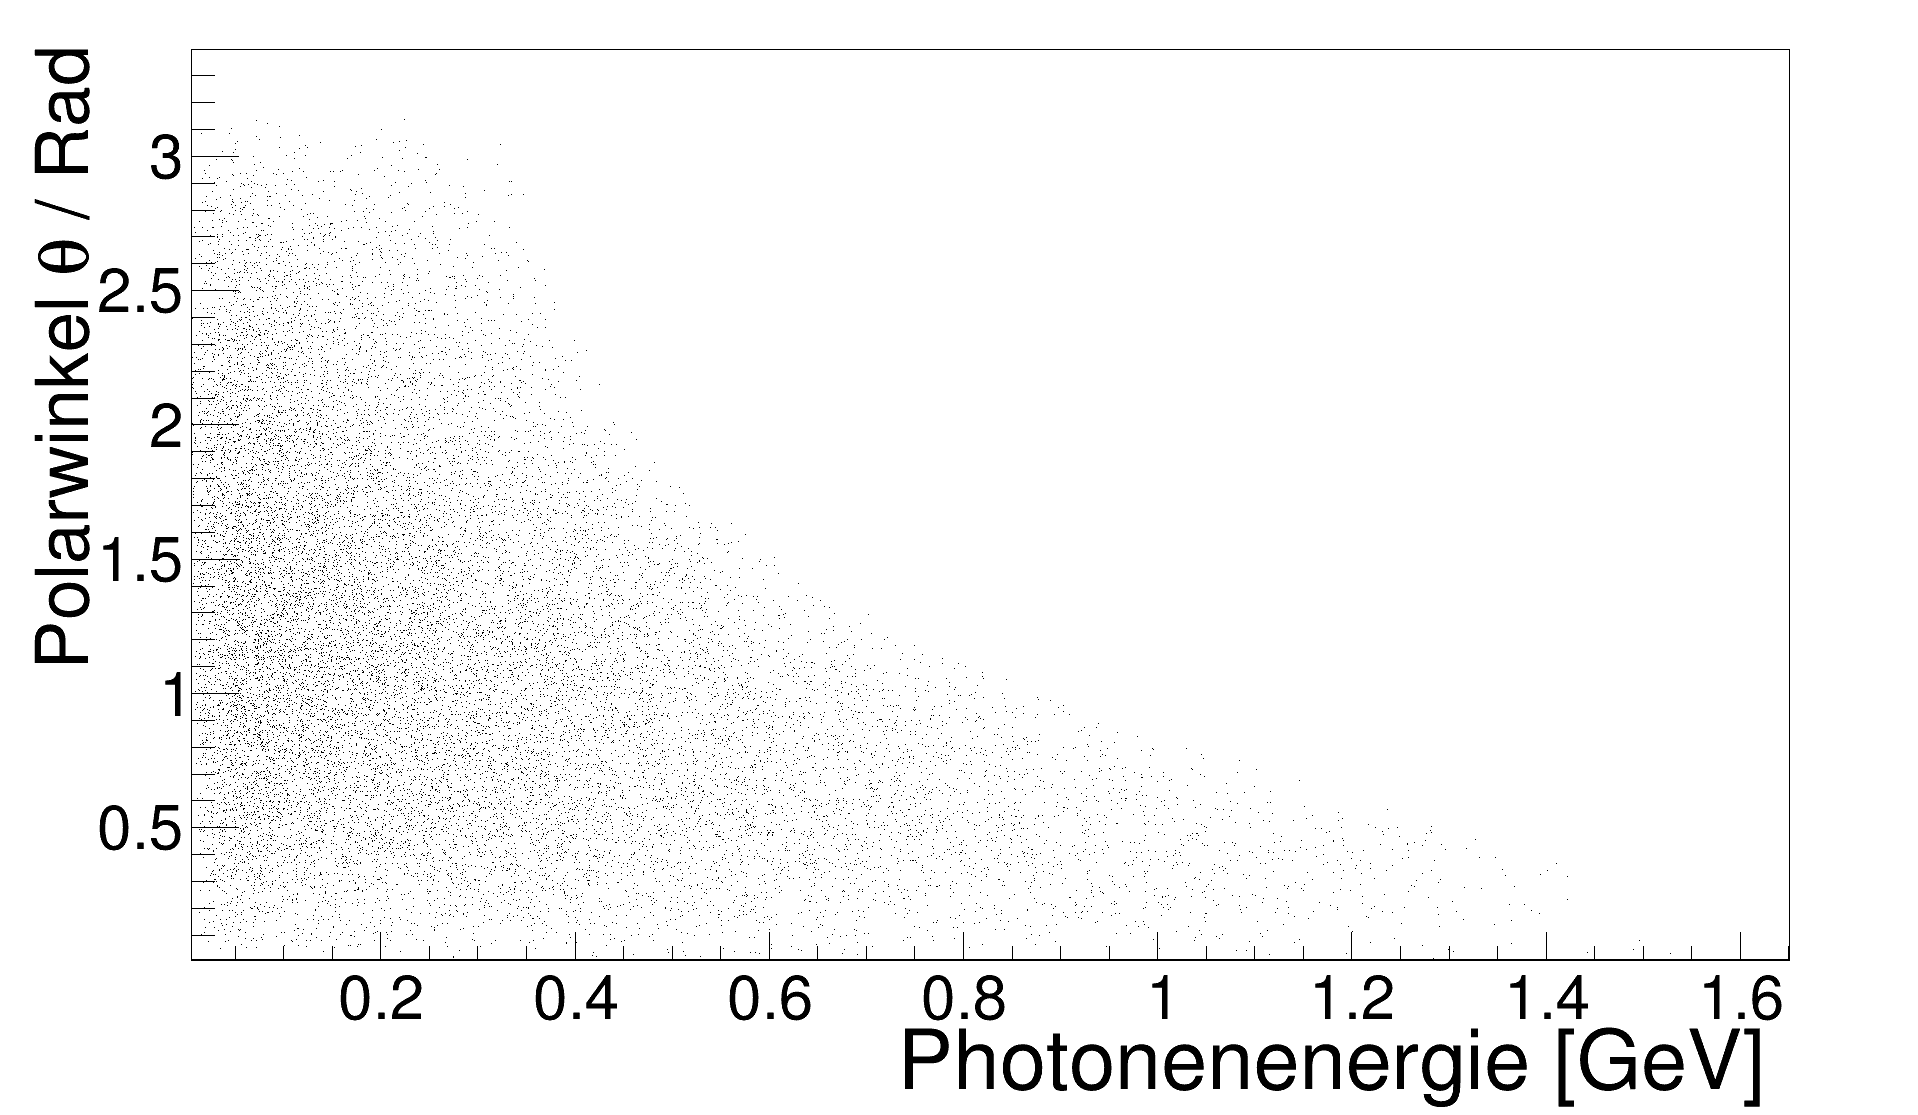
\includegraphics[width=74mm]{New_MC_Pi0_Gun/20170704Pi0_Gun_Old}
\end{array}$
\end{center}
	
	\caption[Simulation: Vergleich der Ereignisgeneratoren]{Links wird der neue und rechts der alte Ereignisgenerator benutzt. Aufgetragen ist der $\theta$-Winkel gegen die Energie der durch den Zerfall ausgesandten Photonen. Die beiden Pakete beinhalten jeweils $10^5\,\, \text{Ereignisse}$.}
	\label{fig:Vergleich-der-beiden-Guns}
\end{figure}

In den Plots von Abbildung \ref{fig:Vergleich-der-beiden-Guns} ist der $\theta$-Winkel der durch den $\pi^0$-Zerfall ausgesandten Photonen gegen ihre Energie aufgetragen. Links wird der neue und rechts der alte Ereignisgenerator benutzt.
Man erkennt, dass sich die Verteilung sehr stark \"ahneln, was darauf hindeutet, dass beide Ereignisgeneratoren gleich funktionieren.

Als letzte Absicherung wird aus den im Ereignisgenerator bestimmten Werten f\"ur die Energie der Photonen und ihrem \"Offnungswinkel die invariante Masse des $\pi^0$ berechnet. Zu sehen ist das in Abbildung \ref{fig:Direkte-Berechnung-der-PI-Masse}.

\begin{figure}[h!]
	\centering

		\centering
		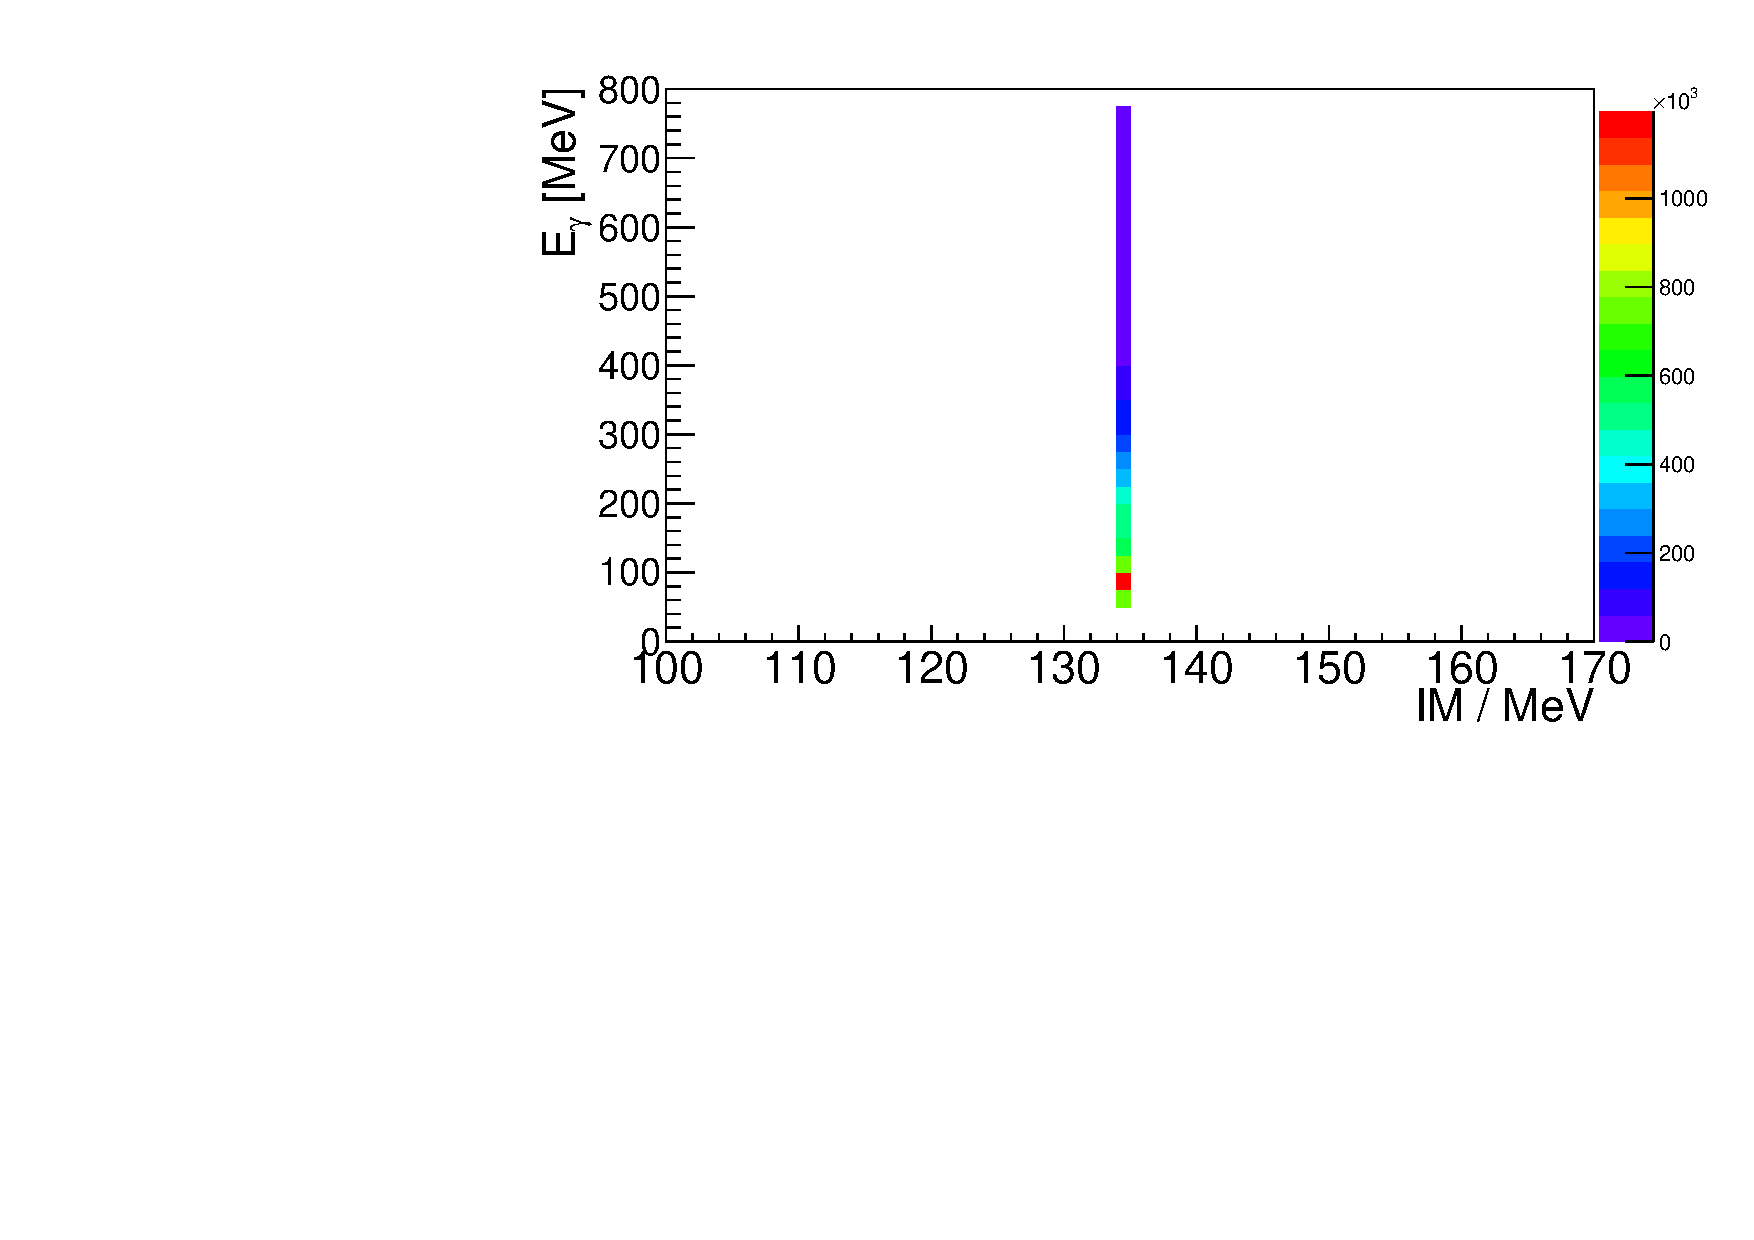
\includegraphics[width=0.9\textwidth]{20172504MCTrueME1}
		\caption[Ereignisgenerator: Direkte Berechnung der $\pi^0$-Masse]{Daten aus dem neuen Ereignisgenerator: Direkte Berechnung der $\pi^0$-Masse. Es werden nur Photonen mit einer \"ahnlichen Energie betrachtet.}
		\label{fig:Direkte-Berechnung-der-PI-Masse}

\end{figure}

Wie zu erwarten war, liegt keine Abweichung vor, wenn man mit den Daten aus dem Ereignisgenerator direkt die $\pi^0$-Masse berechnet, da hier die Detektoraufl\"osung noch nicht beitragen hat.

Also kann angenommen werden, dass der neue $\pi^0$-Ereignisgenerator wie gewünscht funktioniert.



%Nach einer gr\"o{\ss}eren Simulation mit 1000 Paketen, welche jeweils 10000 Prozesse beinhalteten, insgesamt also 10 Millionen Prozesse, stellte sich allerdings heraus, dass die Verteilung der Ereignisse nicht wie erwartet war.








\chapter{Studien zur Kalibrierung des Crystal-Ball}
\label{chap:Studien}

Zerf\"allt ein $\pi^0$, so werden nach Reaktion \ref{eq.pi0decay} zwei Photonen frei. Diese Photonen werden an der A2 durch den Crystal-Ball Detektor nachgewiesen. Dabei wird, sowohl der Winkel zwischen den beiden Photonen, als auch die Energie der Photonen bestimmt, um die invariante Masse des $\pi^0$ ausrechnen zu k\"onnen.
\newline

Eine Kalibration ist notwendig, um zu einem gegebenen Wert einen Umrechnungsfaktor zu bestimmen, der die gemessene Ladung in physikalisch aussagekr\"aftige Werte, zum Beispiel MeV oder ns, umrechnet. Diese Umrechnungsfaktoren m\"ussen f\"ur jeden Detektorkristall einzeln bestimmt werden, um die durch den experimentellen Aufbau bedingten Unterschiede ausgleichen zu können \cite{Un08}.



\section{Strahlzeit}
\label{sec:Reelle-Daten}

Im folgenden Abschnitt werden die gemessenen Daten aus der Strahlzeit Oktober 2014 verwendet. Die Strahlenergie betr\"agt $1604 \,\text{MeV}$. Die Energie des Photonenstrahls betr\"agt $1420\,\text{MeV}$ bis $1580\,\text{MeV}$, welche durch den End-Point-Tagger bestimmt wird. 

\subsection{Energie Abhängigkeit}
\label{sec:Energie-Interval-Abhaengigkeit}

Als erstes wird überprüft, ob eine Abhängigkeit der Kalibrierung im Bereich verschiedener Energieintervalle vorliegt. Sprich, stimmt die Kalibrierung auch dann noch, wenn die Energie der beiden detektierten Photonen sich ähnelte. Das hei{\ss}t, es werden Photonenpaare ausgew\"ahlt, deren Energie sich maximal um $25 \,\text{MeV}$ unterscheidet. Diese Bedingung wird eingef\"uhrt, da man auf diese Weise herausfinden kann, ob die Kalibrierung auch noch f\"ur zum Beispiel zwei hoch energetische Photonen stimmt, da man wei{\ss}, dass beide Photonen eine hohe Energie besitzen. Anders kann die Folgerung nicht getroffen werden, da man sonst eine \textit{Mischung} der Energien hat und man nicht sagen kann, welcher Effekt durch welche Energie verursacht wird.

Deswegen werden im kompletten Kapitel \ref{chap:Studien} nur Photonen mit dieser maximalen Energiedifferenz betrachtet.

Zur Untersuchung k\"onnen dann aus den Daten der Strahlzeit, die invariante Masse des $\pi^0$ mit folgender Gleichung berechnet werden.

 \begin{equation}
 \begin{split}
 {m_{\text{rec}}=\sqrt{2E_1E_2(1-\cos(\alpha))}}
 \label{eq:Formel-zur-Berechnung-der-invarianten-Masse}
 \end{split}
 \end{equation}

Hier ist $m_{\text{rec}}$ die berechnete Masse aus den beiden Energien $E_1$ und $E_2$ der Photonen. $\alpha$ ist der \"Offnungswinkel zwischen den beiden Photonen. Um diesen zu berechnen muss angenommen werden, dass das Pion im Ursprung zerf\"allt. Mehr dazu in Abschnitt \ref{sec:Z-Vertex-Abhaengigkeit}.
Die Herleitung der Gleichung \ref{eq:Formel-zur-Berechnung-der-invarianten-Masse} befindet sich im Anhang \ref{sec:Herleitung-der-Formel-zur-Berechnung-der-invarianten-Masse}.

Mit diesen Daten kann schließlich ein zweidimensionales Histogramm mit der invarianten Masse auf der x-Achse angelegt werden. Auf der y-Achse ist die Energie der Photonen aufgetragen, welche in Intervalle mit einer Breite von $25 \,\text{MeV}$ unterteilt ist. 


\begin{figure}[h!]
	\begin{center}
		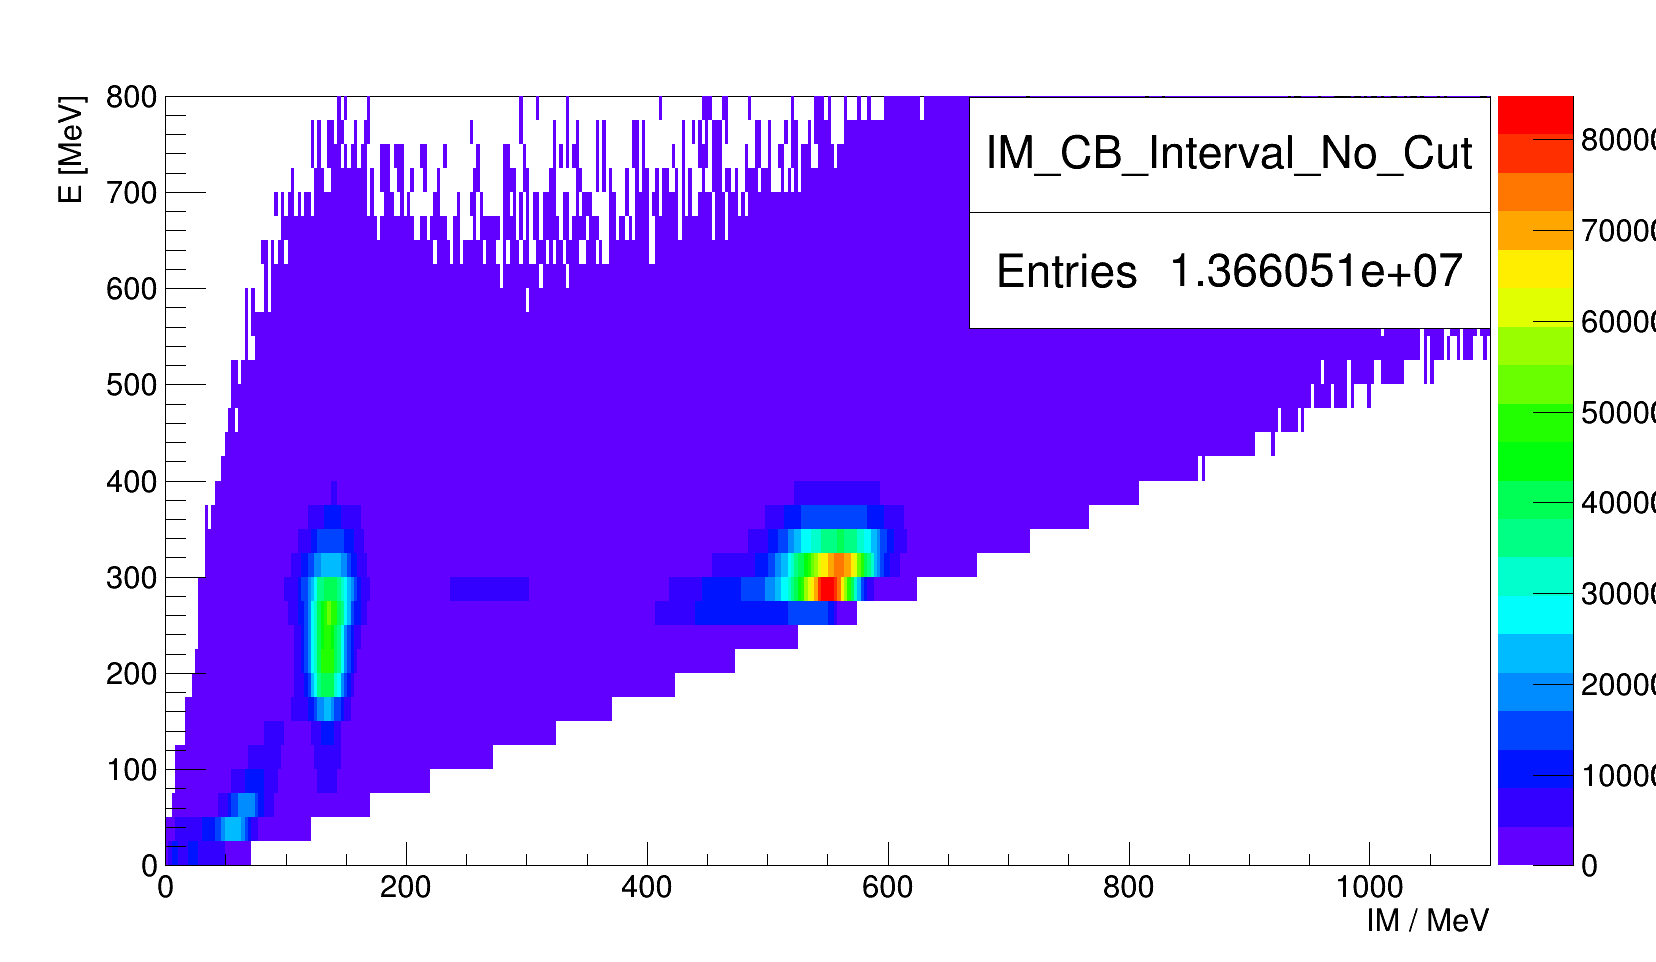
\includegraphics[width=100mm]{NewCalib/Strahlzeit2014/20171904Uncharged2DHist}
	
		\caption[Strahlzeit: 2D-Histogramm; Keine weiteren Bedingungen]{Daten aus der Strahlzeit: Auf der x-Achse ist die errechnete invariante Masse aufgetragen, die y-Achse ist in $25 \,\text{MeV}$ Intervalle aufgeteilt. Es werden nur Photonen ber\"ucksichtigt, die sich energetisch ähneln. Das hei{\ss}t ihre Energie unterscheidet sich maximal um $25 \,\text{MeV}$.}
			\label{fig:Energy-Interval-Hist-All-Bins}
	\end{center}
\end{figure}

Beim Füllen des Histogramms wird darauf geachtet, dass sich die Energien der beiden Photonen um maximal $25 \,\text{MeV}$ unterscheiden.

Im folgenden werden nur die Energieintervalle f\"ur Photonen von $125 \,\text{MeV}$ bis $450\, \text{MeV}$ ber\"ucksichtigt.

Dieser Bereich ist bewusst gew\"ahlt, da f\"ur kleinere Energien der Peak des $\pi^0$ zu stark durch den Untergrund gest\"ort wird und somit die Position nicht eindeutig bestimmt werden kann. F\"ur Energien oberhalb von $450\,\text{MeV}$ liegen nicht mehr genug Ereignisse vor, sodass h\"ohere Energieintervalle ebenfalls verworfen werden m\"ussen. 


Um nun die Position des $\pi^0$ zu bestimmen, wird für jedes Intervall über einen bestimmten Bereich der errechneten invarianten Masse mit Hilfe von ROOT gefittet. Dieser Bereich ist unterschiedlich f\"ur verschiedene Photonenenergien. Betrachte dazu Abbildung \ref{fig:similarenergyallfitsuncharged}. Der $\pi^0$-Peak ist zum Beispiel f\"ur die Photonenenergie im Bereich von $125\, \text{MeV}$ bis $150 \,\text{MeV}$ noch relativ stark durch den Untergrund gest\"ort, wodurch sein Fitintervall kleiner gew\"ahlt werden muss. F\"ur gro{\ss}e Photonenenergien verbreitert sich der $\pi^0$-Peak. Folglich muss hier das Intervall gr\"o{\ss}er gew\"ahlt werden. Als Fitfunktion wird die Crystal-Ball-Funktion (Kapitel \ref{sec:CB-Funktion}) verwendet. 
Aus diesen Fitdaten kann dann die Position des $\pi^0$ bestimmt werden.



  % Sein Peak wird allerdings sehr stark durch den Untergrund gest\"ort. Der Fokus dieser Arbeit lag zwar bei der Betrachtung des $\pi^0$, allerdings war es auch interresant die Position des $\eta$-Peaks zu betrachten, daher wurde nach einem Weg gesucht, den Untergrund m\"oglichst stark zu reduzieren. 
  
 %Daher wurde nun auch \"uberpr\"uft, ob die detektierten Teilchen eine Ladung besa{\ss}en, wenn ja, dann handelte es sich nicht um Photonen und sie wurden nicht in das Histogramm eingef\"ugt. 
 
%\begin{figure}[h!]
%\centering
%\begin{minipage}{0.45\textwidth}
%	\centering
%		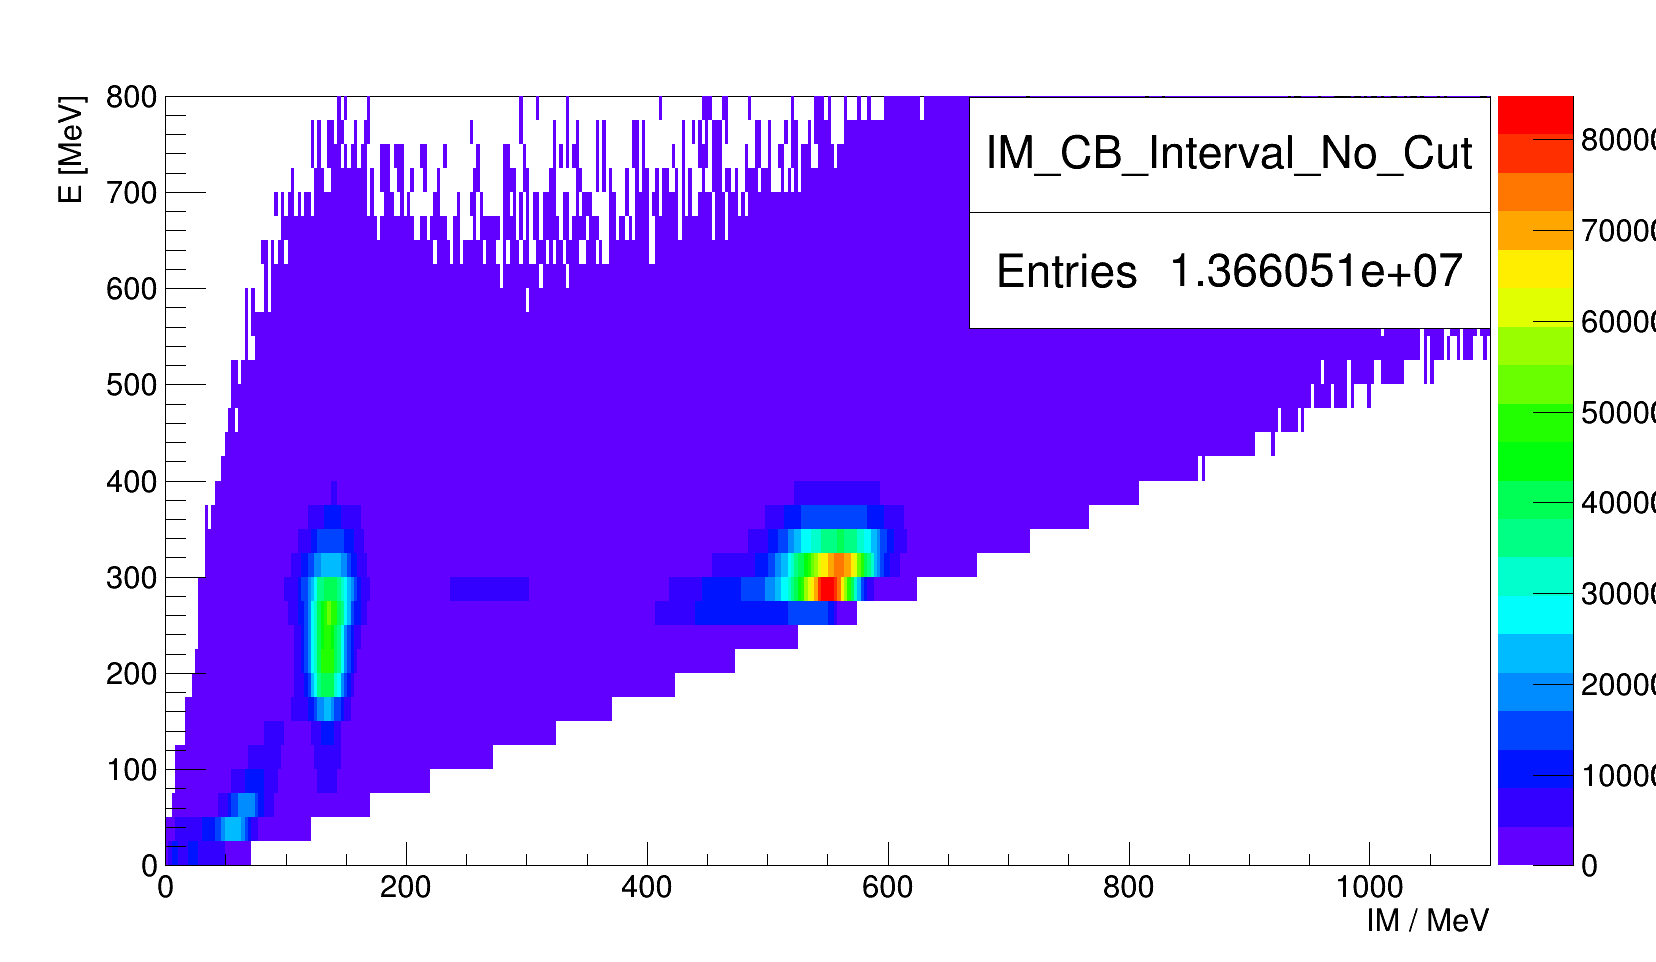
\includegraphics[width=0.9\textwidth]{NewCalib/Strahlzeit2014/20171904Uncharged2DHist}
%		
%		\label{fig:Symmetric-Uncharged-Hist-No-Cut}
%\end{minipage}
%\hfill
%\begin{minipage}{0.45\textwidth}
%	\centering
%	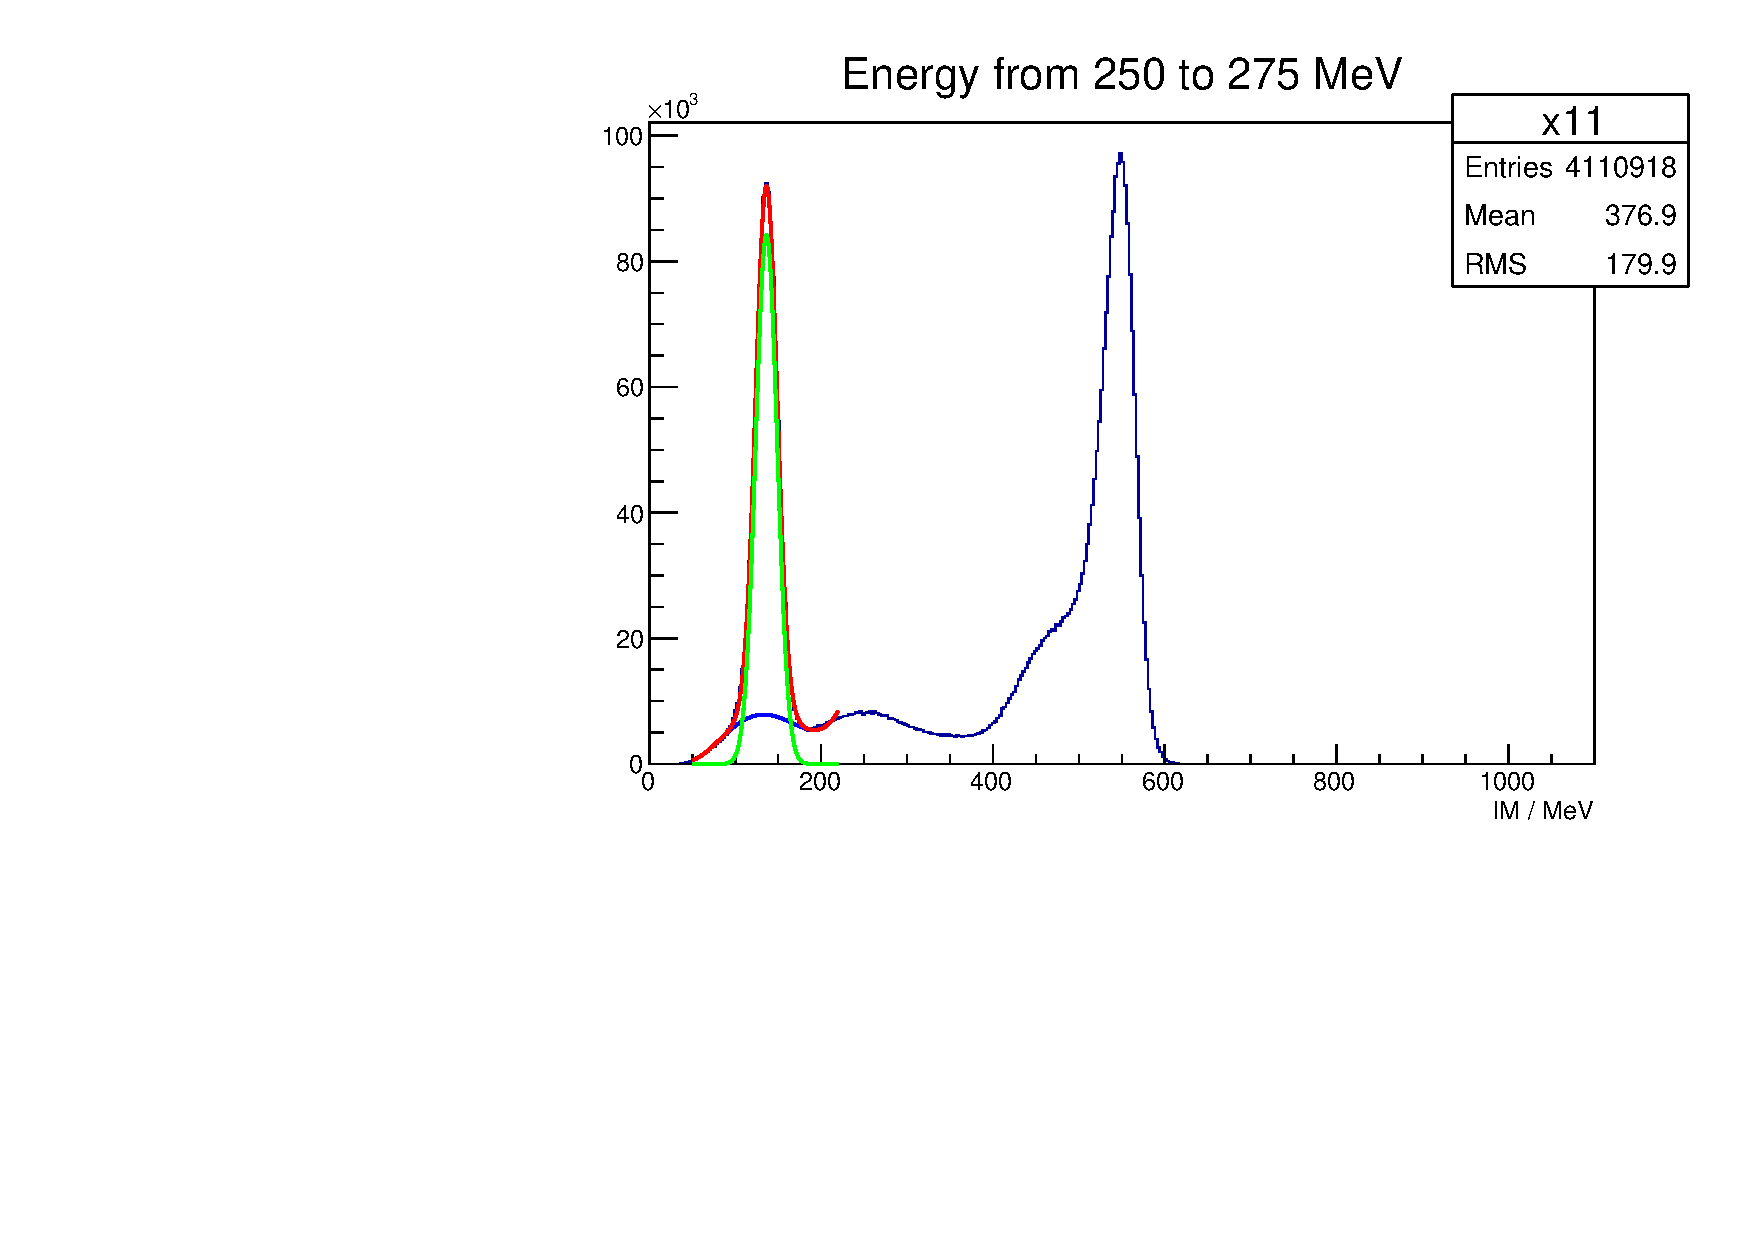
\includegraphics[width=0.9\textwidth]{NewCalib/Strahlzeit2014/20171904RealUnchargedFitExample}
%\end{minipage}
%\caption{Links ist das 2-D Histogramm zu sehen, f\"ur welches \"uberpr\"uft wurde, ob die gemessenen Teilchen ungelafen waren. Rechts ist ein Beispielfit aus diesem Historgramm mit der Crystal-Ball-Funktion zu sehen. Sowohl der $\pi^0$, als auch der $\eta$-Peak sind deutlich ausgepr\"agter.}
%\end{figure}
 
 %Bereits an diesem neuem Histogramm war zu erkennen, dass die St\"orung durch den Untergrund stark reduziert wurde, was einen besseren Fit f\"ur sowohl das $\pi^0$ als auch das $\eta$ erm\"oglichte. %Deswegen wurden nun, auch in den folgenden kapiteln, die Teilchen auch auf \"uberpr\"uft.
 
 %Nun wurde auch \"uber dieses Histogramm f\"ur das $\pi^0$ von 125 MeV bis 450 MeV gefittet.\\
 
 Um die Abweichung zwischen der rekonstruierten Masse und der $\pi^0$ Masse zu bestimmen wird folgende Gleichung angewandt.
 
 \begin{equation}
 A = (\frac{m_{\text{rec}}}{m_{\pi^0}}-1)
 \end{equation}
 
 Dabei ist $m_{\text{rec}}$ die rekonstruierte Masse und $m_{\pi^0}$ die tats\"achliche Masse. Die Abweichung $A$ gibt den Unterschied zwischen den beiden in Prozent an.
 
  %Daraus wird anschlie{\ss}end die Abweichung berechnet. Dazu wird die berechnete $\pi^0$-Peakposition durch den Literaturwert des $\pi^0$ geteilt. Anschlie{\ss}end wird noch Minus 1 gerechnet. Dieses Ergebnis wird mit 100 multipliziert, um die Abweichung in Prozent zu erhalten.
 
 \begin{figure}[h!]
 	\begin{center}
 		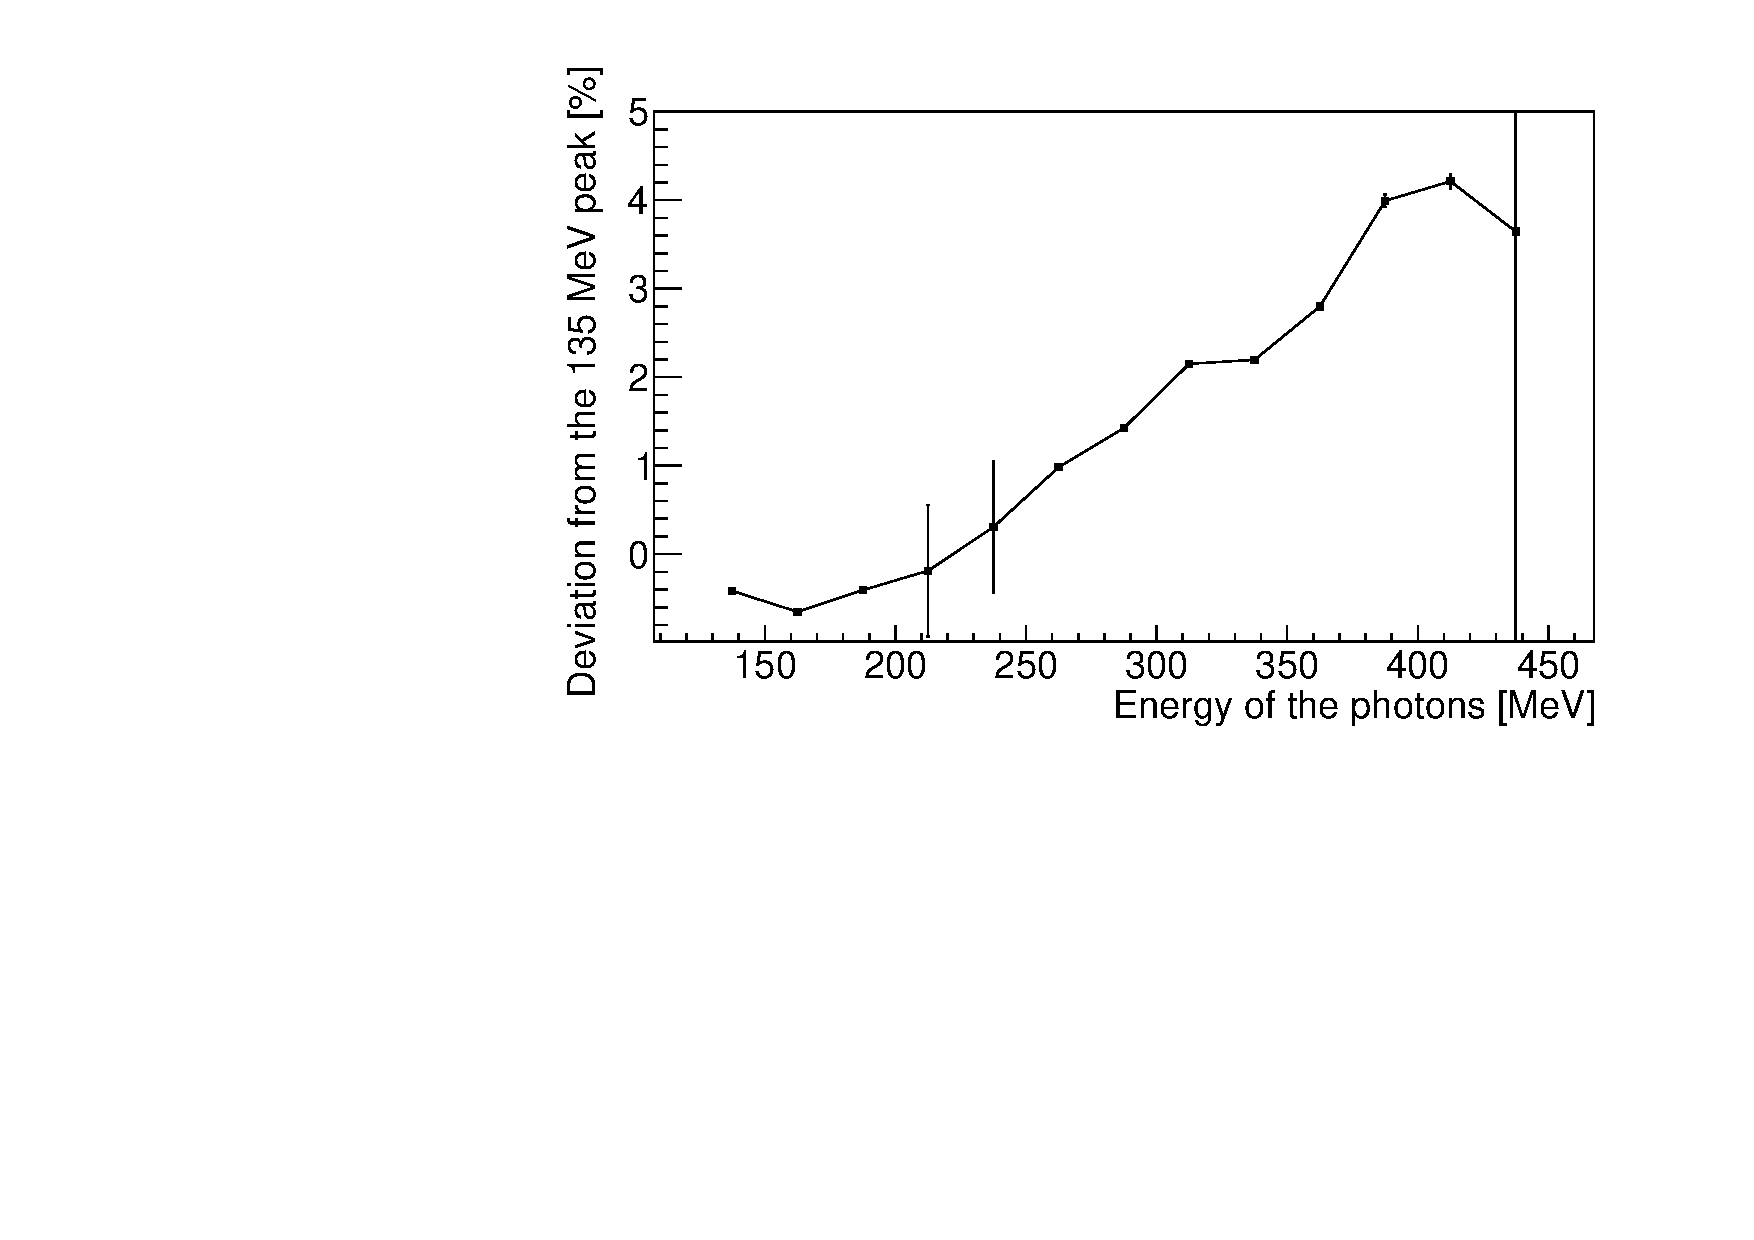
\includegraphics[width=100mm]{20170405StrahlzeitDeviatoinNoCut}
 	
 		\caption[Strahlzeit: Abweichung; keine weiteren Bedingungen]{Daten aus der Strahlzeit: Die Abweichung der errechneten Position des $\pi^0$ Peaks ist gegen die Energie der Photonen aufgetragen.
 			Es gilt die Bedingung, dass die Energie der Photonen sich \"ahneln muss. Alle Fits sind in Abbildung \ref{fig:similarenergyallfitsuncharged} zu sehen.} 
 		\label{fig.Energydependency_pion}
 	\end{center}
 \end{figure}

In Abbildung \ref{fig.Energydependency_pion} sind die errechneten Abweichungen der invarianten Masse des $\pi^0$ gegen die Energie der Photonen aufgetragen. Zu sehen ist eine deutliche Abweichung zum Literaturwert des $\pi^0$ Peaks für hohe Energien. 

F\"ur eine Photonenenergie von ungef\"ahr $125\,\text{MeV}$ liegt nur eine kleine Abweichung vor. Hier ist die errechnete Masse etwas zu klein. Allerdings \"andert sich die Abweichung bei steigender Photonenenergie mit einer \textit{Steigung} von ca. +1\% pro $50\,\text{MeV}$. Die maximale Abweichung wird bei einer Photonenenergie von $425\,\text{MeV}$ erreicht und betr\"agt etwas mehr als +4\%. Bei einer Photonenenergie von etwa $450\,\text{MeV}$ wird die Abweichung wieder etwas kleiner und betr\"agt nur etwas weniger als 4\%.
Auch fällt auf, dass die Abweichung größtenteils positiv ist. In der Regel wird also eine zu gro{\ss}e invariante Masse berechnet.

Daraus folgt, dass eine Abhängigkeit zwischen der Position des $\pi^0$-Peaks und der Energie der Photonen vorliegt. 



Die meisten Fehlerbalken sind so klein, dass sie in der Markierung der Punkte untergehen. Allerdings besitzen der vierte, f\"unfte und vor allem der letzte Wert auffallend große Fehlerbalken. Schaut man sich allerdings die drei Fits dazu genauer an, so kann man keinen wirklichen Grund für diese Größe feststellen.

 %Abbildung \ref{fig:Reduzierter-Untergrund-Fit} soll auch als Beispiel für einen funktionierenden Fit dienen. Da in dieser Arbeit noch sehr viel gefittet wird, und die Plots mit den Fits wenig aufschlussreich sind, wird auf die anderen Fits verzichtet, außer es handelt sich um einen Ausreißer, dann wird dieser Fit noch im Anhang abgebildet, um zu zeigen, dass er doch in Ordnung ist.

%Für eine Photonenenergie von ca. 150 MeV lag fast keine Abweichung vor. Diese Abweichung nahm allerdings im Intervall von 150 MeV bis 325 MeV konstant mit einer \textit{Steigung} von 1\% pro 50 MeV Photonenenergie zu. Ab 325 MeV nah, diese \textit{Steigung} zu und betrug im Intervall von 325 MeV bis 375 MeV ca. 2\% pro 50 MeV Photonenenergie. Schließlich flachte die Abweichung ab 375 MeV ab, und wurde sogar etwas kleiner. Die größte Abweichung lag mit über 7\% bei einer Photonenenergie von etwa 400 MeV vor.


%Daraufhin wurde das gleiche Verfahren nochmal angewendet, allerdings wurde dieses mal die Bedingung weggelassen, dass die Photonen sich energetisch ähneln mussten. Die Bedingung, dass die registrierten Teilchen ladungsfrei sein mussten, galt weiterhin. Die errechnete invariante Masse der Photonen wurde in das Histogramm (Abb.: \ref{fig:Energy-Intervall-Hist-All-Energys-No-Condition}) eingetragen. Die Energieintervalle wurden direkt mit der Crystal-Ball-Funktion gefittet. Zu sehen in Abbildung \ref{fig:allenergyallfits}. Nun wurden ebenfalls die errechneten invarianten Massen des $\pi^0$ gegen die Energien der Photonen aufgetragen (Abb.: \ref{fig:Energy-Intervall-No-Condition-Deviation-1303}). Auch hier war eine deutliche Abweichung der Position des $\pi^0$ zum Literaturwert zu erkennen. Diese Abweichungen betrugen zwar nur fast 2\% (siehe Abb. \ref{fig:Relative-Deviation-Energy-Interval-No-Condition}}), sind aber nicht vernachl\"assigbar. 

In den folgenden Abschnitten wird versucht, die Ursache für die in Abbildung \ref{fig.Energydependency_pion} gefundene Abweichung zu finden.


\subsection{Vernachl\"assigung der Detektoren am Rand}
\label{sec:Vernachlaessigung-der-Detektoren-am-Rand}

Als Ursprung der in Kapitel \ref{sec:Energie-Interval-Abhaengigkeit} ermittelten Abweichung wird zun\"achst der Aufbau des Crystal-Balls vermutet. Genauer gesagt, der Strahlenein- und -ausgang. Denn durch diese haben die Detektoren im Crystal-Ball nicht alle gleich viele Nachbardetektoren und da ein Photon seine gesamte Energie nicht an einen Detektorkristall abgibt, sondern immer auch an seine Nachbarn, k\"onnen diese Randdetektoren nicht ideal kalibriert werden und damit k\"onnen die Schauer am Rand nicht unverf\"alscht gemessen werden. 


%In erster Linie war es wichtig einen Vergleich zwischen der $\pi^0$ Position mit und ohne Ber\"ucksichtigung der Detektoren am Rand zu erhalten. Es sollte herausgefunden werden, ob so die Messung verbessert werden konnte. Zus\"atzlich galten, wie in Kapitel \ref{sec:Energie-Interval-Abhaengigkeit}, die Bedingungen, dass die Energie der Photonen sich im gleichem Energieinterval befand und dass die registrierten Teilchen ungeladen sein m\"ussen. 
%ohne die Bedingung, dass die Histogramme nur gef\"ullt werden d\"urfen, wenn sich die Energie der Photonen im gleichem Intervall befand. 

%\begin{figure}[h!]
%	\begin{center}
%		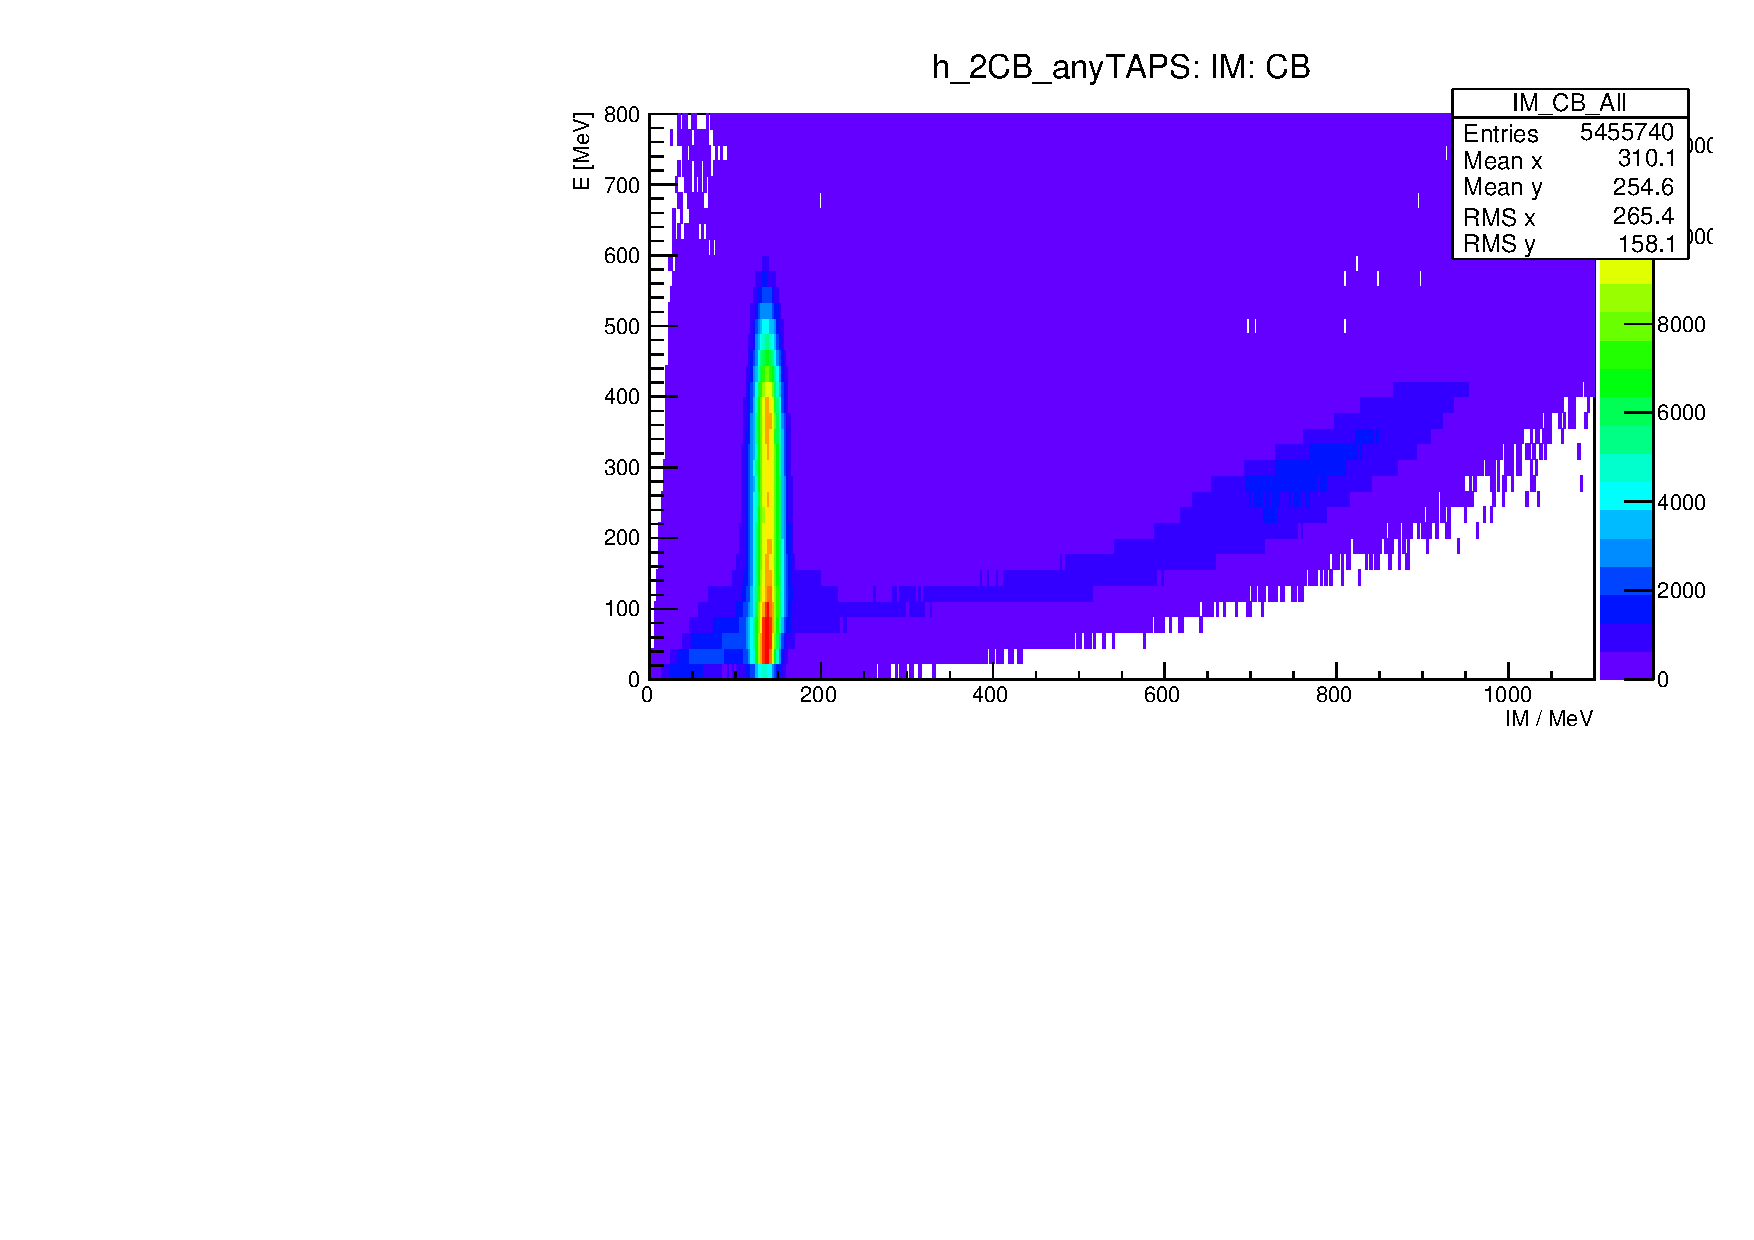
\includegraphics[width=100mm]{EnergyAngle2DHistoNoEdgePi0Position1403}
%		\caption{2-D Histogramm: Auf der x-Achse ist die errechnete invariante Masse und auf der y-Achse ist der Energie der Photonen aufgetragen. Die y-Achse ist in Energieintervalle der Breite 25 MeV unterteilt}
%		\label{fig:2D-Hist-Angle-Energy-Position-Pi0}
%	\end{center}
%\end{figure}

%Das gef\"ullte Histogramm ist in Abbildung \ref{fig:2D-Hist-Angle-Energy-Position-Pi0} zu sehen. Hier erkennt man auch direkt, dass simulierte Daten benutzt wurden, da der $\pi^0$-Peak viel st\"arker ausgepr\"agt war, im Vergleich zu den reellen Daten.

Zus\"atzlich zu den in Kapitel \ref{sec:Energie-Interval-Abhaengigkeit} geltenden Bedingungen wird noch die Bedingung hinzugef\"ugt, dass die Detektoren am Rand des Strahlenein- und -ausgangs nicht betrachtet werden. Dies erreicht man dadurch, dass alle Reaktionen, die ein oder mehrere Photonen besitzen, welche einen Winkel von 30$^{\circ}$ oder weniger zur Strahlenachse haben, verwerfen werden. Diese Gradzahl wurde durch eine grobe Absch\"atzung errechnet. Die \"Offnungen f\"ur den Strahlenein- und -ausgang haben einen Radius von 2 Detektoren, und erstrecken sich \"uber einen Polarwinkel von ca. 20$^{\circ}$. Folglich h\"atte ein Ring aus Detektoren um diese \"Offnungen einen Polarwinkel von 10$^{\circ}$. 
 
Auch f\"ur diese Bedingung wird anschlie{\ss}end ein Histogramm angelegt (Abb.: \ref{fig:30-Degree-Cut-Histogramm}) und über die einzelnen Photonenenergieintervalle wird gefittet (Abb.: \ref{fig:30-Degree-Cut-RealData-All-Fits}), um die Position des $\pi^0$ zu bestimmen. Das Energieintervall, das betrachtet und gefittet wird, entspricht dem aus Kapitel \ref{sec:Energie-Interval-Abhaengigkeit}, damit ist ein besserer Vergleich zwischen den verschiedenen Effekte m\"oglich.

Zum besseren Vergleich der beiden Ergebnisse werden die relative Abweichungen mit und ohne Bedingung zusammen in einen Graphen gezeichnet.
\begin{figure}[h!]
	\begin{center}
		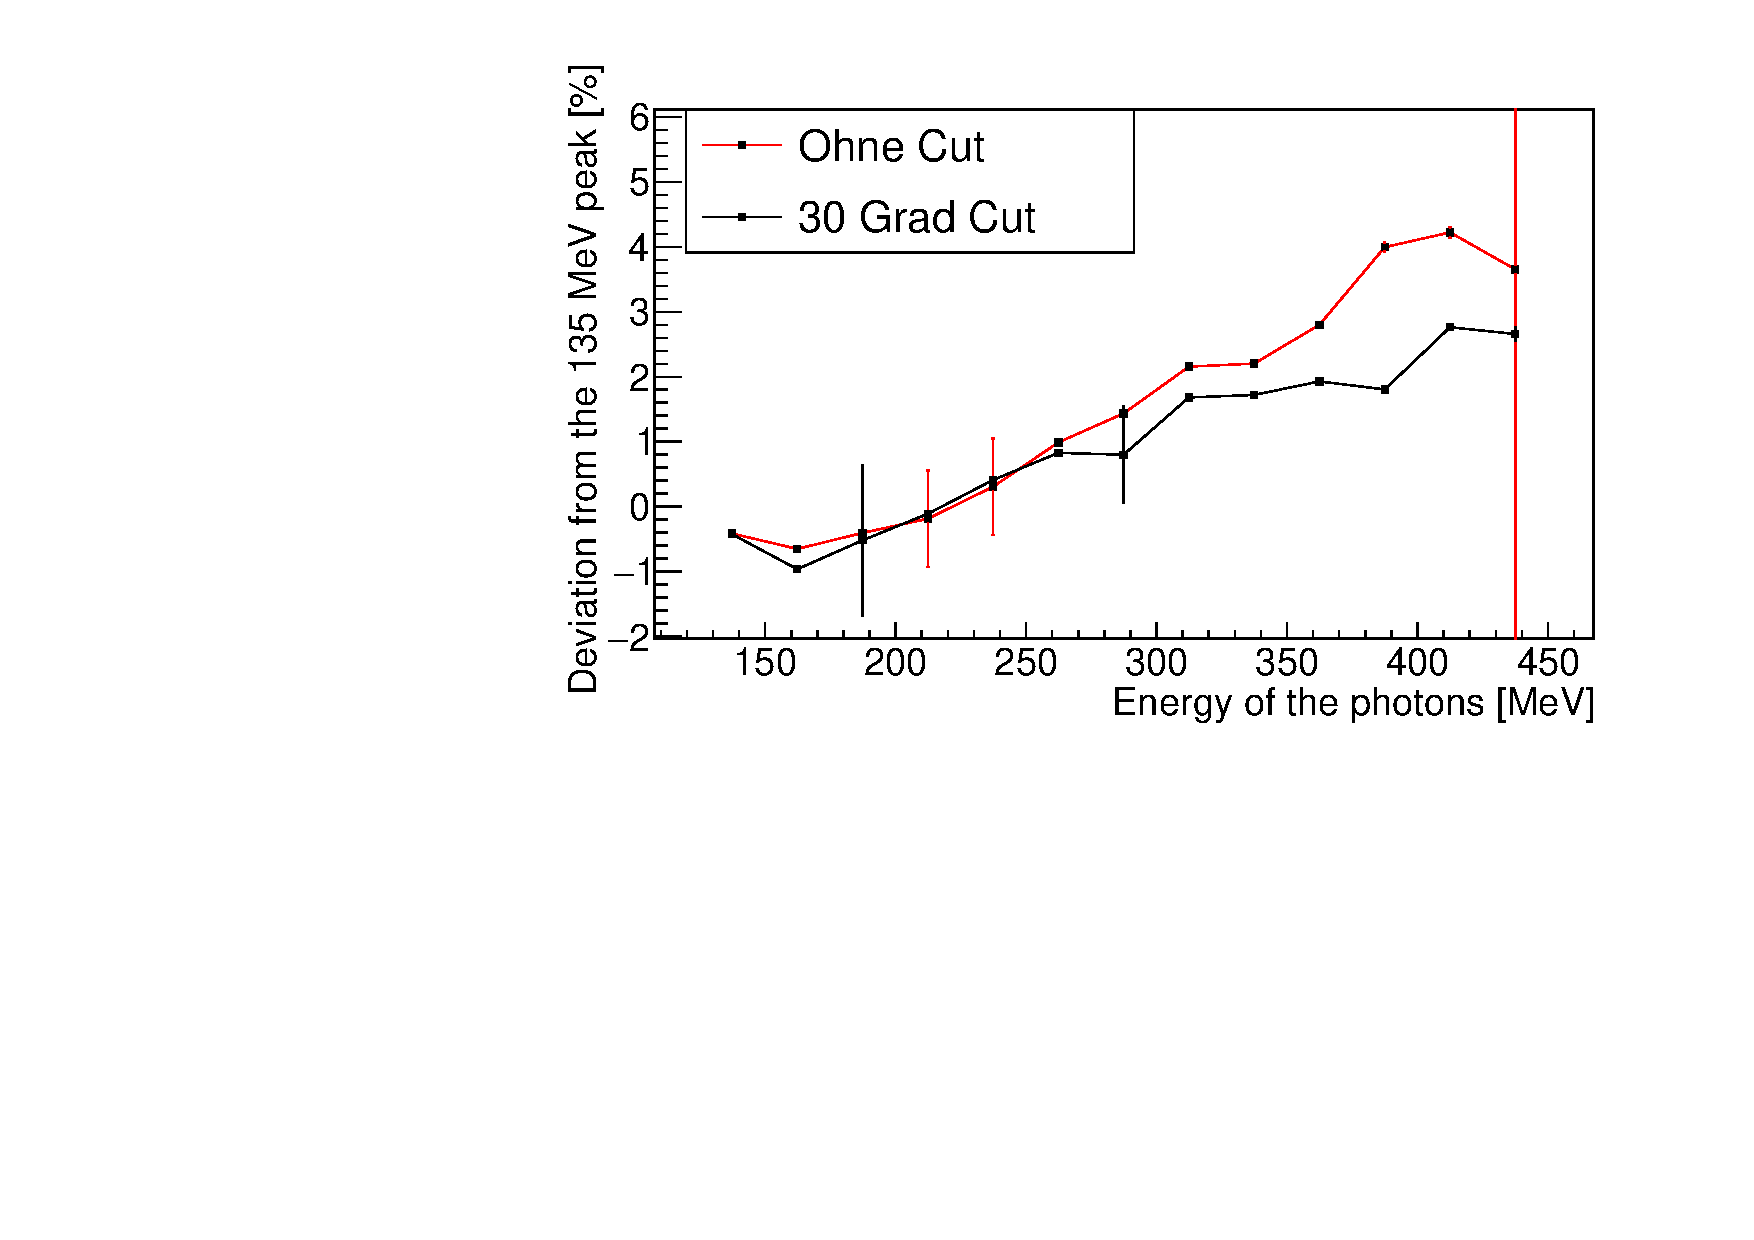
\includegraphics[width=100mm]{20170405StrahlzeitBothDeviation}
		\caption[Strahlzeit: Vernachl\"assigung der Detektoren am Rand; Abweichung]{Daten aus der Strahlzeit: Die Abweichung der errechneten Position des $\pi^0$ Peaks ist gegen die Energie der Photonen aufgetragen. Die rote Linie stellt die relative Abweichung ohne die Bedingung, dass Photonen mit einem Winkel kleiner als 30$^{\circ}$ verworfen werden, die schwarze Linie mit der Bedingung. Die detektierten Photonen m\"ussen sich energetisch \"ahneln. Alle Fits sind in Abbildung \ref{fig:30-Degree-Cut-RealData-All-Fits} zu sehen.}
		\label{fig:Vernachlaessigung-Detektoren-am-Rand}
	\end{center}
\end{figure}

 

In der Abbildung \ref{fig:Vernachlaessigung-Detektoren-am-Rand} erkennt man, dass der Unterschied der beiden Betrachtungen f\"ur Photonenenergien unterhalb von $275\,\text{MeV}$ nur sehr klein ist. Bei einem so kleinen Unterschied kann man nicht mit Gewissheit sagen, dass der Schnitt bei 30$^{\circ}$ eine Verbesserung der $\pi^0$-Peak Position bewirkt hat. Die Differenz ist noch im Bereich der statistischen Fluktuation. 

F\"ur Photonenenergien oberhalb von ca. $ 275\,\text{MeV}$ ist eine deutliche Verbesserung der Abweichung zu erkennen. So liegt bei einer Photonenenergie von $400\,\text{MeV}$ mit Detektoren am Rand eine Abweichung der errechneten $\pi^0$-Peakposition zur invarianten Masse des $\pi^0$ von ungefähr 4\% vor, w\"ahrend die Abweichung bei gleicher Photonenenergie ohne Detektoren am Rand nur rund 2,5\% betr\"agt. 

Auch hier gibt es wieder Fehlerbalken, die auffallend gro{\ss} sind. Betrachtet man sich allerdings auch hier die jeweiligen Fits dazu, kann die Gr\"o{\ss}e der Fehlerbalken auch hier nicht nachvollzogen werden.

Ein vermuteter Grund, warum es nur eine Verbesserung für hohe Energien gibt, ist, dass hochenergetische Photonen dann erzeugt werden, wenn auch das Pion eine hohe kinetische Energie besitzt. Diese Photonen haben dann eine gr\"o{\ss}ere Wahrscheinlichkeit in Richtung des Strahlenausgang des Crystal-Balls aufzutreten.

Um das zu erkl\"aren betrachtet man zun\"achst ein ruhendes $\pi^0$. Dieses zerf\"allt in 2 Photonen in zuf\"alliger Richtung mit einem Winkel von 180$^{\circ}$ zueinander und mit einer Energie von jeweils $\nicefrac{m_{\pi^0}}{2} \approx67,5\, \text{MeV}$.

Gibt man dem $\pi^0$ nun einen Boost in $z$-Richtung, so erhalten auch die beiden Photonen einen Boost in diese Richtung.
Zur Veranschaulichung betrachtet man nun zwei extreme Beispiele:

\begin{enumerate}
	\item Im Ruhesystem des $\pi^0$ werden die Photonen in einem Winkel von 90$^{\circ}$ zur Strahlenachse ausgesandt. Wird nun ein Boost in $z$-Richtung angewandt, so erhalten beide Photonen einen gleich gro{\ss}en Impuls in $z$-Richtung und haben folglich beide die gleiche Energie und den gleichen Winkel zur $z$-Achse. Dieser Winkel wird kleiner, wenn der Boost st\"arker wird.
	\item Werden die Photonen allerdings entlang der $z$-Achse ausgesandt, so bewirkt ein Boost in $z$-Richtung nun, dass das Photon in $z$-Richtung Energie dazu erh\"alt, w\"ahrend das Photon entgegengesetzt zur $z$-Richtung Energie \textit{verliert}. Die Energiedifferenz nimmt also zu.
\end{enumerate}

F\"ur h\"ohere Photonenenergien werden diese Effekte verst\"arkt und alles in allem werden mehr Photonen in Strahlrichtung gemessen. Daraus folgt, dass Photonen mit niedriger Energie sich eher gleichm\"a{\ss}ig im Raum verteilen, w\"ahrend hochenergetische Photonen h\"aufiger am Strahlausgang des Crystal-Balls auftreten. Beachte, dass die hier betrachteten Photonen eine ähnliche Energie besitzen müssen.

Dies f\"uhrt auch zu einem weiteren Problem. Dadurch, dass die h\"oher energetischen Photonen wahrscheinlicher am Strahlenausgang vorliegen, werden nicht alle Detektoren im Crystal-Ball gleich ber\"ucksichtigt. So liegen, am Strahleneingang fast keine hochenergetische Photonen vor.


\begin{figure}[h!]
\begin{center}
	$\begin{array}{cc}
		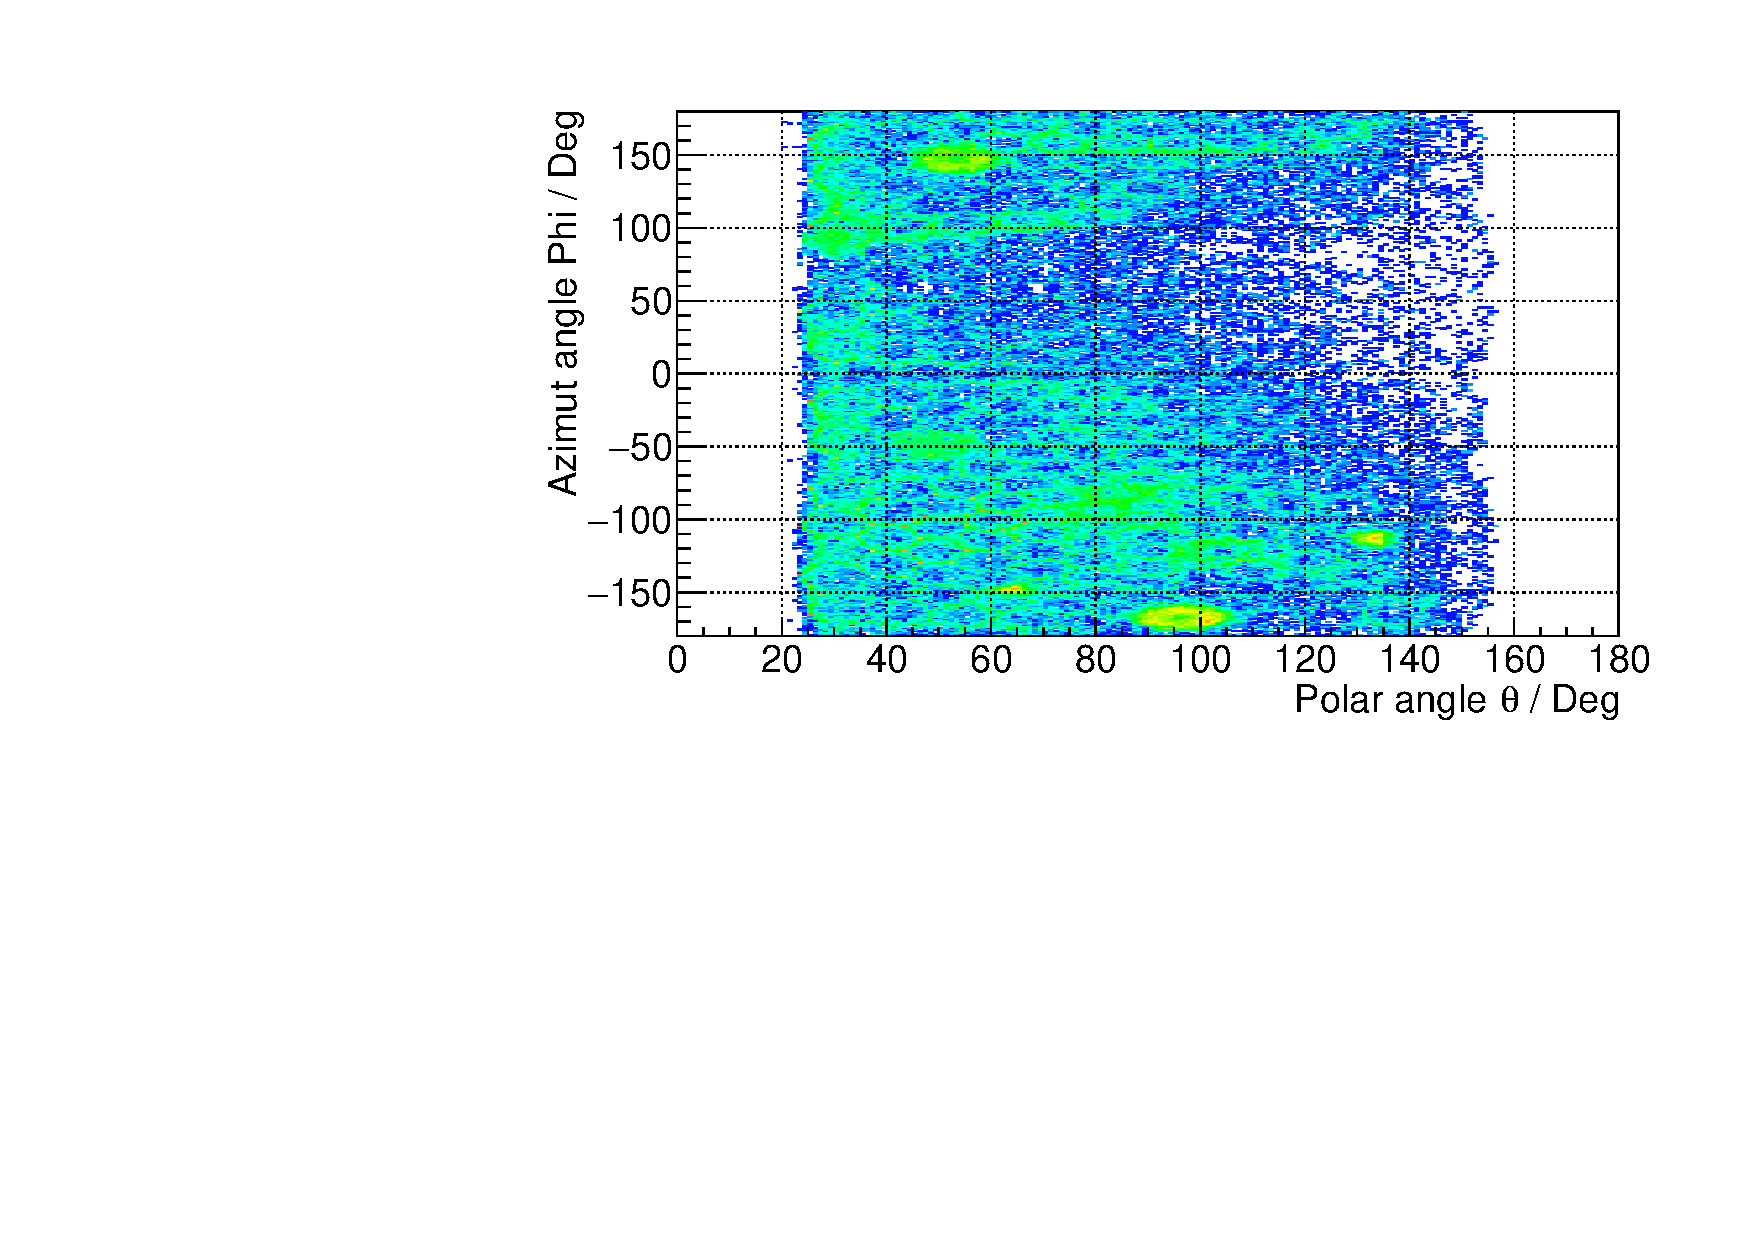
\includegraphics[width=74mm]{20170504ThetaPhiEnergySymmetric2014_10_125}

		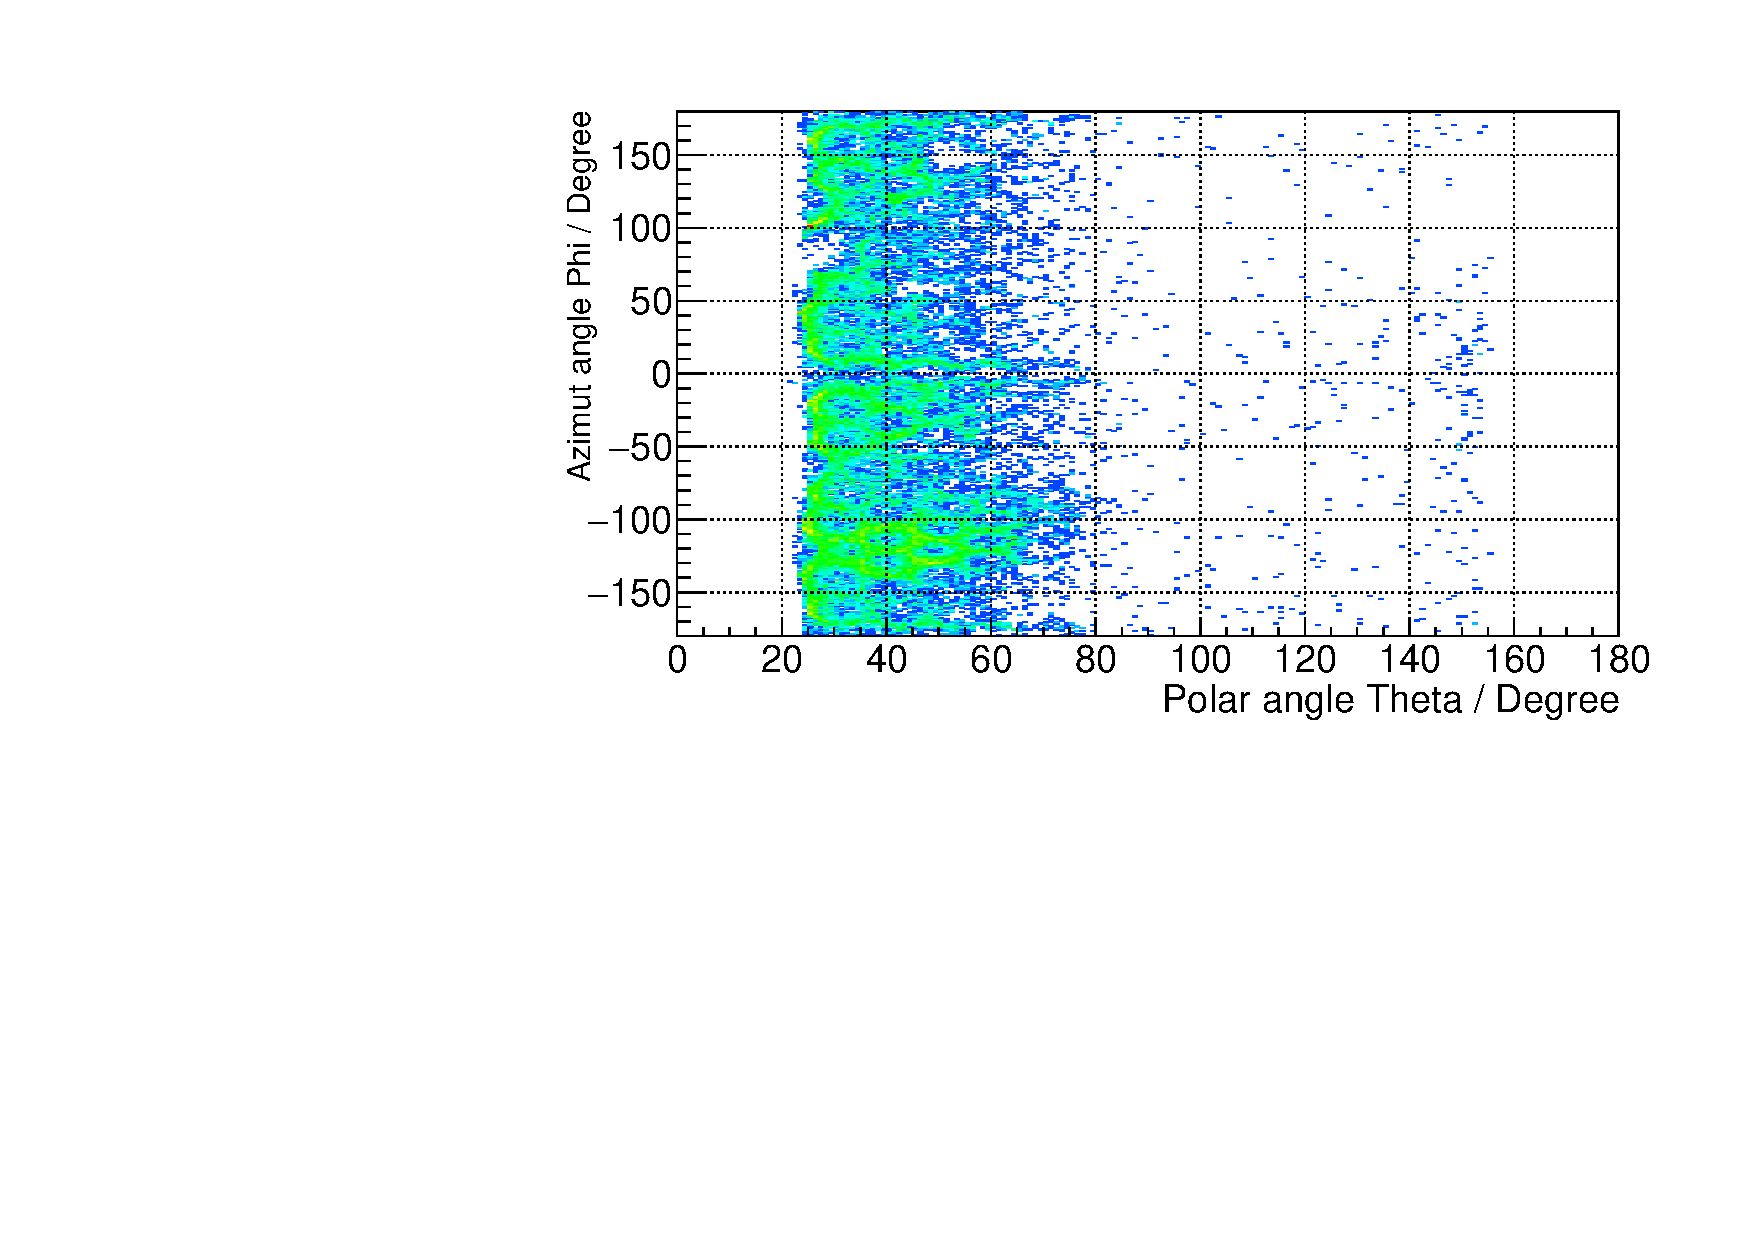
\includegraphics[width=74mm]{20170504ThetaPhiEnergySymmetric2014_10_400}
\end{array}$
\end{center}
	
	\caption[Strahlzeit: Verteilung der symmetrischen Photonen im CB f\"ur verschiedene Energien]{Daten aus der Strahlzeit: Links ist die Verteilung der Photonen im Crystal-Ball mit einer Energie von $125\,\text{MeV}$ bis $150\,\text{MeV}$ zu sehen, rechts von $425\,\text{MeV}$ bis $450\,\text{MeV}$. Es werden nur Photonen mit einer \"ahnlichen Energie ber\"ucksichtigt. Die errechnete invariante Masse muss zwischen $70\,\text{MeV}$ und $200\,\text{MeV}$ liegen.}
	\label{fig:Verteilung-im-CB}
\end{figure}

In den Plots in Abbildung \ref{fig:Verteilung-im-CB} erkennt man sehr gut, wie sich die Verteilung der Photonen \"andert, wenn die Energie der Photonen zunimmt und die Bedingung gilt, dass sich die Energie der Photonen \"ahneln m\"ussen. So sind die Photonen f\"ur kleine Energien \"uber den ganzen Crystal-Ball verteilt, w\"ahrend f\"ur gr\"o{\ss}ere Energien die Photonen immer h\"aufiger am Strahlenausgang auftreten. In dieser Abbildung gibt es einen Schnitt auf die Masse des $\pi^0$. Das bedeutet, die beiden detektierten Photonen werden nur in das Histogramm eingetragen, wenn die aus diesen berechnete invariante Masse zwischen $70\,\text{MeV}$ und $200\,\text{MeV}$ liegt.

Aus der Verbesserung der Abweichung f\"ur hohe Photonenenergien und unter Vernachl\"assigung der Detektoren am Rand liegt die Vermutung nahe, dass die Detektoren am Rand des Strahleneingangs nicht sehr gut f\"ur hohe Photonenenergien kalibriert sind. 
Allerdings ist damit nicht die gesamte Abweichung zu erkl\"aren. 
Aussagen \"uber die Detektoren am Strahleneingang k\"onnen ebenfalls nicht getroffen werden, da diese, im Vergleich zum Strahleneingang, nur sehr selten getroffen werden.

Also muss weiter nach der Ursache f\"ur diese starke Abweichung gesucht werden.



\section{Simulation}
\label{sec:Simulation}

Da mit reellen Daten keine Ursache gefunden werden kann, wodurch diese gro{\ss}e Abweichung entsteht, wird auf simulierte Daten zur\"uckgegriffen. 

Der Grund daf\"ur ist, dass alle Prozesse in simulierten Daten genau bekannt sind. Das hei{\ss}t, von jedem registriertem Teilchen ist bekannt, um welches Teilchen es sich handelt und aus welchem Prozess es entstanden ist. Auch ist die genaue Energie und Trajektorie bekannt.

So kann jeder einzelne Aspekt des Zerfalls genauer untersucht werden.

Als erstes muss \"uberpr\"uft werden, ob die in Kapitel \ref{sec:Energie-Interval-Abhaengigkeit} und \ref{sec:Vernachlaessigung-der-Detektoren-am-Rand} gefundene Abh\"angigkeit auch in der Simulation auftritt. 
Dazu werden zwei Histogramme mit den Bedingungen aus den jeweiligen Kapiteln gef\"ullt. Eins mit den Detektoren am Rand (Abb. \ref{fig:Simulierte-Daten-Abweichung} links) und eins ohne (Abb. \ref{fig:Sim-Data-2DHist-30-Degree-Edge}).

%Anschlie{\ss}end wird \"uber diese dann auch wieder mit der Crystal-Ball-Funktion gefittet, um die $\pi^0$ Position zu bestimmen. Da es sich hier um simulierte Daten handelt, und es keinen st\"orenden Untergrund gibt, ist es nicht n\"otig das Intervall \"uber das gefittet wird, mit der Photonenenergie zu \"andern. Das Intervall wird nun mit 50 MeV bis 220 MeV festgehalten. In Abbildung \ref{fig:Sim-Beispielfit} ist ein Beispielfit f\"ur die simulierten Daten zu sehen. 
%Auch hier werden die beiden Abweichungen vom $\pi^0$-Peak zum besseren Vergleich in einen einzelnen Graphen gezeichnet.

\begin{figure}[h!]
\begin{center}
	$\begin{array}{cc}

	
		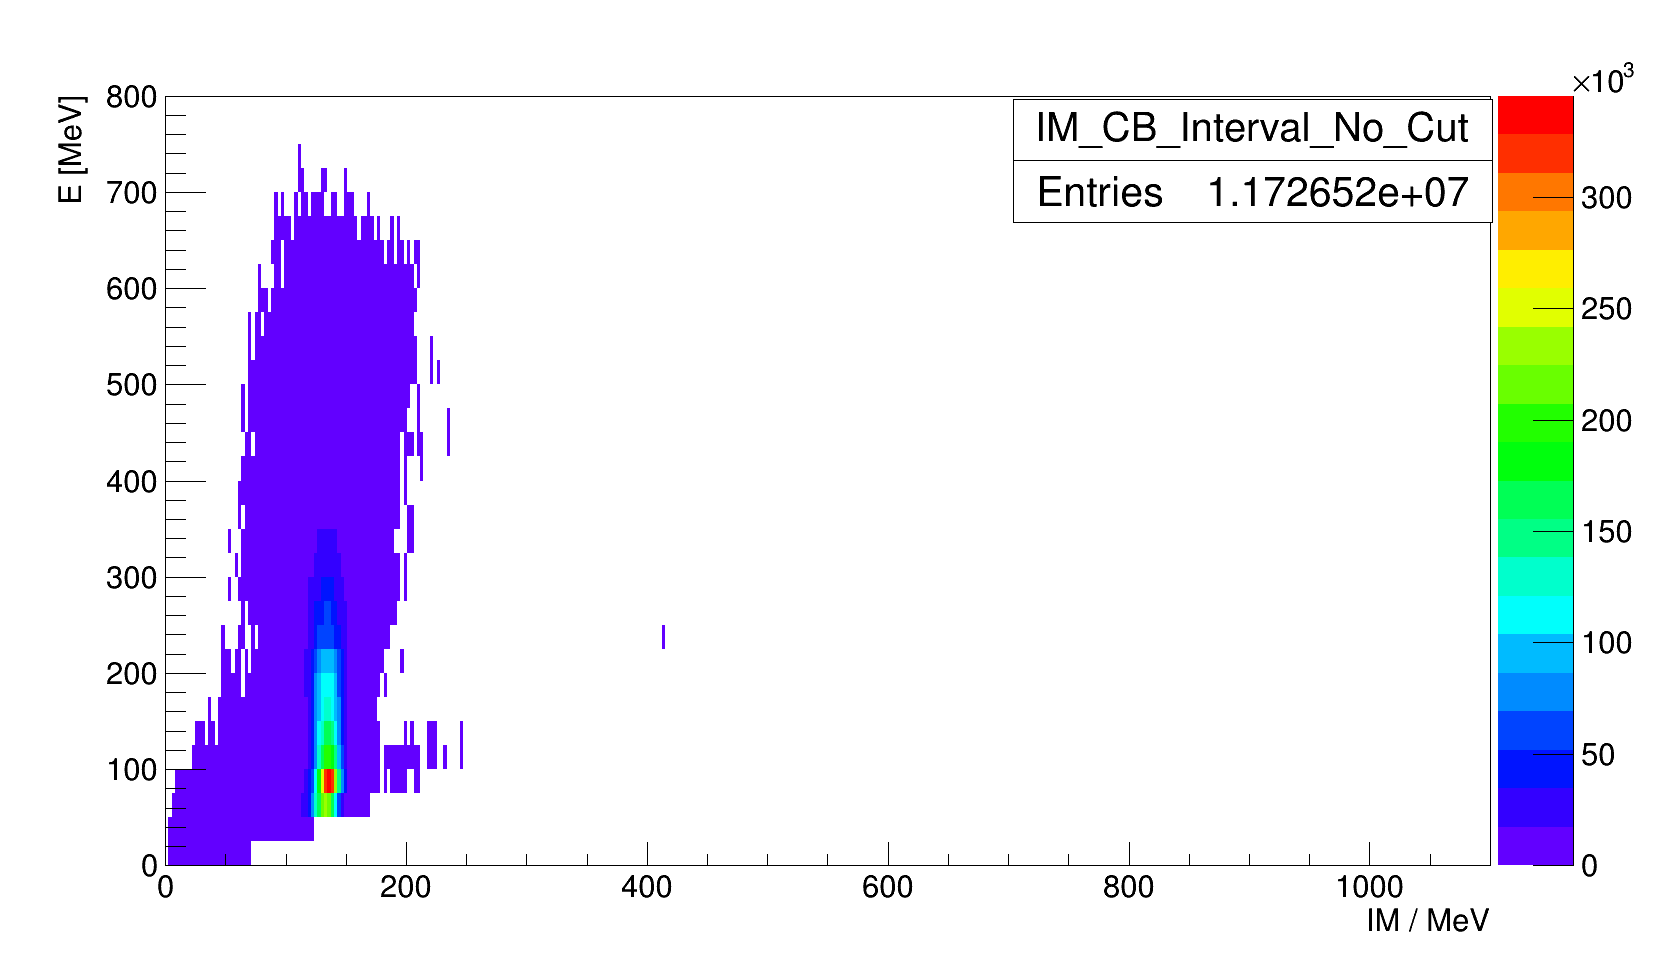
\includegraphics[width=74mm]{NewCalib/20171904SimNoCut2DHist}
	
		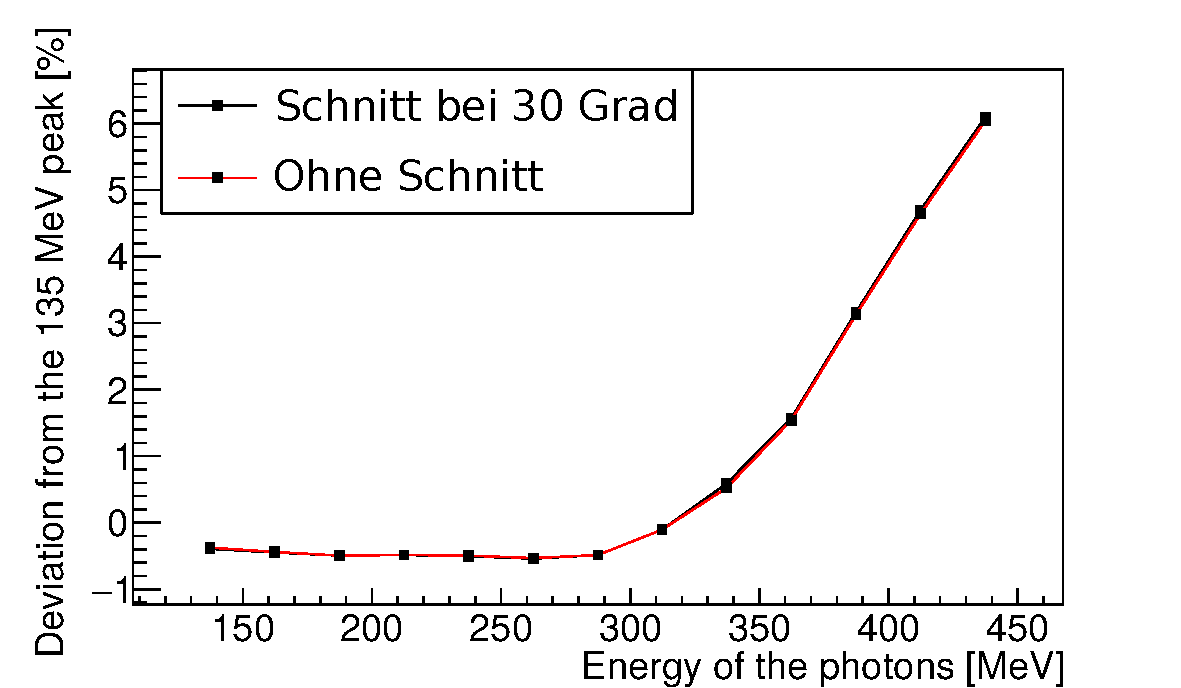
\includegraphics[width=74mm]{20172804MCBothDeviation}
\end{array}$
\end{center}	
	\caption[Simulation: 2D-Histogramm und Abweichung f\"ur symmmetrische Photonen]{Daten aus der Simulation: Links ist als Beispiel das Histogramm aus den simulierten Daten dargestellt. Für dieses Histogramm gilt die Bedingung, dass auch die Detektoren am Rand berücksichtigt werden. Rechts sind die Abweichungen vom $\pi^0$-Peak mit (rot) und ohne (schwarz) Berücksichtigung der Detektoren am Rand zu sehen.}
	\label{fig:Simulierte-Daten-Abweichung}
\end{figure}
%An den beiden Histogrammen erkennt man, dass es sich bei den verwendeten Daten um Simulierte gehandelt hat, da der $\eta$-Peak nicht vorhanden ist. Man hat nur noch einen Peak bei $\pi^0$. 



%Da bei einer Simulation alle Prozesse genau bekannt waren, wurde alles so eingestellt, dass aus dem Cocktail nur $\pi^0 \rightarrow \gamma \gamma\ $ Prozesse betrachtet wurden.

Schon am zweidimensionalem Histogramm aus Abbildung \ref{fig:Simulierte-Daten-Abweichung} ist zu erkennen, dass es sich um simulierte Daten handelte. Es liegt nur ein Peak bei der Masse von $\pi^0$ vor. Einen $\eta$-Peak und einen störenden Untergrund gibt es nicht. 
Deswegen wird zur Bestimmung der $\pi^0$-Position f\"ur die simulierten Daten der Untergrundfit ausgeschaltet, sodass die Crystal-Ball-Funktion die einzige Fitfunktion ist. Der Bereich über den gefittet wird, wird hier mit $50\,\text{MeV}$ bis $220\,\text{MeV}$ konstant gehalten. 

\begin{figure}[h!]
	\begin{center}
		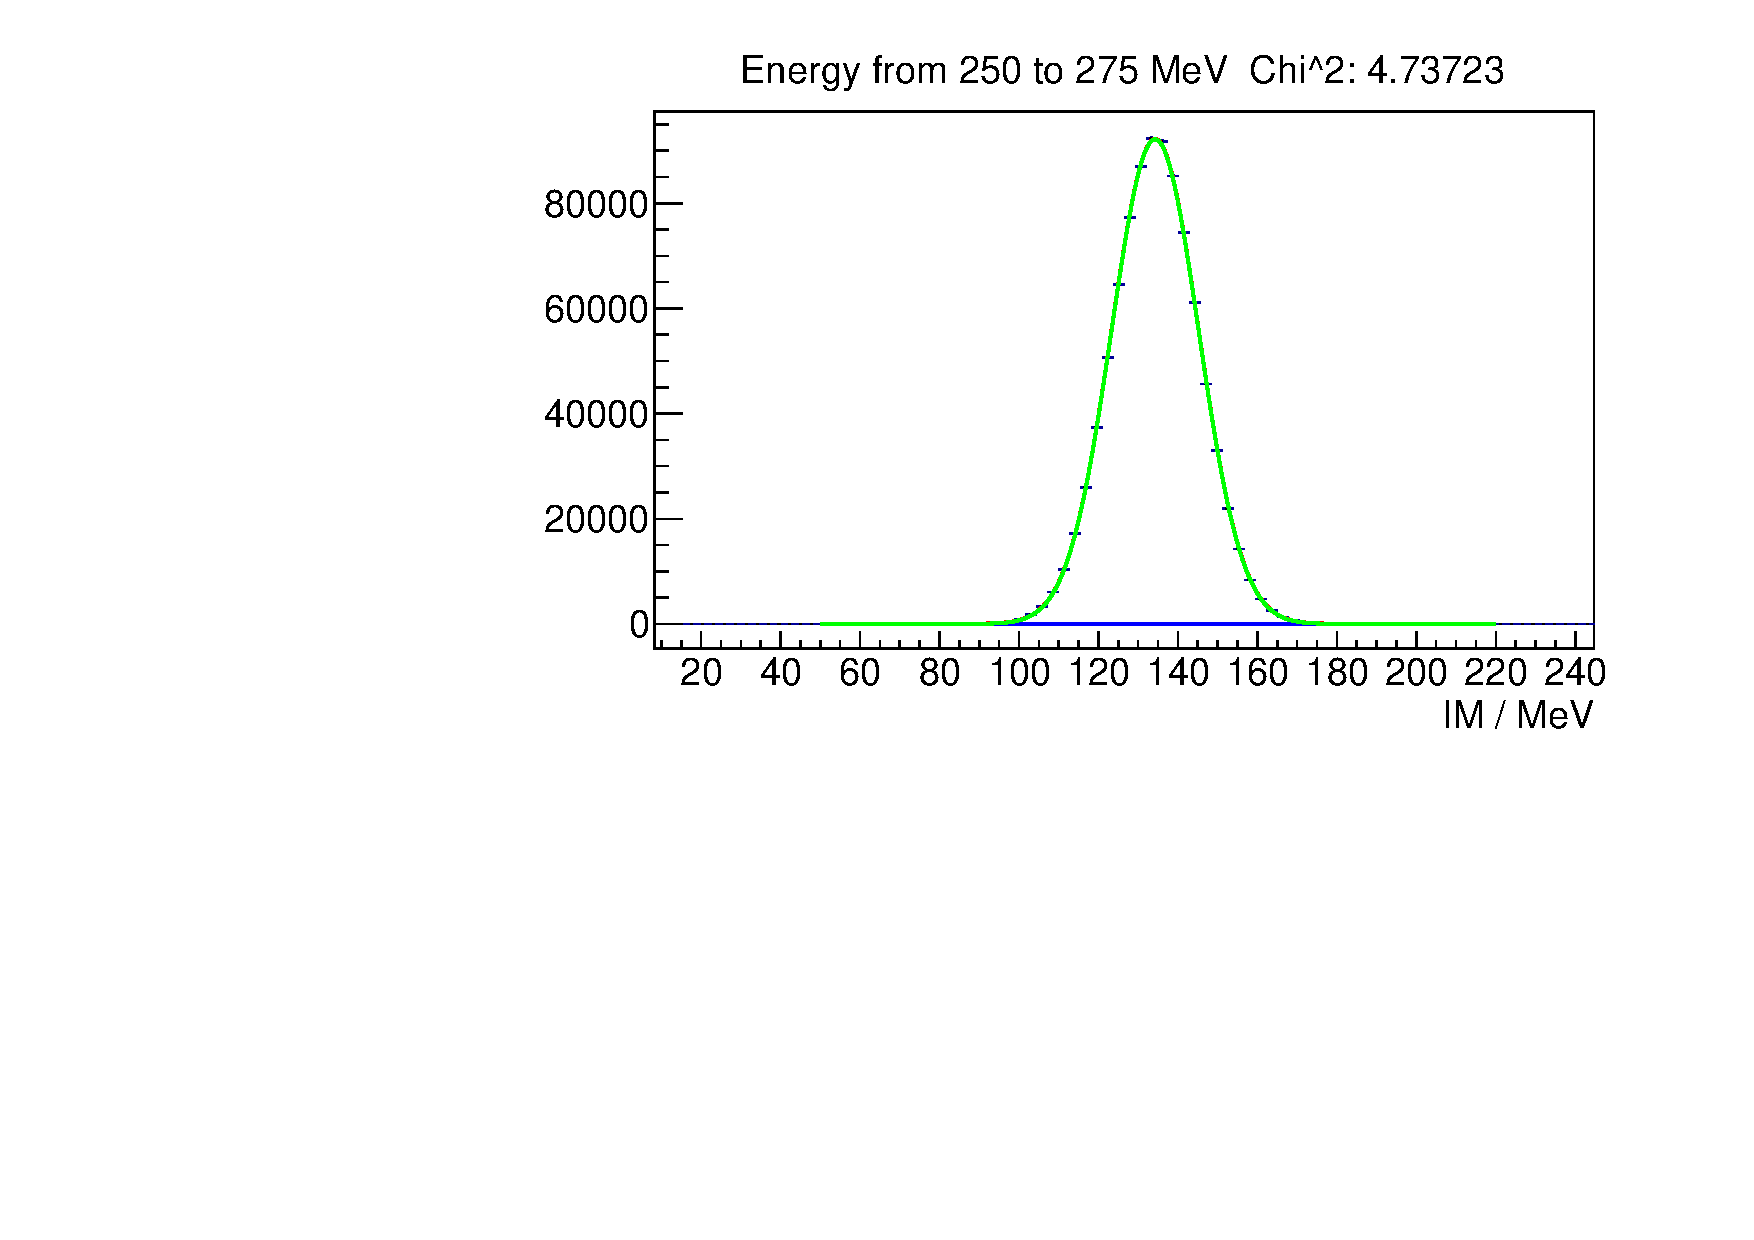
\includegraphics[width=100mm]{20170405SimulierteDatenBeispielFit}
		\caption[Simulation: Beispielfit]{Daten aus der Simulation: Beispielfit}
		\label{fig:Sim-Beispielfit}
	\end{center}
\end{figure}


In Abbildung \ref{fig:Sim-Beispielfit} ist ein Beispielfit f\"ur die simulierten Daten zu sehen, da alle anderen Fits funktioniert haben und sie somit wenig aufschlussreich sind, sollen sie nicht auch noch gezeigt werden. Lediglich Fits mit auffallend gro{\ss}en Fehlerbalken sollen noch aufgef\"uhrt werden. 

Auch hier werden die beiden Abweichungen vom $\pi^0$-Peak zum besseren Vergleich in einen einzelnen Graphen gezeichnet. Dies ist in Abbildung \ref{fig:Simulierte-Daten-Abweichung} rechts zu sehen.

Ebenfalls ist die bei den reellen Daten gefundene Abweichung auch hier für große Photonenenergien zu erkennen. Allerdings ist die Form etwas anders. So ist die Abweichung f\"ur kleine Photonenenergien sehr klein und weniger als -1\% und nimmt auch f\"ur Energien bis $300\,\text{MeV}$ nicht zu, sondern bleibt fast konstant. F\"ur Energien oberhalb von $300\,\text{MeV}$ nimmt die Abweichung mit \"uber +2\% pro $50\,\text{MeV}$ zu. So wird die maximale Abweichung bei einer Photonenenergie von $450\,\text{MeV}$ erreicht. Hier betr\"agt sie ca. 6\%. 

Auch ergibt sich kein Unterschied in den Abweichung für simulierte Daten, wenn die Detektoren am Rand vernachlässigt werden. So muss dieser Grund dafür auch bestimmt werden. Folglich wird damit die Vermutung widerlegt, dass die Detektoren am Rand schlecht eingestellt sind.


%Allerdings war hier der Anstieg der Abweichung im Energieintervall von 200 MeV bis 300 MeV Photonenenergie nur so gering bis nicht vorhanden. Dafür flachte die Abweichung bei den reellen Daten ab einer Photonenenergie von ungefähr 375 MeV ab, während sie bei den simulierten Daten weiter \textit{linear} mit einer \textit{Steigung} von ca. 3\% - 4\% pro 50 MeV Photonenenergie anstieg. Die maximale Abweichung wurde bei einer Energie von 450 MeV erreicht und betrug fast 9\%. Damit war die Abweichung der errechneten Masse aus simulierten Daten größer, als aus reell gemessenen. Auch ergab sich kein Unterschied in den Abweichung für simulierte Daten, wenn die Detektoren am Rand vernachlässigt wurden. So musste dieser Grund dafür auch bestimmt werden. Folglich wurde damit die Vermutung widerlegt, dass die Detektoren am Rand schlecht eingestellt wurden.

Da nun aber trotzdem die Form der Abweichung bei den simulierten Daten ungefähr der Form der reellen Daten für hohe Photonenenergien entspricht, kann die Simulation benutzt werden, um ihre Ursache zu bestimmen.

%Ein weiterer Vorteil einer Simulation war, dass man von jedem detektierem Teilchen wusste, woher es kam und worum es sich dabei handelte. Folglich konnte alles so eingestellt werden, dass aus dem Cocktail nur $\pi^0 \rightarrow \gamma \gamma$ Prozesse betrachtet wurden.

\subsection{Mindestwinkel zwischen detektierten Photonen}
\label{sec:Min-Openingangle}

%\colorbox{yellow}{\"Offnungswinkel ist mindestens 30 Grad; Mit Detektoren Am Rand}
Als erstes wird \"uberpr\"uft, ob sich eine Verkleinerung der Abweichung ergibt, wenn man die Bedingung stellt, dass zwischen den beiden detektierten Photonen ein Mindestwinkel vorliegen muss. 
Wie bereits erw\"ahnt, breitet sich ein Schauer im Detektor immer auch in transversaler Richtung aus. Also werden mehrere Detektoren durch ein einfallendes Photon ausgel\"ost. 
Es m\"ussen die bereits in Abschnitt \ref{sec:Clustering-Algorithmus} gestellten Bedingungen erf\"ullt sein, damit ein Detektor als ausgel\"ost eingestuft wird.

Es ist allerdings auch m\"oglich, dass ein Detektorkristall von zwei Photonen ausgel\"ost werden kann, wenn der \"Offnungswinkel zwischen den beiden Photonen nicht gro{\ss} genug ist, um eine \"Uberlagerung zu vermeiden. Das f\"uhrt dazu, dass die Energie und der Auftreffort der Photonen nicht exakt rekonstruiert werden kann, da die Aufteilung der berechneten Energie auf die beiden Photonen nicht eindeutig festgelegt werden kann.

Deswegen wird hier darauf geachtet, dass die registrierten Photonen einen \"Offnungswinkel von mindestens 30$^{\circ}$ besitzen, um eine solche \"Uberlagerung zu vermeiden.
Die Energie der Photonen muss sich auch wieder \"ahneln.
Die Detektoren am Rand werden hier auch ber\"ucksichtigt, da sich dadurch keine Verbesserung in Kapitel \ref{sec:Simulation} ergab.

Es wird also auch wieder ein zweidimensionales Histogramm angelegt (Abb. \ref{fig;2D-Hist-Min-OpeningAngle}), \"uber das gefittet wird. Bereits an dem zweidimensionalem Histogramm erkennt man, dass nur sehr wenige bis gar keine hochenergetischen Photonen vorliegen.

\begin{figure}[h!]
	\begin{center}
		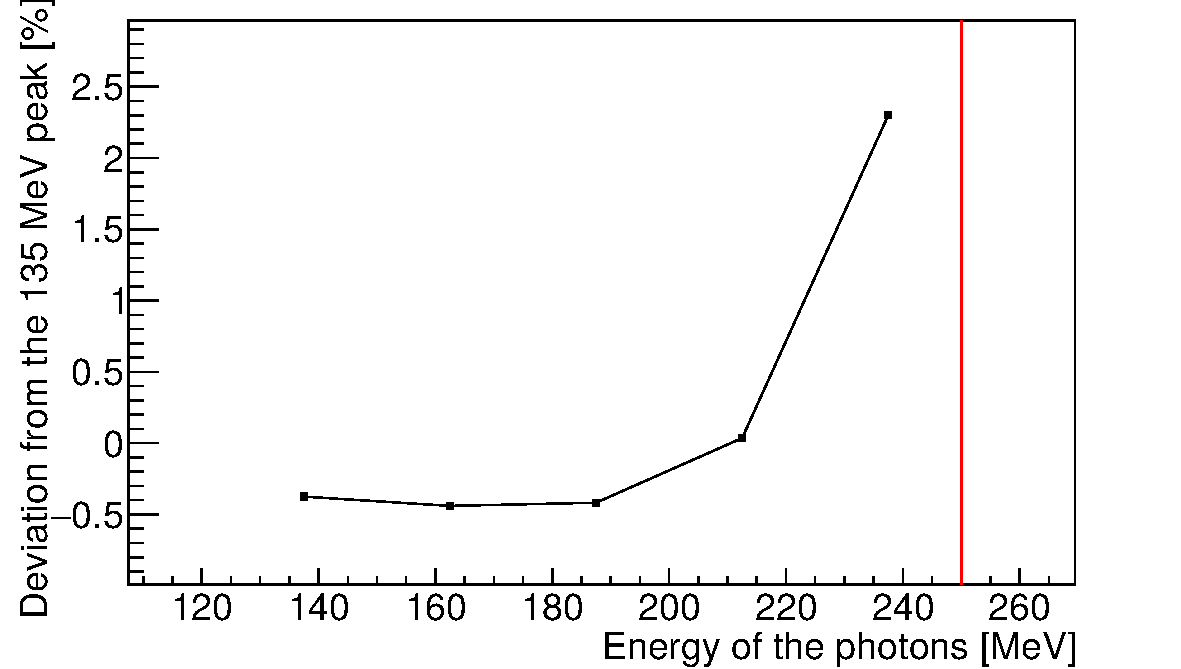
\includegraphics[width=100mm]{20170505MinAngle30Deviation}
		\caption[Simulation: Abweichung für Mindestwinkel zwischen detektierten Photonen]{Daten aus der Simulation: Die Abweichung der $\pi^0$-Peak Position mit der Bedingung, dass der \"Offnungswinkel zwischen den beiden detektierten Teilchen mindestens 30$^{\circ}$ betr\"agt. Die rote Linie markiert die Photonenenergie, ab der keine Photonenpaare mit einem Winkel von \"uber 30$^{\circ}$ gefunden werden k\"onnen.}
		\label{fig:Relative-Abweichung-Min-Opening-Angle}
	\end{center}
\end{figure}

Wie in Abbildung \ref{fig:Relative-Abweichung-Min-Opening-Angle} zu erkennen ist, \"ahnelt f\"ur kleine Photonenenergien die hier bestimme Abweichung sehr stark der bereits gefundenen in Kapitel \ref{sec:Simulation}.

Auch hier ist die Abweichung zun\"achst sehr klein und liegt etwas im negativen. Es liegt fast keine \"Anderung der Abweichung vor. Dies gilt bis zu einer Photonenenergie von $200\,\text{MeV}$.
Ab einer Photonenenergie von \"uber $200\,\text{MeV}$ nimmt die Abweichung allerdings zu. Sodass hier schon bei einer Photonenenergie von $250\,\text{MeV}$ eine Abweichung von \"uber 2\% vorliegt. 
Auffallend ist, dass die Abweichung hier schon im Gegensatz zu Abbildung \ref{fig:Simulierte-Daten-Abweichung} rechts schon fr\"uher anf\"angt zu steigen. Dort fing es erst ab einer Photonenenergie von $300\,\text{MeV}$ an zu steigen.

In der Abbildung ist auch die Grenze markiert, ab der keine Photonenpaare mit einem \"Offnungswinkel von \"uber 30$^{\circ}$ detektiert werden.
Dieses Ph\"anomen wird nun genauer untersucht.

Dazu wird als erstes bestimmt, welchen \"Offnungswinkel $\alpha$ man f\"ur verschiedene Photonenenergien erh\"alt, wenn die Bedingung gilt, dass die Energie der Photonen \"ahnlich sein muss.
Dazu werden die Daten aus dem Ereignisgenerator entnommen.


\begin{figure}[h!]
	\begin{center}
		$\begin{array}{cc}
		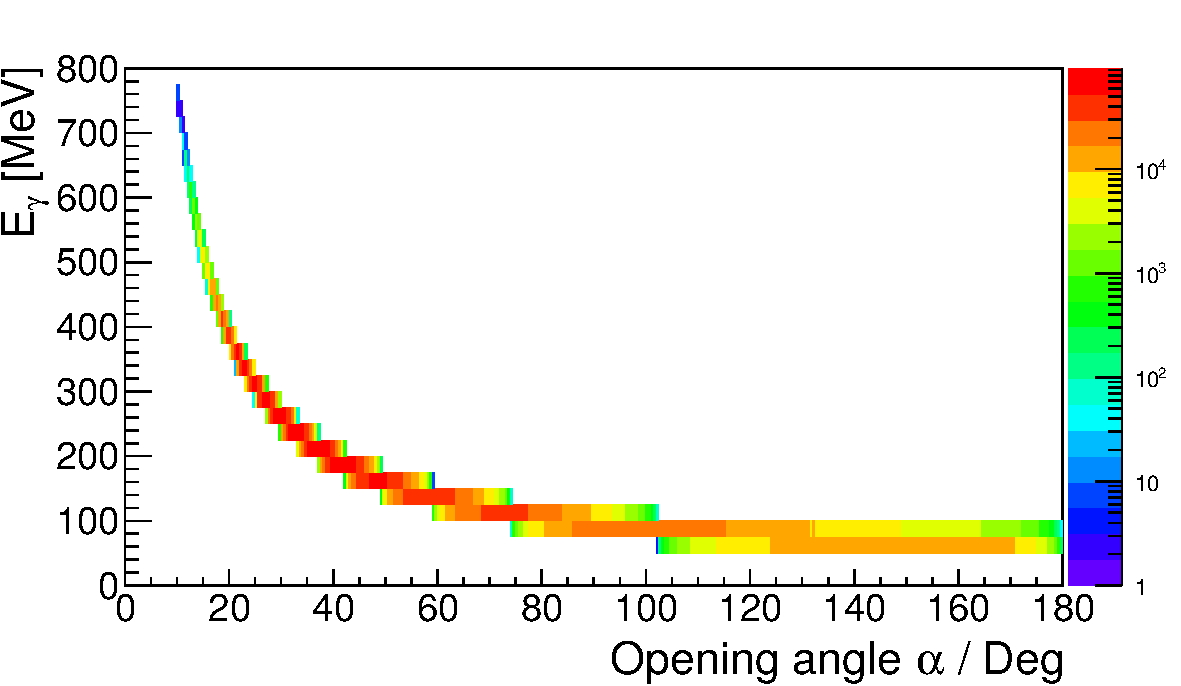
\includegraphics[width=80mm]{20172804TrueOpeningAngle}
		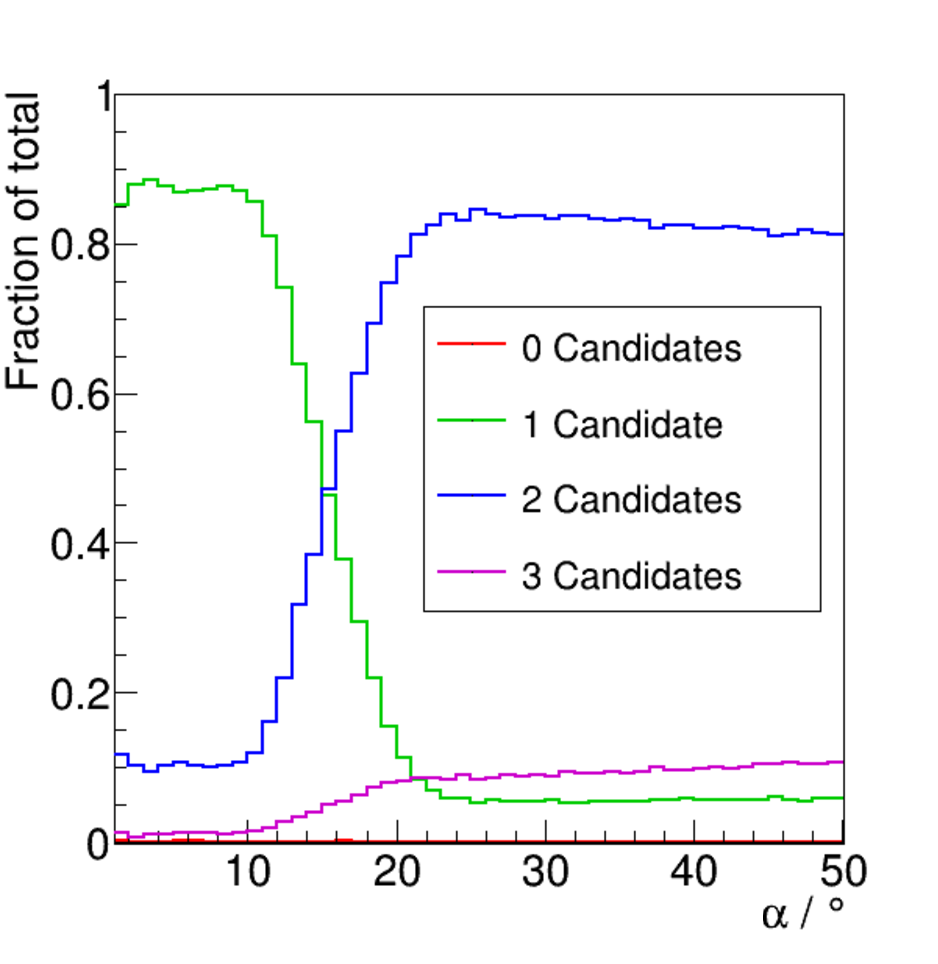
\includegraphics[width=70mm]{MCClusteringCheck_nCandsOpAng}
		\end{array}$
		\caption[Ereignisgenerator: \"Offnungswinkel vs. Photonenenergie; Clusteralgorithmus f\"ur verschiedene \"Offnungswinkel]{Links: Daten aus dem Ereignisgenerator: \"Offnungswinkel $\alpha$ f\"ur verschiedene Photonenenergien; Rechts: Anzahl der gemessenen Kandidaten gegen verschiedene \"Offnungswinkel. Die Photonenenergie liegt dabei in einem Intervall von $0\,\text{MeV}$ bis $1600\,\text{MeV}$ ohne die Bedingung, dass die Photonen eine ähnliche Energie besitzen müssen. Rechter Plot:\cite{Ne17}}
		\label{fig:True-OpeningAngle}
	\end{center}
\end{figure}

In Abbildung \ref{fig:True-OpeningAngle} links ist zu sehen, wie der \"Offnungswinkel $\alpha$ f\"ur gr\"o{\ss}er werdende Energien kleiner wird. Aus der Abbildung kann man auch entnehmen, dass f\"ur einen \"Offnungswinkel von 30$^{\circ}$ die maximale Photonenenergie $250\,\text{MeV}$ betr\"agt.

Jetzt liegt die Vermutung nat\"urlich nahe, dass die durch die Photonen ausgel\"osten Cluster sich \"uberlagern. 

In der gleichen Abbildung rechts erkennt man, dass f\"ur \"Offnungswinkel unter 20$^{\circ}$ der Cluster-Algorithmus anf\"angt, aus mehreren Kandidaten, also Teilchen die im Crystal-Ball detektiert werden, einen zu machen.

Unterhalb von einem \"Offnungswinkel von ca. 15$^{\circ}$ werden schlie{\ss}lich zwei Events in Crystal-Ball h\"aufiger durch den Cluster-Algorithmus zu einem zusammengefasst als getrennt. 

Wenn die zwei Cluster sich \"uberlagern und durch den Algorithmus zusammengefasst werden, dann l\"asst sich der \"Offungswinkel zwischen den beiden Teilchen nicht eindeutig bestimmen.

Da hier allerdings ein \"Offnungswinkel von mindestens 30$^{\circ}$ gefordert wird, kommt der Algorithmus zur Clusterbildung nicht in Frage.
Es kann nur sein, dass der $\pi^0$-Peak ab einer Photonenenergie von $225\,\text{MeV}$ zu stark durch den Untergrung gest\"ort wird, da dieser durch diesen Schnitt nicht reduziert wird, die St\"arke des $\pi^0$-Peaks allerdings schon.
%Folglich ergibt die Bedingung, dass der \"Offnungswinkel zwischen den beiden detektierten Photonen mindestens 30$^{\circ}$ sein muss, keine Verbesserung und es muss weiter nach einer Ursache f\"ur die Abweichung gesucht werden.




\subsection{Isotroper Zerfall von $\pi^0$ im Ursprung}
\label{sec:Isotroper-Zerfall-Ursprung}

Als n\"achstes wird der einfachste Prozess \"uberpr\"uft. Dazu zerf\"allt ein $\pi^0$ im Ursprung und erh\"alt einen Boost in eine zufällige Richtung. Dadurch gibt es keine ausgezeichnete Richtung. Folglich kann damit überprüft werden, ob sich alle Detektoren gleich verhalten. 

Dazu wird der neue Ereignisgenerator so eingestellt, dass es keinen Photonenstrahl und kein Proton mehr gibt, lediglich der Boost des $\pi^0$ wird gewürfelt. Die Photonen werden dann anschließend, wie in Kapitel \ref{sec:Vorbereitung-der-Simulation} beschrieben, gewürfelt und geboostet. 
Als erste Kontrolle wird \"uberpr\"uft, ob die durch den Zerfall ausgesandten Photonen sich auch wirklich gleichm\"a{\ss}ig im Raum verteilen.


\begin{figure}[h!]
\begin{center}
	$\begin{array}{cc}

		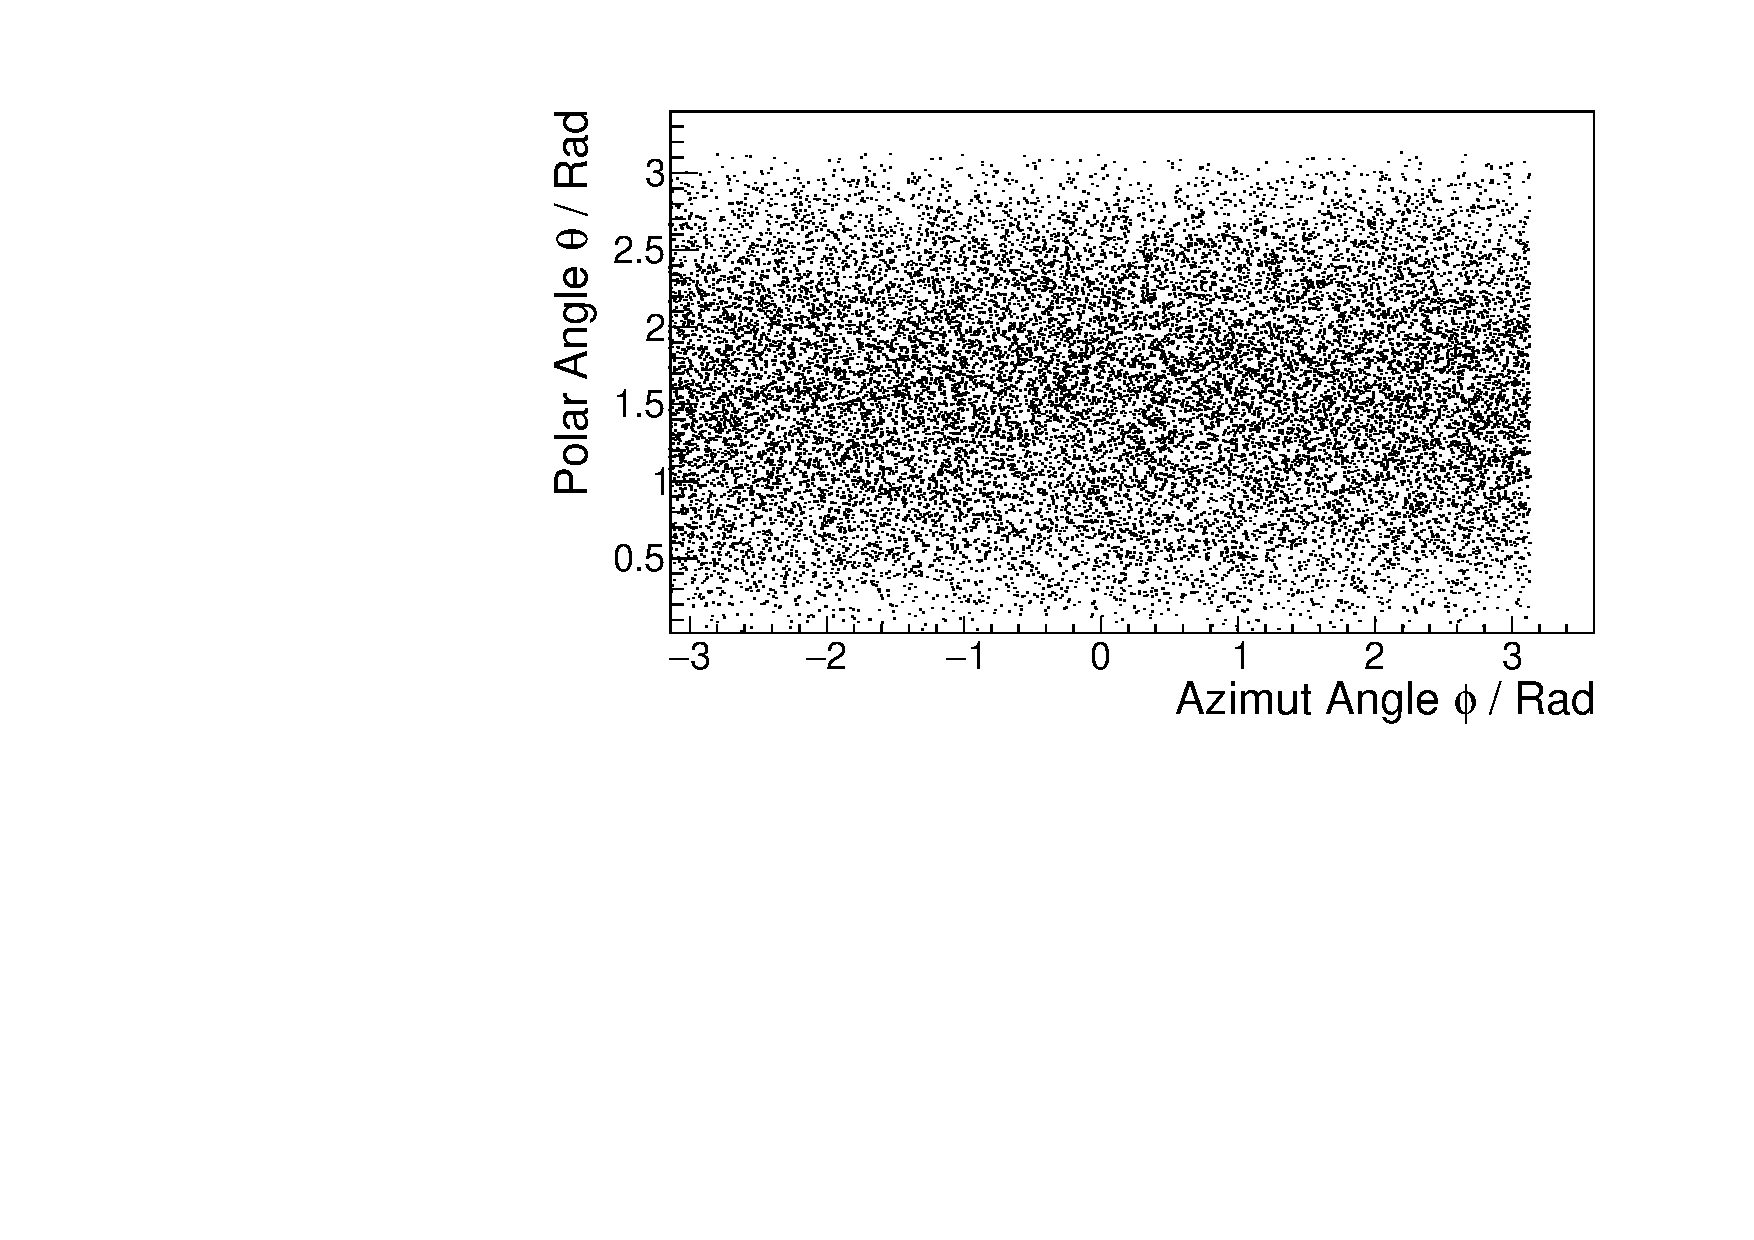
\includegraphics[width=74mm]{20171005Pi0UrsprungThetaPhiVerteilung}

		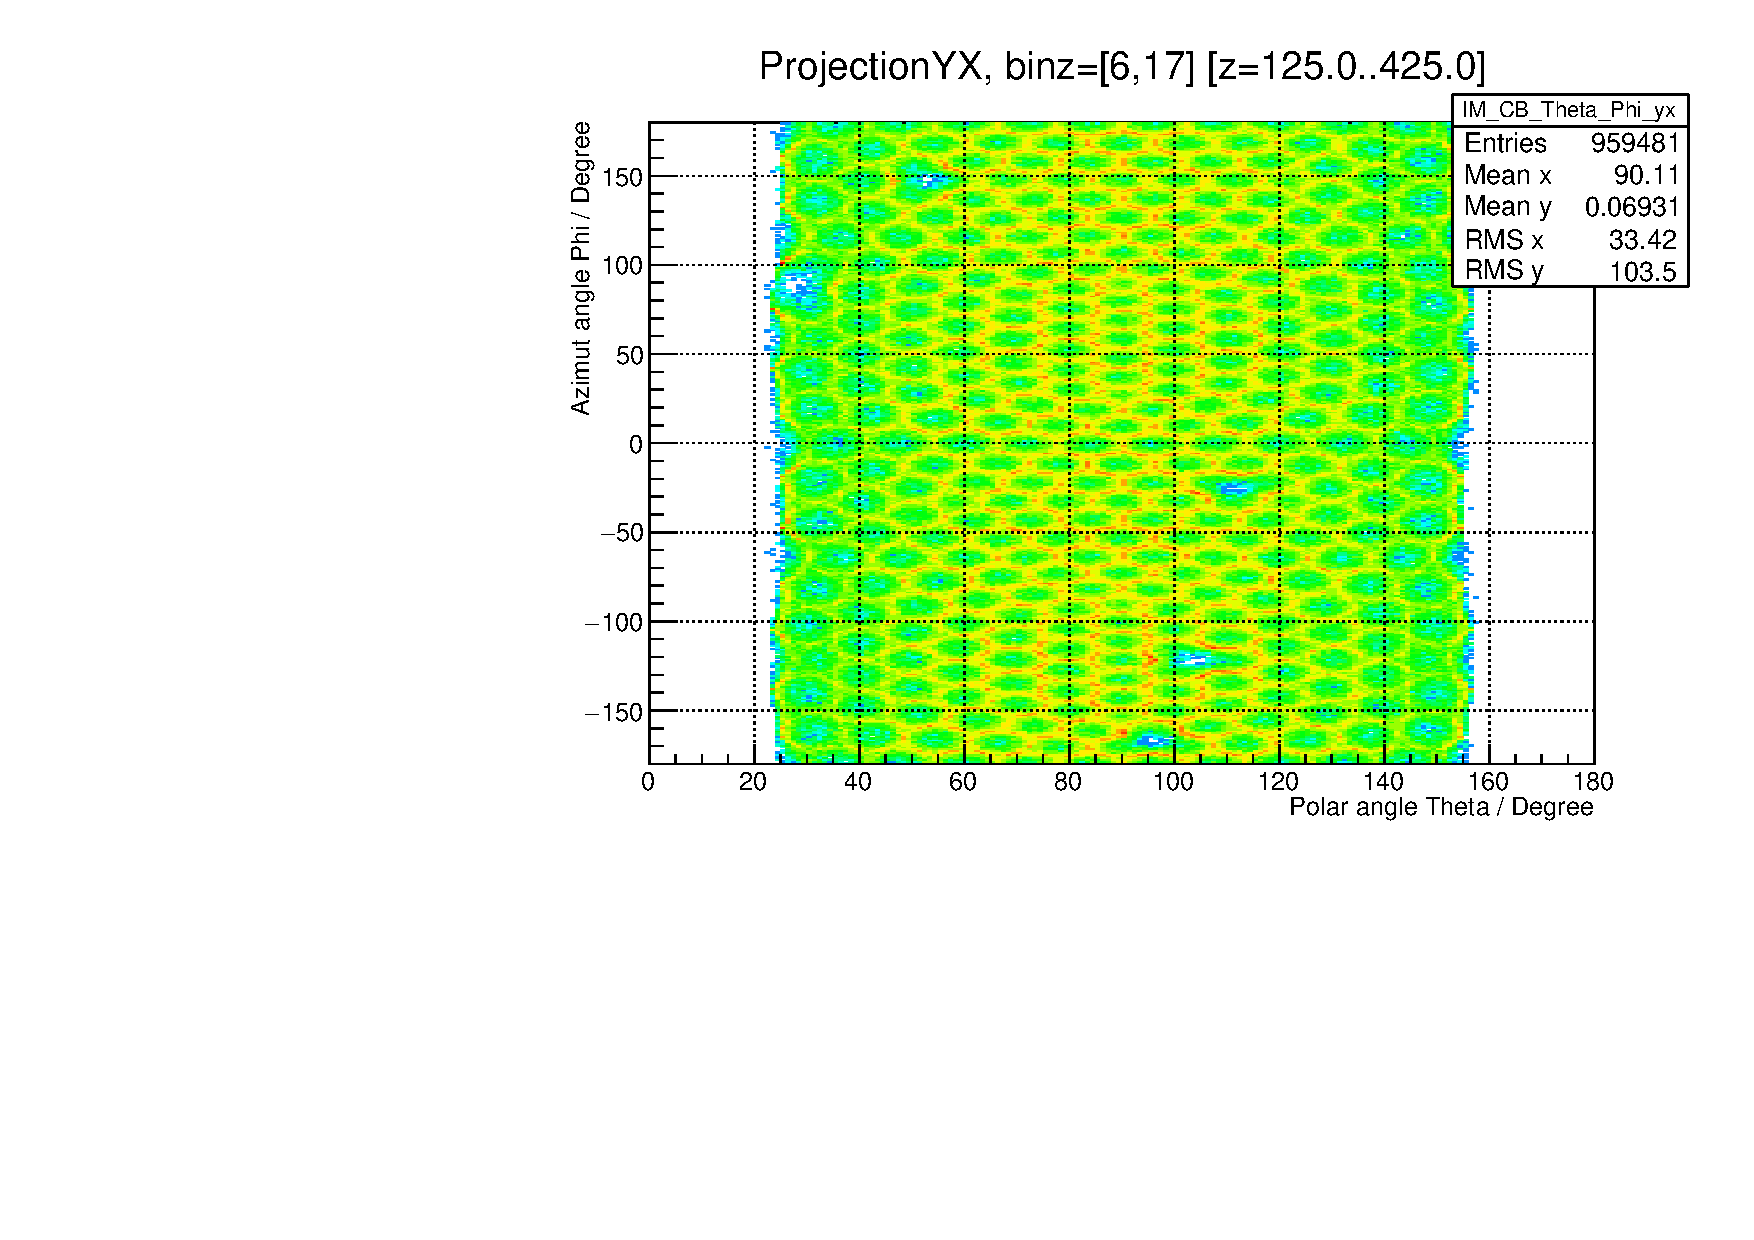
\includegraphics[width=74mm]{20171204DistributionPhotonUrsprungIsotrop}
\end{array}$
\end{center}
\caption[Simulation: Verteilung der Mesonen und detektierten Photonen im CB bei isotropen Zerfall] {Daten aus der Simulation: Ursprung: Isotroper Boost: Links ist die Verteilung der geboosteten $\pi^0$ im Raum zu erkennen. Rechts ist der Ort dargestellt, an dem die Photonen den Crystal-Ball treffen. Durch die Bestimmung des Auftreffortes mit dem Clustering-Algorithmus entsteht dieses Netzmuster. Die Photonen m\"ussen sich energetisch \"ahneln. Au{\ss}erdem werden nur Photonen mit einer Energie zwischen $125\,\text{MeV}$ und $450\,\text{MeV}$ ber\"ucksichtigt.}
\label{fig:Verteilung-von-Mesonen-und-Photonen-im-Raum}
\end{figure}

In Abbildung \ref{fig:Verteilung-von-Mesonen-und-Photonen-im-Raum} links erkennt man, dass die $\pi^0$ einen Boost in eine zuf\"allige Raumrichtung erhalten. Dadurch sind die durch den Zerfall ausgesandten Photonen isotrop im Raum verteilt.
Zus\"atzlich gilt die Bedingung, wie in den vorherigen Kapiteln, dass nur Photonen mit einer ähnlichen Energie als Ereignis in die Datei geschrieben werden d\"urfen.

In Geant wird zus\"atzlich die Länge des Target auf $0\,\text{cm}$ gesetzt. Dadurch wird gewährleistet, dass die Pionen auch wirklich im Ursprung zerfallen.


%Au{\ss}erdem ben\"otigte das Simulieren des Crystal-Balls sehr viel Zeit. So dauerte es zum Simulieren von 100000 Prozessen etwa zwei Stunden. Von diesen mussten die meisten verworfen werden, weil Photonen entstanden, deren Energie sich nicht \"ahnelte. Folglich w\"urde man ein Packet mit mehreren Millionen reinen $\pi^0 \rightarrow \gamma \gamma $ Prozessen ben\"otigen, um genug Ereignisse zu erhalten. So wurde ein Paket benutzt, welches 10 Millionen dieser Prozesse beinhaltete, allerdings war es trotzdem nicht gro{\ss} genug, um eine gute Statistik zu erhalten. gr\"o{\ss}ere Pakete existierten nicht.

%Um nun  eine lange Simulaiton zu vermeiden, wurde beim Erstellen der Simulation \"uber Pluto, bereits hier die Energie der beiden Photonen \"uberpr\"uft. Nur dann wurde der Zerfall von Pluto eingetragen und anschlie{\ss}end \"uber GEANT4 simuliert. Dies hatte eine erhebliche Zeitersparnis zur Folge.

Um zu überprüfen, ob alles wie gewollt eingestellt ist, wird ein weiteres zweidimensionales Histogramm angelegt.



In Abbildung \ref{fig:Verteilung-von-Mesonen-und-Photonen-im-Raum} rechts sieht man, dass sich die Pionen gleichm\"a{\ss}ig im Raum verteilen und es keine ausgezeichnete Richtung gibt. Also ist alles wie gew\"unscht eingestellt, wodurch das weitere Verhalten des Crystal-Balls betrachtet werden kann.

Nun wird wie in den vorherigen Kapiteln ein Histogramm mit den Photonen gefüllt (Abb. \ref{fig:Sim-Data-Ursprung-2DHist-No-Cut}) und anschließend wird über die verschiedenen Photonenenergien gefittet. Dies wird sowohl mit, als auch ohne Berücksichtigung der Detektoren am Rand durchgeführt.

\begin{figure}[h!]
	\begin{center}
		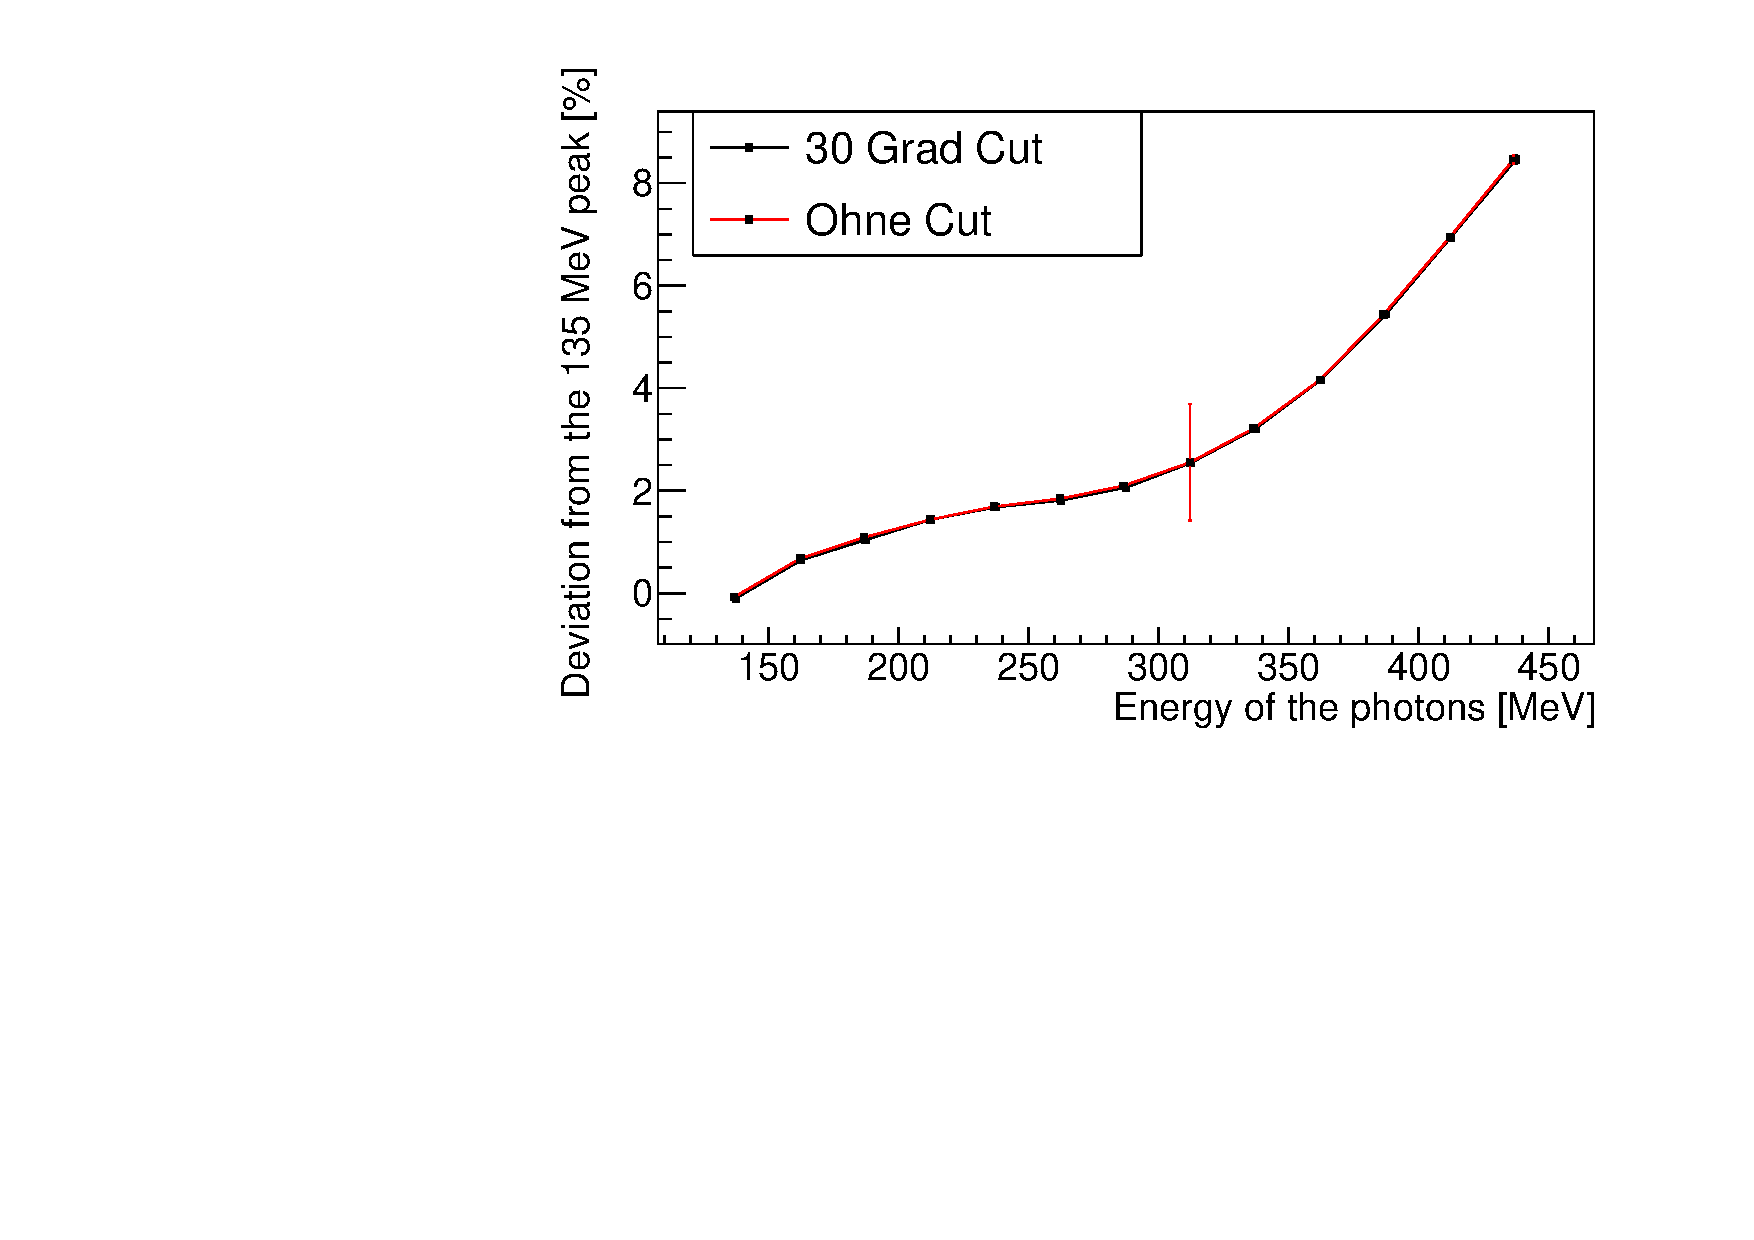
\includegraphics[width=100mm]{20172804IsotropUrpsprungDeviation}
	\end{center}
\caption[Simulation: Isotroper Zerfall Abweichung mit und ohne Detektoren am Rand]{Daten aus der Simulation: Ursprung: Isotroper Boost: Abweichung der errechneten invarianten Masse von der tatsächlichen $\pi^0$ Masse in Prozent. Bei der roten Linie werden die Detektoren am Rand berücksichtigt, bei der schwarzen werden sie vernachlässigt.}
\label{fig:Pi0-Ursprung-Relative-Abweichung}
\end{figure}



In der Abbildung \ref{fig:Pi0-Ursprung-Relative-Abweichung} ist die Abweichung der errechneten invarianten Masse für verschiedene Photonenenergien aufgetragen.
Hier gibt es einen Ausrei{\ss}er. F\"ur eine Photonenenergie von $300\,\text{MeV}$ bis $325\,\text{MeV}$ ohne Cut besitzt eine Abweichung einen sehr gro{\ss}en Fehlerbalken. Allerdings kann man diesen nicht nachvollziehen, wenn man sich den Fit betrachtet. Siehe dazu Abbildung \ref{fig:Isotrop-Fit-Fail}.

 Die Form der Abweichung ähnelt sehr stark der aus Abbildung \ref{fig:Simulierte-Daten-Abweichung}.
 Allerdings gibt es hier kein Plateau im Photonenenergieintervall von $125\,\text{MeV}$ bis $300\,\text{MeV}$, sondern es liegt hier eine sehr leichte \textit{Steigung} von etwa +0,2\% pro $50\,\text{MeV}$ vor. Die maximale Abweichung liegt hier ebenfalls bei $450\,\text{MeV}$ und betr\"agt über +8\%. Auch hier ist kein Unterschied zwischen den Abweichungen zu erkennen, wenn man die Detektoren am Rand berücksichtigt oder vernachlässigt. 

Daraus folgt, dass auf eine andere Weise nach der Ursache für die Abweichung gesucht werden muss, da die starke Vereinfachung des zu untersuchenden Prozesses nicht weiter geholfen hat.

%Nun wurde \"uberpr\"uft, wie sich die Abweichung des $\pi^0$-Peaks verhielt, wenn das $\pi^0$ einen zuf\"alligen Boost in eine beliebige Richtung erhielt. Dazu wurde ein dreidimensionales Histogramm angelegt, mit der errechneten invarianten Masse auf der x-Achse, der Energie der Photonen auf der y-Achse und der Energie des geboosteten Mesons auf der z-Achse. Es galt immer noch die Bedingung, dass die detektierten Photonen eine \"ahnliche Energie aufweisen mussten, um in das Histogramm gef\"ullt zu werden.

\subsection{$z$-Vertex Abh\"angigkeit}
\label{sec:Z-Vertex-Abhaengigkeit}


Zusätzlich wird auch die Abh\"angigkeit, zwischen der errechneten  Position des $\pi^0$-Peaks und dem Ort im Target in dem das Pion entstanden und zerfallen ist, \"uberpr\"uft. 

Da das $\pi^0$ nur wenige Nanometer zur\"ucklegt, bevor es zerf\"allt, kann angenommen werden, dass das Pion am gleichem Ort zerf\"allt, an dem es auch entsteht.

% Hier wurde schlie{\ss}lich ein weiterer Vorteil der Simulation ausgenutzt. Bei einer Simulation sind alle Prozesse genau bekannt. Von jedem Prozess wusste man demnach auch den genauen Ort an dem er sich ereignete. Bei reellen Messdaten war dies nicht m\"oglich, da der Crystal-Ball keinen Detektor besa{\ss}, um den Ort des Zerfalls zu bestimmen. 

Zur Untersuchung der $z$-Vertex Abhängigkeit wird das $ 10\,\text{cm}$ lange Fl\"ussig-Wasserstoff-Target im Zentrum des Crystal-Ball Detektor in zehn $1\,\text{cm}$ lange Intervalle unterteilt. 
Im Zentrum des Targets befindet sich der Ursprung des Koordinatensystems, so liegt am Anfang des Targets das Intervall von $z=-5\,\text{cm}$ bis $z=-4\,\text{cm}$, dann folgt $z=-4\,\text{cm}$ bis $z=-3\,\text{cm}$ usw. 

Hier wird ein weiterer Vorteil der Simulation ausgenutzt. Aus den im Experiment genommenen Daten kann n\"amlich nicht der Ort bestimmt werden, an dem das $\pi^0$ zerfallen ist. Daf\"ur gibt es keine Detektoren im Crystal-Ball. In Simulationen sind alle Prozesse allerdings wohl bekannt, so wei{\ss} man auch von jedem Prozess an welchem Ort er sich ereignet. 

Anschließend wird ein dreidimensionales Histogramm angelegt mit den Intervallen des $z$-Vertex auf der $z$-Achse, der errechneten invarianten Masse auf der $x$-Achse und der Energie der Photonen auf der $y$-Achse angelegt. (Abb.: \ref{fig:Z-Vertex-3D-Hist}). Die Detektoren am Rand werden nicht ber\"ucksichtigt.

Daraus kann dann die Position des $\pi^0$-Peaks in Abhängigkeit zum $z$-Vertex Intervall berechnet werden, dazu wird jedes $z$-Intervall einzeln betrachtet und die Position abhängig von der Energie der Photonen berechnet. 
Diese 10 $z$-Vertex Abhängigkeiten werden anschließend in Abbildung \ref{fig:Z-Vertex-Multi-Graph} eingetragen.

\begin{figure}[h!]
	\begin{center}
		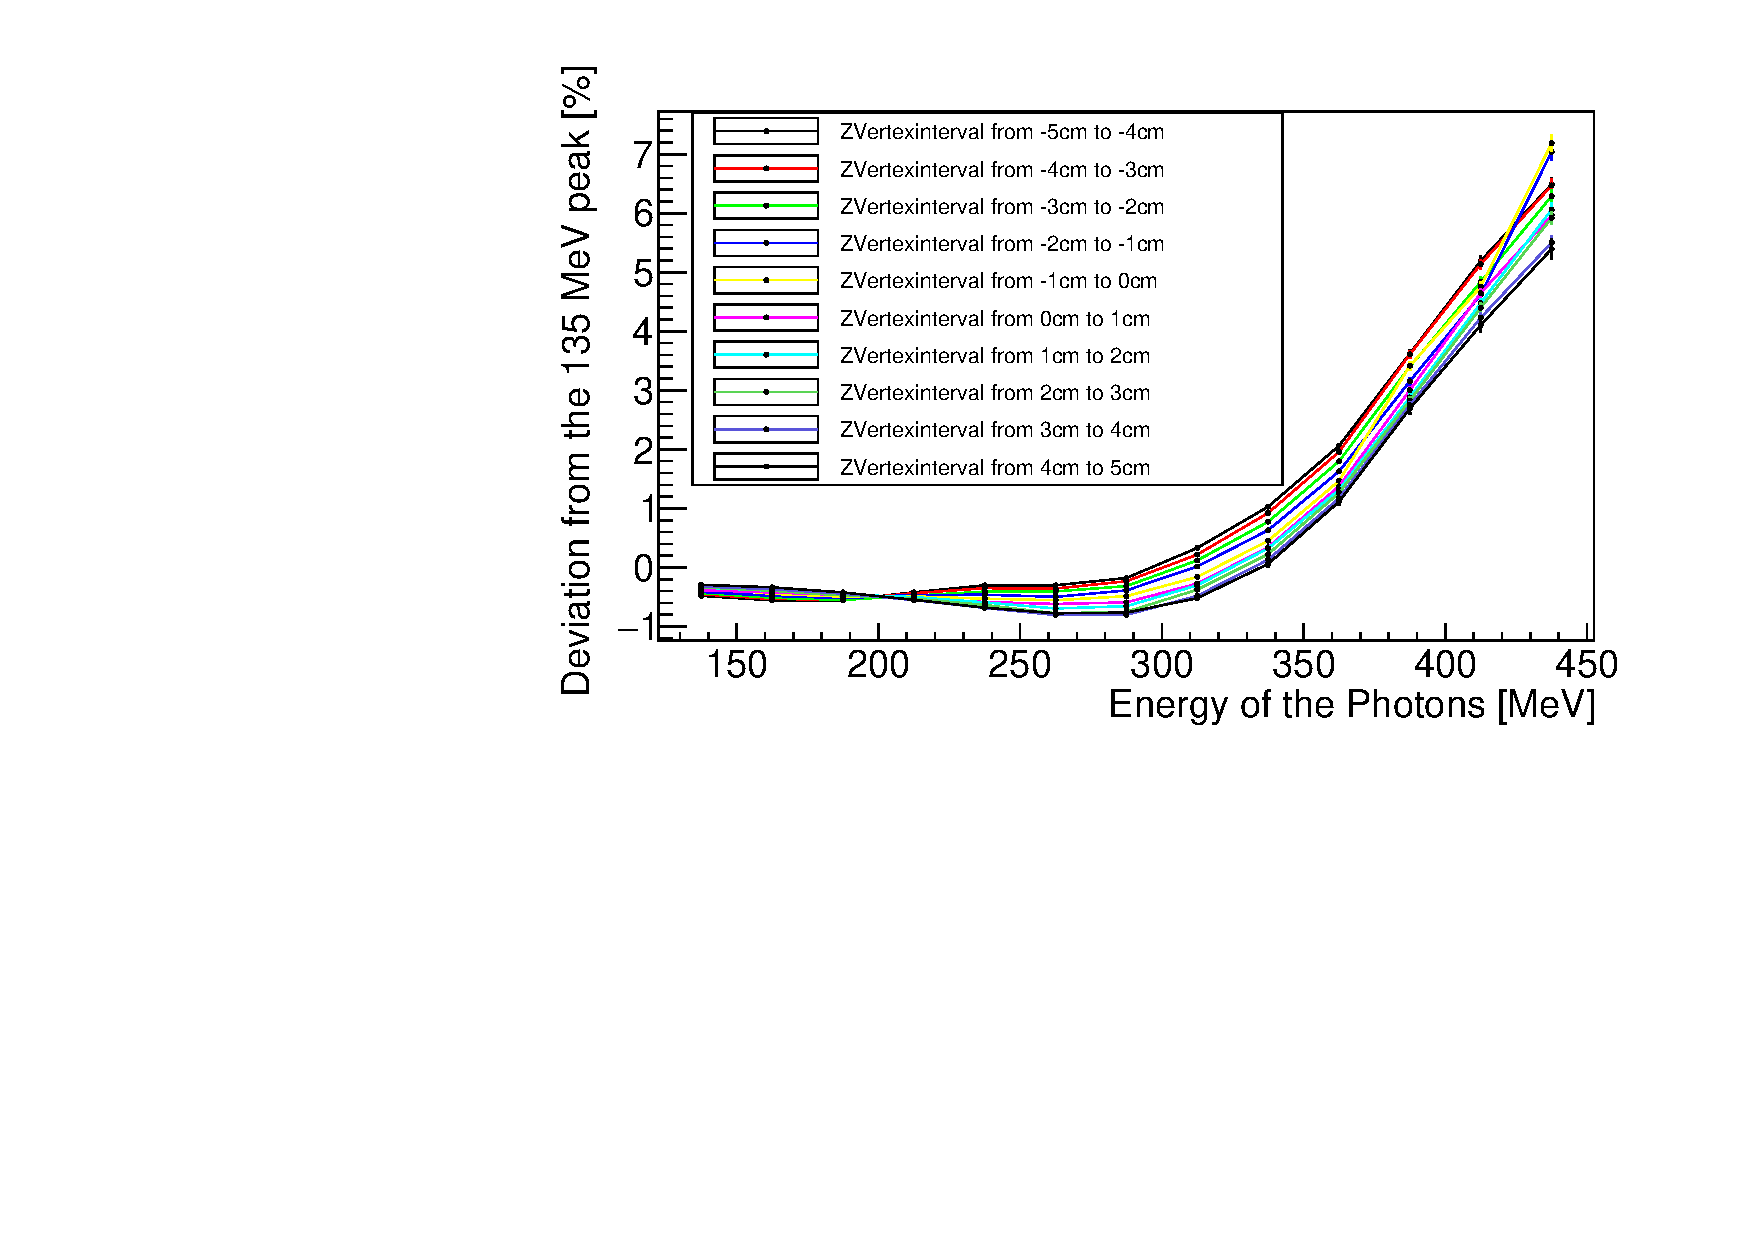
\includegraphics[width=100mm]{20172804MCZVertexDeviation}
		\caption[Simulation: Abweichung f\"ur verschiedene $z$-Vertices]{Daten aus der Simulation: Die Abweichung der $\pi^0$-Peak Position ist für verschiedene Intervalle des $z$-Vertex gegen die Energie der gemessenen Photonen. Es werden die Detektoren am Rand vernachl\"assigt. Die Energie der Photonen muss sich \"ahneln.}
		\label{fig:Z-Vertex-Multi-Graph}
	\end{center}
\end{figure}

Auch hier hat die Abweichung zwischen der errechneten invarianten Masse und der $\pi^0$ Masse die gleiche Form, wie in den vorherigen Abschnitten. So liegt nur eine geringe Abweichung f\"ur alle $z$-Vertices bei niedrigen Photonenenergien vor. Diese betr\"agt maximal etwa nur -0,5\%. 

Die Abweichungen treffen sich alle bei einer Energie von etwa $200\,\text{MeV}$. Dort haben alle $z$-Vertices eine Abweichung von etwa -0,5\%. An diesem Punkt erfolgt eine Vertauschung der Ordnung der $z$-Vertices. Vor $200\,\text{MeV}$ hat das Intervall von $4\,\text{cm}$ bis $5\,\text{cm}$ die gr\"o{\ss}te Abweichung und nach $200\,\text{MeV}$ hat es die kleinste. F\"ur das Intervall von $-4\,\text{cm}$ bis $-5\,\text{cm}$ gilt genau das Umgekehrte. Das liegt daran, dass f\"ur niedrige Photonenenergien auch das $\pi^0$ eine niedrige Energie besitzen muss. Das hei{\ss}t es ist wahrscheinlich, dass das $\pi^0$ in entgegengesetzter Richtung zum Strahl ausgesandt wird, da es sonst mehr Energie besitzen w\"urde. Somit kann es sein, dass die meisten gemessenen niederenergetischen Teilchen einen Polarwinkel besitzen, der gr\"o{\ss}er als 90$^{\circ}$ ist. Folglich wird der \"Offnungswinkel f\"ur $\pi^0$ die am Anfang des Targets entstehen, als zu gro{\ss} angenommen. F\"ur $\pi^0$ die am Ende des Targets entstehen wird, dann folglich ein zu kleiner \"Offnungswinkel gemessen. 

Bei einer Photonenenergie von \"uber $200\,\text{MeV}$ m\"ussen die $\pi^0$ ebenfalls mehr Energie besitzen. Folglich werden mehr $\pi^0$ in Strahlrichtung betrachtet und somit werden mehr Photonen ebenfalls in Strahlrichtung ausgesandt. Die Photonenenergie von $200\, \text{MeV}$ ist der Umkehrpunkt.
Ab hier wird f\"ur ein am Anfang des Targets entstehendes $\pi^0$ ein zu kleiner \"Offnungswinkel zwischen den ausgesandten Photonen gemessen und umgekehrt.

Ab $200\,\text{MeV}$ f\"achert sich die Abweichung auch immer weiter auf. Bei $450\,\text{MeV}$ betr\"agt sie fast 2\%. Das wiederum bedeutet, dass die r\"aumliche Ausdehnung des Target nur einen kleinen Effekt, im Gegensatz zur bereits festgestellten Abweichung besitzt.

Die maximale Abweichung wird ebenfalls bei $450\,\text{MeV}$ erreicht und betr\"agt ca. 7\%.

Die Ursache der Auff\"acherung wird nochmal genauer in Kapitel \ref{sec:Unterschied-Oeffnungswinkel-ZVertex} beschrieben.
%Auch hier hat die Abweichung der errechneten invarianten Masse zur $\pi^0$-Masse die gleiche Form. So lag nur eine geringe Abweichung für niedrige Photonenenergien vor. Diese nahm im Energieintervall von 125 MeV bis 200 MeV leicht zu. In diesem Intervall liegen die Abweichungen für verschiedene Z-Vertices sehr nahe beieinander. Im nächsten Photonenenergieintervall von 200 MeV bis 300 MeV nahm die Abweichung für Intervalle nahe Strahleneingang sehr schwach zu, während sie für Intervalle in der Nähe vom Strahlenausgang fast konstant blieb. Dadurch wurden die einzelnen Linien aufgefächert. Ab 300 MeV nahm die Abweichung wieder für alle Z-Vertices gleichmäßig zu, sodass sie nicht weiter aufgefächert wurden. Die maximale Abweichung von fast 9\% erreichte man bei einer Photonenenergie von 450 MeV, wenn man das Z-Vertex-Intervall von -5\,\text{cm}$ bis -4\,\text{cm}$ betrachtete. Dies ist nicht weiter verwunderlich, da die meisten Teilchen für hohe Photonenenergien in der Nähe des Strahlenausgangs detektiert werden. (Siehe dazu \ref{sec:Vernachlaessigung-der-Detektoren-am-Rand}) Betrachtet man nun ein Z-Vertex-Intervall in der Nähe des Strahlenausgangs, so ist der tatsächliche Öffnungswinkel zwischen den beiden detektierten Photonen als der berechnete. Daraus folgt mit Gleichung zur Berechnung der invarianten Masse \ref{eq:Formel-zur-Berechnung-der-invarianten-Masse}, dass die berechnete invariante Masse größer, als die tatsächliche ist. Für das Z-Vertex-Intervall von 4 cm bis 5 cm erreichte man bei einer Photonenenergie von 450 MeV eine Abweichung von etwa 7,5\%. Das heißt die Auffächerung betrug nur etwas mehr als 1\%. Das wiederum bedeutete, dass die räumliche Ausdehnung des Targets keinen allzu großen Effekt auf die Abweichung hat.

%Wie zu erwarten war, ergaben verschiedene Z-Vertices unterschiedliche Abweichungen des Peaks. So war die Abweichung gr\"o{\ss}er, wenn die Bedingung galt, dass das $\pi^0$ am Rand des Targets zerf\"allt, als wenn nur Zerf\"alle in der Mitte des Targets betrachtet wurden. Dies lag daran, das zur Kalibrierung des Crystal-Ball angenommen wurde, dass das Meson im Zentrum des Targets zerf\"allt. Das hatte zur Folge, dass der Winkel aus Gleichung \ref{eq:Formel-zur-Berechnung-der-invarianten-Masse} verf\"alscht wurde, wenn ein Zerfall au{\ss}erhalb des Zentrum des Targets betrachtet wurde. Der Grund daf\"ur war, dass beim Zerfall des $\pi^0$ die meisten hochenergetischen Photonen in Strahlrichtung entstehen\footnote{Siehe dazu Kapitel \ref{sec:Vernachlaessigung-der-Detektoren-am-Rand} Ende}. Folglich hoben sich die Abweichungen im Winkel nicht mit der Statistik weg, sondern es gab eine inhomogene Verteilung der Winkel. Auch zu sehen ist, dass der Abstand der Linien f\"ur niedrige Energie, fast durchgehend, ca. 1\% betrug, ausgenommen ist das Intervall von -5 cm bis -4 cm. Ebenfalls war zu erkennen, dass die einzelnen Abweichungen sich f\"ur gr\"o{\ss}ere Energien der ca. 2\% Abweichung ann\"aherten. Eine solche Abweichung war bereits in Kapitel \ref{sec:Reelle-Daten} zu erkennen, dort wurde der Z-Vertex nicht in Intervalle unterteilt, sondern als ganzes betrachtet.

%Da auch in den simulierten Daten diese Abweichung der $\pi^0$-Peak Position zu erkennen war, musste genauer nach der Ursache gesucht werden.




\subsection{Unterschied zwischen generierten und berechneten Winkeln}
\label{sec:Unterschied-tatsaechlicher-gemessener-Winkel}

Es gibt die Vermutung, dass ein starker Unterschied, zwischen dem gemessenen und dem tatsächlichem Öffnungswinkel der beiden Photonen vorliegt.

Die Detektoren des Crystal-Balls sollen alle so ausgerichtet sein, dass sie in die Richtung des Zentrum des Targets zeigen, dieser liegt im Mittelpunkt der Kugel. Ist dies nicht der Fall, so wird ein falscher Öffnungswinkel zwischen den beiden Photonen bestimmt und damit nach Gleichung \ref{eq:Formel-zur-Berechnung-der-invarianten-Masse} eine falsche invariante Masse.

Um diesen Unterschied zu untersuchen, wird zuerst überprüft, ob ein von Null verschiedener Winkel zwischen dem generierten und dem gemessenen Teilchen vorliegt.

Dafür muss bestimmt werden, welches generierte Teilchen zu welchem gemessenem gehört. Dazu h\"alt man ein generiertes Teilchen fest und bestimmt anschließend den Winkel zwischen ihm und jedem gemessenen Teilchen. Wenn der Winkel am kleinsten ist, dann handelt es sich wahrscheinlich um das gleiche Teilchen. Danach wird dies für das nächste generierte Teilchen durchgeführt. Da der Crystal-Ball nicht den gesamten Raum abdeckt, sondern \"Offnungen ohne Detektoren besitzt, werden auch hier die Detektoren am Rand vernachlässigt. In den vorherigen Abschnitten mit Simulation kann kein Unterschied zwischen Berücksichtigung und Vernachlässigung der Detektoren am Rand festgestellt werden, folglich k\"onnen sie ohne große Bedenken vernachlässigt werden. Dies hat einen weiteren Vorteil. Dadurch k\"onnen generierte Photonen, welche einen zu kleinen bzw. zu großen $\theta$ Winkel besitzen und damit nicht mehr im Crystal-Ball detektiert werden k\"onnen, direkt verworfen werden. Das führt dazu, dass jedes generierte Photon auch im Crystal-Ball gemessen werden. Gäbe es diese Bedingung nicht, so würde ein generiertes Photon, welches nicht im Crystal-Ball detektiert wird, mit einem anderen Teilchen gleichgesetzt, da der Winkel zwischen diesen am kleinsten wäre. Dies würde das Ergebnis verfälschen. 

\begin{figure}[h!]
\begin{center}
$\begin{array}{cc}

		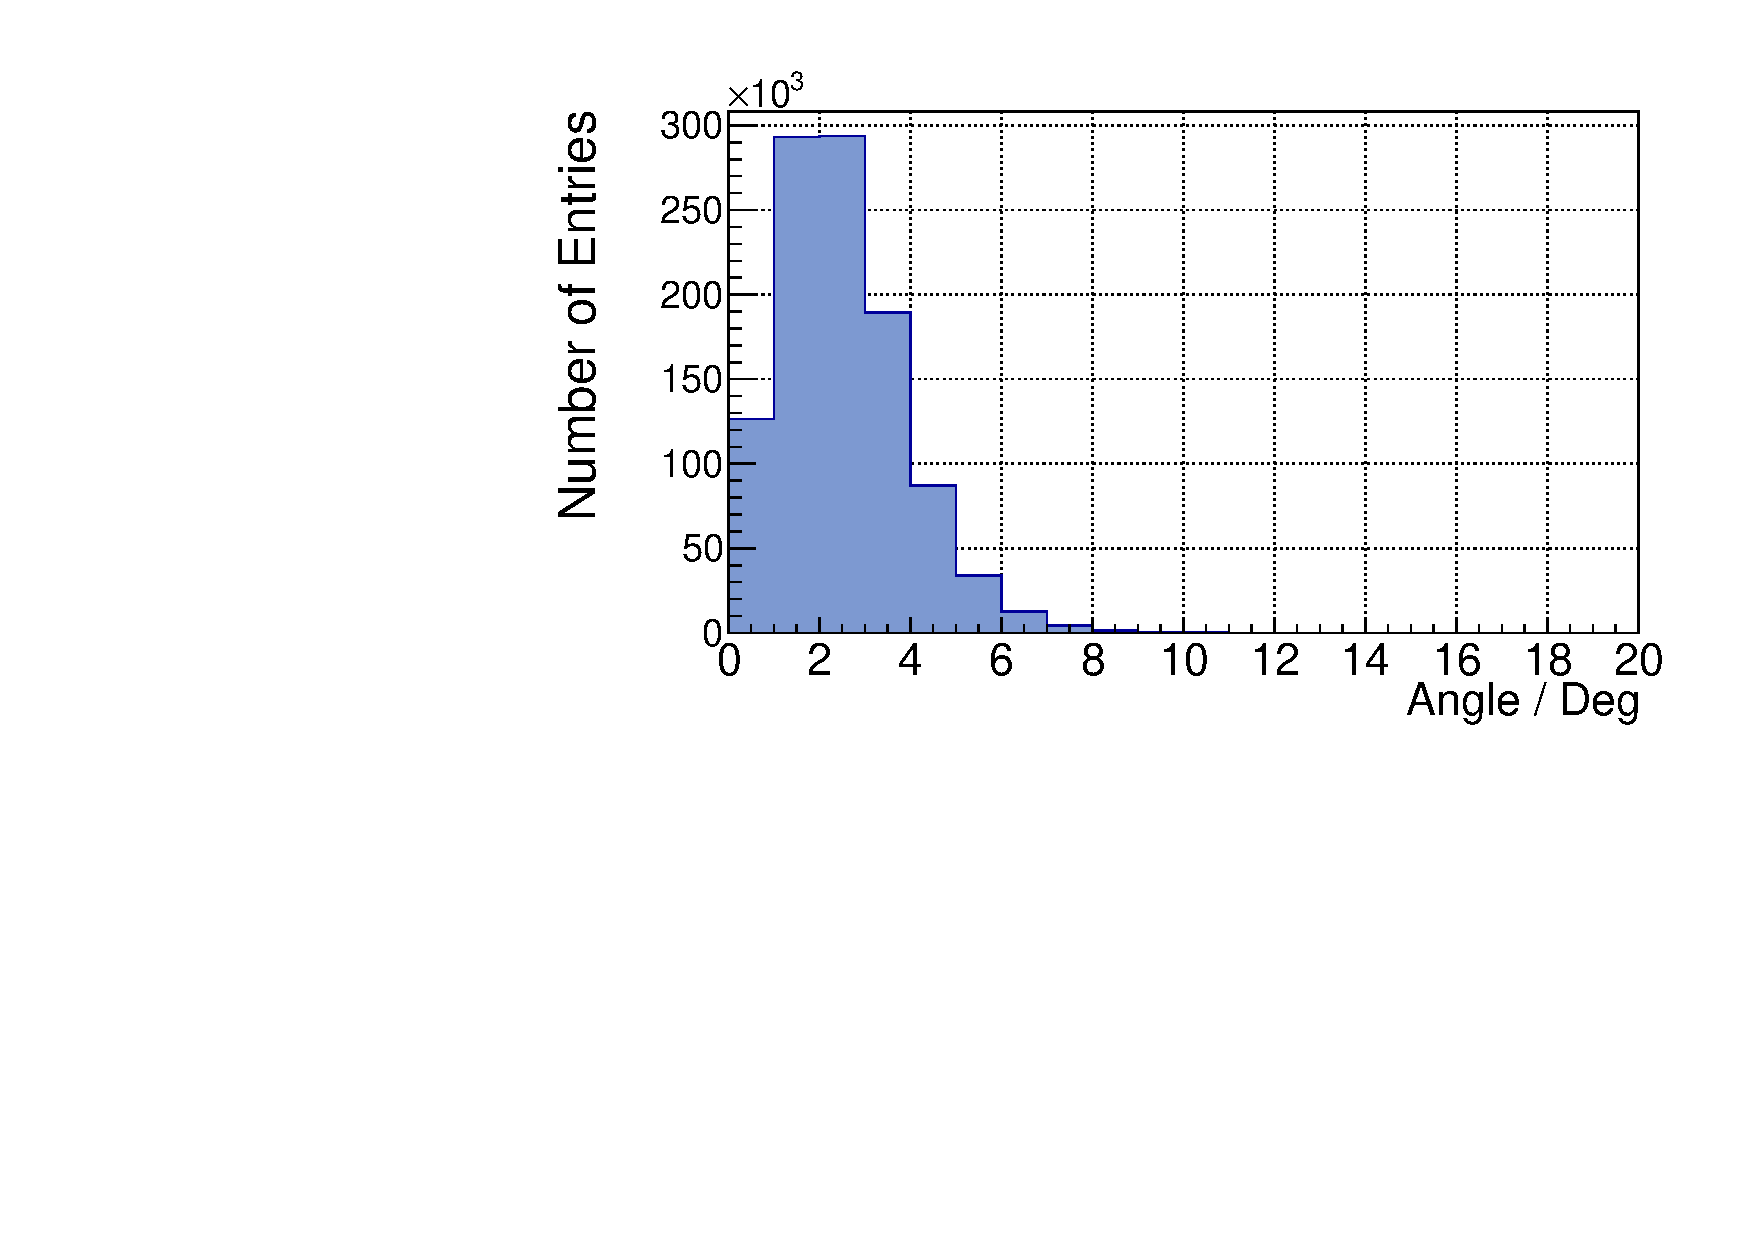
\includegraphics[width=74mm]{AngleRegGen/20172604AngleRegGen100-125MeV}
		

		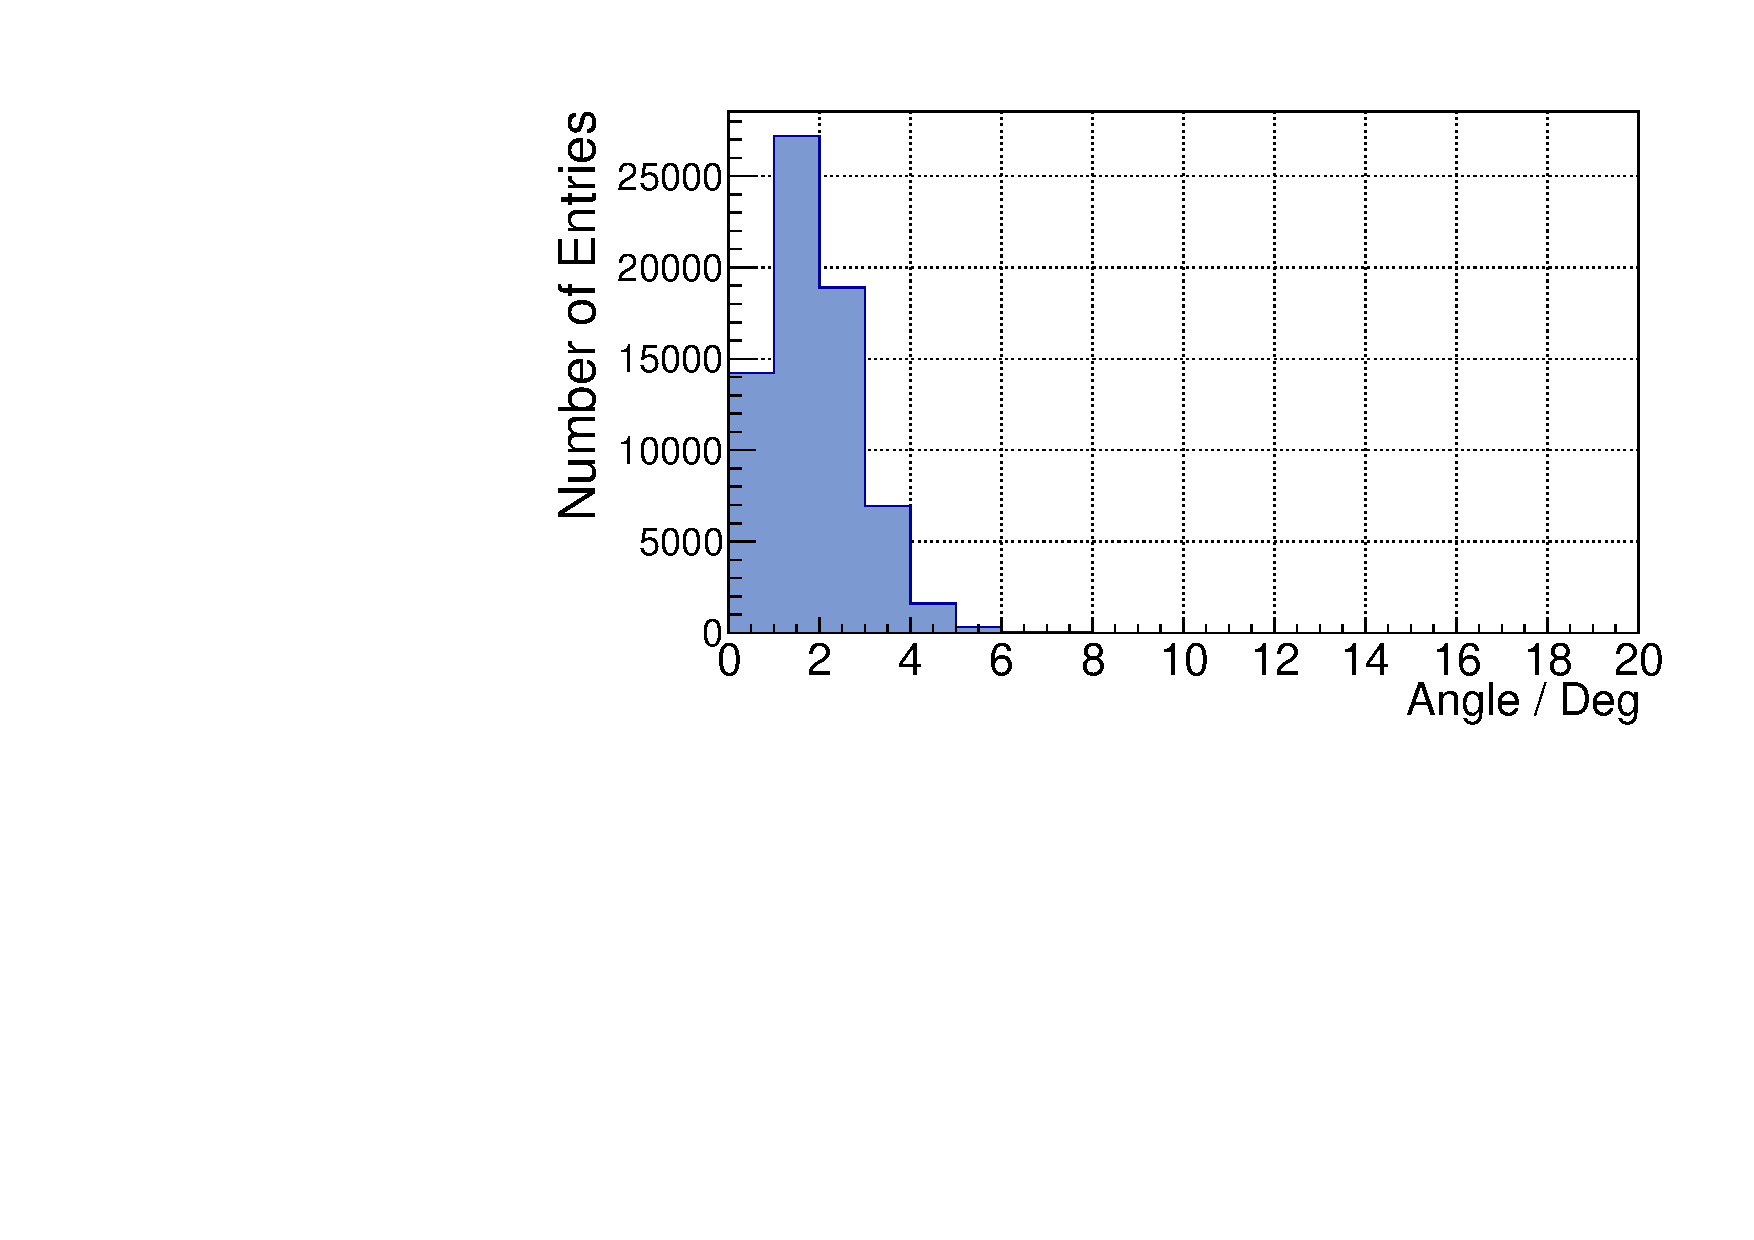
\includegraphics[width=74mm]{AngleRegGen/20172604AngleRegGen400-425MeV}
\end{array}$
\end{center}
	\caption[Simulation: Winkel zw. Gen. und Rec. Photonen]{Daten aus der Simulation: Es wird ein langes Target benutzt. Der Winkel zwischen dem generiertem und dem rekonstruiertem Photon ist gegen verschiedene Photonenenergien aufgetragen. Die Energie der Photonen muss sich \"ahneln. Links besitzen die Photonen eine Energie von $125\,\text{MeV}$ bis $150\,\text{MeV}$, w\"ahrend sie rechts eine Energie von $425\,\text{MeV}$ bis $450\,\text{MeV}$ besitzen. Das vollst\"andige 2D-Histogramm ist in Abbildung \ref{fig:Angle-Rec-Gen-Hist} zu sehen.}
	\label{fig:Winkel-Gen-Rec}

\end{figure}


In Abbildung \ref{fig:Winkel-Gen-Rec} ist der Winkel zwischen dem generierten Photon und dem gemessenen Photon gegen die Energie des gemessenen aufgetragen.  

Links besitzen die Photonen eine Energie von $125\,\text{MeV}$ bis $150\,\text{MeV}$, w\"ahrend sie rechts in der Abbildung $425\,\text{MeV}$ bis $450\,\text{MeV}$ besitzen. Man erkennt, dass f\"ur gr\"o{\ss}ere Energien, der Winkel zwischen dem generiertem Photon und dem rekonstruiertem Photon kleiner wird.

Dies l\"asst sich dadurch erkl\"aren, dass h\"oher energetische Photonen einen deutlich st\"arkeren Schauer ausl\"osen, als Photonen mit niedrigerer Energie. Das f\"uhrte dazu, dass auch der Schauerradius gr\"o{\ss}er wird. Dadurch werden mehr Detektorkristalle ausgel\"ost, wodurch sich der genaue Auftreffort des Photons pr\"aziser bestimmen l\"asst. Folglich nimmt der Winkel zwischen dem generiertem und dem entsprechendem gemessenem Photonen mit zunehmender Energie ab.

Da nun bekannt ist, dass es einen Winkel zwischen generierten und gemessenen Photonen gibt, wird nun direkt der \"Offnungswinkel zwischen den beiden generierten und den beiden gemessenen Photonen verglichen.
Dazu wird die Abweichung der beiden \"Offnungswinkel berechnet.

\begin{equation}
	\Delta\alpha = \alpha_{\text{rec}} - \alpha_{\text{gen}}
\end{equation}


 Dazu wird vom rekonstruiertem \"Offnungswinkel $\alpha_{\text{rec}}$ der generierte $\alpha_{\text{gen}}$ abgezogen. Die Differenz wird dann $\Delta\alpha$ gesetzt. Dieses wird dann f\"ur verschiedene Photonenenergien in ein Histogramm aufgetragen.
%\begin{figure}[h!]
%	\centering
%	\begin{minipage}{0.45\textwidth}
%		\centering
%		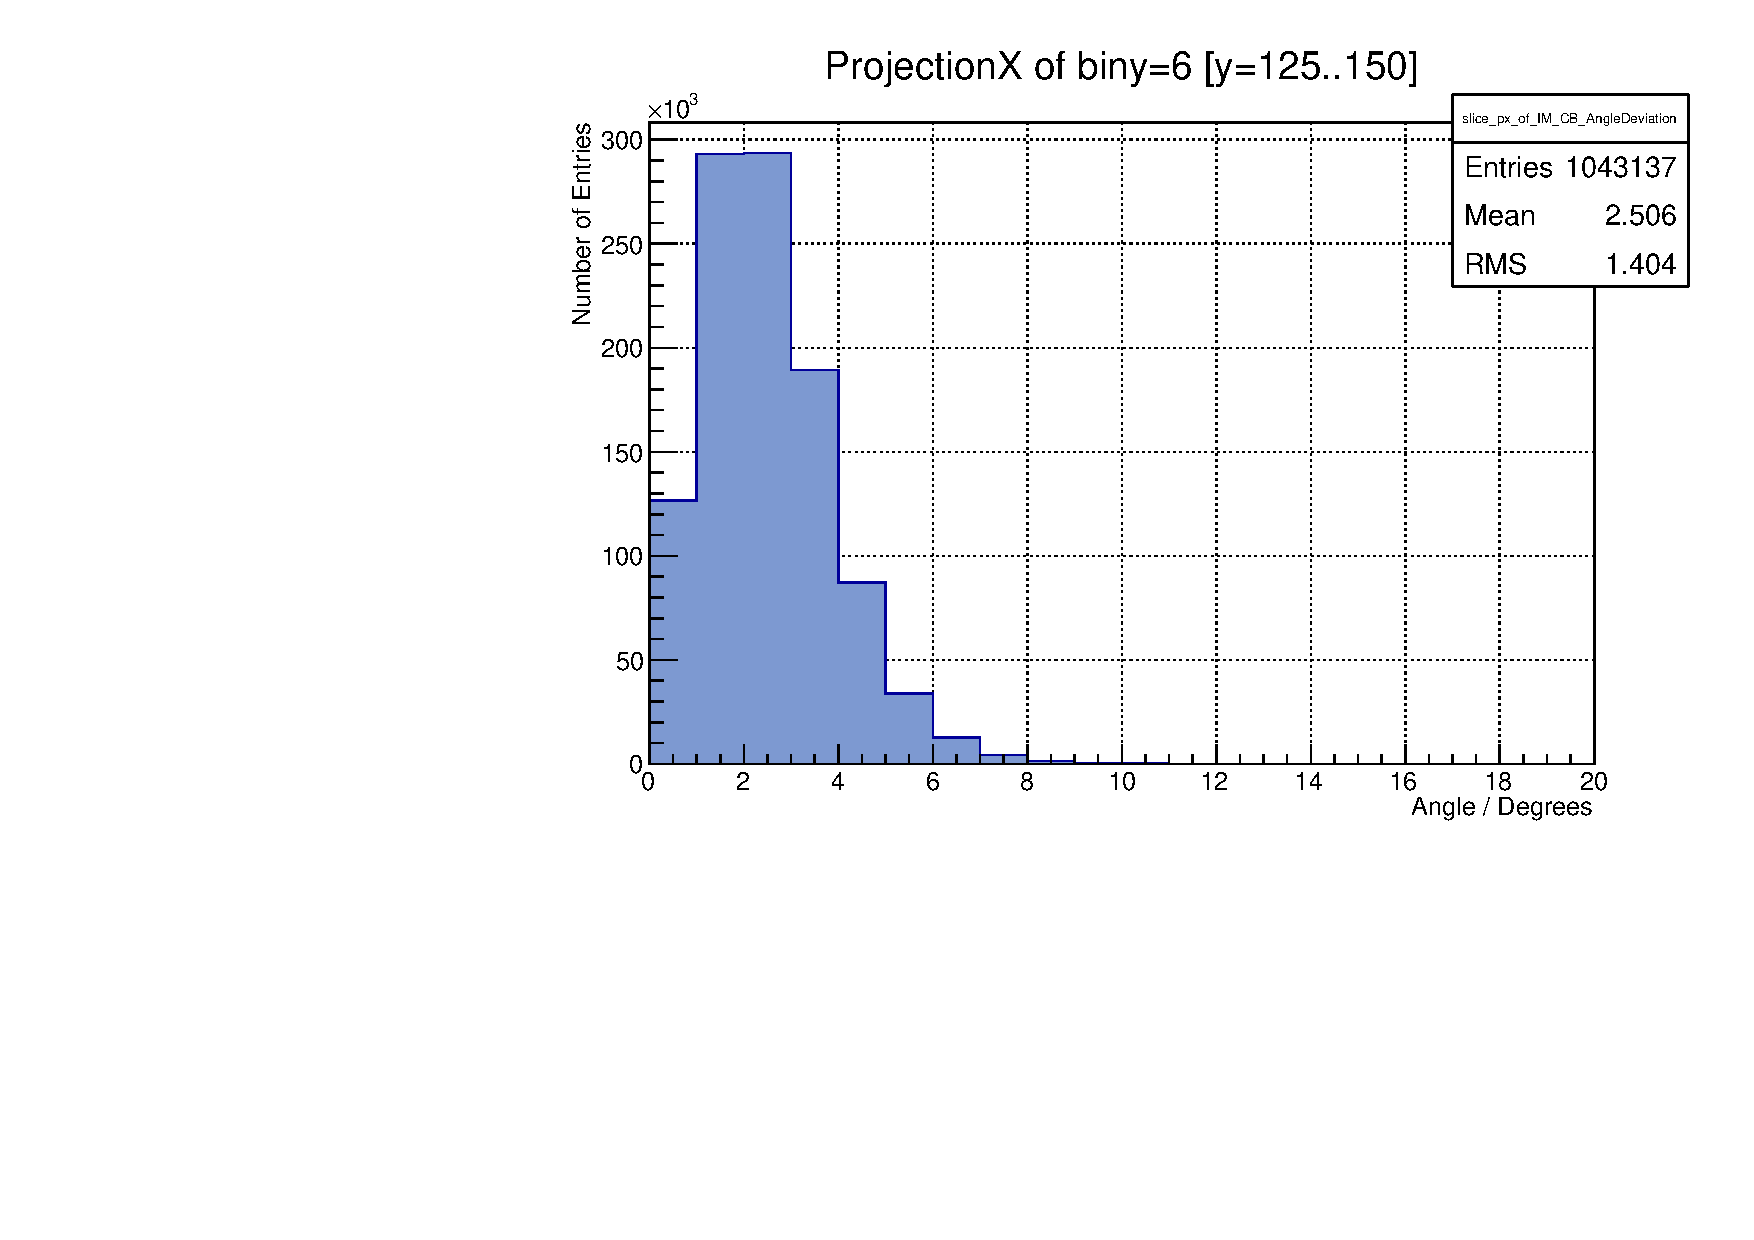
\includegraphics[width=0.9\textwidth]{20171804MCTrueCandidatsAngleDeviation125MeV}
%		
%	\end{minipage}
%	\hfill
%	\begin{minipage}{0.45\textwidth}
%		\centering
%		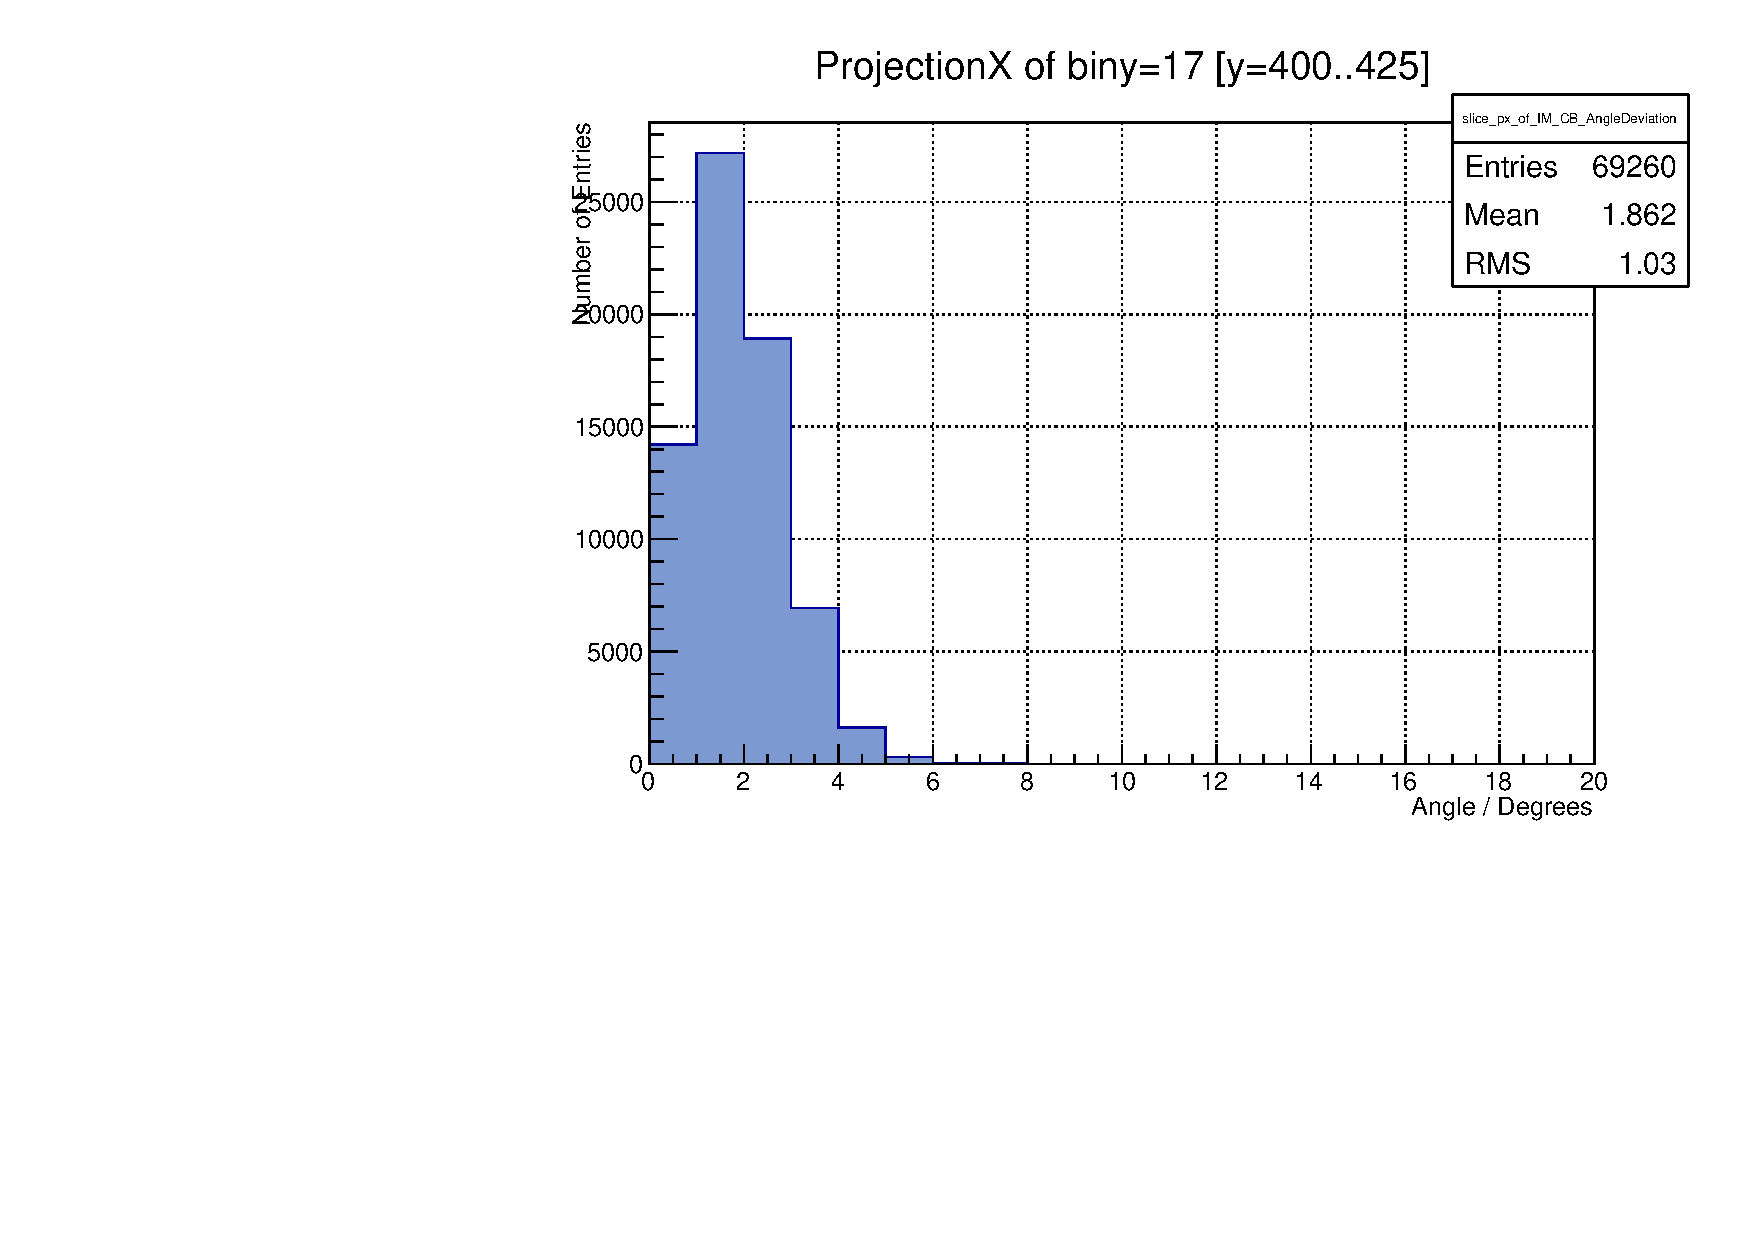
\includegraphics[width=0.9\textwidth]{20171804MCTrueCandidatsAngleDeviation400MeV}
%	\end{minipage}
%	\caption{Abweichung in Grad f\"ur verschiedene Energieintervalle. Links besa{\ss}en die detektierten Photonen eine Energie zwischen 125 MeV bis 150 MeV, rechts 400 MeV bis 425 MeV.}
%	\label{fig:Abweichung-Winkel-ge-rec-verschiedene-Energien}
%	
%\end{figure}
\begin{figure}[h!]
\begin{center}
	$\begin{array}{cc}
	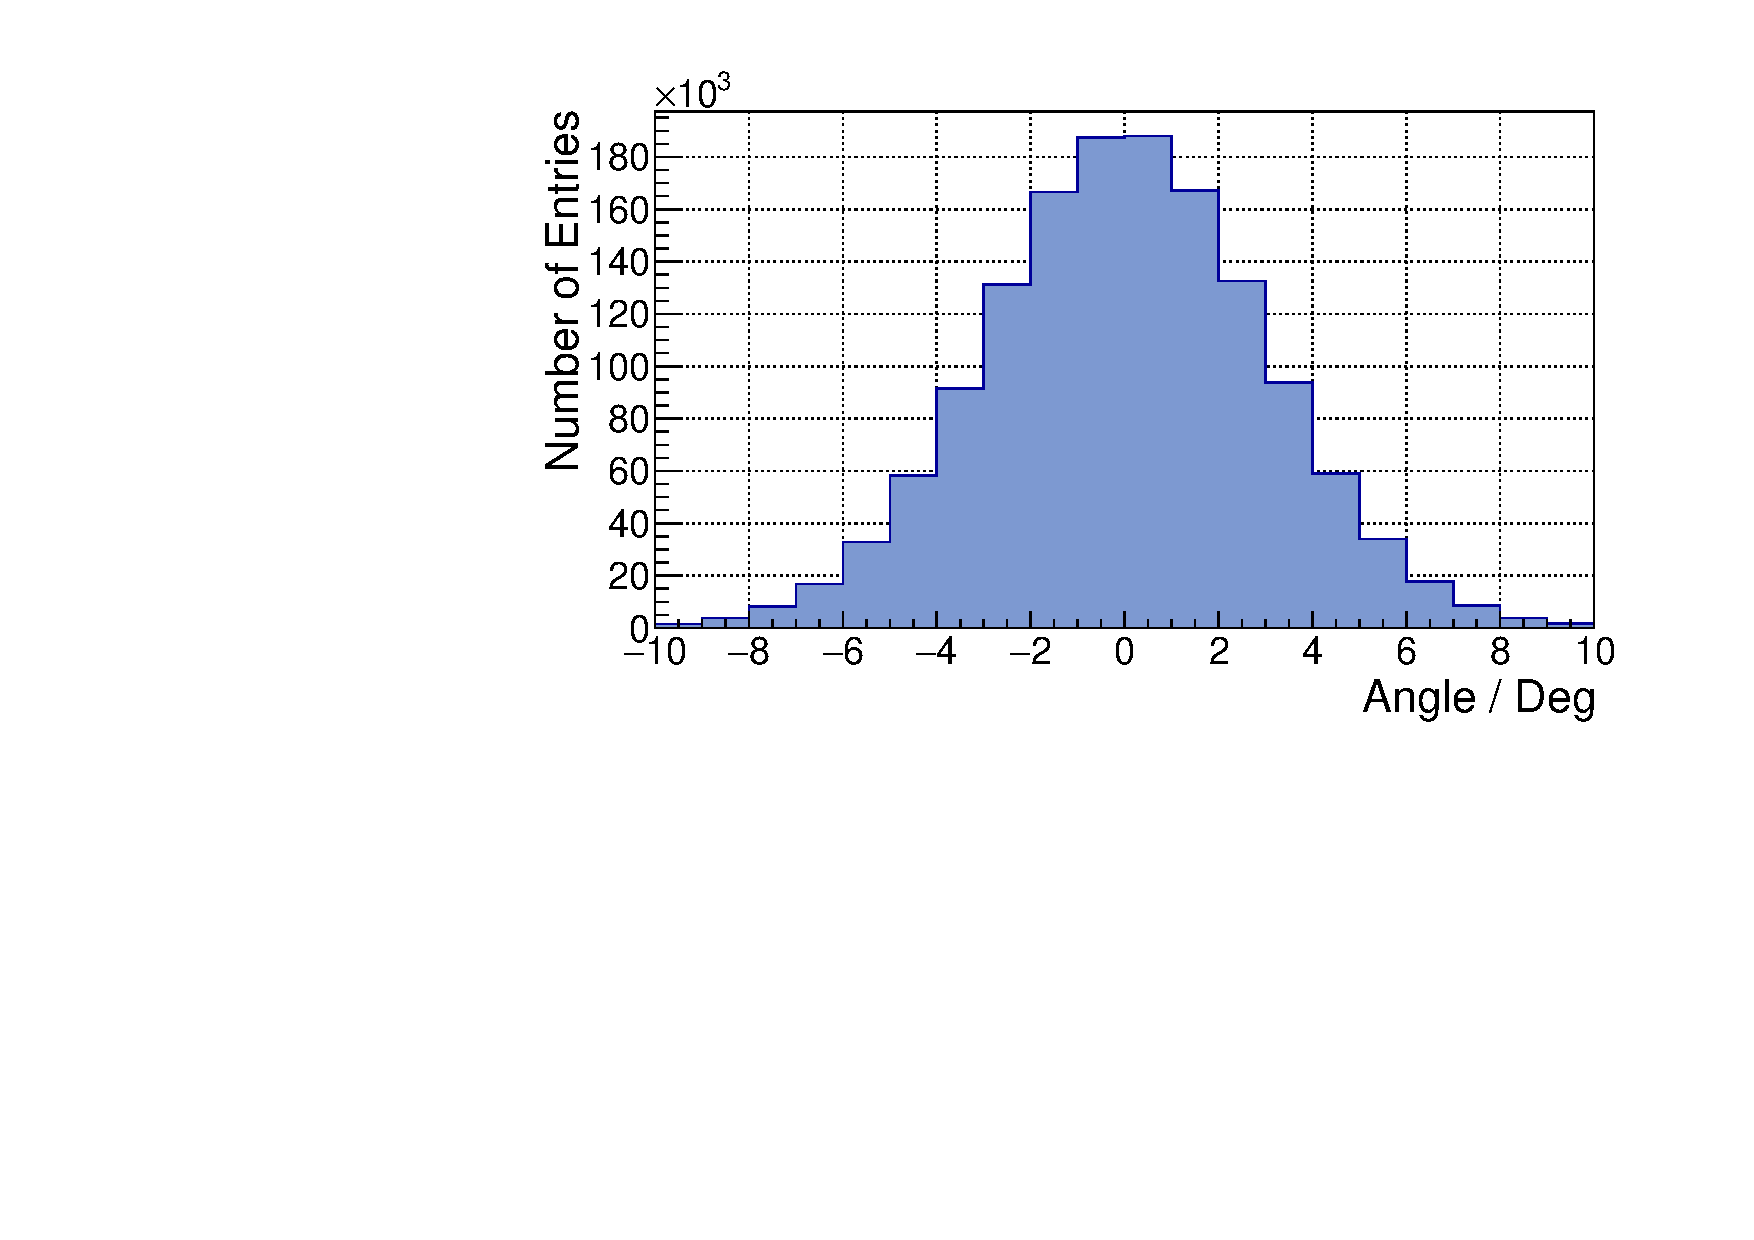
\includegraphics[width=74mm]{AngleRegGen/20172704MCDeviationOpeningAngle125MeV}
	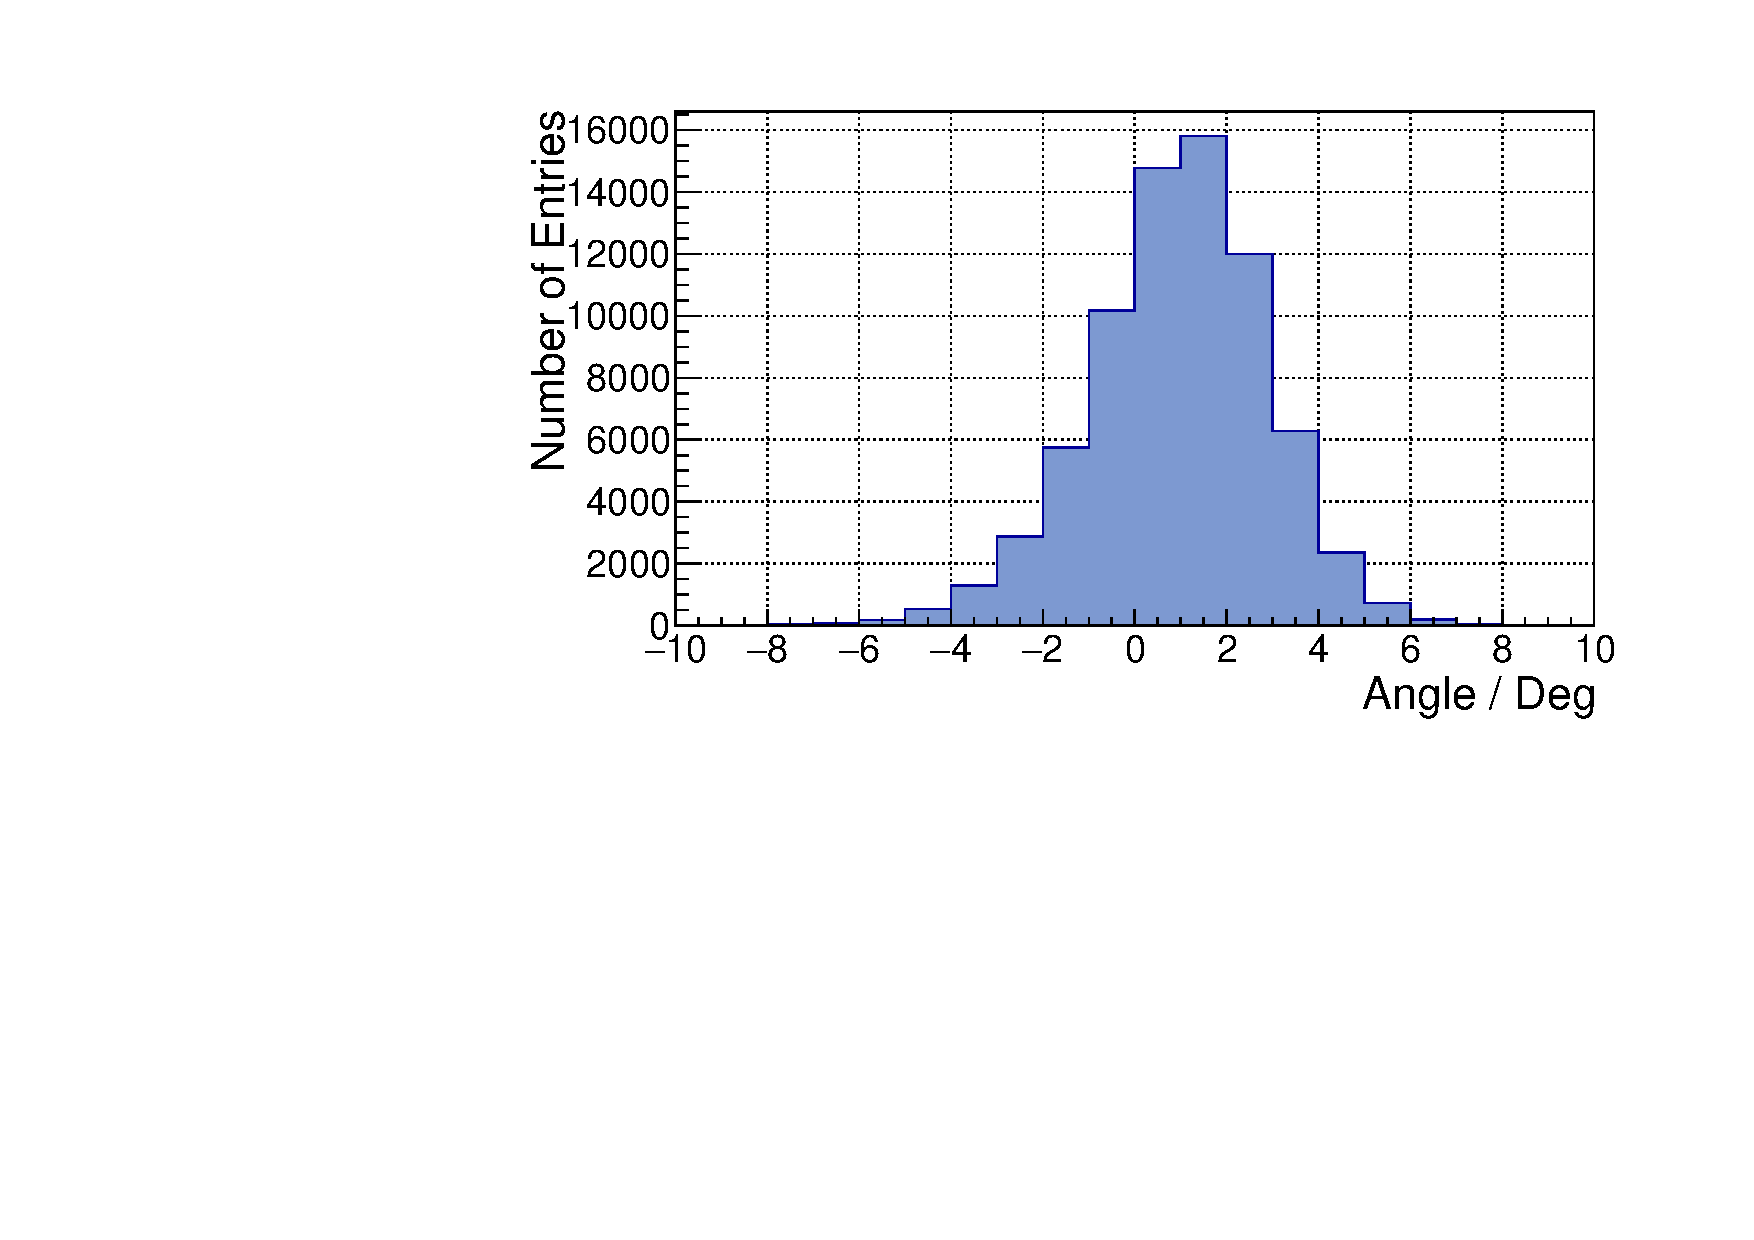
\includegraphics[width=74mm]{AngleRegGen/20172704MCDeviationOpeningAngle400MeV}
	\end{array}$
	\caption[Simulation: Unterschied zwischen gen. und rek. \"Offnungswinkel]{Daten aus der Simulation: Aufgetragen ist $\Delta\alpha$. Links liegt die Energie der Photonen zwischen $125\,\text{MeV}$ und $150\,\text{MeV}$, rechts zwischen $425\,\text{MeV}$ und $450\,\text{MeV}$.}
	\label{fig:Abweichung-Winkel-Oeffnungswinkel}
\end{center}
\end{figure}

In Abbildung \ref{fig:Abweichung-Winkel-Oeffnungswinkel} ist diese Abweichung f\"ur zwei verschiedene Energien zu sehen. Links besitzen die Photonen eine Energie von $125\,\text{MeV}$ bis $150\,\text{MeV}$, w\"ahrend sie rechts eine Energie von $425\,\text{MeV}$ bis $450\,\text{MeV}$ besitzen. Hier erkennt man, dass f\"ur kleine Energien die Abweichung der beiden \"Offnungswinkel um die Null verteilt ist. Liegt allerdings eine hohe Photonenenergie vor, so verschiebt sich diese Verteilung etwas nach rechts, sodass die h\"aufigste Differenz bei $1^{\circ} \textnormal{ bis } 2^{\circ}$ liegt. Das bedeutet in der Regel wird ein zu gro{\ss}er \"Offnungswinkel f\"ur hohe Photonenenergien rekonstruiert. Mit der Gleichung zur Berechnung der invarianten Masse (Gleichung \ref{eq:Formel-zur-Berechnung-der-invarianten-Masse}) folgt damit, das eine zu gro{\ss}e invariante Masse berechnet wird.

Betrachtet man nun noch einmal die beiden Plots in Abbildung \ref{fig:True-OpeningAngle}, so f\"allt auf, dass bei einer Photonenenergie von $450\,\text{MeV}$ ein \"Offnungswinkel von nur 17$^{\circ}$ vorliegt. Bei einem so kleinen \"Offungswinkel schafft es der Algorithmus zur Clusterbildung nicht mehr eindeutig zwischen zwei registrierten Events zu unterscheiden. 





%Das vollst\"andige Histogramm ist in Abbildung \ref{fig:Unterschied-Rec-Gen-Opening-Angle} zu sehen. Daraus folgte, dass der \"Offnungswinkel f\"ur hohe Energien relativ genau bestimmt werden konnte. Das bedeutete allerdings, dass die Abweichungen der errechneten invarianten Masse zur tats\"achlichen Masse des $\pi^0$ dadurch nicht erkl\"art werden konnten, da diese mit steigender Photonenenergie zunahm. 
 
 


\subsection{Unterschied zwischen generierten und berechneten \"Offnungswinkel f\"ur verschiedene $z$-Vertices}
\label{sec:Unterschied-Oeffnungswinkel-ZVertex}

In Abschnitt \ref{sec:Z-Vertex-Abhaengigkeit} wurde bereits gezeigt, dass eine Abh\"angigkeit zwischen dem Ort des Zerfalls und dem \"Offnungswinkel vorliegt. Dies soll in diesem Abschnitt weiter untersucht werden. Dazu wird das Target wieder in ein Zentimeter lange Abschnitte unterteilt, welche einzeln untersucht und anschlie{\ss}end verglichen werden.

Das erste Intervall, welches betrachtet wird liegt am Anfang des Targets und hat somit einen $z$-Vertex von $z=-5\,\text{cm}$ bis $z=-4\,\text{cm}$. Das zweite Intervall liegt im Ursprung, das hei{\ss}t der $z$-Vertex liegt in einem Intervall von $z= -0.5\,\text{cm}$ bis $z = 0.5\,\text{cm}$. Das letzte Intervall, welches hier betrachtet wird, liegt am Ende des Target und besitzt damit einen $z$-Vertex von $z= 4\,\text{cm}$ bis $z= 5\,\text{cm}$.
Auch hier wird von dem rekonstruiertem \"Offnungswinkel der generierte abgezogen.


\begin{figure}[h!]
	\begin{center}
		\text{Anfang des Targets:}
		$		
		\begin{array}{cc}
		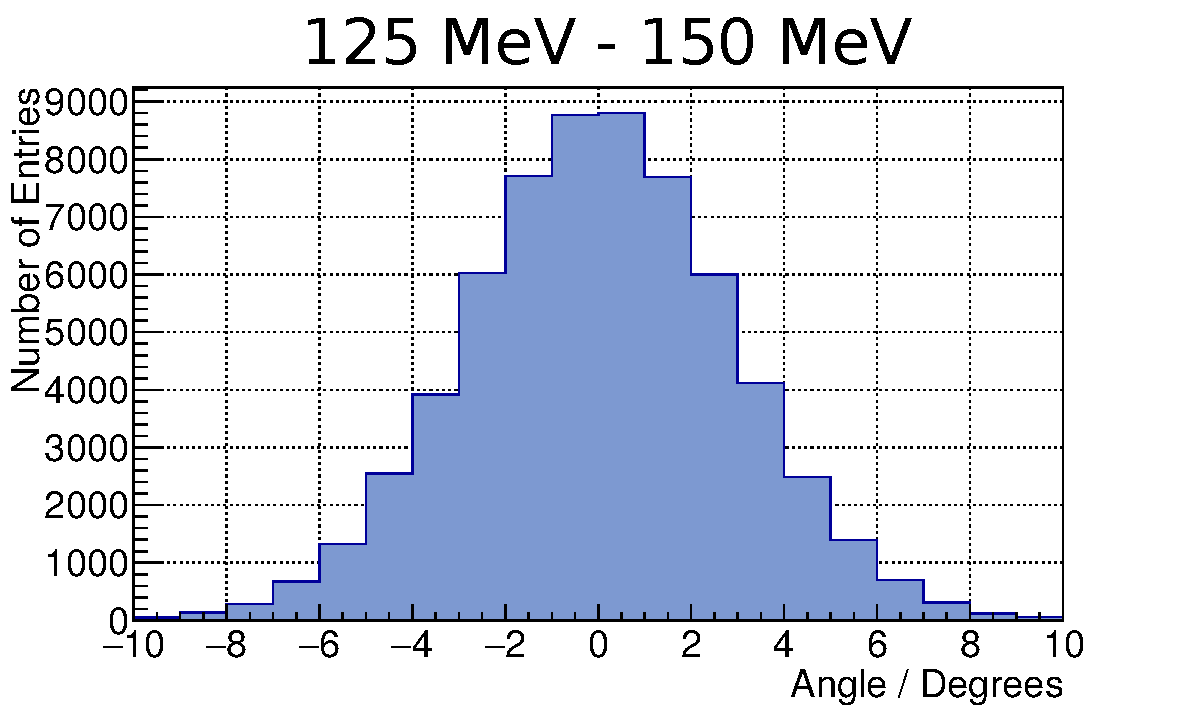
\includegraphics[width=74mm]{OeffZVertex/20170205DiffOeffZVertex-4_125MeV}
		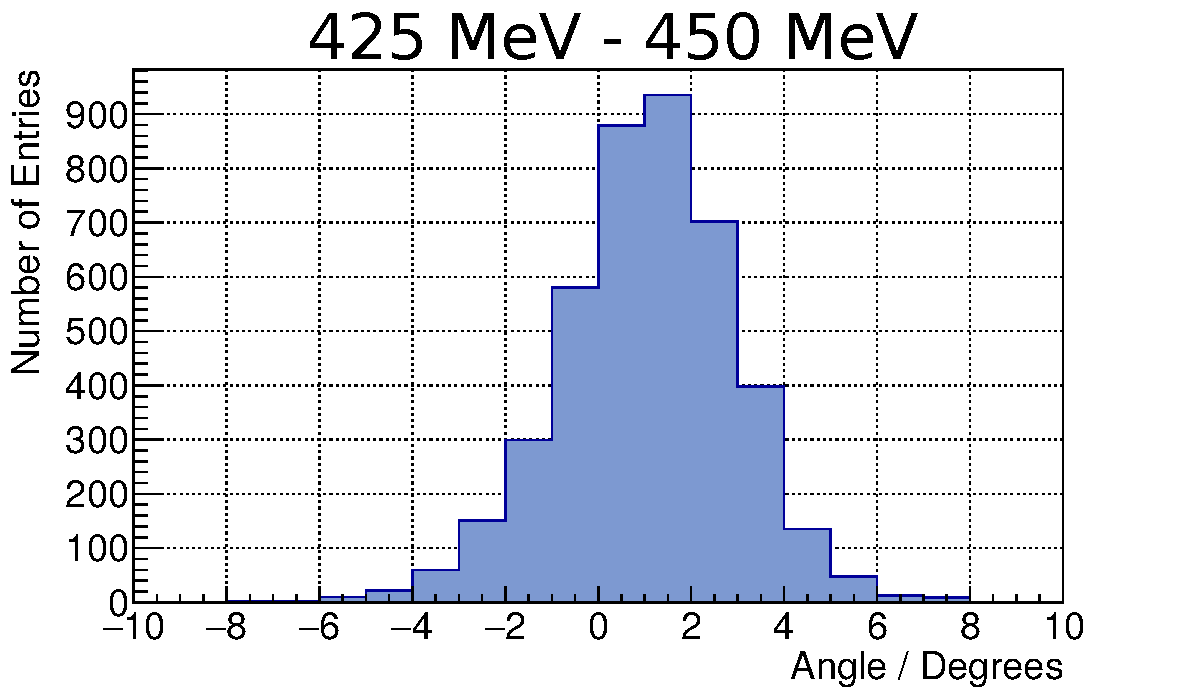
\includegraphics[width=74mm]{OeffZVertex/20170205DiffOeffZVertex-4_425MeV}
		
		\end{array}$
	\end{center}

\begin{center}
	\text{Mitte des Targets:}
	$\begin{array}{cc}
	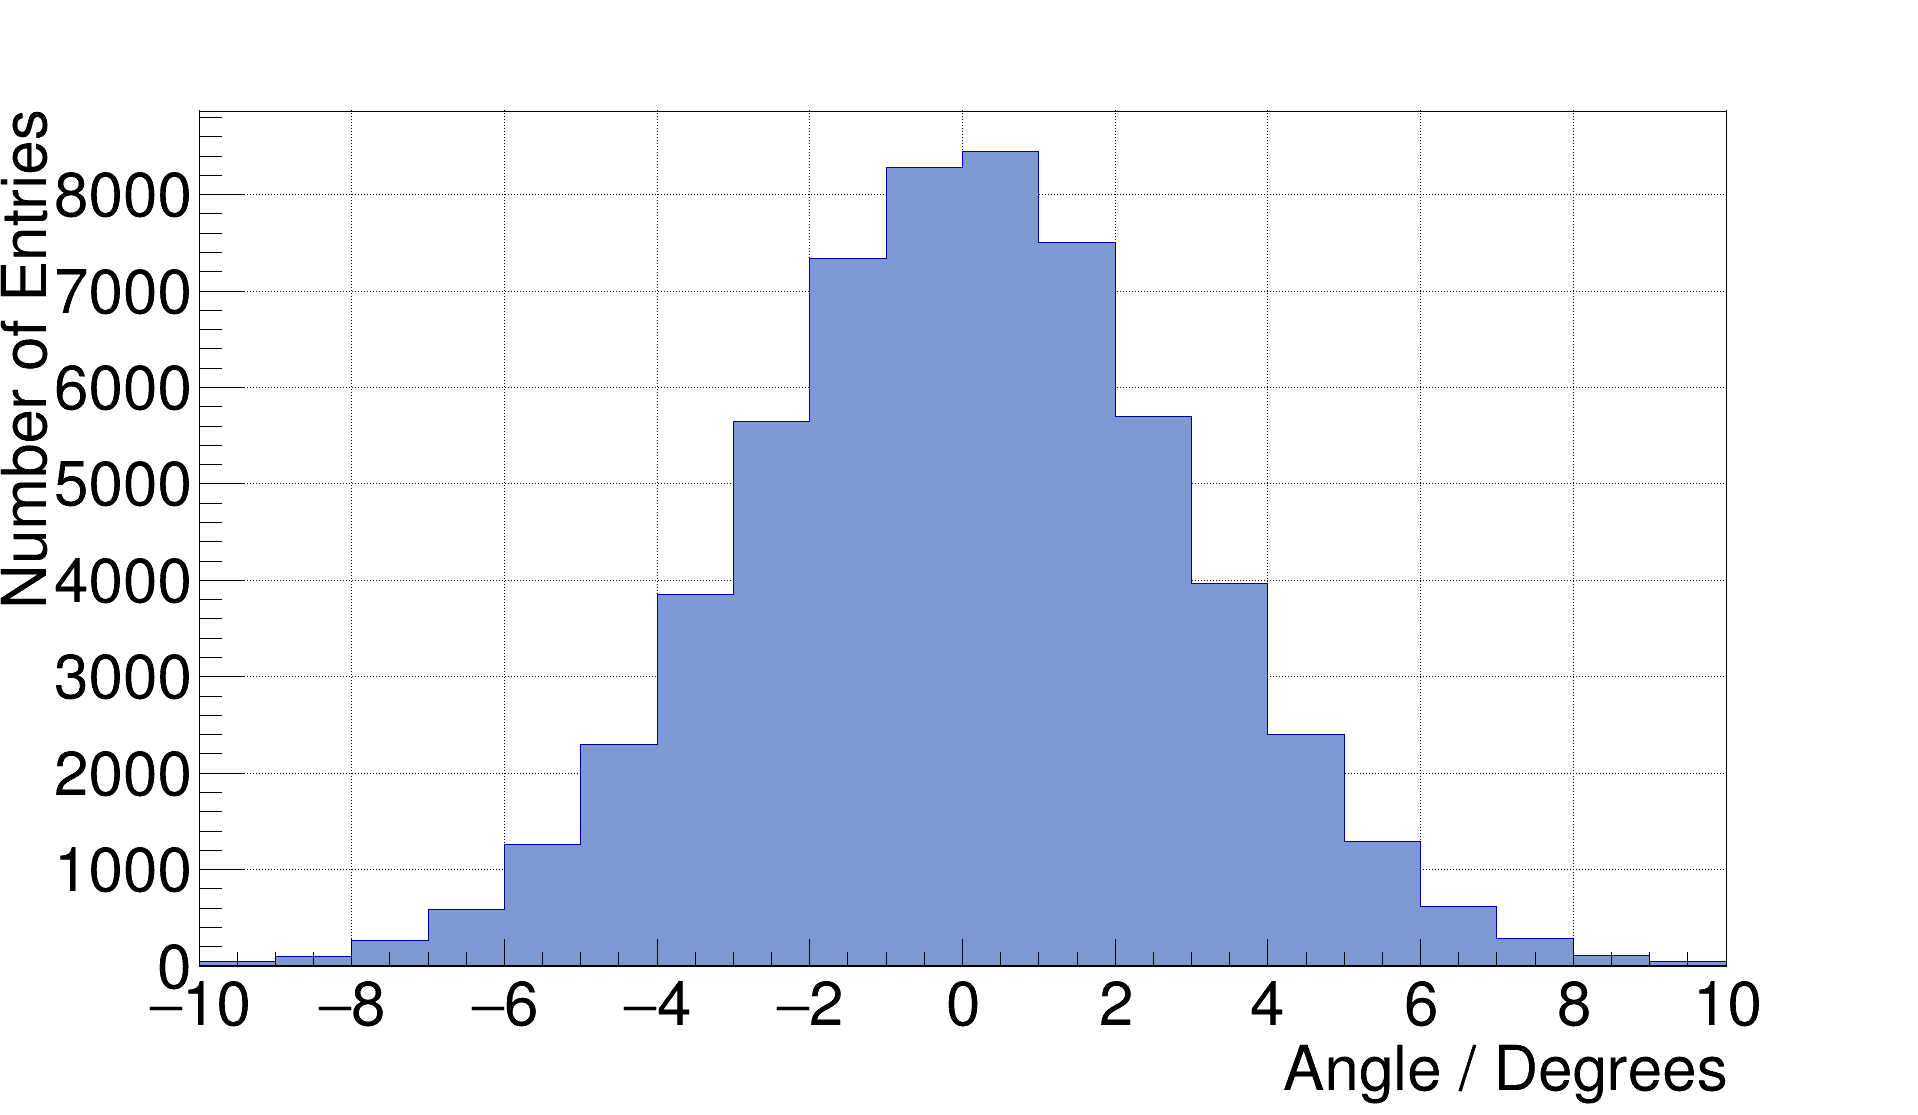
\includegraphics[width=74mm]{OeffZVertex/20170205DiffOeffZVertexUrsprung135MeV}
	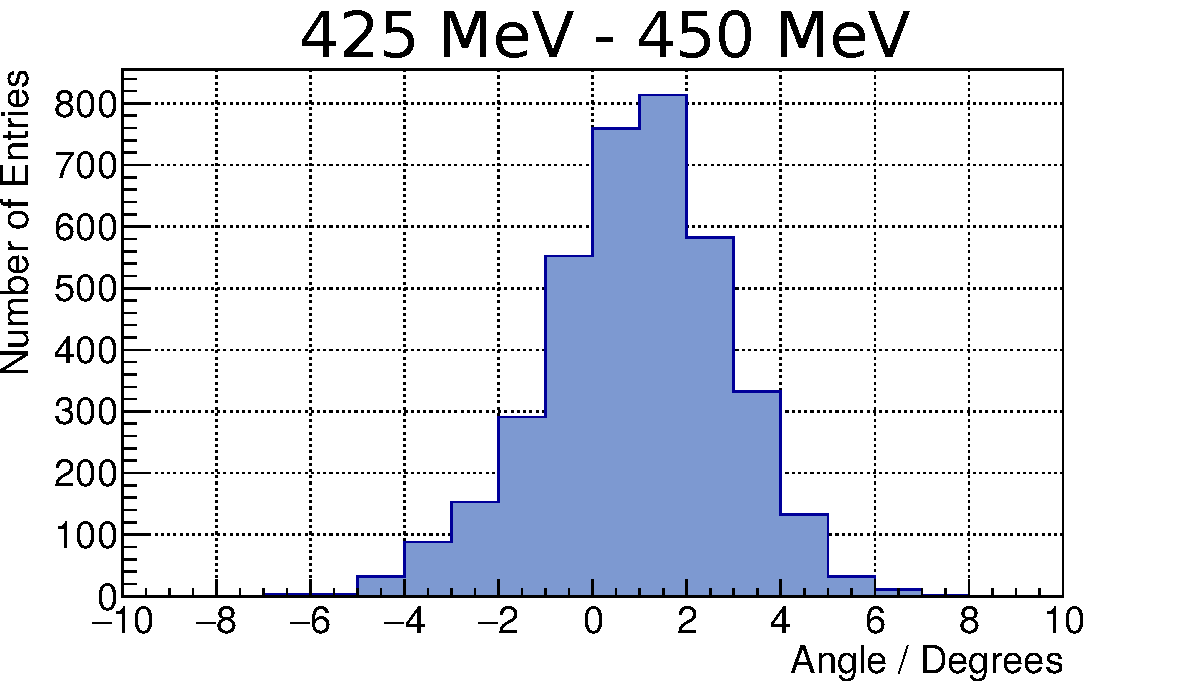
\includegraphics[width=74mm]{OeffZVertex/20170205DiffOeffZVertexUrsprung425MeV}
	\end{array}$
\end{center}


\begin{center}
	\text{Ende des Targets:}
	$
	\begin{array}{cc}
	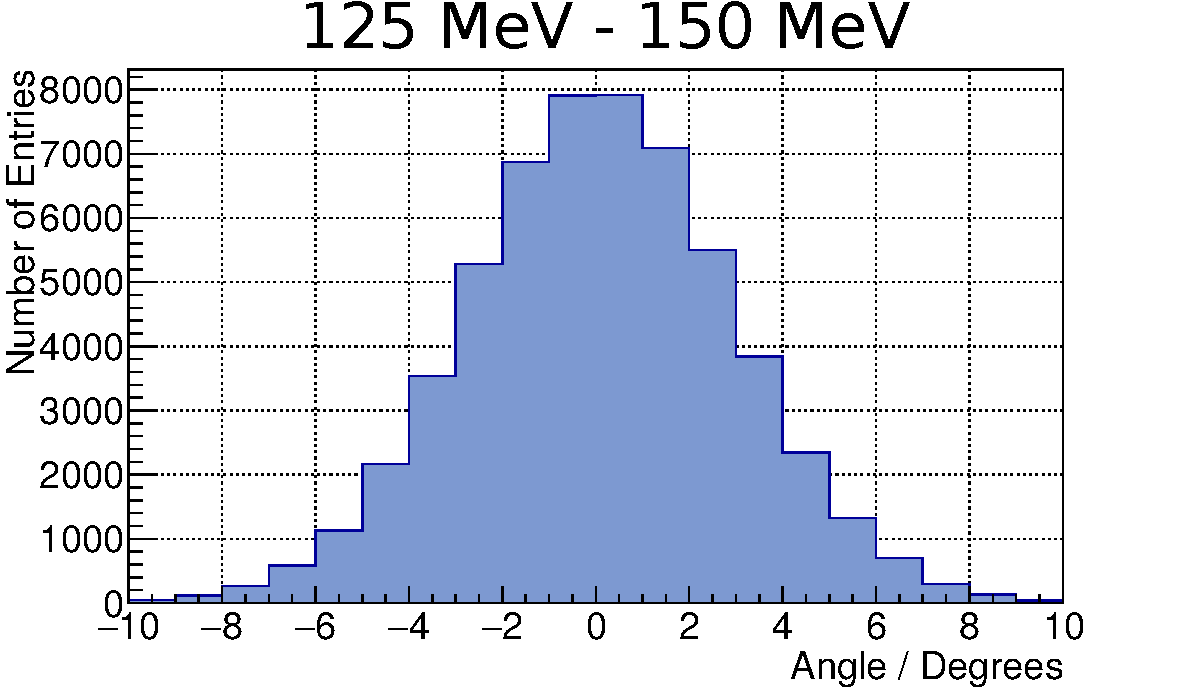
\includegraphics[width=74mm]{OeffZVertex/2017205DiffOeffZVertex+4_125MeV}
	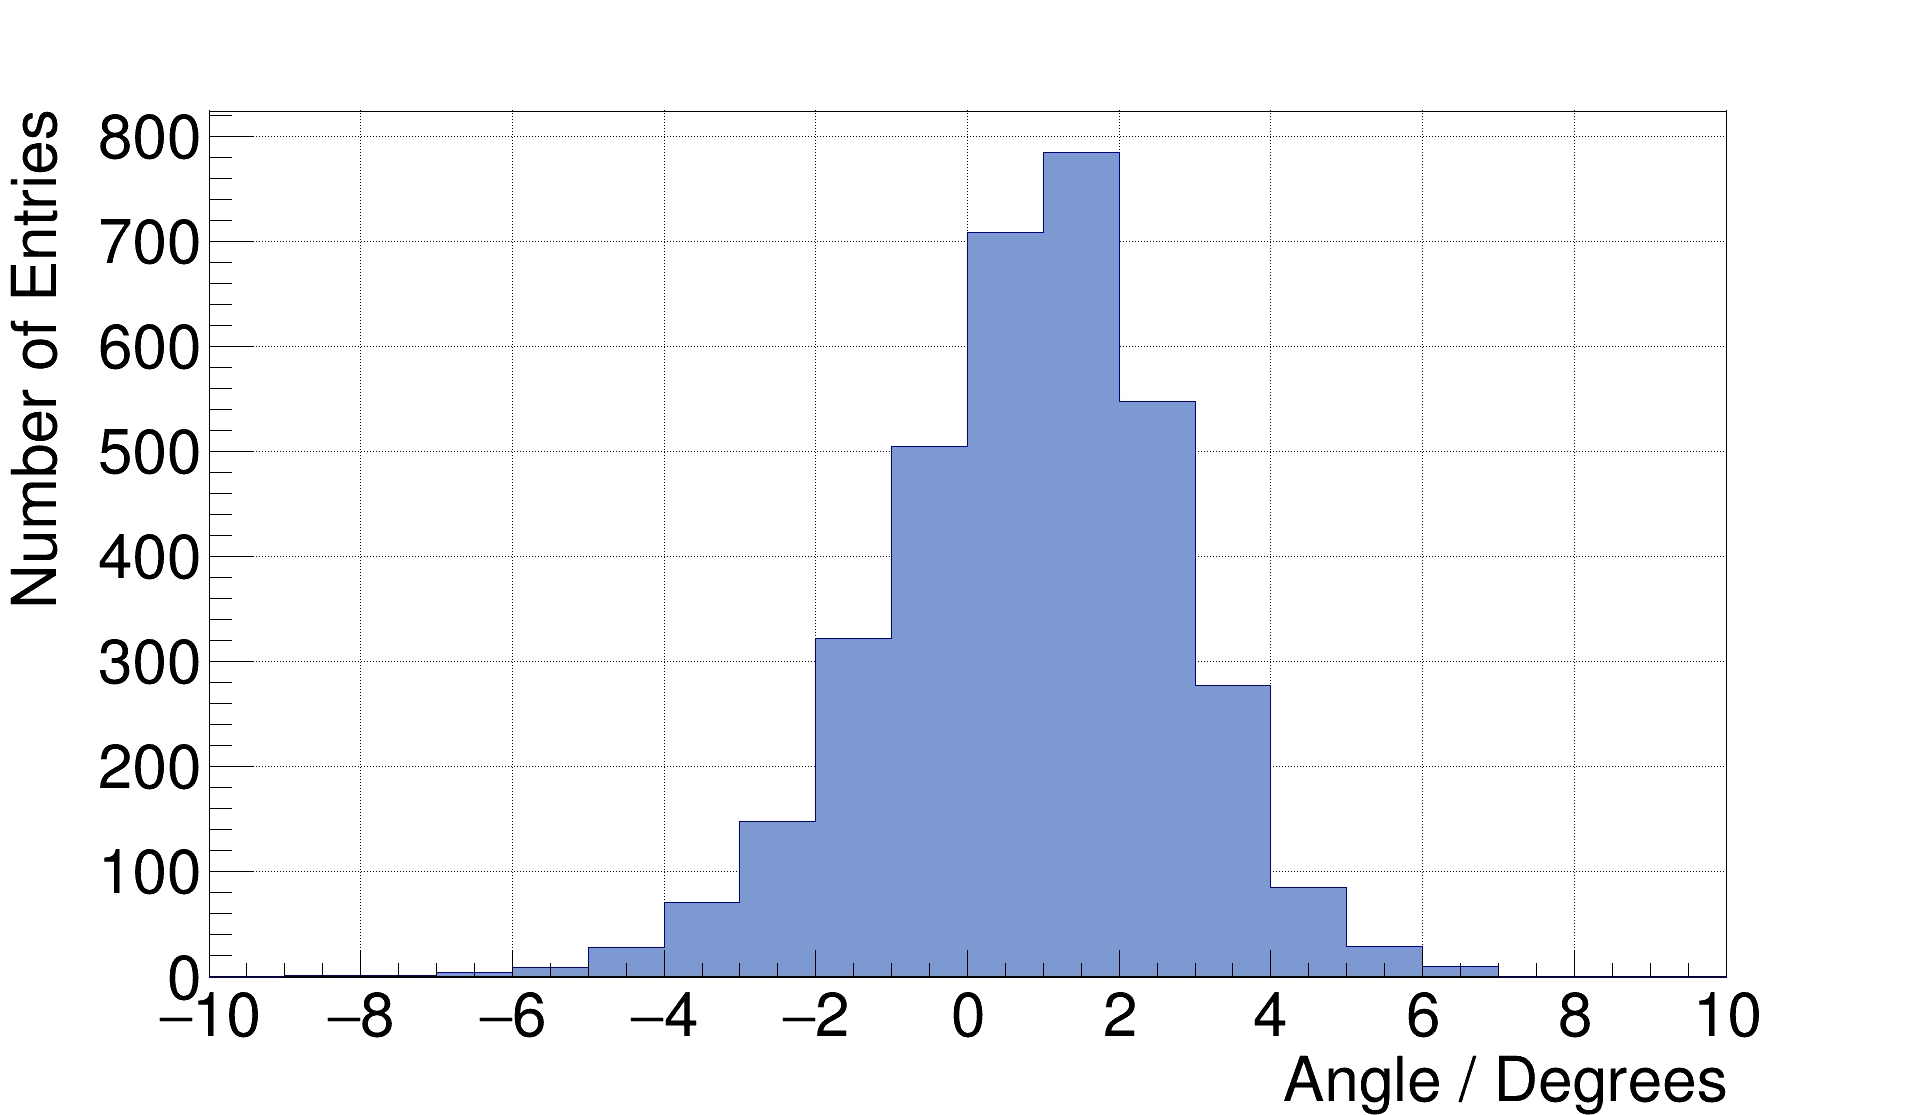
\includegraphics[width=74mm]{OeffZVertex/20170205DiffOeffZVertex+4_425MeV}
	\end{array}$
\end{center}

\caption[Simulation: Differenz zwischen gen. und kon. \"Offnungswinkel f\"ur verschiedene $z$-Vertices]{Daten aus der Simulation: Aufgetragen ist $\Delta \alpha$ f\"ur verschiedene $z$-Vertices und Energien. Die vollst\"andigen 2D-Histogramme sind in den Abbildungen \ref{fig:OeffZVertex-4} bis \ref{fig:OeffZVertex4} zu sehen.}
\label{fig:Oeffnungwinkel-Z-Vertex}
\end{figure}

In Abbildung \ref{fig:Oeffnungwinkel-Z-Vertex} sind die verschiedenen Abweichungen zwischen dem rekonstruierten und generierten \"Offnungswinkel f\"ur diese drei $z$-Vertex Intervalle abgebildet.

Hier erkennt man, dass es fast keinen Unterschied macht, wo im Target das $\pi^0$ zerf\"allt. Die Differenzen zwischen rekonstriurten und generierten Abweichungen sind f\"ur alle $z$-Vertices sehr \"ahnlich. Besonders f\"ur kleine Energien, in den Abbildungen immer links zu sehen, hier ist liegt die Photonenenergie zwischen $125\,\text{MeV}$ und $150\,\text{MeV}$, ist fast kein Unterschied zu erkennen. F\"ur Photonenenergien im Bereich von $425\,\text{MeV}$ bis $450\,\text{MeV}$, immer rechts abgebildet, ist eine sehr leichte Verschiebung nach rechts zu erkennen, wenn man sich vom Anfang des Targets zum Ende bewegt. Das hei{\ss}t, der rekonstruierte \"Offnugnswinkel ist gr\"o{\ss}er, wenn das $\pi^0$ am Ende des Targets zerfallen ist, im Vergleich zu einem Zerfall am Anfang des Targets. Allerdings ist dieser Effekt auch nur sehr klein und erkl\"art die Auff\"acherung, welche bereits in Abbildung \ref{fig:Z-Vertex-Multi-Graph} zu sehen war.


%Direkter Vergleich
\begin{comment}
\subsection{Direkter Vergleich zwischen der Energie der generierten und detektierten Photonen}
\label{sec-Vergleich-Energie-gen-rec}
 
 Da mit den Betrachtungen keine Ursache f\"ur die starke Abweichung gefunden werden konnte, wurde auch einmal die Energie der detektierten Teilchen mit der tats\"achlichen Energie verglichen. Diese Betrachtung geschah aus reinem Interesse, da mit diesem Ergebnis nicht auf eine Abweichung vom $\pi^0$-Peak geschlussfolgert werden konnte. 
 
 Das lag daran, dass der Detektor auf den $\pi^0$-Peak kalibriert wird und nicht auf die detektierten Energien, weil die detektierte Energie nie der tats\"achlichen Energie entspricht. 

 
\begin{figure}[h!]
	\begin{center}$
		\begin{array}{c}
		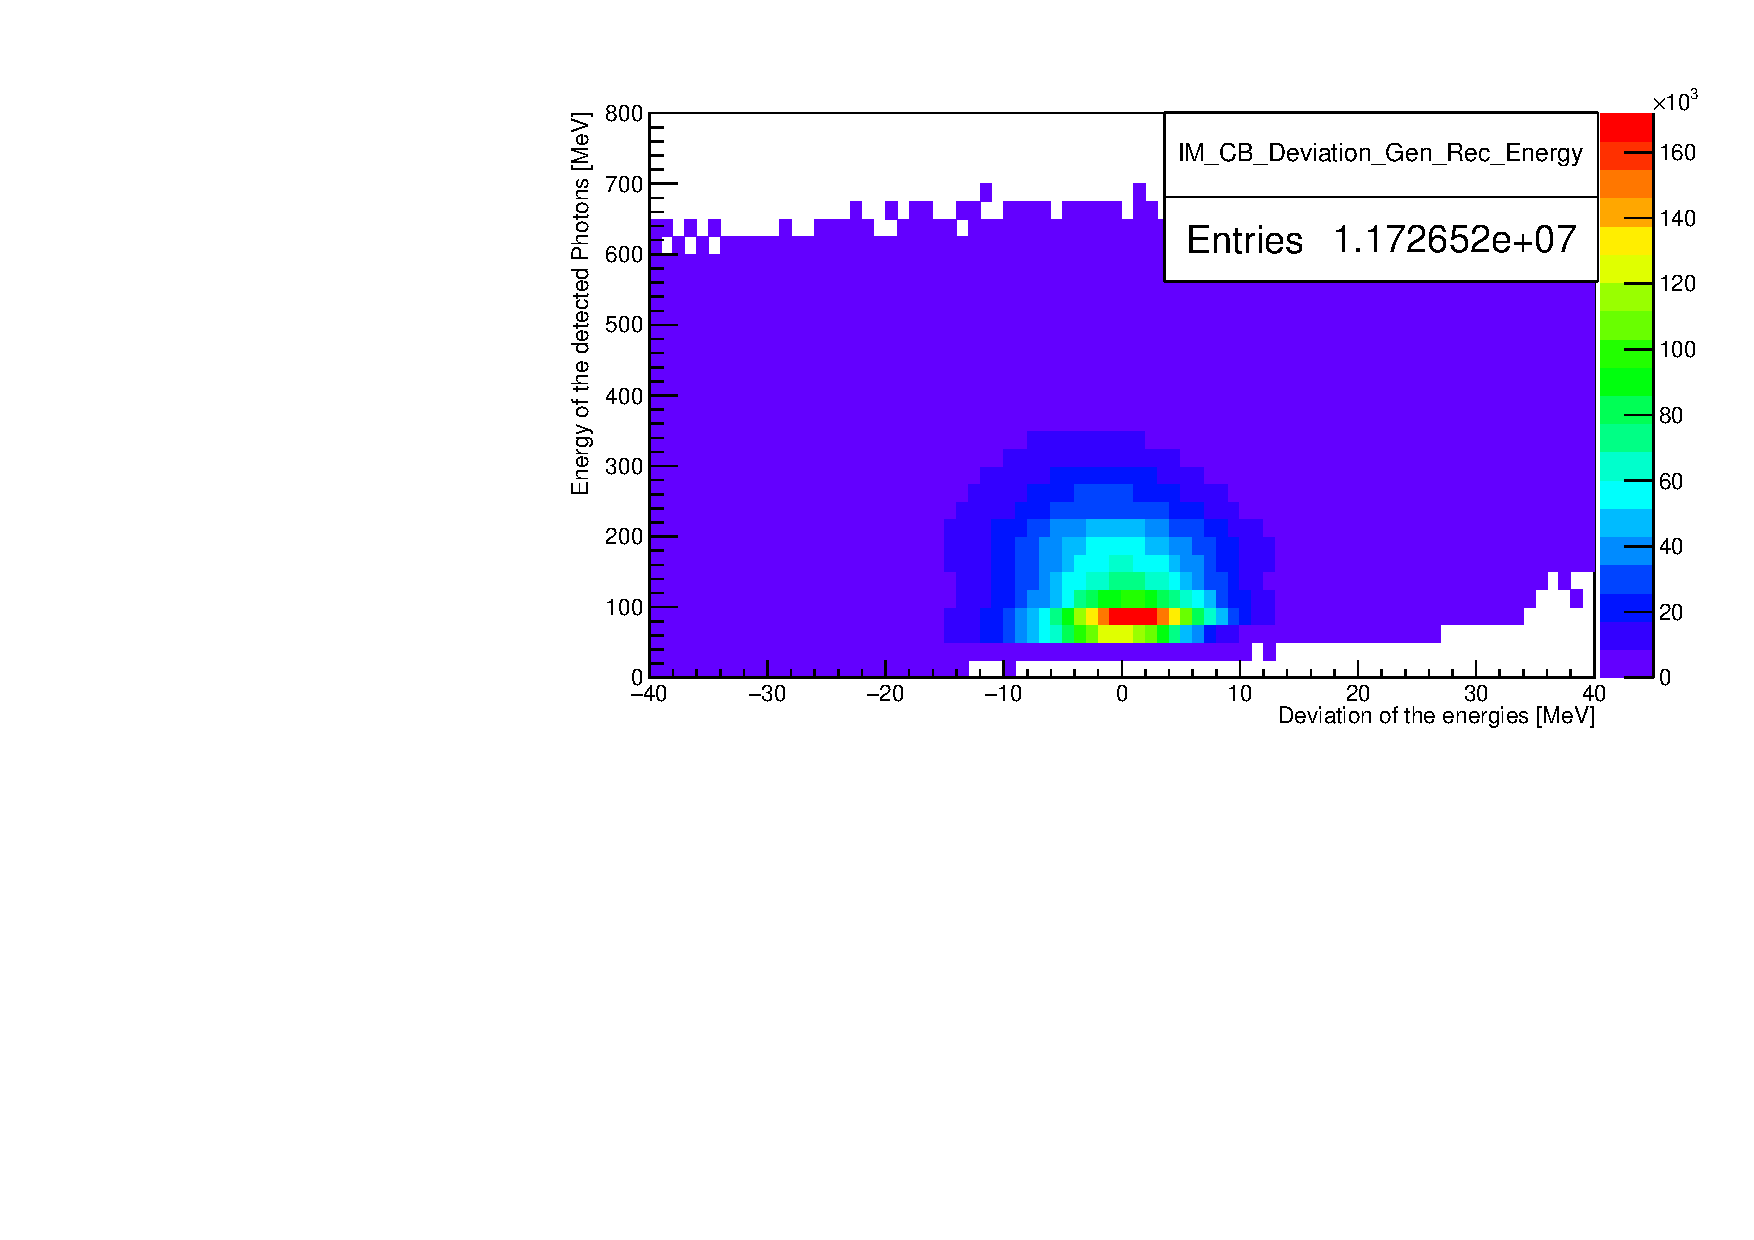
\includegraphics[width=100mm]{NewCalib/20171904SimErec-EgenDeviation}
		\end{array}$
	\end{center}

	\begin{center}$
		\begin{array}{cc}
			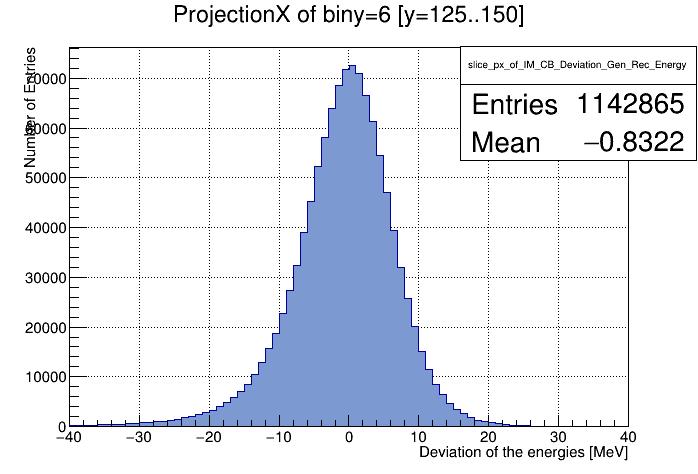
\includegraphics[width=75mm]{NewCalib/20171904SimErec-EgenDeviation125MeV}
			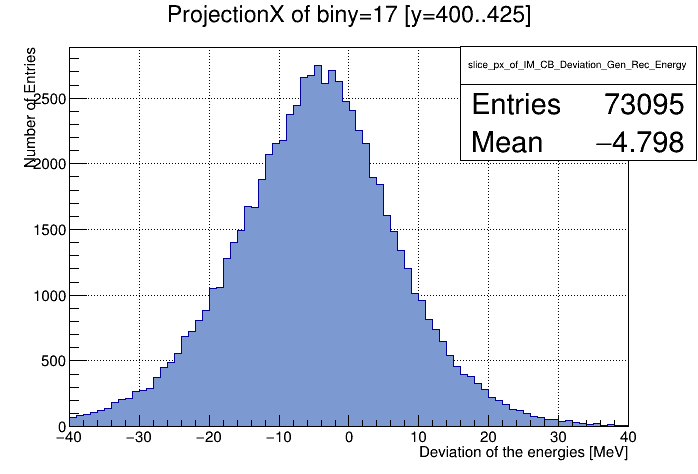
\includegraphics[width=75mm]{NewCalib/20171904SimErec-EgenDeviation400MeV}
		\end{array}$
	\end{center}
\caption{Von der im Detektor gemessenen Energie wurde die tats\"achliche Energie der Teilchen abgezogen. Oben ist dies f\"ur verschiedene Photonenenergien dargestellt. Unten sind zwei Energieintervalle als Beispiel herausgenommen. Links besa{\ss}en die detektierten Photonen eine Energie von 125 MeV bis 150 MeV, rechts von 400 MeV bis 425 MeV.}
\label{fig:Erec-Egen}
\end{figure}
 

 In den Plots von Abbildung \ref{fig:Erec-Egen} wurde die tats\"achliche Energie der Teilchen von der detektierten abgezogen. Sprich liegt eine positive Abweichung vor, dann wurde zu viel Energie im Detektor registriert und vise versa.
 
 Zu sehen ist hier allerdings, dass die im Detektor registrierte Energie in der Regel kleiner war, als die tats\"achliche Energie der Teilchen.
 Also selbst wenn man aus dem direkten Vergleich zwischen detektierter Energie und tats\"achlicher Energie einen Schluss ziehen k\"onnte, k\"onnte man damit nicht erkl\"aren, warum f\"ur hohe Photonenenergien eine zu gro{\ss}e $\pi^0$ Masse berechnet wird, da die gemessene Energie sogar kleiner als die tats\"achliche ist.
\end{comment}

\chapter{Weitere Beobachtungen}
\label{sec:Weitere-Beobachtungen}

Auch hier werden nur Photonen mit einer \"ahnlichen Energie betrachtet. $|E_{\gamma_1}-E_{\gamma_2}|<25\,\text{MeV}$


\section{Defekte und rauschende Kristalle}


\subsection{Verhalten von bereits bekannten defekten und rauschenden Kristallen}
\label{sec:Bekannte-Dead-Crystals}
Ein rauschender Kristall ist ein Detektorkristall, der Events registriert, obwohl es kein einfallendes Teilchen gibt. Durch diese St\"orung der Detektoren, k\"onnen also Teilchen falsch zugeordnet werden, was zu einer falschen berechneten invarianten Masse f\"uhrt. 

Ein defekter Kristall auf der anderen Seite ist ein Kristall, welcher nicht mehr funktioniert und kein Signal mehr von sich gibt.

Betrachtet man Abbildung \ref{fig:Verteilung-im-CB} links, so entsteht bereits hier die Vermutung, dass es mindestens einen rauschenden Kristall im Crystal-Ball Detektor gibt. Der beste Kandidat ist bei einem Azimutwinkel von 160$^{\circ}$ und einem Polarwinkel von 95$^{\circ}$ zu finden.

Um nun mehrere dieser rauschenden Kristalle zu finden, wird Abbildung \ref{fig:Verteilung-im-CB} noch einmal mit einer anderen Photonenenergie dargestellt. Auch werden nur Photonen eingetragen, deren berechnete invariante Masse in einem Bereich von $70\,\text{MeV}$ bis $220\, \text{MeV}$ liegen. Es werden die Daten aus der Strahlzeit genommen.

\begin{figure}[h!]
	\begin{center}
		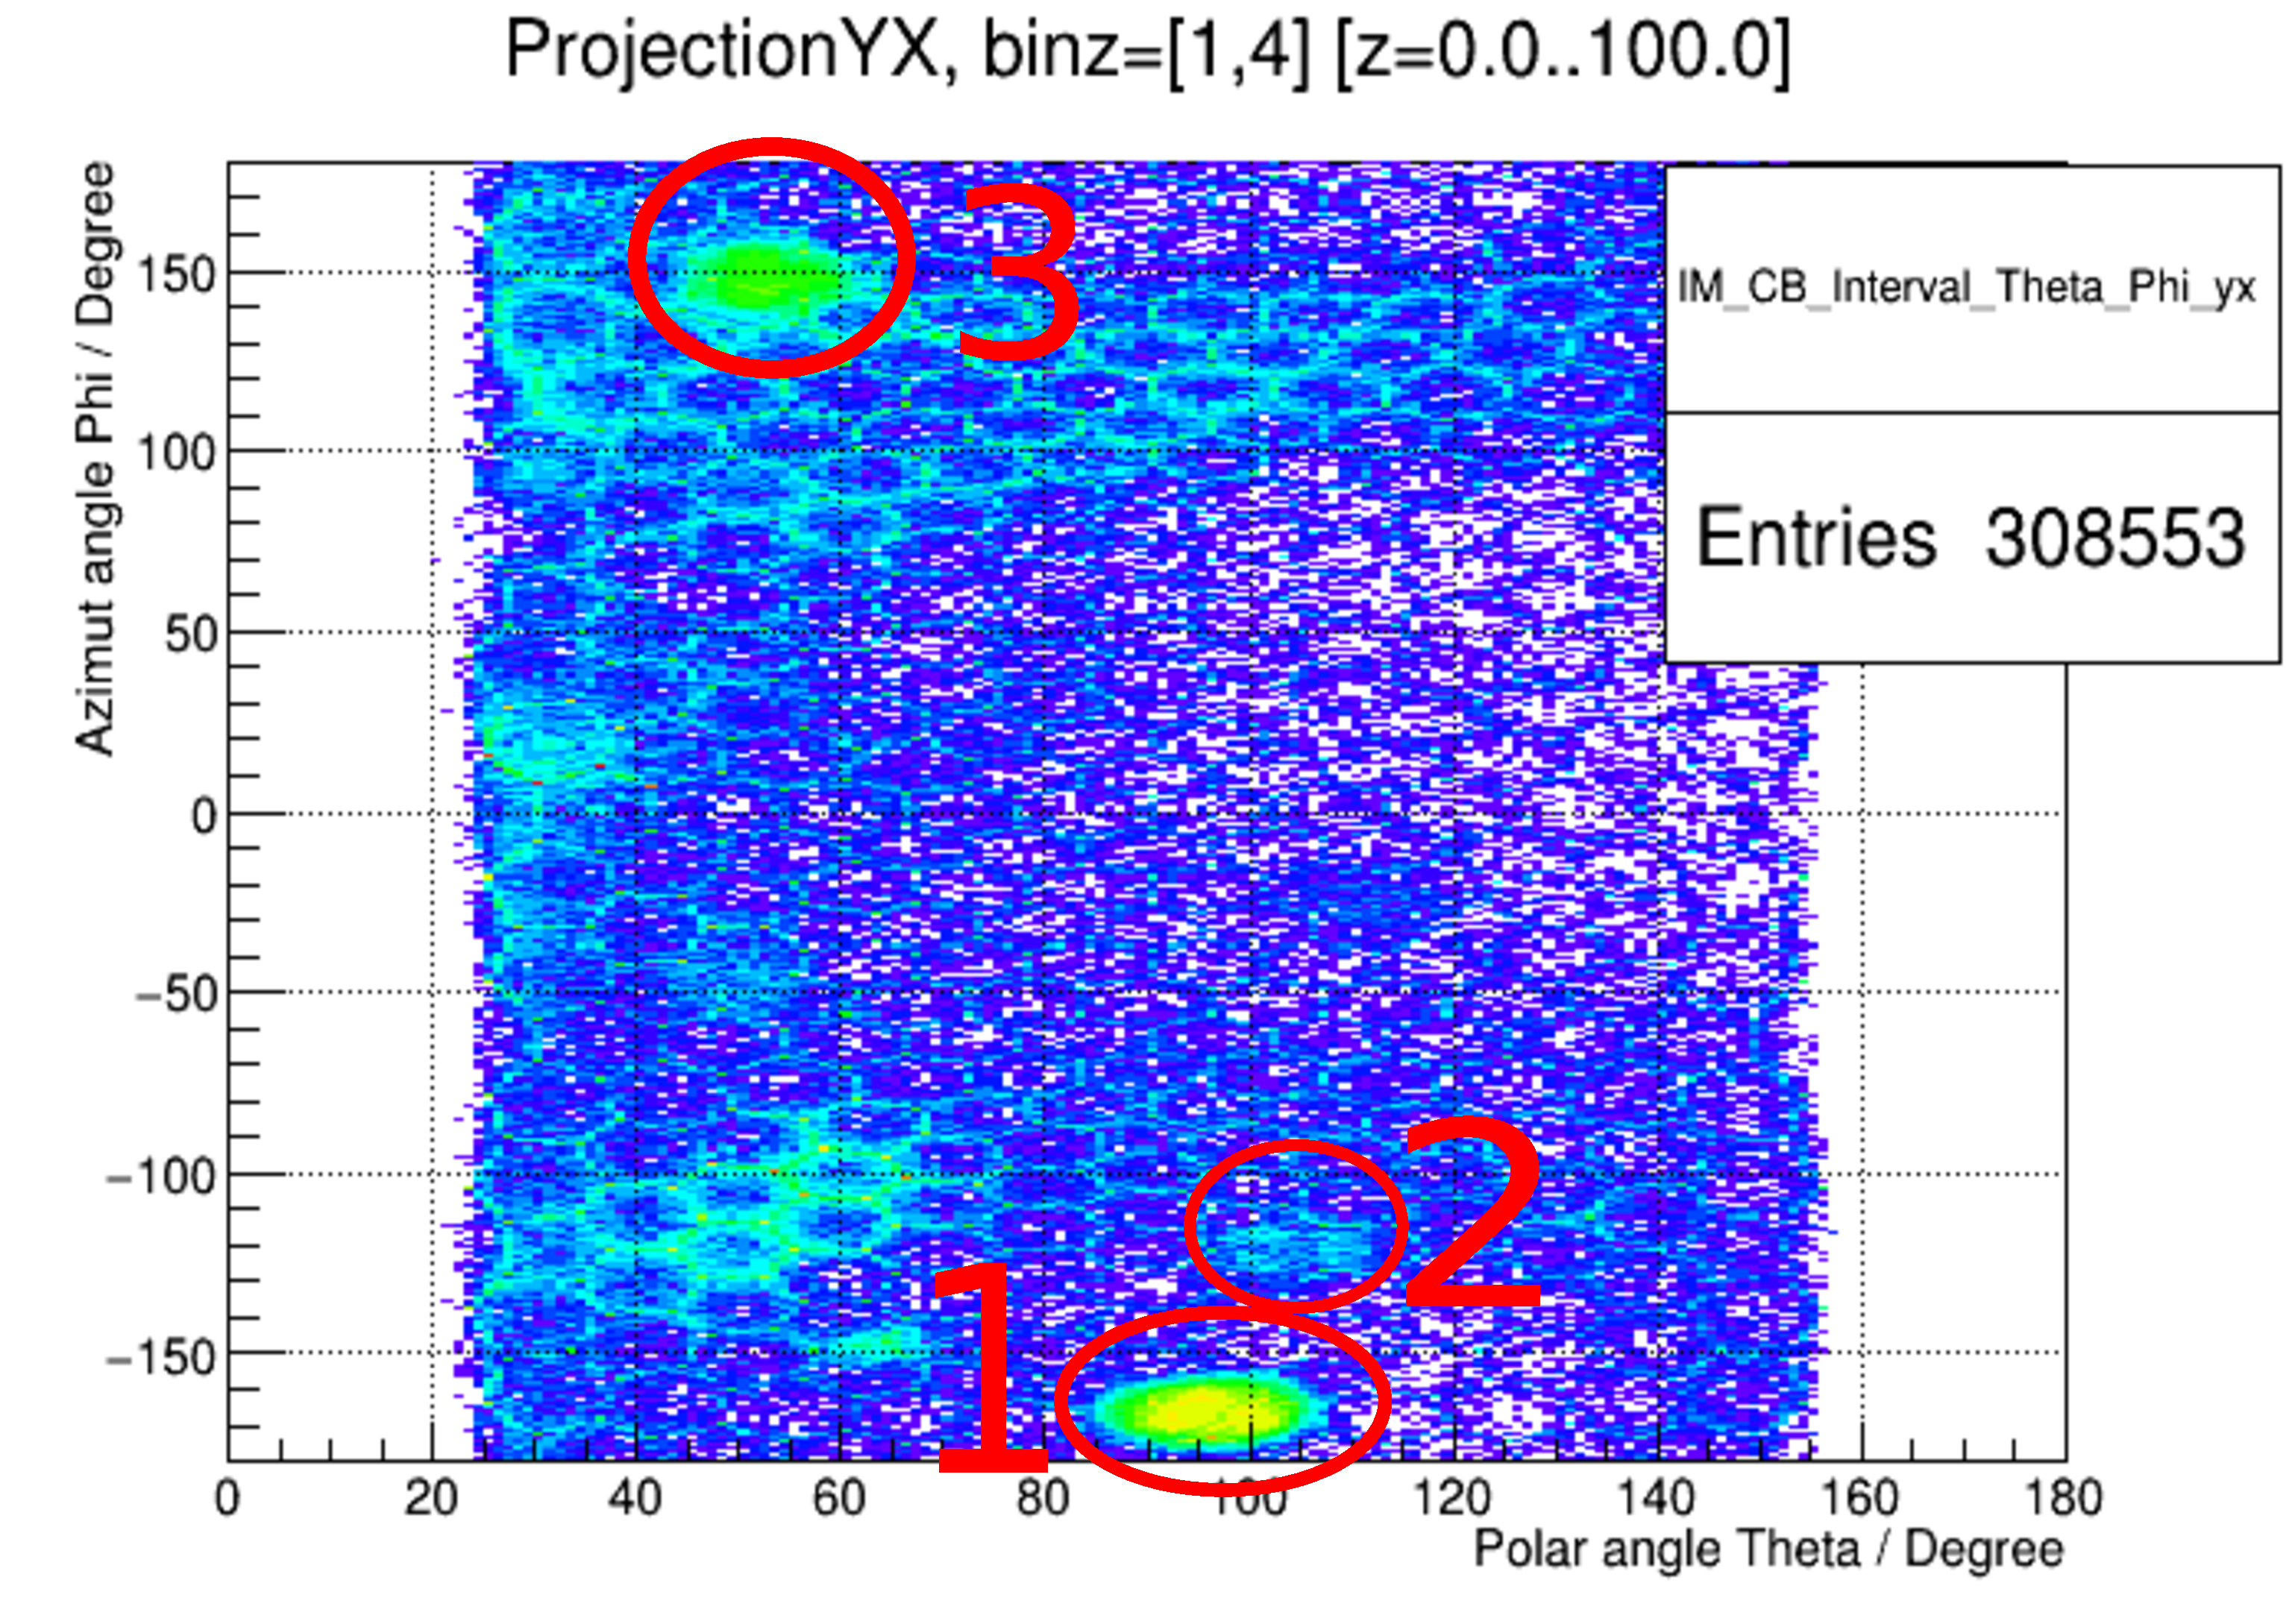
\includegraphics[width=100mm]{NewCalib/Strahlzeit2014/ClusterSize/20172104StrahlzeitClusterSize0Marker}
	\end{center}
	\caption[Strahlzeit: Markierte rauschende Kristalle; Niedrige Energien]{Daten aus der Strahlzeit: Verteilung der detektierten Teilchen im Crystal-Ball. Die Energie der Teilchen muss \"ahnlich sein und liegt im Intervall von $0\,\text{MeV}$ bis $100\,\text{MeV}$. Markiert sind m\"ogliche rauschende Kristalle}
	\label{fig:Markierte-Hot-Crystals}
\end{figure}

In Abbildung \ref{fig:Markierte-Hot-Crystals} ist die Verteilung der registrierten Teilchen im Crystal-Ball f\"ur eine Photonenenergie von $0\,\text{MeV}$ bis $100\,\text{MeV}$ dargestellt. Hier wurden 3 m\"ogliche Kandidaten f\"ur rauschende Kristalle mit roten Kreisen markiert. 


Um sich nun besser orientieren zu k\"onnen, wird mit den gleichen Daten eine Karte des Crystal-Balls gef\"ullt, auf der jeder Detektor dargestellt ist.
Anschlie{\ss}end wird versucht die Position der rauschenden Kristalle auch auf Crystal-Ball Karte zu finden und zuzuordnen.




\begin{figure}[h!]
	\begin{center}
		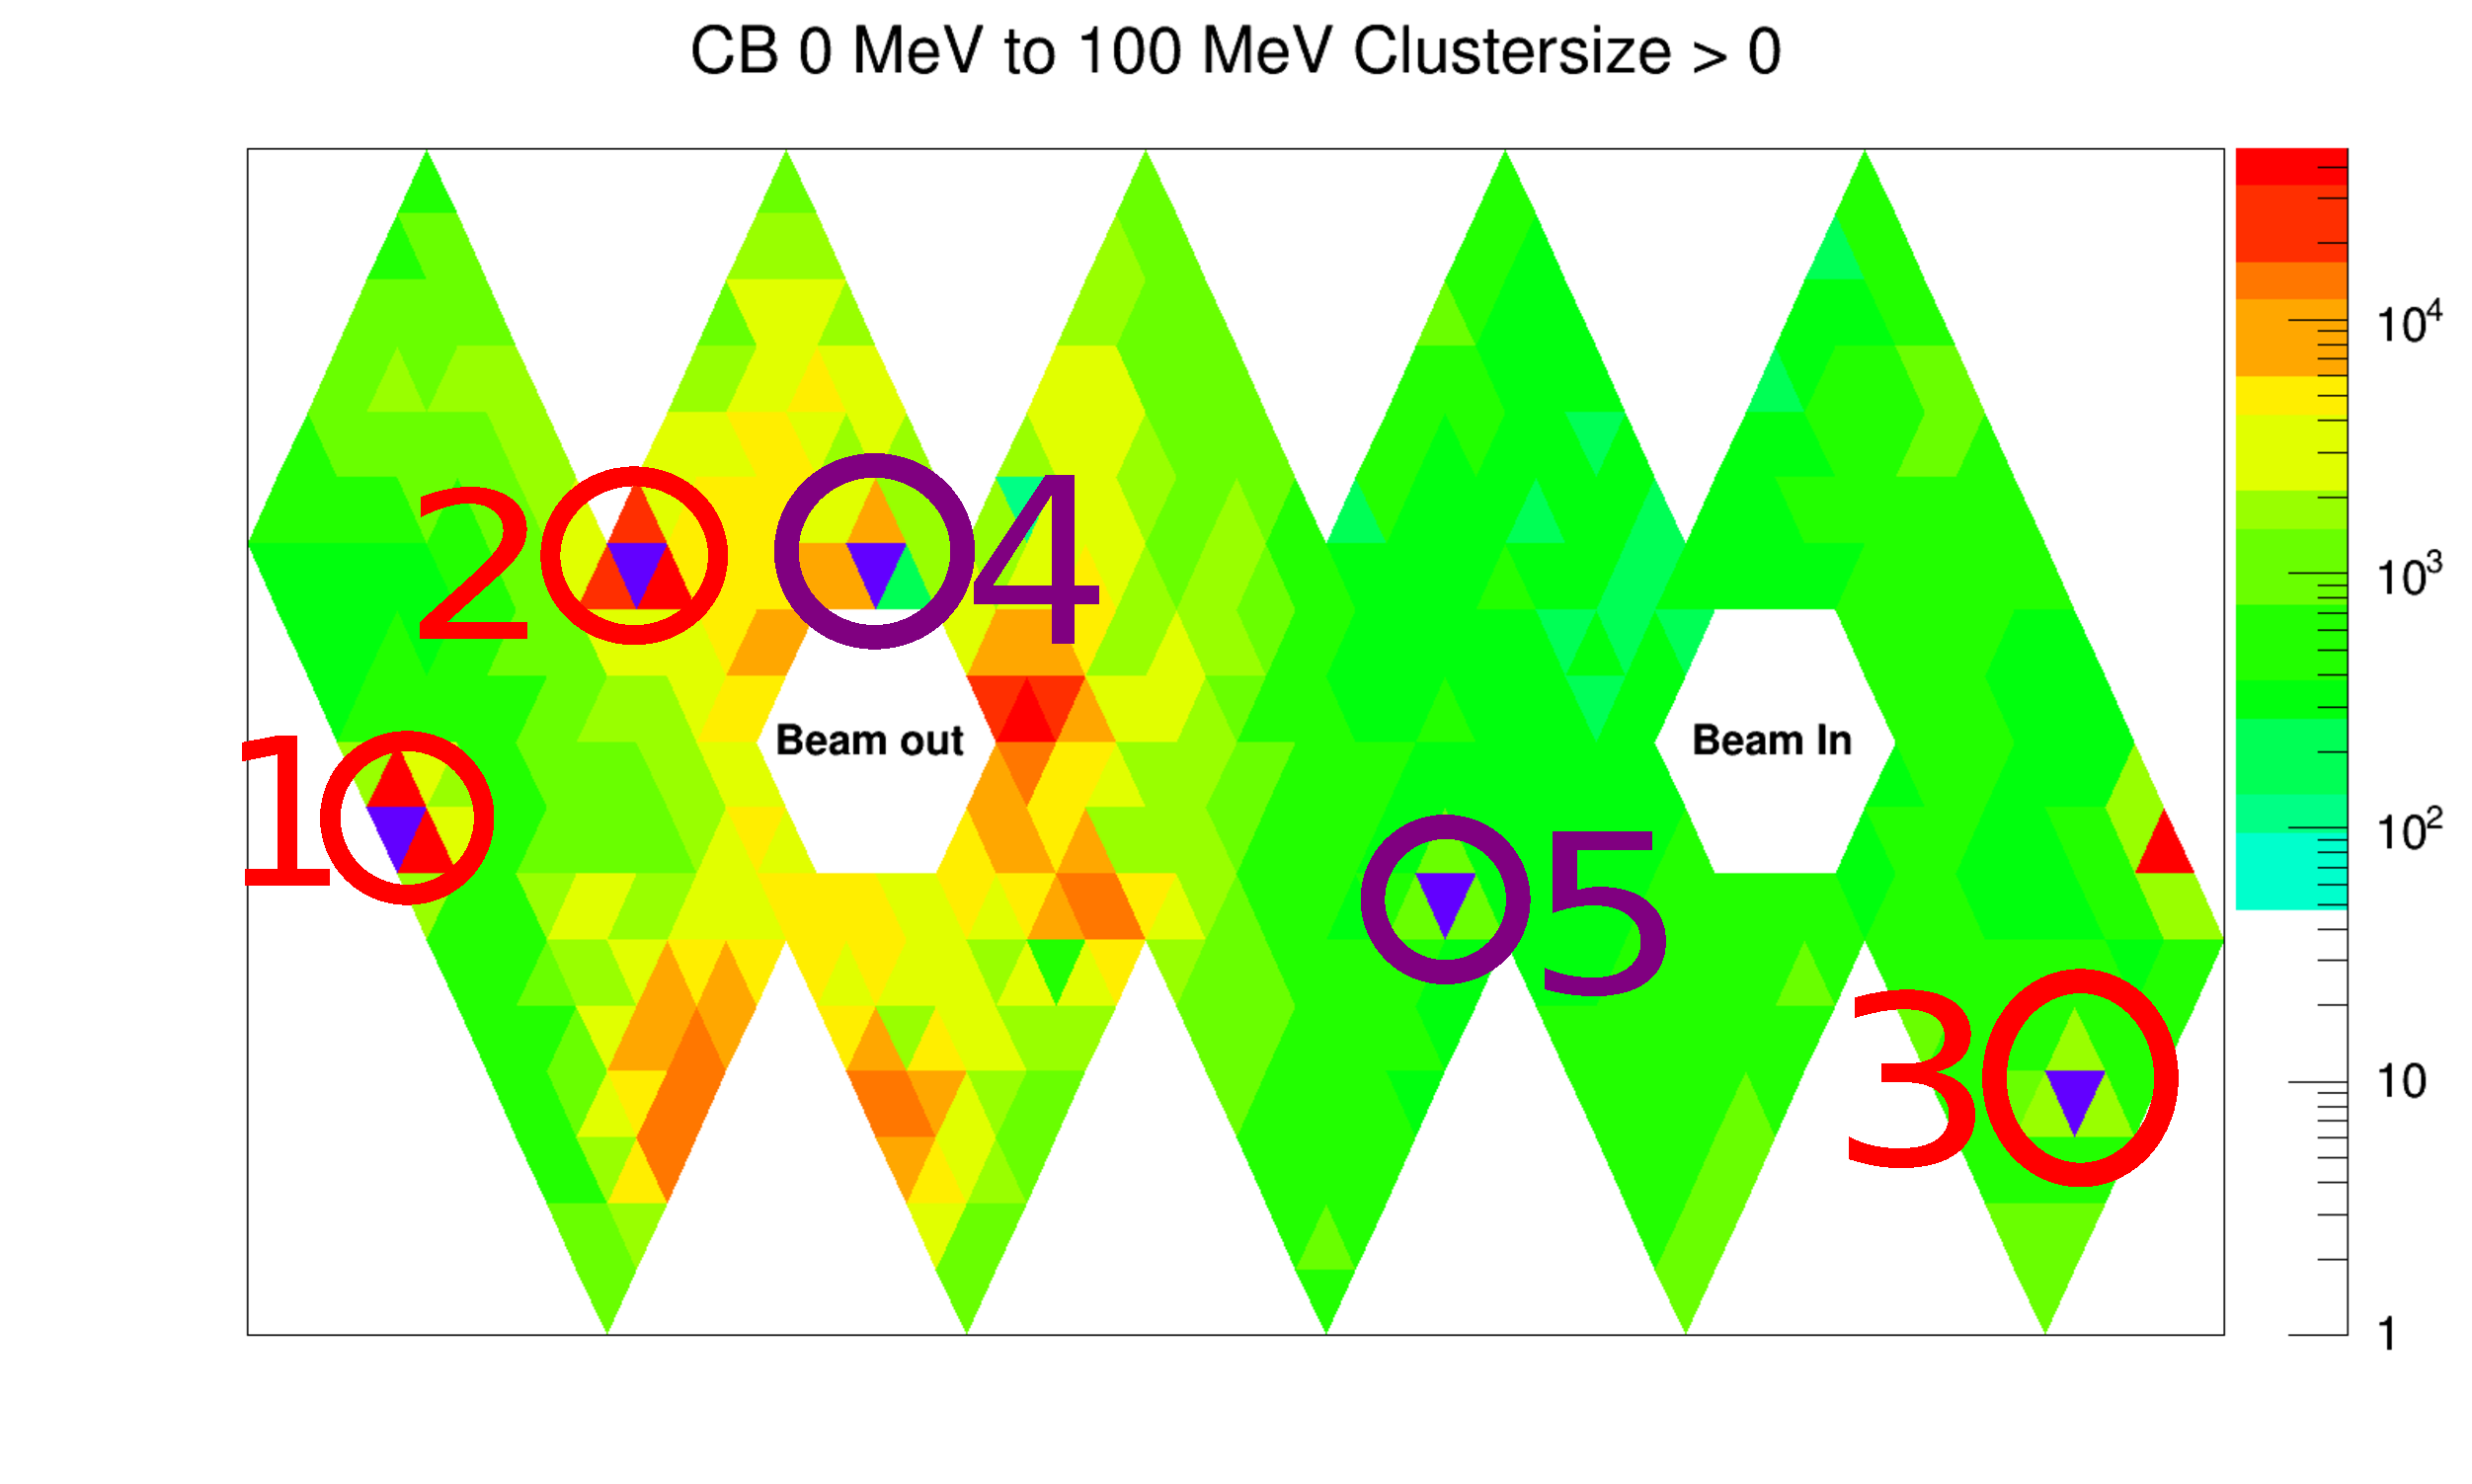
\includegraphics[width=100mm]{NewCalib/Strahlzeit2014/ClusterSizeNew/20172404Clustersize0Map100MeV}
		\caption[Strahlzeit: Markierte defekte Kristalle auf der CB-Karte; Niedrige Energien]{Daten aus der Strahlzeit: Crystal-Ball Map f\"ur eine Photonenenergie von $0\,\text{MeV}$ bis $100\,\text{MeV}$. Markiert sind die gleichen Kristalle, wie in Abbildung \ref{fig:Markierte-Hot-Crystals} und in lila zwei weitere tote Kristalle}
		\label{fig:Makierte-Kristalle-Map}
	\end{center}
\end{figure}

Wie in Abbildung \ref{fig:Makierte-Kristalle-Map} zu sehen ist, handelte es sich bei den vermuteten rauschenden Kristalle um defekte Kristalle. Diese sind allerdings von Kristallen umgeben, die deutlich mehr Events registriert haben als erwartet.

Die violett umkreisten Detektoren sind auch defekte Kristalle, diese verhalten sich allerdings anders, als die rot eingekreisten, da sie in Abbildung \ref{fig:Markierte-Hot-Crystals} nicht auffallen.

Mithilfe der Karte ist es auch m\"oglich die genaue Elementnummer der Kristalle zu bestimmen. Dies ist in Tabelle \ref{tab:Dead-Crystals} ist sehen. 

\begin{table}[h!]
	\centering
	
\begin{tabular}{lcc}

	Nummer in Abb. & Elementnummer&Anzahl der Events \\
	
	\hline
	1 & 549 &0 \\
	

	2 & 565& 0\\
	
	3 & 597 &0 \\
	
	4 & 677& 0\\
	
	5 & 265& 0\\
	
\end{tabular}
		

	\caption[Strahlzeit: Bereits bekannte defekte Kristalle]{Daten aus der Strahlzeit: Tabelle mit den bereits bekannten defekten Kristallen. An der Anzahl der Events erkennt man auch, dass die Detektoren ausgeschaltet sind.}
	\label{tab:Dead-Crystals}
\end{table}


\begin{figure}[h!]
\begin{center}$
	\begin{array}{cc}

		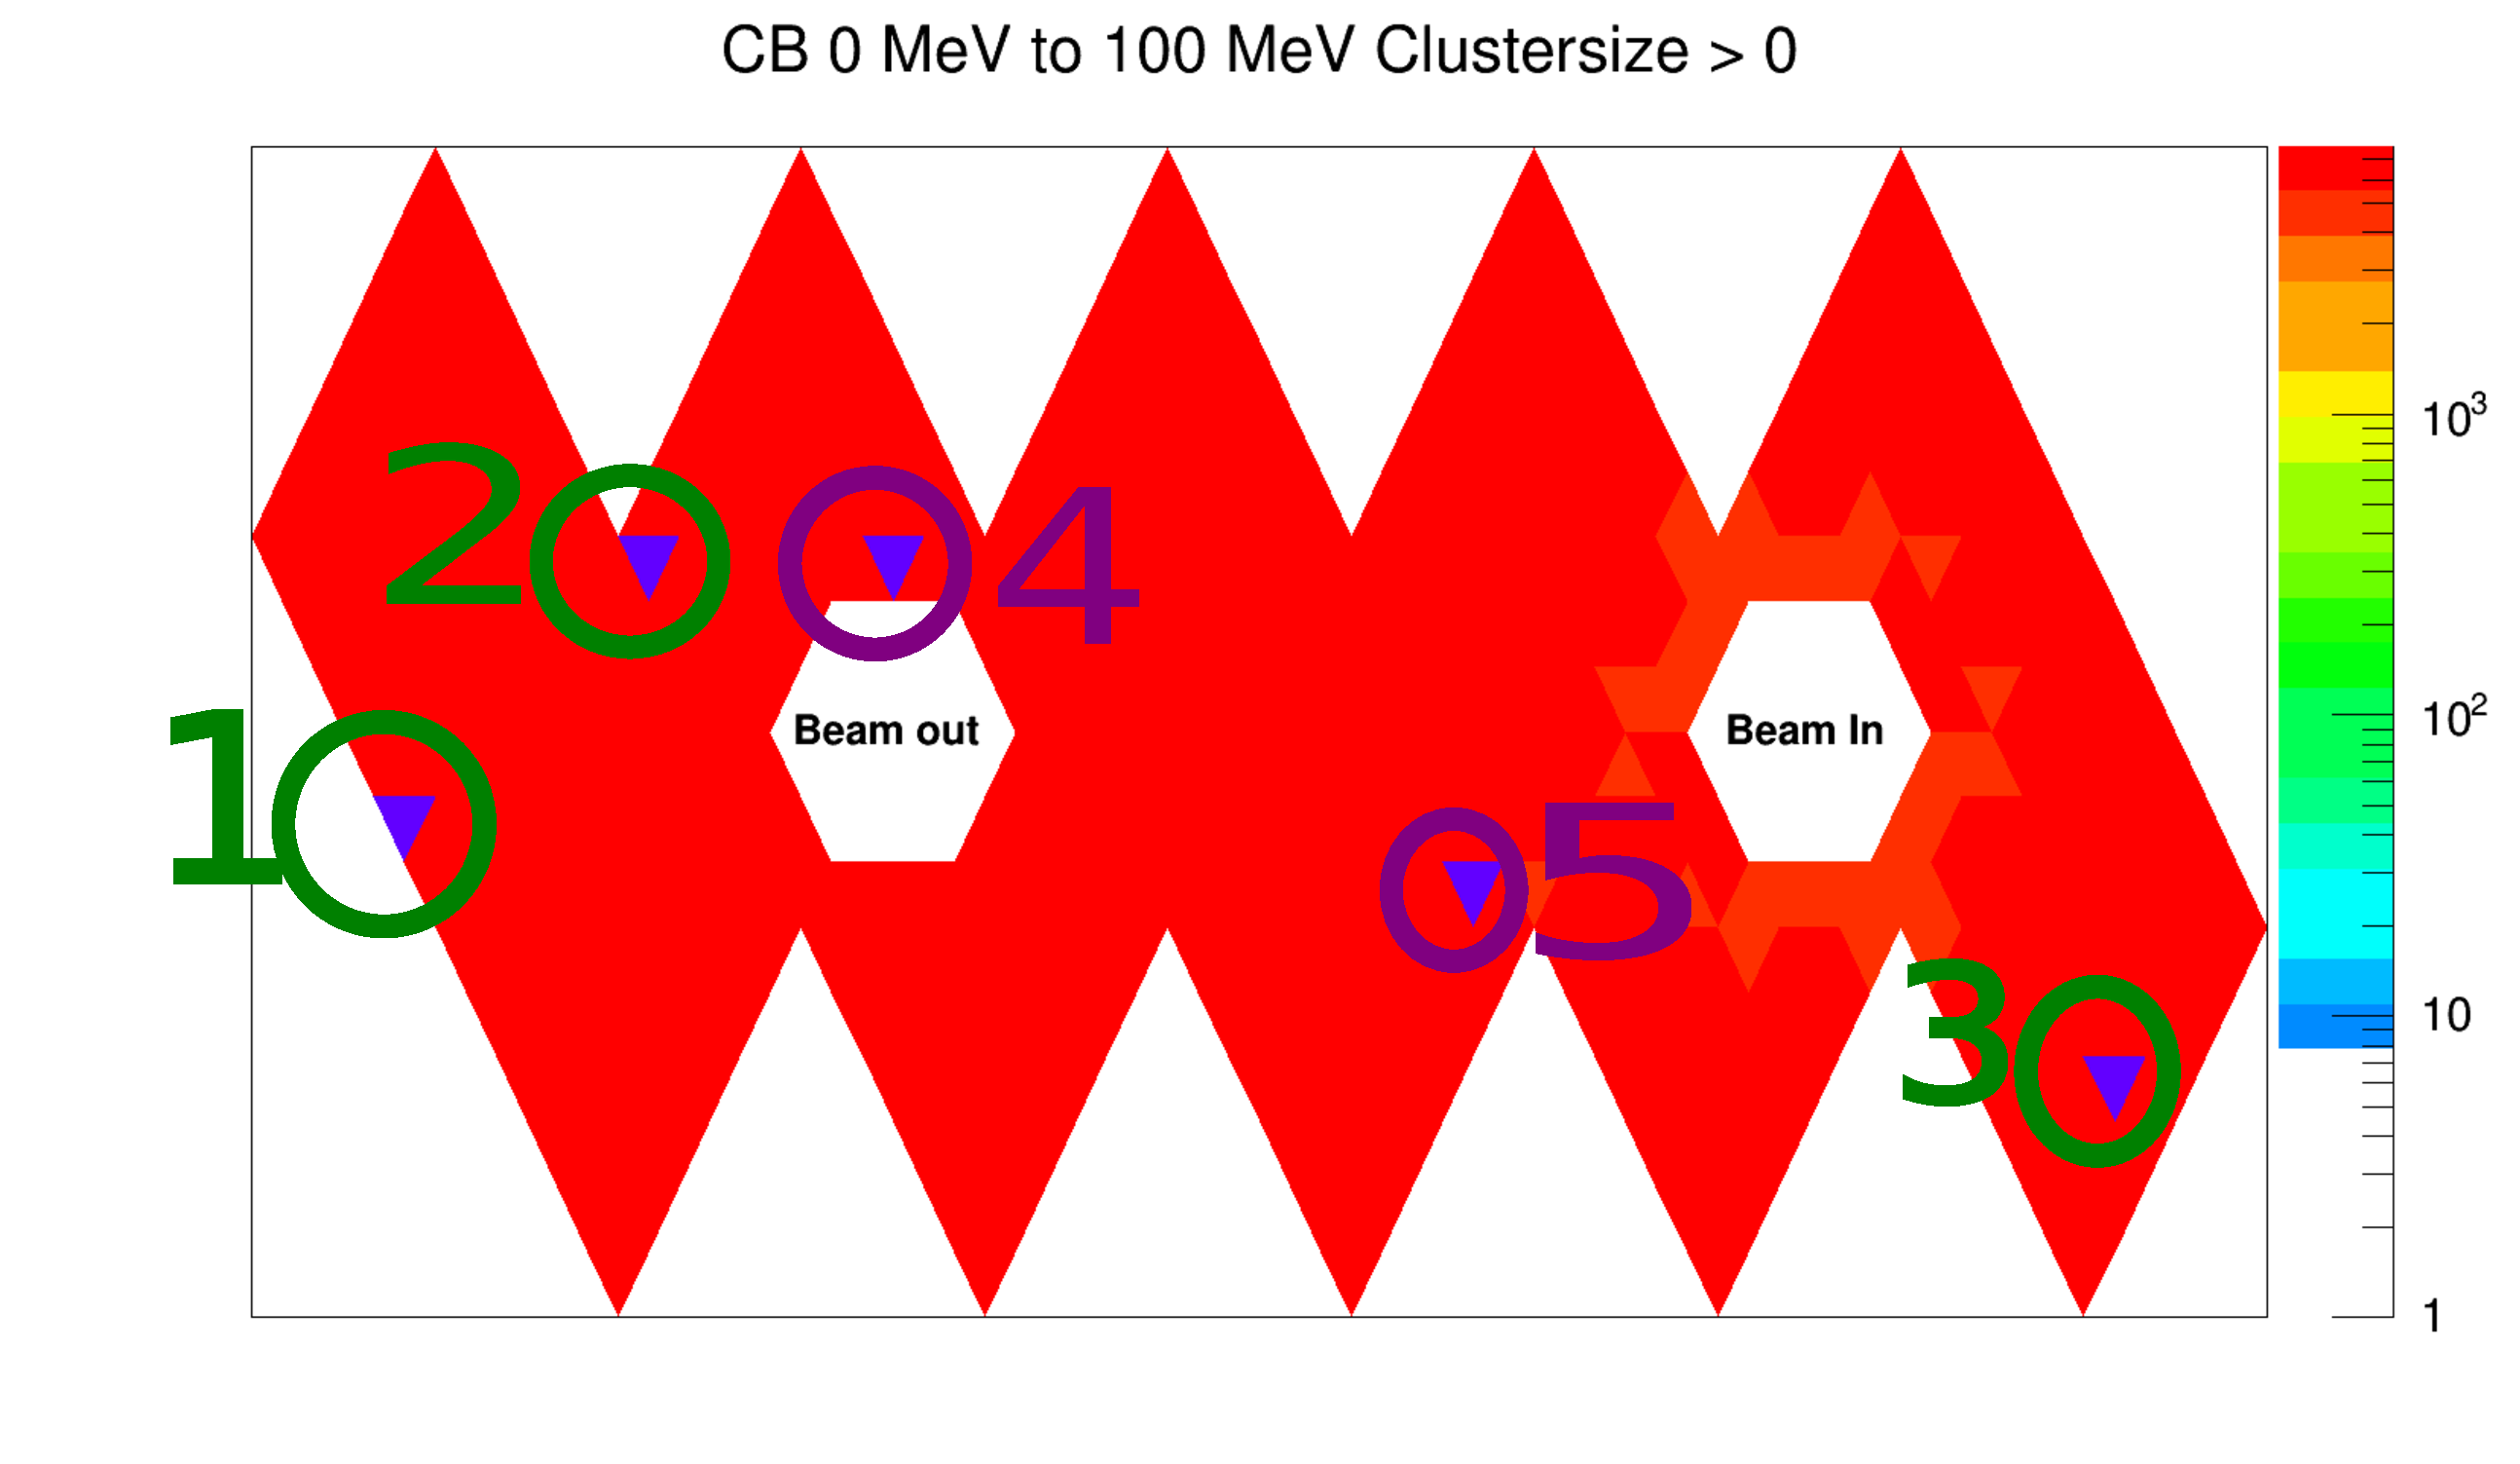
\includegraphics[width=74mm]{NewCalib/Strahlzeit2014/ClusterSizeNew/20172404MCClustersize0Map100MeV}

		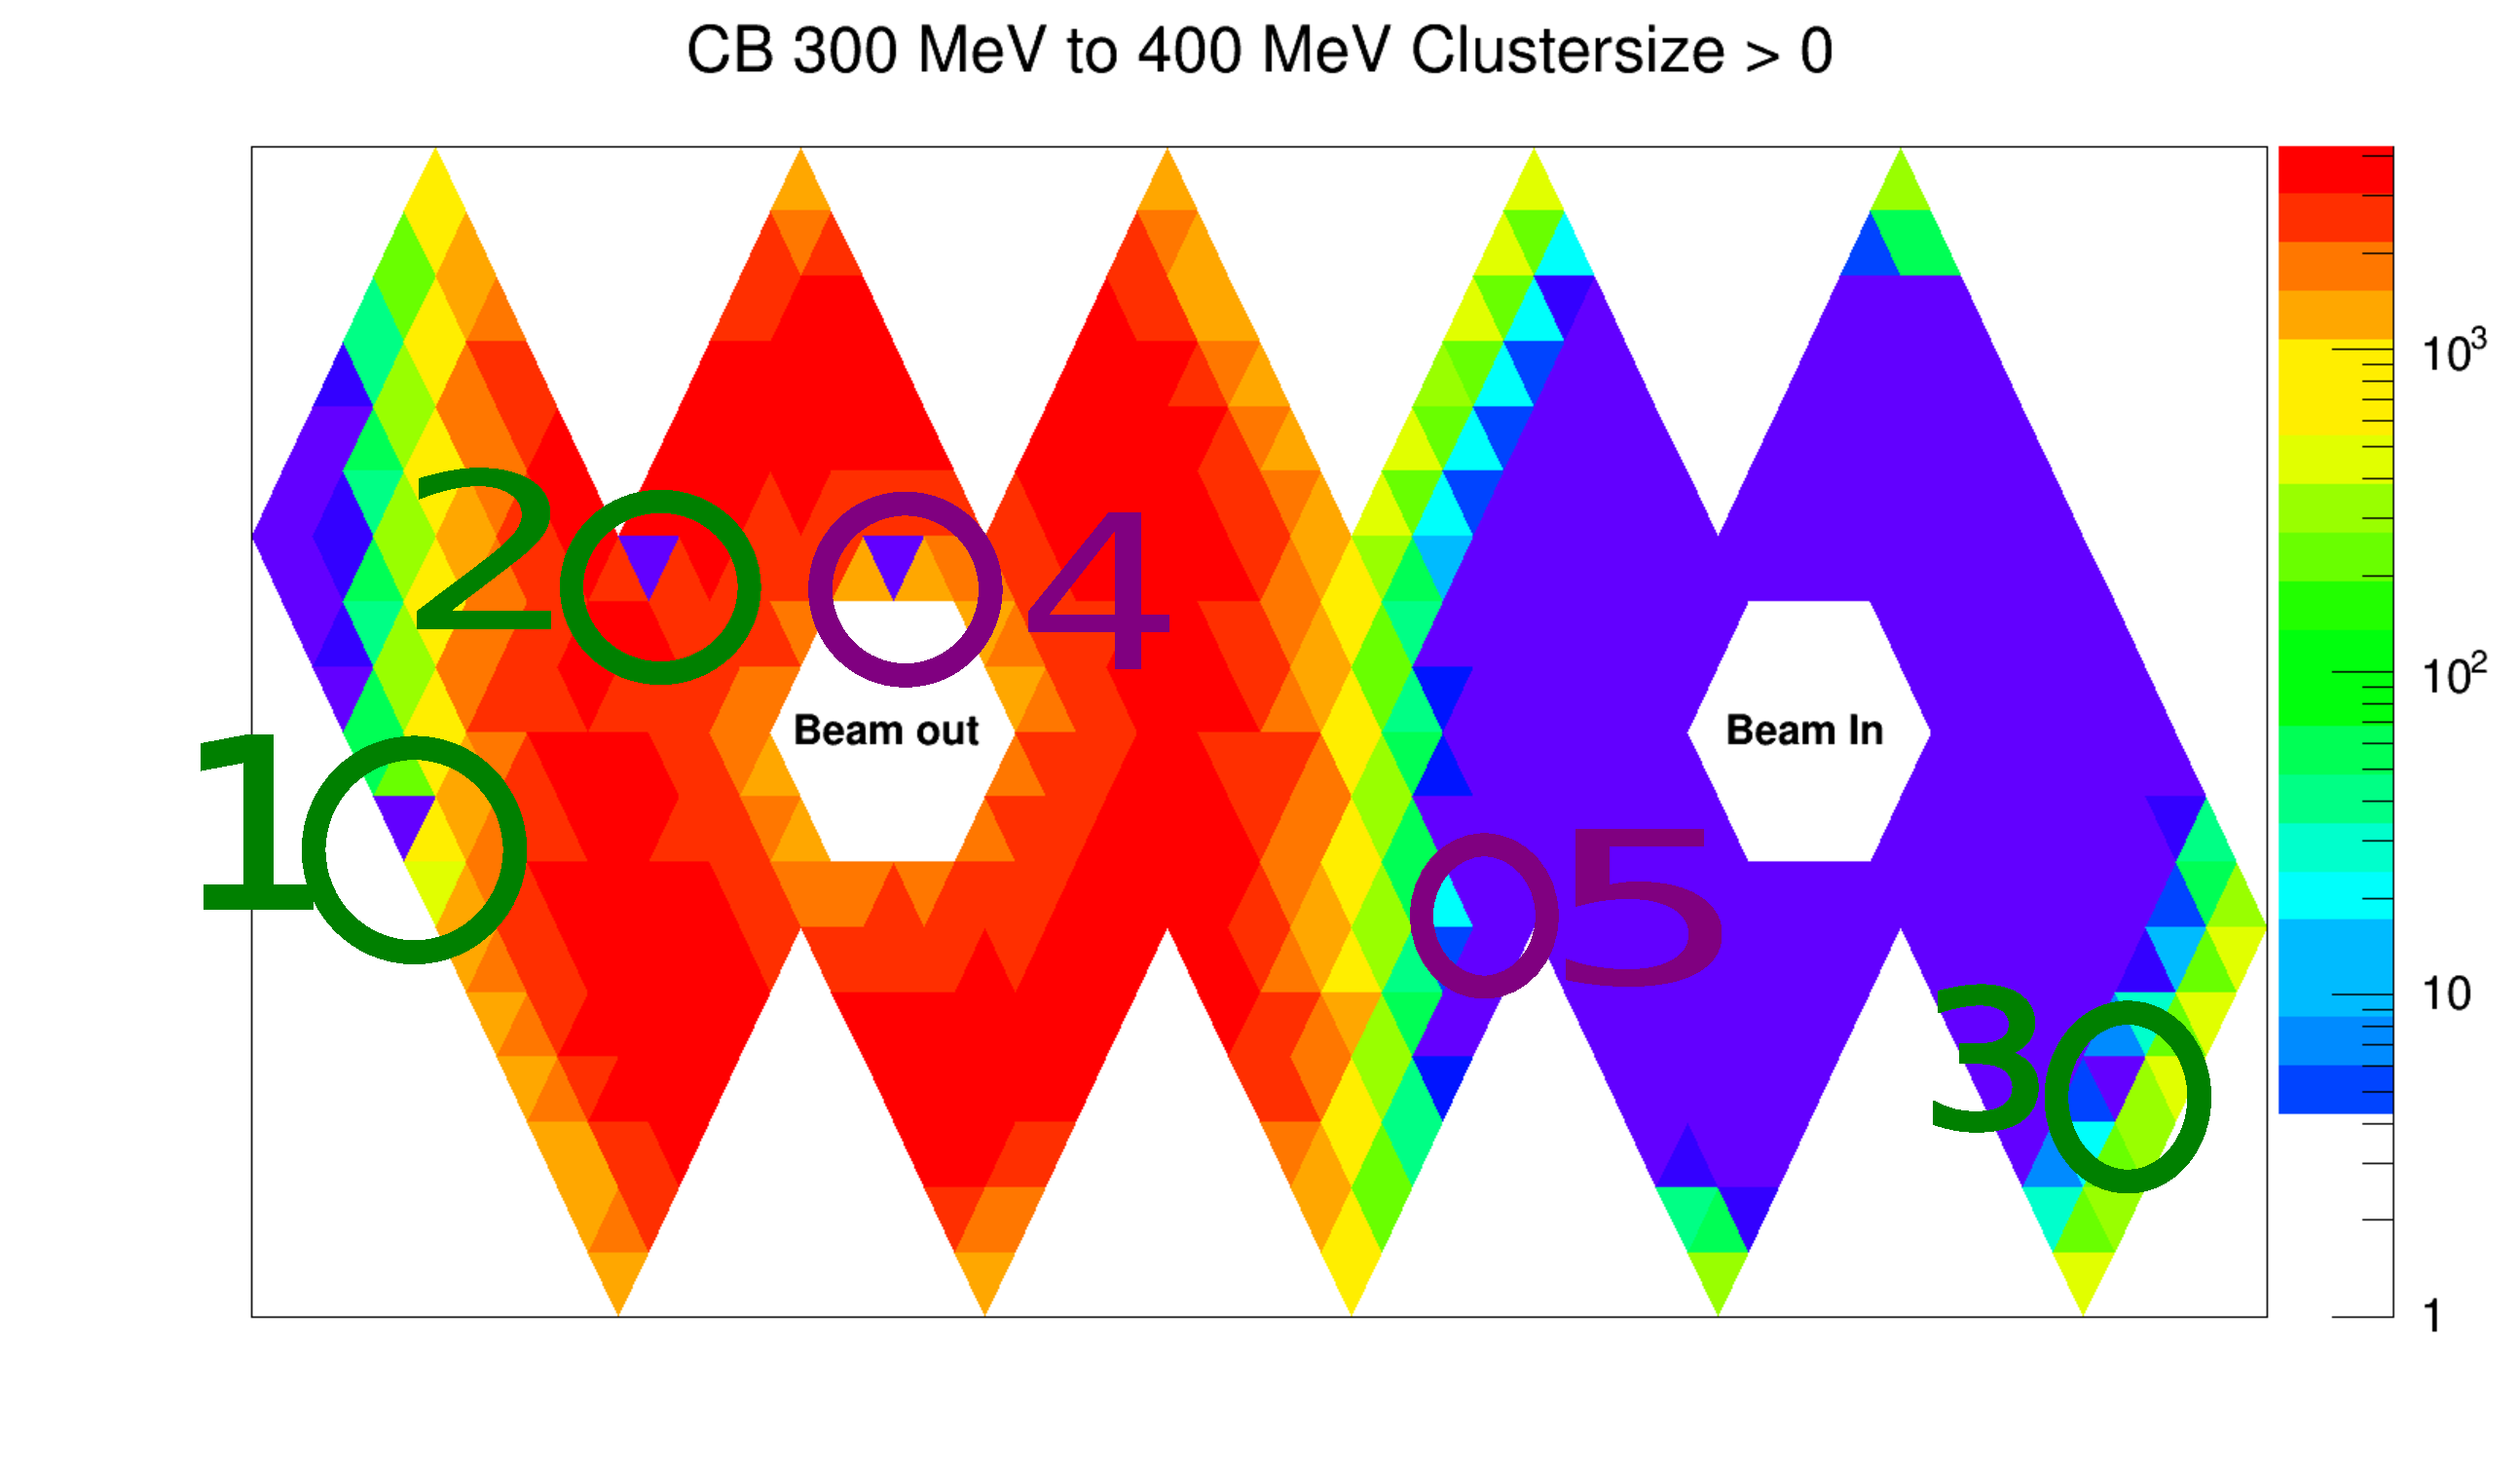
\includegraphics[width=74mm]{NewCalib/Strahlzeit2014/ClusterSizeNew/20172404MCClustersize0Map400MeV}
	\end{array}$
\end{center}
	\caption[Simulation: Markierte defekte Kristalle]{Daten aus der Strahlzeit: Es sind die gleichen Kristalle, wie in der vorherigen Abb. markiert. Allerdings sind die Kristalle die vorher rot markiert waren, hier gr\"un markiert, da man sie sonst nicht erkennen kann. Links besitzen die Photonen eine Energie von $0\,\text{MeV}$ bis $100\, \text{MeV}$ rechts von $300\,\text{MeV}$ bis $400\,\text{MeV}$.}
	\label{fig:MC-Karte-Dead-Crystals}
\end{figure}



Wenn man sich nun diese Karten mit durch Monte-Carlo generierten Daten anschaut (Abbildung: \ref{fig:MC-Karte-Dead-Crystals} links), f\"allt auf, dass die Nachbarn der toten Kristalle auch bei niedrigen Energien nicht aufleuchten. Sie verhalten sich, wie man es erwartet. Das hei{\ss}t, es ist sehr wahrscheinlich, dass die Auslese defekt ist. 

Die genaue Ursache dieses Ph\"anomens muss allerdings noch bestimmt werden.




\begin{figure}[h!]
\begin{center}
	$\begin{array}{cc}

		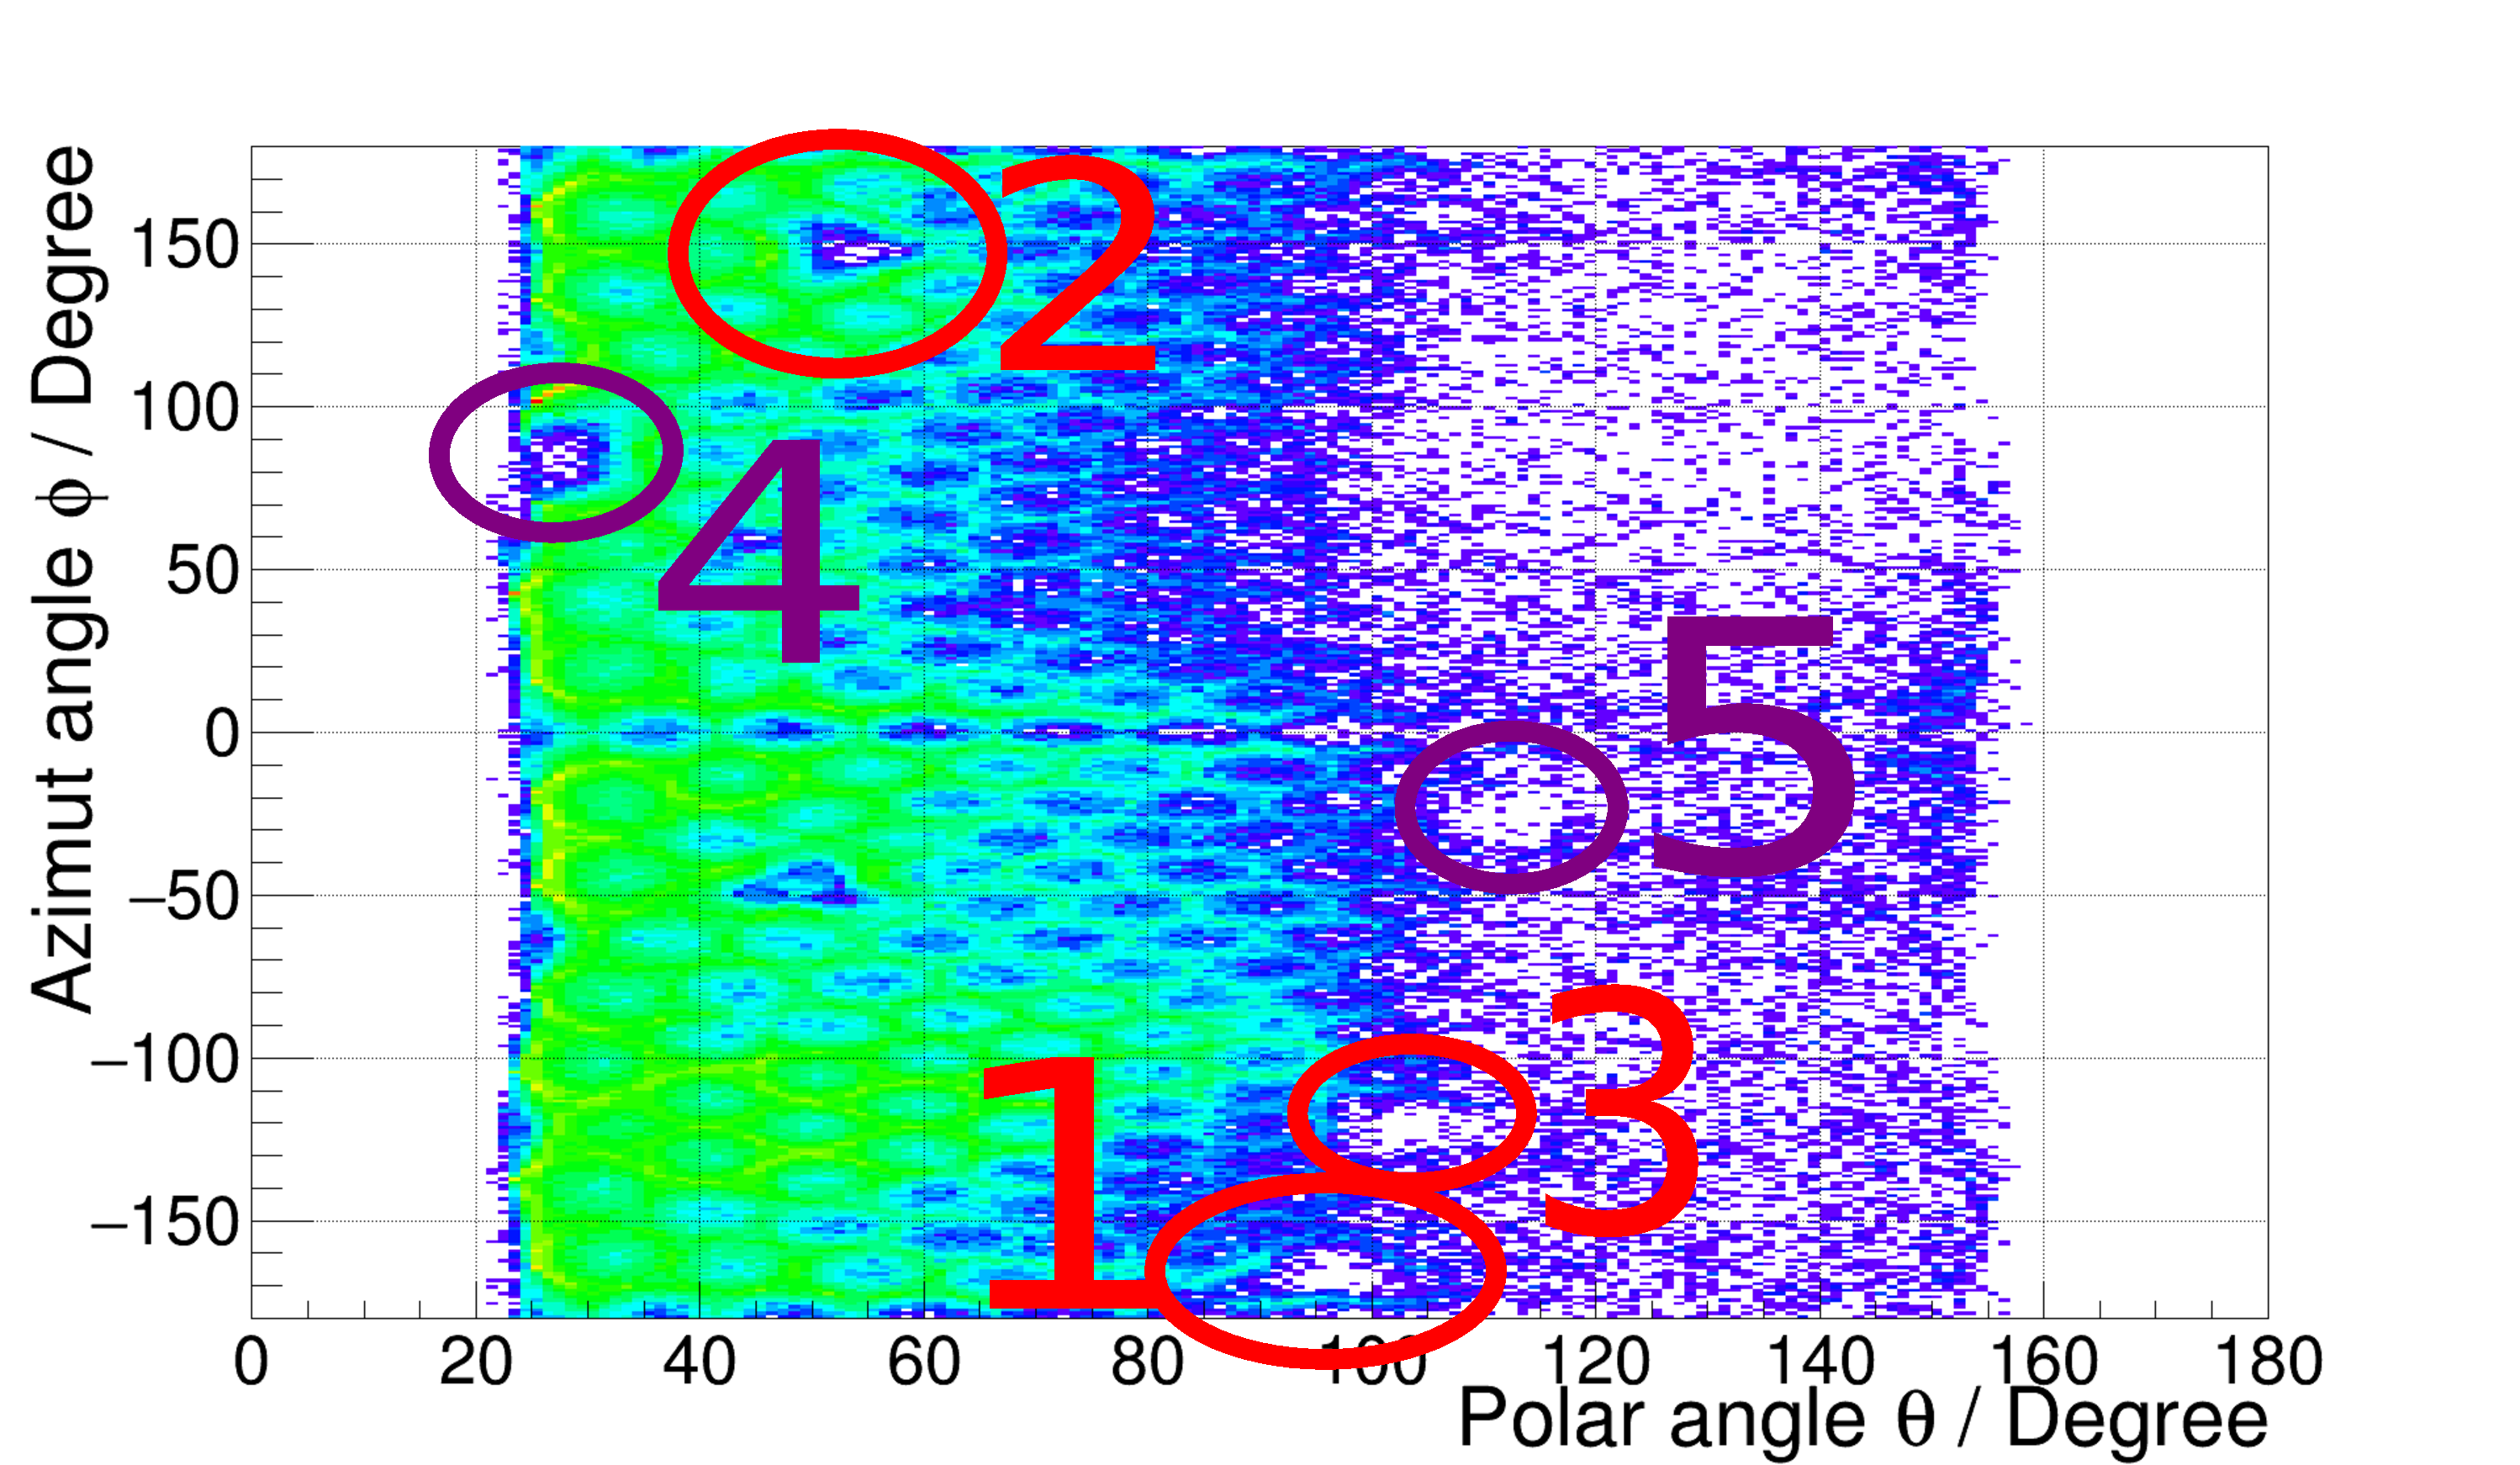
\includegraphics[width=74mm]{NewCalib/Strahlzeit2014/ClusterSize/20172104StrahlzeitDeadCrystalMarked}


		\includegraphics[width=74mm]{NewCalib/Strahlzeit2014/ClusterSizeNew/20172404Clustersize0Map400MeV}
\end{array}$
\end{center}
	\caption[Strahlzeit: Markierte defekte Kristalle; Hohe Energien]{Daten aus der Strahlzeit: Es wurden die gleichen Kristalle, wie in der vorherigen Abb. markiert, allerdings ist die Photonenenergie hier von $300\,\text{MeV}$ bis $400\,\text{MeV}$.}
	\label{fig:Strahlzeit-Dead-Crystals-Hohe-Energien}
\end{figure}

F\"ur h\"ohere Energien verhalten sich alle Nachbarn von den defekten Kristallen wie erwartet. Es ist kein aufleuchten mehr zu erkennen. Dies ist f\"ur Daten aus der Strahlzeit in Abbildung \ref{fig:Strahlzeit-Dead-Crystals-Hohe-Energien} und f\"ur Daten aus der Simulation in Abbildung \ref{fig:MC-Karte-Dead-Crystals} rechts zu sehen.

Da diese St\"orung auch nur f\"ur niedrige Energien auftritt, ist sie bei der Betrachtung der Abweichung vom $\pi^0$-Peak f\"ur Photonen mit \"ahnlicher Energie nicht weiter wichtig gewesen, da die starke Abweichung nur f\"ur Photonenenergien auftritt, die gr\"o{\ss}er als $300\,\text{MeV}$ sind.

Auch wenn man verlangt, dass die Clustergröße gr\"o{\ss}er als drei sein muss, das hei{\ss}t, jedes detektierte Teilchen muss mindestens vier Detektoren ausl\"osen, detektieren die Nachbarn der drei defekten Kristalle immer noch zu viele Events bei niedrigen Energien. Zu sehen in Abbildung \ref{fig:Strahlzeit-Clustersize3-Map} links. F\"ur hohe Energien ergibt sich durch diesen Schnitt keine Ver\"anderung. In der gleichen Abbildung rechts zu sehen.



\begin{figure}[h!]
	\begin{center}$
		\begin{array}{cc}


		\includegraphics[width=74mm]{NewCalib/Strahlzeit2014/ClusterSizeNew/20172404Clustersize3Map100MeV}
		

		\includegraphics[width=74mm]{NewCalib/Strahlzeit2014/ClusterSizeNew/20172404Clustersize3Map400MeV}
\end{array}$
\end{center}
	\caption[Strahlzeit: Markierte defekte Kristalle; Clustergröße $>$ 3]{Daten aus der Strahlzeit. Markiert sind die bereits bekannten defekten Kristalle. Allerdings gibt es hier die Bedingung, dass mindestens vier Detektoren bei einem Events ausgel\"ost werden m\"ussen.}
	\label{fig:Strahlzeit-Clustersize3-Map}
\end{figure}


\subsection{Vermutung f\"ur weitere defekte Kristalle}

Wie in Kapitel \ref{sec:Bekannte-Dead-Crystals} erw\"ahnt, sind f\"unf Detektoren bekannt, welche nicht richtig funktioniert haben, und deswegen ausgeschaltet sind. Allerdings fallen, zus\"atzlich zu diesen f\"unf Kristallen, noch weitere auf, welche ungew\"ohnlich wenig Events registrieren.
Die Karte, in der diese Kristalle markiert sind, ist in Abbildung \ref{fig:Vermutete-Dead-Crystals-Map} zu sehen.

\begin{figure}[h!]
	\begin{center}
		\includegraphics[width=100mm]{NewCalib/Strahlzeit2014/ClusterSizeNew/20172504StrahlzeitMoreDead}
	\end{center}
\caption[Strahlzeit: Vermutliche defekte Kristalle]{Daten aus der Strahlzeit: Markiert sind vermutete defekte Kristalle, die als solche noch nicht markiert wurden. Die Clustergröße muss gr\"o{\ss}er als drei sein.}
\label{fig:Vermutete-Dead-Crystals-Map}

\end{figure}

Hier sind vier weitere vermutliche defekte Kristalle markiert, die im Vergleich zu ihren Nachbardetektoren weniger Events registriert haben, als man erwarten w\"urde. Der durch die Nummer sechs markierte Kristall liegt direkt neben dem bereits als defekt markierten Kristall (markiert mit Nummer 4 in den Abbildungen aus Kapitel \ref{sec:Bekannte-Dead-Crystals} / Elementnummer 677). 
 
 Um nun leichter zu entscheiden, ob es sich bei den Detektoren wirklich um defekte Kristalle handelt, wird wieder eine Tabelle erstellt.
 
 
 \definecolor{Gray}{gray}{0.9}
\newcolumntype{g}{>{\columncolor{Gray}}c}
 \begin{table}[h!]
 \begin{center}
 	
 \begin{tabular}{lcc}
 
 	
 	Nummer in Abb. & Elementnummer&Anzahl der Events \\
	 
 	\hline
 	%\rowcolor{LightCyan}
 	6& \textcolor{red}{678} &\textcolor{red}{48} \\
 	 
 	 & 677&0 \\
 	
 	 & 676& 11808\\ 
 	
 	
 	\hline
 	7& \textcolor{red}{17} &\textcolor{red}{21} \\
 	
 	& 16 & 3311\\
 	
 	& 18& 7175 \\
 	
 	 & 19& 3439 \\
 	
 	\hline
 	
 	8 & \textcolor{red}{125} &\textcolor{red}{513} \\
 	
 	
 	 & 122& 6613\\
 	
 	 & 128 & 5307 \\
 	
 	& 126 & 4103 \\
 	
 	\hline
 	
 	9 & \textcolor{red}{89}& \textcolor{red}{2500}\\
 	
 	& 88& 8591\\
 	
 	&90&7975 \\
 	
 	&91&4652 \\
 	
 	
 	
 	\end{tabular}
 \caption[Strahlzeit: Vermutete defekte Kristalle und ihre Nachbarn mit Anzahl ihrer Events]{Daten aus der Strahlzeit: Tabelle mit weiteren vermutlichen defekten Kristallen (Rot markiert). Auch eingetragen sind die Anzahl der Events in den Detektoren. Schwarz geschrieben sind die Nachbarn der Detektoren.}
\label{tab:Vermutete-Dead-Crystals} 
\end{center}
 \end{table}
 
 In Tabelle \ref{tab:Vermutete-Dead-Crystals} sind die Detektoren rot aufgetragen, die vermutlich ebenfalls nicht wie gew\"unscht funktionieren. Ihre jeweiligen Nachbarn sind schwarz geschrieben. Die Vermutung, dass diese Detektoren defekt sind, entsteht dadurch, dass sie teilweise deutlich weniger Events registrieren als ihre Nachbarn. Der Nachbar mit der Elementnummer 677 stellt dabei eine Ausnahme dar, da dieser, wie in Kapitel \ref{sec:Bekannte-Dead-Crystals} bereits beschrieben, ein bekannter defekter Kristall ist und damit ausgeschaltet ist. Der Kristall 678 registriert allerdings nur 48 Events, w\"ahrend einer seiner Nachbar, welcher nicht als rauschender Kristall identifiziert wurde, \"uber $10^5$ Events detektiert. Bei einer so gro{\ss}en Abweichung muss man davon ausgehen, dass Kristall 678 nicht richtig funktioniert.  
 
 \"Ahnlich ist es auch bei den anderen Kandidaten. Zwar ist der Unterschied hier nicht so gro{\ss}, allerdings ist er immer noch sehr deutlich, sodass man diese Kristalle auch genauer untersuchen sollte.


\section{$\phi$-Verteilung im Crystal-Ball}

Auch ist die Verteilung, welche die Photonen im Crystal-Ball haben, sehr ungew\"ohnlich.

\begin{figure}[h!]
	\begin{center}
		\includegraphics[width=100mm]{NewCalib/ThetaPhiVerteilung/20172404ThetaPhi200MeVBeam}
		\caption[Strahlzeit: Verteilung der detektierten Photonen im CB]{Daten aus der Strahlzeit: Es handelt sich um Photonen mit einer Energie zwischen $200\,\text{MeV}$ und $225\,\text{MeV}$. Es ist die Verteilung der detektierte Photonen im Crystal-Ball dargestellt.}
		\label{fig:Verteilung-der-Photonen-im-CB}
	\end{center}
\end{figure}
Zu sehen ist diese Verteilung in Abbildung \ref{fig:Verteilung-der-Photonen-im-CB}. Eigentlich w\"urde man erwarten, dass sich die Photonen unabh\"angig vom $\phi$-Winkel im Raum verteilen. Das liegt daran, das der eingehende Photonenstrahl in $z$-Richtung verl\"auft, und damit werden alle anschlie{\ss}end entstehenden Teilchen in $z$-Richtung geboostet. Folglich sind sie unabh\"angig von $\phi$. 
Allerdings sieht man in dieser Abbildung, dass die meisten Teilchen in der unteren H\"alfte des Crystal-Balls bei einem $\phi$-Winkel von ca. -100$^{\circ}$ detektiert werden.

%Als Ursache f\"ur diese Verteilung werden die Neutronen vermutet, die durch hochenergetische Elektronen im Beam-Dump ausgel\"ost werden. 

Dass es sich hierbei um einen rauschenden Kristall handelt, ist sehr unwahrscheinlich, da sehr viele Kristalle betroffen sind.

Auch hierf\"ur muss die genaue Ursache noch herausgefunden werden.


%_______________________________________________________________________________
\chapter{Zusammenfassung und Ausblick}
\label{chap:Zusammenfassung}

Diese Arbeit beschreibt verschiedene Studien, die durchgef\"uhrt werden, um die Ursache einer energieab\"angigen Abweichung der berechneten invarianten Masse des $\pi^0$ f\"ur hohe Photonenenergien zu bestimmen. 

Dazu m\"ussen verschiedene Vorbereitungen getroffen werden, um diese Studien durchzuf\"uhren. Um eine Aussage \"uber die Energieabh\"angigkeit des Detektors treffen zu k\"onnen, darf man nur Photonen betrachten, deren Energie sich \"ahnelt, da man sonst nicht wei{\ss}, welcher Effekt durch welche Energie verursacht wird. Dies ist eine sehr einschränkende Bedingung, welche nur sehr wenige Ereignisse erf\"ullen. So muss f\"ur die Analyse mit simulierten Daten ein neuer Ereignisgenerator geschrieben werden, um unn\"otig lange Simulationen zu vermeiden.

Bereits mit Daten aus der Strahlzeit wird beobachtet, dass die errechneten invarianten Masse des $\pi^0$ mit steigender Photonenenergie immer mehr von der tats\"achlichen $\pi^0$ Masse abweicht. Als Grund werden zun\"achst die Detektoren am Rand des Strahlenein- und -ausgangs des Crystal-Balls vermutet. Diese k\"onnen nur sehr schwer kalibriert werden, da sie nicht zu allen Seiten Nachbarkristalle besitzen. Somit kann die Energie des elektromagnetischen Schauers, welcher sich ausl\"ost, wenn diese Detektoren getroffen werden nicht vollst\"andig rekonstruiert werden. Deswegen entschied man sich dazu, die Prozesse zu verwerfen, in denen mindestens ein Photon diese Randkristalle trifft. Diese Bedingung bringt eine leichte Verbesserung, allerdings nimmt immer noch die Abweichung mit steigender Photonenenergie weiter zu.

Deswegen wird in den n\"achsten Studien auf die Simulation zur\"uckgegriffen. Auch hier gibt es eine energieabh\"angige Abweichung der errechneten $\pi^0$ Masse zur eigentlichen $\pi^0$ Masse. Allerdings zeigt sich hier keine Verbesserung durch die Bedingung, dass die Detektoren am Rand vernachl\"assigt werden.

Mit den weiteren Studien sollen die Auswirkungen verschiedener Bedingungen auf die Abweichung untersucht werden.

Die Forderung, dass der \"Offnungswinkel zwischen den beiden Photonen mindestens 30$^{\circ}$ betr\"agt, damit eine zu starke Cluster \"Uberlagerung vermieden wird, brachte keine Verbesserung, da keine hochenergetischen Photonen mehr registriert werden. 

Die Betrachtung eines $\pi^0$, welches im Ursprung zerf\"allt und anschlie{\ss}end in eine zuf\"allige Richtung geboostet wird, bringt ebenfalls die gleiche Form der Abweichung.

Weiter werden verschiedene Studien durchgef\"uhrt, um die Auswirkung der Geometrie und Aufl\"osung des Detektors besser zu verstehen. So wird die invariante Masse f\"ur verschiedene $z$-Vertices des Targets berechnet. Das hei{\ss}t, wie verh\"alt sich die Abweichung, wenn das Teilchen am Anfang, Ende oder im Ursprung zerf\"allt. Dies f\"uhrt zu einer Auff\"acherung der Abweichung, da zur Berechnung der invarianten Masse angenommen werden muss, dass das $\pi^0$ im Ursprung zerf\"allt. Folglich unterscheiden sich die errechneten und die tats\"achlichen \"Offnungswinkel. Dies wird auch noch einmal extra untersucht mit dem Ergebnis, dass in der Regel für hohe Photonenenergien ein zu großer Öffnungswinkel berechnet wird, wodurch schließlich eine zu große invariante Masse berechnet wird. 
Leider konnte die Ursache im Rahmen dieser Arbeit nicht bestimmt werden.
\newline

Auch traten weitere Probleme auf, die noch genauer untersucht werden m\"ussen. So verhalten sich manche Kristalle \"au{\ss}erst ungew\"ohnlich im Bereich niedriger Energien. Auch werden manche Kristalle gefunden, die weniger Events registrieren als erwartet. Die Auslese dieser Kristalle muss deswegen \"uberpr\"uft werden. 

Au{\ss}erdem wird eine sehr ungew\"ohnliche $\phi$-Verteilung der detektierten Teilchen im Crystal-Ball beobachtet.




%In der Zusammenfassung sollten Sie in knapper Form die Aufgabenstellung 
%und die wichtigsten Ergebnisse rekapitulieren. Es ist f\"ur die 
%Gutachter hilfreich, wenn Sie ausdr\"ucklich beschreiben, worin 
%Ihre eigenen Beitr\"age liegen. Scheuen Sie sich auch nicht davor 
%auszusprechen, welche Untersuchungen durch die Zeitbegrenzung der 
%Bachelorarbeit nicht m\"oglich waren und nutzen Sie dies als 
%\"Uberleitung zu einem Ausblick auf m\"ogliche weitergehende 
%Arbeiten an der Aufgabenstellung.

%_______________________________________________________________________________
\begin{appendix}
\chapter{Anhang}
\section{Herleitung der Formel zur Berechnung der invarianten Masse}
\label{sec:Herleitung-der-Formel-zur-Berechnung-der-invarianten-Masse}

Man betrachte die drei Viererimpulse f\"ur den Prozess: $\pi^0\rightarrow \gamma\gamma $
\begin{equation}
p_{\pi^0}^{\mu}=\left(\begin{array}{c}E_{\pi^0}\\\vec{p}_{\pi^0}\end{array}\right) \textnormal{,}\,\,
p_{1}^{\mu}=\left(\begin{array}{c}E_{1}\\\vec{p}_{1}\end{array}\right) \,\textnormal{und}\,\, p_{2}^{\mu}=\left(\begin{array}{c}E_{2}\\\vec{p}_{2}\end{array}\right)
\end{equation}

Dabei sind $E_{1}$ und $E_{2}$ die Energien und $\vec{p_{1}}$ und $\vec{p_{2}}$ die Impulse der beiden Photonen und $E_{\pi^0}$ die Energie und $\vec{p}_{\pi^0}$ der Impuls des Pion.

Aufgrund der Energie- und Impulserhaltung gilt:
\begin{equation}
p^{\mu}_{\pi^0} = p^{\mu}_1 + p^{\mu}_2
\end{equation}

Diese Gleichung kann nun quadriert werden:

\begin{equation}
\begin{split}
\rightarrow \underbrace{p^{\mu^2}_{\pi^0}}_{m_{\pi^0}^2}=& (p_{1}^{\mu}+p_{2}^{\mu})^2 \\ 
\rightarrow m_{\pi^0}^2=& \underbrace{p_{1}^{\mu^2}}_{=m_1^2}+\underbrace{p_{2}^{\mu^2}}_{=m_2^2}-2p_{1}^{\mu}p_{2}^{\mu} \\ 
=& m_1^2+m_2^2-2E_1E_2+2\vec{p}_1\vec{p}_2 \\ 
=& m_1^2+m_2^2-2E_1E_2+2|\vec{p}_1| |\vec{p}_2| \cos(\alpha) \\
&\textnormal{mit } \alpha=\sphericalangle(\vec{p}_1,\vec{p}_2)
\end{split}
\end{equation}

Da man sich nur f\"ur die Photonen interessiert, kann angenommen werden, dass es sich bei den Teilchen um Photonen handelt. Daraus folgt, dass $|\vec{p}_1|=E_1$ und $|\vec{p}_2|=E_2$ und $m_1=m_2=0$ gilt.

Damit lässt sich die invariante Masse des Pions, welches in die beiden Photonen zerfallen ist, durch
\begin{equation}
\begin{split}
\Rightarrow{m_{\pi^0}=\sqrt{2E_1E_2(1-\cos(\alpha))}}
\label{eq:Formel-zur-Berechnung-der-Invariante-Masse-Herleitung}
\end{split}
\end{equation}
berechnen.

Durch den Crystal-Ball sind alle Variablen in dieser Gleichung bekannt. So kann die Energie der Photonen bestimmt werden und durch Kenntnis der Azimut- und Polarwinkel der Photonen im Crystal-Ball kann der Winkel zwischen den beiden Photonen errechnet werden. Dazu muss allerdings angenommen werden, dass das $\pi^0$ im Zentrum des Targets zerfällt. Siehe dazu Kapitel \ref{sec:Z-Vertex-Abhaengigkeit}.

\section{Abbildungen}

%In der Regel sind die in Tabellen und Abbildungen enthalten Informationen 
%so wichtig, dass sie im Hauptteil der Arbeit erscheinen sollten. Unter 
%Umst\"anden sind aber erg\"anzende Tabellen und Abbildungen gut in einem 
%Anhang aufgehoben. Wie im Hauptteil sollten Sie auch hier darauf achten, 
%dass die in Tabellen und Figuren (siehe Abb.\ \ref{Abb:1}) dargestellte 
%Information im Text angesprochen wird und selbsterkl\"arende Legenden 
%vorhanden sind.
%\medskip
\begin{comment}

\begin{figure}[h!]
	\begin{center}
		\includegraphics[width=100mm]{NewCalib/Strahlzeit2014/20171904RealIntervalAllFits}
		\caption[Strahlzeit: Symmetrische Photonen alle Fits mit Hintergrund]{Alle Fits der Energieintervalle mit der Bedingung, dass sich die Photonen sich energetisch ähneln.}
		\label{fig:similarenergyallfits}
	\end{center}
\end{figure}
\end{comment}


\begin{figure}[h!]
	\begin{center}
		\includegraphics[width=100mm]{20170405StrahlzeitNoCutAllFits}
		\caption[Strahlzeit: Alle Fits keine weiteren Bedingungen]{Alle Fits der Energieintervalle mit der Bedingung, dass sich die Photonen sich energetisch ähneln und dass die detektierten Teilchen ungeladen sind. Es wurde der Bereich mit dem $\pi^0$-Peak vergr\"o{\ss}ert.}
		\label{fig:similarenergyallfitsuncharged}
	\end{center}
\end{figure}

\begin{comment}

\begin{figure}[h!]
	\begin{center}
		\includegraphics[width=100mm]{201728104StrahlzeitNoCutUnzoomed}
		\caption[Strahlzeit: Unzoomed Abweichung]{Daten aus der Strahlzeit: Nicht vergrößert; Abweichung}
		\label{fig:Unzoomed}
	\end{center}
\end{figure}
\end{comment}



\begin{figure}[h!]
	\begin{center}
		\includegraphics[width=100mm]{NewCalib/Strahlzeit2014/20171904Real30DegreeCutHist}
		\caption[Strahlzeit: 2D-Hist ohne Detektoren am Rand]{Daten aus der Strahlzeit: Die Detektoren am Rand werden vernachl\"assigt. Die Energie der Photonen aus einem Zerfall muss sich \"ahneln.}
		\label{fig:30-Degree-Cut-Histogramm}
	\end{center}
\end{figure}


\begin{figure}[h!]
	\begin{center}
		\includegraphics[width=100mm]{20170405Strahlzeit30DegreeCutAllFits}
		\caption[Strahlzeit: Ohne Detektoren am Rand; alle Fits]{Alle Fits der Energieintervalle mit den Bedingungen, dass sich die Photonen sich energetisch ähneln und dass die detektierten Teilchen ungeladen sind. Au{\ss}erdem wurden die Detektoren am Rand vernachl\"assigt.}
		\label{fig:30-Degree-Cut-RealData-All-Fits}
	\end{center}
\end{figure}






\begin{figure}[h!]
	\begin{center}
		\includegraphics[width=100mm]{NewCalib/20171904Sim30DegreeCut}
		\caption[Simulation: 2D-Hist; Ohne Detektoren am Rand]{Zweidimensionales Histogramm mit simulierten Daten. Die Energie der detektierten Photonen musste \"ahnlich sein, au{\ss}erdem wurden die Detektoren am Rand nicht ber\"ucksichtigt.}
		\label{fig:Sim-Data-2DHist-30-Degree-Edge}
	\end{center}
\end{figure}




\begin{figure}[h!]
	\begin{center}
		\includegraphics[width=100mm]{20170505MinOpeningAngle2DHist}
		\caption[Simulation: 2D-Hist \"Offnungswinkel muss gr\"o{\ss}er als 30$^{\circ}$ sein.]{Zweidimensionales Histogramm mit simulierten Daten. Der \"Offnungswinkel zwischen den beiden durch den Zerfall entstandenen Photonen muss gr\"o{\ss}er als 30$^{\circ}$ sein.}
		\label{fig;2D-Hist-Min-OpeningAngle}
	\end{center}
\end{figure}






\begin{comment}
	
\begin{figure}[h!]
	\begin{center}
		\includegraphics[width=100mm]{NewCalib/20171904Sim30DegreeCutAllFits}
		\caption[Simulation: Alle Fits ohne Detektoren am Rand]{Alle Fits zu den Simulierten Daten mit der Bedingung, dass die Photonen eine \"ahnliche Energie besitzen m\"ussen. Au{\ss}erdem werden die Detektoren am Rand ber\"ucksichtigt.}
		\label{fig:Sim-30-Degree-Cut-All-Fits}
	\end{center}
\end{figure}

\end{comment}


\begin{figure}[h!]
	\begin{center}
		\includegraphics[width=100mm]{NewCalib/UrsprungIsotrop/20171904SimUrsprungIsotropNoCutHist}
		\caption[Simulation: 2D-Hist Isotroper Boost im Ursprung ]{Zweidimensionales Histogramm mit Simulierten Daten. Die Pionen sind isotrop im Ursprung zerfallen und erhalten einen Boost in eine zuf\"allig bestimmte Richtung. Die Energie der detektierten Photonen muss \"ahnlich sein.}
		\label{fig:Sim-Data-Ursprung-2DHist-No-Cut}
	\end{center}
\end{figure}
\begin{comment}

\begin{figure}[h!]
	\begin{center}
		\includegraphics[width=100mm]{NewCalib/UrsprungIsotrop/20171904SimIsotropUrsprungNoCutAllFits}
\caption[Simulation: Isotroper Boost im Ursprung alle Fits]{Alle Fits mit der Bedingung, dass das $\pi^0$ im Ursprung zerf\"allt, und in eine zuf\"allige Richtung geboostet wird. }
\label{fig:All-Fits-Isotrop-No-Cut}
\end{center}

\end{figure}
\end{comment}

\begin{figure}[h!]
	\begin{center}
		\includegraphics[width=100mm]{NewCalib/UrsprungIsotrop/20171904SimUrsprungIsotrop30DegreeCutHist}
		\caption[Simulation: 2D-Hist Isotroper Boost im Ursprung ohne Detektoren am Rand]{Zweidimensionales Histogramm mit Simulierten Daten. Die Pionen sind isotrop im Ursprung zerfallen und erhielten einen Boost in eine zuf\"allig bestimme Richtung. Die Energie der detektierten Photonen muss \"ahnlich sein, au{\ss}erdem werden die Detektoren am Rand nicht ber\"ucksichtigt.}
		\label{fig:Sim-Data-Ursprung-2DHist-30-Degree-Edge}
	\end{center}
\end{figure}

\begin{comment}
\begin{figure}[h!]
	\begin{center}
		\includegraphics[width=100mm]{NewCalib/UrsprungIsotrop/20171904SimIsotropUrsprung30DegreeCutAllFits}
		\caption[Simulation: 2D-Hist Isotroper Boost im Ursprung ohne Detektoren am Rand alle Fits]{Alle Fits mit der Bedingung, dass das $\pi^0$ im Ursprung zerf\"allt, und in eine zuf\"allige Richtung geboostet wird. Die Detektoren am Rand wurden nicht ber\"ucksichtigt.}
	\end{center}
	
\end{figure}
Inhalt...
\end{comment}


\begin{figure}[h!]
	\begin{center}
		\includegraphics[width=100mm]{20172804IsotropUrsprungFitFail}
		\end{center}
	\caption[Simulation: Fehlgeschlagener Fit Isotrop Urspung]{Daten aus der Simulation: \textit{Fehlgeschlagener} Fit f\"ur isotropen Zerfall im Ursprung.}
	\label{fig:Isotrop-Fit-Fail}
\end{figure}



\begin{figure}[h!]
	\begin{center}
		\includegraphics[width=100mm]{AngleRegGen/20171804TrueCandsAngleDeviation}
		\caption[Simulation: Winkel zwischen gen. und rek. Photon]{Daten aus der Simulation: Zu sehen ist der Winkel zwischen dem generiertem und dem entsprechendem rekonstruiertem Photon f\"ur verschiedene Energien.}
		\label{fig:Angle-Rec-Gen-Hist}
	\end{center}
\end{figure}





\begin{figure}[h!]
	\begin{center}
		\includegraphics[width=100mm]{NewCalib/20171904SimOpeningAngleDeviation}
		\caption[Simulation: Unterschied zwischen dem rek. und den gen. \"Offnungswinkel]{Daten aus der Simulation: Zu sehen ist der Unterschied zwischen dem tats\"achlichem und dem errechneten \"Offnungswinkel f\"ur verschiedene Photonenenergien.}
		\label{fig:Unterschied-Rec-Gen-Opening-Angle}
	\end{center}
\end{figure}


\begin{figure}[h!]
	\begin{center}
		\includegraphics[width=100mm]{NewCalib/20171904SimZVertex3DHist}
		\caption[Simulation: 3D-Hist Z-Vertex]{Daten aus der Simulation: Darstellung der Abh\"angigkeit der errechneten $\pi^0$-Masse (x-Achse) von der Energie der detektierten Photonen (y-Achse) und dem Ort an dem das $\pi^0$ im Target zerfallen ist (z-Achse).
		Leider war es nicht m\"oglich dieses Histogramm besser darzustellen}
	\label{fig:Z-Vertex-3D-Hist}
	\end{center}
\end{figure}

\begin{comment}
\begin{figure}[h!]
	\begin{center}
		\includegraphics[width=100mm]{NewCalib/20171904ZVertexAllFits}
		\caption[Simulation: Z-Vertex alle Fits]{Alle Fits f\"ur die Betrachtung der Z-Vertex Abh\"angigkeit. In jeder Zeile ist ein einzelnes Z-Vertex-Intervall aufgetragen. Die Detektoren am Rand wurden ber\"ucksichtigt}
		\label{fig:ZVertex-All-Fits}
	\end{center}
\end{figure}
Inhalt...
\end{comment}

\begin{figure}[h!]
	\begin{center}
		\includegraphics[width=100mm]{NewCalib/20171904SimMinOpeningAngleHist}
		\caption[Simulation: 2D-Hist \"Offnungswinkel $>$ 30$^{\circ}$]{Histogramm mit der Bedingung, dass der \"Offnungswinkel zwischen den beiden detektierten Photonen mindestens 30$^\circ$ betr\"agt.}
	\end{center}
\end{figure}
\begin{comment}
\begin{figure}[h!]
	\begin{center}
		\includegraphics[width=100mm]{NewCalib/20171904SimMinOpeningAngleAllFits}
		\caption[Simulation: \"Offnungswinkel $>$ 30$^{\circ}$ alle Fits]{Alle Fits f\"ur die Bedingung, dass der \"Offnungswinkel zwischen den detektierten Teilchen mindestens $30^{\circ}$ betr\"agt.}
		\label{fig:Relative-Abweichung-Min-Opening-Angle-AllFits}
	\end{center}
\end{figure}
Inhalt...
\end{comment}


\begin{figure}[h!]
	\begin{center}
		\includegraphics[width=100mm]{OeffZVertex/20170205DiffOeffZVertex-4}
		\caption[Simulation: Differenz zwischen rek. und gen. \"Offnungswinkel: Zerfall am Anfang des Targets]{Daten aus der Simulation: Differenz zwischen rekonstruiertem und generiertem \"Offnungswinkel f\"ur verschiedene Photonenenergien. Zerfall am Anfang des Targets.}
		\label{fig:OeffZVertex-4}
	
	\end{center}
\end{figure}

\begin{figure}[h!]
	\begin{center}
		\includegraphics[width=100mm]{OeffZVertex/20170205DiffOeffZVertexUrsprung}
		\caption[Simulation: Differenz zwischen rek. und gen. \"Offnungswinkel: Zerfall im Ursprung des Targets]{Daten aus der Simulation: Differenz zwischen rekonstruiertem und generiertem \"Offnungswinkel f\"ur verschiedene Photonenenergien. Zerfall im Ursprung des Targets.}
		\label{fig:OeffZVertex0}
		
	\end{center}
\end{figure}

\begin{figure}[h!]
	\begin{center}
		\includegraphics[width=100mm]{OeffZVertex/20170205DiffOeffZVertex+4}
		\caption[Simulation: Differenz zwischen rek. und gen. \"Offnungswinkel: Zerfall am Ende des Targets]{Daten aus der Simulation: Differenz zwischen rekonstruiertem und generiertem \"Offnungswinkel f\"ur verschiedene Photonenenergien. Zerfall am Ende des Targets.}
		\label{fig:OeffZVertex4}
		
	\end{center}
\end{figure}

\listoffigures



\listoftables
%_______________________________________________________________________________
%\section{Weiterf\"uhrende Details zur Arbeit}

%Manch wichtiger Teil Ihrer tats\"achlichen Arbeit ist zu technisch 
%und w\"urde den Hauptteil des Textes un\"ubersichtlich machen, 
%beispielsweise wenn es um die Details des Versuchsaufbaus in einer 
%experimentellen Arbeit oder um den f\"ur eine numerische Auswertung 
%verwendeten Algorithmus geht. Dennoch ist es sinnvoll, entsprechende 
%Beschreibungen in einem Anhang Ihrer Bachelorarbeit aufzunehmen. 
%Insbesondere f\"ur zuk\"unftige Arbeiten, die an Ihre Bachelorarbeit 
%anschlie{\ss}en, sind dies manchmal hilfreiche Informationen.

%_______________________________________________________________________________
%\chapter{Literaturverzeichnis}

%Machen Sie genaue Angaben, so dass die verwendeten Literaturstellen 
%eindeutig identifiziert und aufgefunden werden k\"onnen.
%Bei Lehrb\"uchern \cite{Weinberg:1995mt} ist es sinnvoll, 
%den Titel anzugeben, eventuell auch die Ausgabe. Bei Artikeln in 
%Fachzeitschriften \cite{Moch:2001zr} ist es \"ublich, nur die 
%gebr\"auchlichen Abk\"urzungen f\"ur den Titel der Zeitschrift, Band, 
%Erscheinungsjahr und Seite anzugeben. Unter Umst\"anden kann es auch 
%sinnvoll sein, im Internet aufgefundene Informationsquellen anzugeben, 
%zum Beispiel f\"ur Software \cite{LoopTools} oder zu den Details von 
%Ergebnissen gro{\ss}er experimenteller Kollaborationen. Es ist 
%selbstverst\"andlich, dass Sie auch Bachelor- \cite{BA:Freund}, 
%Diplom- oder Doktorarbeiten angeben, wenn Sie diese in Ihrer eigenen 
%Arbeit verwendet haben.
%\medskip



\renewcommand{\bibname}{\bfont Literaturverzeichnis} 
\bibliographystyle{h-physrev3}
\begin{thebibliography}{99}
\bibitem[Ant17]{Ant17} Github Internetseite der A2-Kollaboration, \url{https://github.com/A2-Collaboration-dev/ant/}, (Stand: 02.05.2017)

\bibitem[Ca10]{Ca10} Luigi Capozza, {\em Untergrundstudien zur Messung der
	Strangeness-Vektorformfaktoren
	des Protons durch parit\"atsverletzende
	Elektronenstreuung unter R\"uckw\"artswinkeln}, Dissertation, Universität Mainz, 2010 


\bibitem[Ce97]{Ce97} Brun, R. and Rademakers, F., \textit{ROOT: An object oriented data analysis framework}, \url{http://root.cern.ch}, 1997 

\bibitem[Ce15]{Ce15} Hilfeseite für die Crystal-Ball Funktion in ROOT, \url{https://root.cern.ch/root/html/tutorials/math/CrystalBall.C.html} (Stand: 27.04.2017)

\bibitem[Ce17]{Ce17} Hilfeseite f\"ur Zufallsgeneratoren in ROOT, \url{https://root.cern.ch/doc/master/classTRandom.html#a2007ae15ce828266aecb783ed3410e8b} (Stand: 11.04.2017)


\bibitem[De15]{De15} Skript \& Übungsblätter zur Vorlesung Experimentalphysik Vb WS15/16 Johannes-Gutenberg Universit\"at Mainz, Prof. Denig, \url{https://reader.uni-mainz.de/WiSe2015-16/08-128-055-00/_layouts/15/start.aspx#/Lists/DocumentLib/Forms/AllItems.aspx?RootFolder=}, (Stand: 14.03.2017)

\bibitem[Ge04]{Ge04} S. Agostinelli and J. Allison, \textit{Geant4 — A simulation toolkit}, Seiten 250 - 303, \url{http://geant4.cern.ch/}


\bibitem[KPh04]{KPh04} Prospekt des Institut für Kernphysik, Internetseite \url{https://portal.kph.uni-mainz.de/de/information/introduction/prospekt.pdf}, (Stand: 04.03.2017)

\bibitem[KPh07]{KPh07} Pressemitteilung der KPh, \url{https://www.uni-mainz.de/presse/archiv/zope.verwaltung.uni-mainz.de/presse/mitteilung/2007/2007_10_05_phys_einweihung_mami/showArticle_dtml.html}, (Stand 06.03.2017)


\bibitem[KPh11B]{KPh11B} Internetseite der Kernphysik {\em Betrieb}, Internetseite \url{http://www.kernphysik.uni-mainz.de/377.php}, (Stand: 26.04.2017)


\bibitem[KPh11F]{KPh11F} Internetseite der Kernphysik {\em Funktionsprinzip des MAMI}, Internetseite \url{http://www.kernphysik.uni-mainz.de/375.php}, (Stand: 06.03.2017)


\bibitem[KPh11G]{KPh11G} Internetseite der Kernphysik {\em Mainzer Mikrotron-Geschichte}, Internetseite \url{http://www.kernphysik.uni-mainz.de/379.php}, (Stand: 04.03.2017)


\bibitem[KPh16]{KPh16} Internetseite der A2-Kollaboration {\em Reelle Photonen}
Internetseite, \url{http://www.kph.uni-mainz.de/a2.php} (Stand: 11.03.2017)


\bibitem[Leo87]{Leo87} William R. Leo, \textit{Techniques for Nuclear and Particle Physics Experiments}, Springer, 1987

\bibitem[NBI15]{NBI15} Einf\"uhrung in die Programmierung mit ROOT von Manuel Calderon de la Barca Sanchez, \url{http://www.nbi.dk/~petersen/Teaching/Stat2015/PythonRootIntro/ROOT_TipsAndTricks.pdf} (Stand: 27.03.2017)


\bibitem[Ne17]{Ne17} Andreas Neiser, {\em Prototype development for a new readout of the CB/A2 setup and Measurement of the relative branching fraction of the $\eta' \rightarrow \omega \gamma$ decay}, Dissertation, Universität Mainz, 2017

\bibitem[PDG16]{PDG16} Olive, K. A. und andere, {\em Review of Particle Physics}, Chin. Phys., 2014

\bibitem[Pl07]{Pl07} Frohlich, I. und andere, \textit{Pluto: A Monte Carlo Simulation Tool for Hadronic
	Physics}, PoS,

	
\bibitem[Un04]{Un04} Marc Unverzagt, {\em Energie-Eichung des Crystal-Ball-Detektors am MAMI}, Diplomarbeit, Universität Mainz, 2004

\bibitem[Un08]{Un08} Marc Unverzagt, {\em Bestimmung des Dalitz-Plot-Parameters $\alpha$ für den Zerfall $ \eta \rightarrow 3\pi^{0} $ mit dem Crystal Ball am MAMI}, Dissertation, Universität Bonn, 2008

\bibitem[We13]{We13} Jennifer Wettig, {\em Aufbau und Inbetriebnahme einer neuen HV-Versorgung für den Crystal Ball Detektor am MAMI}, Diplomarbeit, Universität Mainz, 2013








\end{thebibliography}



%_______________________________________________________________________________
\chapter{Danksagung}

%... an wen auch immer. Denken Sie an Ihre Freundinnen und Freunde, 
%Familie, Lehrer, Berater und Kollegen.

\end{appendix}


\end{document}  
        
        